\RequirePackage[l2tabu, orthodox]{nag}
% blabla 
\PassOptionsToPackage{autostyle}{csquotes}
%\PassOptionsToPackage{dvipdfmx}{xcolor} %or dvipdfm 
%\PassOptionsToPackage{dvipdfmx}{graphicx} %or dvipdfm 
%\RequirePackage{lmodern} % does not work with htlatex
%\directlua{pdf.setminorversion(7)}
%\DocumentMetadata{pdfversion=1.7}%, lang=en-US}
\documentclass[a4paper,12pt,german,english]{book}
\newif\iflatextortf% false for latex but set true for latex2rtf internally 

%\includeonly{manualC3usage}

% for buildParams to check empty: \ifdefempty
\usepackage{etoolbox}
% for buildParams: \verbdef 
\usepackage{newverbs}

\usepackage[depythontex]{pythontex}% TBD: check whether appropriate 

% before 
%\listfiles
\synctex=1% maybe security issue: draft only? 

% for buildParams to check empty: \ifdefempty
%\usepackage{etoolbox}
% for buildParams: \verbdef 
%\usepackage{newverbs}

% provdies \ifPDFTeX, \ifXeTeX and \ifLuaTeX. 
% iftutex test is true for XeTeX and LuaTeX, 
% and an ifpdf test is provided to test the PDF or DVI output mode.
\usepackage{iftex}

% provides \newboolean, \setboolean 
% is used to integrate html production with tex4ht and pdf production
% used to define texFhtLoaded and beamerLoaded 
% maybe this is not really absolute necessary 

\usepackage{ifthen}
\newboolean{texFhtLoaded}
\setboolean{texFhtLoaded}{false}

% only with pdflatex, warnings for xelatex and for lualatex 
% ifxetex, ifluatex, ifpdf
\ifpdf%
  %\usepackage{mlmodern}
\else
  \makeatletter
  \@ifpackageloaded{tex4ht}{%
    \setboolean{texFhtLoaded}{true}
  }{%
  }% tex4ht not loaded 
  \makeatother
\fi


\newboolean{beamerLoaded}
\makeatletter
\@ifclassloaded{beamer}{%
  \setboolean{beamerLoaded}{true}
}{
  \setboolean{beamerLoaded}{false}
}
\makeatother



\iftutex%
  \usepackage{fontspec}
\else
  % this seems to work with beamer also 
  \usepackage[utf8]{inputenc}
  \usepackage[T1]{fontenc}
\fi
%\usepackage{textalpha}


% absolutely necessary. 
% for document development add certain options. 
% Then remove headline and prevent this plugin from overwriting. 

\ifthenelse{\boolean{beamerLoaded}}{
  % here nothing to do. 
  % beamer loads geometry itself. 
  % The option a4paper does not make sense; 
  % one may set aspectratio in \documentclass
}{
  \usepackage[a4paper]{geometry}% option , showframe, showcrop 
}
%\usepackage{showframe} as an alternative 
\usepackage{microtype}
%\usepackage[indent,skip=0]{parskip}% used by pandoc but not good 
% special characters
\usepackage{textcomp}
\usepackage{anyfontsize}% important e.g. for beamer class 
%\usepackage{cleveref}


% used by hyperref and also to update index and glossary 
% to avoid clash because of loading with different options: 
% declare first 
% Note that without options the check is the most strict one 
\usepackage{rerunfilecheck}

% graphics 

\ifpdf%
  % for accessability with luatex
  %\usepackage{luatex85}
  % compiles for xelatex only 
  %\usepackage[tagged, highstructure]{accessibility}
  \usepackage{xcolor}  % [pdftex]  
  \usepackage{graphicx}% [pdftex] 
  % driver [hpdftex] is autodetected 
  \usepackage[destlabel]{hyperref}
  % sometimes comes in with svg import 
  \usepackage{transparent}
  % warning transparent package: 
  % loading aborted if not pdf-mode 
  % strange: according to documentation not for xelatex; 
  % seems to work anyway 
  % can be extended using l3opacity
\else
  % No PDF, includes dvi/xdv and HTML,... via package tex4ht 
  \usepackage[dvipdfmx]{xcolor}
  \usepackage[dvipdfmx]{graphicx}
  \ifthenelse{\boolean{texFhtLoaded}}{%
    \usepackage[tex4ht, destlabel]{hyperref}
  }{%
    \ifxetex%
      \usepackage[destlabel]{hyperref}
    \else
      \usepackage[dvipdfmx, destlabel]{hyperref}%[dvipdfmx]
      % lualatex: without [dvipdfmx] option did not find 
      % converter dvi to pdf or to ps
      % pdflatex: without [dvipdfmx] option dvips still works, 
      % but no converter for pdf
    \fi
  }% tex4ht not loaded 
  %\usepackage{bmpsize}% not for xelatex 
\fi%ifpdf

\ifluatex%
  \usepackage{luamplib}
  \newcommand*\inputmpcode[1]{\begin{mplibcode}input #1\end{mplibcode}}
\else
\fi

% \@ifpackageloaded{tex4ht}{%
% \usepackage[dvipdfmx]{xcolor}
% \usepackage[dvipdfmx]{graphicx}
% \usepackage[tex4ht]{hyperref}
% \usepackage{bmpsize}
% }{%
% \usepackage{xcolor}  % [pdftex]  
% \usepackage{graphicx}% [pdftex] 
% \usepackage{hyperref}% driver [hpdftex] is autodetected 
% }


%\usepackage[clear,pdf,eps]{svg}

\usepackage{import}
\usepackage{amsmath}

% synchronization between tex and pdf 
%\usepackage[active]{srcltx}
\usepackage{longtable}
\usepackage{listings}
% this is a workaround for including listings with latexmk.. 
% This can be fixed 
% - as shown below 
% - patch in package listings 
% - patch in latexmk 
% I would prefer the latter. 
\usepackage{xpatch}
\makeatletter
\newcommand*{\NewLine}{^^J}%
\xpatchcmd{\lst@MissingFileError}
{Package Listings Error: File `#1(.#2)' not found.}
{LaTeX Error: File `#1.#2' not found.\NewLine}{%
  \typeout{File ending patch for \string\lst@MissingFileError\space done.}%
}{%
  \typeout{File ending patch for \string\lst@MissingFileError\space failed.}%
}
\makeatother

\usepackage{fancyvrb}


% index and glossary
\ifthenelse{\boolean{texFhtLoaded}}{%
  \newcommand{\pkg}[1]{\texttt{#1}}% without indexing 
}{
  \usepackage{splitidx}%[split]
%  \usepackage{makeidx}
%  \usepackage{showidx}
  \makeindex
  \usepackage[toc]{glossaries}%,automake
  % , xindy or even [xindy={language=english,codepage=utf8}]
  % mainly for index and glossaries 
  %\makeglossaries% TBD: activate later
  \newcommand{\pkg}[1]{\texttt{#1}\sindex[pkg]{#1}} % TBD: this must be extracted 
  }

% high quality tables 
\usepackage{booktabs}
\aboverulesep=0ex
\belowrulesep=0ex

\usepackage{xurl}

%\makeglossary% for rerunfilecheck 

%\usepackage{etexcmds} %still later 
\ifthenelse{\boolean{beamerLoaded}}{
  % TBD: clarify this case. 
  % maybe beamer does not support indices or glossaries. 
  % 
}{
  \usepackage[nottoc, numindex, numbib]{tocbibind}
}

%\usepackage{latex-bnf}



 because header.tex contains a patch for listings 
\usepackage{listings}
\usepackage{iftex}% This is a hack: is loaded later also in header.tex
% it is needed for htlatex because there is no htlualatex. 
% Even if there were, we had to change latex compiler separately for pdf and html. 
% The solution is to use make4ht and to pass the latex compiler as an argument.  
% 
\iftutex%
\usepackage{luamplib}% works with lualatex only maybe with magic comment 
\else
\fi

%\listfiles
\synctex=1% maybe security issue: draft only? 

% for buildParams to check empty: \ifdefempty
%\usepackage{etoolbox}
% for buildParams: \verbdef 
%\usepackage{newverbs}

% provdies \ifPDFTeX, \ifXeTeX and \ifLuaTeX. 
% iftutex test is true for XeTeX and LuaTeX, 
% and an ifpdf test is provided to test the PDF or DVI output mode.
\usepackage{iftex}

% provides \newboolean, \setboolean 
% is used to integrate html production with tex4ht and pdf production
% used to define texFhtLoaded and beamerLoaded 
% maybe this is not really absolute necessary 

\usepackage{ifthen}
\newboolean{texFhtLoaded}
\setboolean{texFhtLoaded}{false}

% only with pdflatex, warnings for xelatex and for lualatex 
% ifxetex, ifluatex, ifpdf
\ifpdf%
  %\usepackage{mlmodern}
\else
  \makeatletter
  \@ifpackageloaded{tex4ht}{%
    \setboolean{texFhtLoaded}{true}
  }{%
  }% tex4ht not loaded 
  \makeatother
\fi


\newboolean{beamerLoaded}
\makeatletter
\@ifclassloaded{beamer}{%
  \setboolean{beamerLoaded}{true}
}{
  \setboolean{beamerLoaded}{false}
}
\makeatother



\iftutex%
  \usepackage{fontspec}
\else
  % this seems to work with beamer also 
  \usepackage[utf8]{inputenc}
  \usepackage[T1]{fontenc}
\fi
%\usepackage{textalpha}


% absolutely necessary. 
% for document development add certain options. 
% Then remove headline and prevent this plugin from overwriting. 

\ifthenelse{\boolean{beamerLoaded}}{
  % here nothing to do. 
  % beamer loads geometry itself. 
  % The option a4paper does not make sense; 
  % one may set aspectratio in \documentclass
}{
  \usepackage[a4paper]{geometry}% option , showframe, showcrop 
}
%\usepackage{showframe} as an alternative 
\usepackage{microtype}
%\usepackage[indent,skip=0]{parskip}% used by pandoc but not good 
% special characters
\usepackage{textcomp}
\usepackage{anyfontsize}% important e.g. for beamer class 
%\usepackage{cleveref}


% used by hyperref and also to update index and glossary 
% to avoid clash because of loading with different options: 
% declare first 
% Note that without options the check is the most strict one 
\usepackage{rerunfilecheck}

% graphics 

\ifpdf%
  % for accessability with luatex
  %\usepackage{luatex85}
  % compiles for xelatex only 
  %\usepackage[tagged, highstructure]{accessibility}
  \usepackage{xcolor}  % [pdftex]  
  \usepackage{graphicx}% [pdftex] 
  % driver [hpdftex] is autodetected 
  \usepackage[destlabel]{hyperref}
  % sometimes comes in with svg import 
  \usepackage{transparent}
  % warning transparent package: 
  % loading aborted if not pdf-mode 
  % strange: according to documentation not for xelatex; 
  % seems to work anyway 
  % can be extended using l3opacity
\else
  % No PDF, includes dvi/xdv and HTML,... via package tex4ht 
  \usepackage[dvipdfmx]{xcolor}
  \usepackage[dvipdfmx]{graphicx}
  \ifthenelse{\boolean{texFhtLoaded}}{%
    \usepackage[tex4ht, destlabel]{hyperref}
  }{%
    \ifxetex%
      \usepackage[destlabel]{hyperref}
    \else
      \usepackage[dvipdfmx, destlabel]{hyperref}%[dvipdfmx]
      % lualatex: without [dvipdfmx] option did not find 
      % converter dvi to pdf or to ps
      % pdflatex: without [dvipdfmx] option dvips still works, 
      % but no converter for pdf
    \fi
  }% tex4ht not loaded 
  %\usepackage{bmpsize}% not for xelatex 
\fi%ifpdf

\ifluatex%
  \usepackage{luamplib}
  \newcommand*\inputmpcode[1]{\begin{mplibcode}input #1\end{mplibcode}}
\else
\fi

% \@ifpackageloaded{tex4ht}{%
% \usepackage[dvipdfmx]{xcolor}
% \usepackage[dvipdfmx]{graphicx}
% \usepackage[tex4ht]{hyperref}
% \usepackage{bmpsize}
% }{%
% \usepackage{xcolor}  % [pdftex]  
% \usepackage{graphicx}% [pdftex] 
% \usepackage{hyperref}% driver [hpdftex] is autodetected 
% }


%\usepackage[clear,pdf,eps]{svg}

\usepackage{import}
\usepackage{amsmath}

% synchronization between tex and pdf 
%\usepackage[active]{srcltx}
\usepackage{longtable}
\usepackage{listings}
% this is a workaround for including listings with latexmk.. 
% This can be fixed 
% - as shown below 
% - patch in package listings 
% - patch in latexmk 
% I would prefer the latter. 
\usepackage{xpatch}
\makeatletter
\newcommand*{\NewLine}{^^J}%
\xpatchcmd{\lst@MissingFileError}
{Package Listings Error: File `#1(.#2)' not found.}
{LaTeX Error: File `#1.#2' not found.\NewLine}{%
  \typeout{File ending patch for \string\lst@MissingFileError\space done.}%
}{%
  \typeout{File ending patch for \string\lst@MissingFileError\space failed.}%
}
\makeatother

\usepackage{fancyvrb}


% index and glossary
\ifthenelse{\boolean{texFhtLoaded}}{%
  \newcommand{\pkg}[1]{\texttt{#1}}% without indexing 
}{
  \usepackage{splitidx}%[split]
%  \usepackage{makeidx}
%  \usepackage{showidx}
  \makeindex
  \usepackage[toc]{glossaries}%,automake
  % , xindy or even [xindy={language=english,codepage=utf8}]
  % mainly for index and glossaries 
  %\makeglossaries% TBD: activate later
  \newcommand{\pkg}[1]{\texttt{#1}\sindex[pkg]{#1}} % TBD: this must be extracted 
  }

% high quality tables 
\usepackage{booktabs}
\aboverulesep=0ex
\belowrulesep=0ex

\usepackage{xurl}

%\makeglossary% for rerunfilecheck 

%\usepackage{etexcmds} %still later 
\ifthenelse{\boolean{beamerLoaded}}{
  % TBD: clarify this case. 
  % maybe beamer does not support indices or glossaries. 
  % 
}{
  \usepackage[nottoc, numindex, numbib]{tocbibind}
}

%\usepackage{latex-bnf}




\IfPackageLoadedTF{tex4ht}{
}{
  % TBD: clarify: 
  % whereas \makeindex does not cause a warning, /makeglossaries does. 
  % One has to decide whether each document must have a bibliography, an index and a glossary. 
  % I think neither. 
  % so, shall be moved out of the general header. 
  % \usepackage{splitidx}%[split]
  % %  \usepackage{makeidx}
  % %  \usepackage{showidx}
  % \makeindex
  % % TBD: eliminate; loads amsmath!!! 
  %\usepackage[toc]{glossaries}%,automake
  % , xindy or even [xindy={language=english,codepage=utf8}]
  % mainly for index and glossaries 
  \makeglossaries
}
\setMinorVersionPdf{7}% because of gnuplot file only 
% how to number the glossary in the toc? seemingly a gap in tocbibind 
%\usepackage[nottoc, numindex, numbib]{tocbibind}


\ifpdf%
  %
  %
  %
  %
  %\usepackage{xcolor}  % [pdftex]  
  \usepackage{graphicx}% [pdftex] 
  %
  %
  % sometimes comes in with svg import 
  \usepackage{transparent}
  % warning transparent package: 
  % loading aborted if not pdf-mode 
  %
  %
  % can be extended using l3opacity
\else
  % No PDF, includes dvi/xdv and HTML,... via package tex4ht 
  %
  \IfPackageLoadedTF{tex4ht}{%
    \usepackage[dvipdfmx]{graphicx}
    %\usepackage[dvipdfmx]{xcolor}
    %
  }{%
    \ifxetex%
      %
      \usepackage{graphicx}
      %\usepackage{xcolor}
    \else
      %
      \usepackage[dvipdfmx]{graphicx}
      %\usepackage[dvipdfmx]{xcolor}
      %
      %
      %
      %
    \fi
  }% tex4ht not loaded 
  %\usepackage{bmpsize}% not for xelatex 
\fi%ifpdf
\newcommand{\cmd}[1]{\texttt{\textbackslash#1}}

\newcommand{\pdflatex}{\texttt{pdflatex}}
\newcommand{\lualatex}{\texttt{lualatex}}
\newcommand{\xelatex}{\texttt{xelatex}}


\newcommand{\texlive}{\TeX~Live}
\newcommand{\miktex}{MiKTeX}
% TBD: integrate that into git 
\newcommand{\groupId}{\texttt{${project.groupId}}}
\newcommand{\artifactId}{\texttt{${project.artifactId}}}
\newcommand{\strippedVersionID}{${parsedVersion.majorVersion}.${parsedVersion.minorVersion}}
% would change the pdf when making a release which corrupts tests and prevents success 
% \newcommand{\versionID}{\texttt{${project.version}}}
% TBD: replace this by sth from git or what. 
\newcommand{\versionDate}{2022-04-23}
\newcommand{\repo}{\texttt{https://www.simuline.eu/RepositoryMaven}}
\newcommand{\devSite}{\texttt{https://github.com/Reissner/maven-latex-plugin}}
\newcommand{\antJarDir}{\texttt{/usr/share/ant/lib/}}
\newcommand{\createdJar}{\texttt{latex-maven-plugin-\strippedVersionID-antTask.jar}}
% properties for config of latex plugin 
\newcommand{\makeEmptyExplicit}[1]{\ifdefempty{#1}{empty}{\texttt{#1}}}
\newcommand{\latexToPdfOptions}{${latex2pdfOptions}}
\newcommand{\figToDevGenOptions}{${fig2devGenOptions}}
\newcommand{\figToDevPtxOptions}{${fig2devPtxOptions}}
\newcommand{\figToDevPdfEpsOptions}{${fig2devPdfEpsOptions}}

\newcommand{\gnuplotOptions}{${gnuplotOptions}}
\verbdef\metapostOptions{${metapostOptions}}
\newcommand{\svgToDevOptions}{${svg2devOptions}}





../../tex/headerSuppressMetaPDF.tex

\hypersetup{
  pdfinfo={
    Author      ={Ernst Reissner},
    Title       ={Maven plugin and ant-task to process latex},
    Subject     ={latex plugin for maven and latex task for ant},
    Keywords    ={svg;png;metapost;PDF;LaTeX;maven;ant}
  }
}


\IfPackageLoadedTF{tex4ht}{%
  % no glossaries and no index with tex4ht 
  \newcommand{\gls}[1]{#1}
  \renewcommand{\index}[1]{}
  \newcommand{\newindex}[1][]{}
}{%
\setacronymstyle{long-short}
% file formats 
\newacronym{pdf}{pdf}{portable document format}
\newacronym{dvi}{dvi}{device independent; 
traditional output format of tex processors, today widely replaced by PDF}
\newacronym{xdv}{xdv}{extended device independent; 
an extension of the traditional output format \gls{dvi} of tex processors, 
today widely replaced by PDF}
\newacronym{eps}{eps}{encapsulated postscript}
\newacronym{tex}{tex}{\TeX{} the format, which may also be latex}
\newacronym{html}{html}{HyperText Markup Language}
\newacronym{xhtml}{xhtml}{extensible hypertext markup language}
\newacronym{odt}{odt}{open document text}
\newacronym{doc}{doc}{outdated document format for MS Word }
\newacronym{docx}{docx}{current document format for MS Word }
\newacronym{sgml}{sgml}{Standard generalized markup language }
\newacronym{xml}{xml}{extensible markup language }
\newacronym{ptx}{ptx}{pdf/postscript \TeX{} format; home-brewed }% home-brewed 

\newacronym{fig}{fig}{native file format for xfig }
\newacronym{gp}{gp}{Gnuplot file format}
\newacronym{png}{png}{Portable Network Graphics}
\newacronym{jpg}{jpg}{Graphics format developed by the Joint Photographic Experts Group }
\newacronym{gif}{gif}{Graphics Interchange Format, allows also animations }
\newacronym{bb}{bb}{Bounding box, created by ebb }
\newacronym{xbb}{xbb}{Bounding box, created by ebb with the option x. 
In addition to bb-files contains a high resolution bounding box }
\newacronym{svg}{svg}{Scalable Vector Graphics}
% latex file endings 
\newacronym{toc}{toc}{table of contents: input and output format of tex processors}
\newacronym{lof}{lof}{list of figures: input and output format of tex processors}
\newacronym{lot}{lot}{list of tables: input and input and output format of tex processors}
\newacronym{lol}{lol}{list of listings: input and output format of tex processors 
if used with package \texttt{listings}}
\newacronym{bcf}{bcf}{bibliography content file (?): generated by tex processors 
if used with package \texttt{biblatex}}
\newacronym{out}{out}{contains bookmarks: input and output format of tex processors 
if used with package \texttt{hyperref}, file ending seems naive}
\newacronym{ist}{ist}{(make-)index style file: output format of tex processors % chktex 36
if used with package \texttt{glossaries} configured for \texttt{makeindex} }
\newacronym{xdy}{xdy}{index style file for \texttt{xindy}: output format of tex processors 
if used with package \texttt{glossaries} configured for \texttt{xindy} }


\newacronym{log}{log}{logging file: for tex processors and \texttt{mpost}}
\newacronym{aux}{aux}{auxiliary file: input and output file for tex processors; read also e.g\@. by \texttt{bibtex}}
\newacronym{fls}{fls}{files dependencies: list of files the according tex file depends on; 
output format of tex processors if used with option \texttt{-recorder}}
\newacronym{synctex.gz}{synctex.gz}{fgzipped synchronization files 
relating tex files and their according pdf files: 
output format of tex processors if used with option \texttt{-synchtex=1}}

% files in conjunction with bibliographies
\newacronym{bib}{bib}{bibliography file: 
In particular input file for the \texttt{bibtex} tool}
\newacronym{bbl}{bbl}{bibliography for a latex document in latex format: 
written by the \texttt{bibtex} tool and read by \LaTeX{} processors}

% files in conjunction with indices 
\newacronym{idx}{idx}{index file containing unsorted and multiple index entries; 
output format of tex processors with package \texttt{makeindex} or similar}
\newacronym{ind}{ind}{%
index file containing sorted, unified and formatted index entries, 
output format of \texttt{makeindex} and \texttt{xindy}}

% files in conjunction with glossaries 
\newacronym{glo}{glo}{%
glossary file containing unsorted and multiple glossary entries; 
output format of tex processors with package \texttt{makeglossaries}}
\newacronym{glg}{glg}{%
\texttt{makeglossaries} log file }
\newacronym{gls}{gls}{%
glossary file containing sorted, unified and formatted glossary entries;
output format of the \texttt{makeglossaries} tool read by tex processors}
% TBD: one could add is and xdy files. 

% files in conjunction with pythontex
\newacronym{pytxcode}{pytxcode}{%
Code file consisting mainly of code snippets from the tex file; 
output format of tex processors with package \texttt{pythontex}}
\newacronym{depytx}{depytxc}{%
File containing information to replace code snippets in the tex file 
by the result of their evaluation;  
output format of tex processors with package \texttt{pythontex} 
if loaded with option \texttt{depythontex}
}
\newacronym{plg}{plg}{%
\texttt{pythontex} log file: home brewed since the original application does not write log files 
}
\newacronym{dplg}{dplg}{%
\texttt{depythontex} log file: home brewed since the original application does not write log files 
}

\newacronym{mp}{mp}{metapost: input format for the graphic program \texttt{mpost}}
\newacronym{ps}{ps}{PostScript: 
programming language for printers and printable file format; 
today mostly replaced by PDF}
\newacronym{mps}{mps}{metapost's postscript like output including text}
\newacronym{mpx}{mpx}{metapost tex output: texts }
\newindex[General Index]{idx}
\newindex[LaTeX Packages]{pkg}
}

% \newglossaryentry{latex}{name={latex},description={%
% A document preparation system 
% converting sources in the latex-format preferrably into pdf-output. 
% Historically, output was in \gls{dvi}-format 
% which is still used by htlatex as an intermediate format 
% to produce \gls{html} resp.~\gls{xhtml} and \gls{odt} output. 
% }}
% \newglossaryentry{htlatex}{name={htlatex},description={%
% A script which wraps latex 
% but producing (x)html and odt output instead of pdf 
% which is usual for latex. 
% }}
%\newglossaryentry{ps}{name={PostScript},description={%
%A computer language for creating vector graphics. 
%}}





% \newindex[General Index]{idx}
% \newindex[LaTeX Packages]{pkg}

% does not work 
%\setindexpreamble[pkg]{This index comprises all the latex packages used. }

\title{Manual for the \artifactId{} \protect\\
  and for an according ant-task \protect\\
Version \strippedVersionID}
\author{Ernst Reissner (rei3ner@arcor.de)}
\date{\today}%{\versionDate}


% seems to have a problem with pythontexW maybe clean before
%\includeonly{manualC4graphics}

\begin{document}
\maketitle

\tableofcontents
\listoffigures
\listoftables
\lstlistoflistings%


\chapter{Introduction}%\label{chap:intro}

This document is created with \lualatex{} or that like 
with output format 
\ifpdf%
pdf%
\else
dvi%
\fi.
The package \pkg{tex4ht} 
is \IfPackageLoadedTF{tex4ht}{}{not} loaded. 

\LaTeX{} is a beautiful way to create printable documents, 
in our days preferably as \gls{pdf}-files, 
with a particular strength in typesetting formulae like
% pandoc invocation given in README.md
% TBD: check why pandoc can create this formula whereas it fails for align.
% TBD: pandoc seems to have problems with links to tables
% and tables dont look optimal.
% TBD: link to figures seem not to work, to be honest i cannot see any figure
% whereas toc is present, other tables are not. 
% also index, bibliography and that like seems to miss. 
%
% \begin{equation*}
%   \pi  = \sqrt{12}\;\sum^\infty_{k=0} \frac{(-3)^{-k}}{2k+1}. %chktex 3
% \end{equation*}
%
\begin{align}
\pi & = \sqrt{12}\;\sum^\infty_{k=0} \frac{(-3)^{-k}}{2k+1}. %chktex 3
\end{align}
%
Here, portability of the format \gls{pdf} is a vital feature. 
In the past, normally \gls{dvi} (device independent)
described in~\cite{DviF} has been used 
and still creation of external formats like \gls{html}, 
\gls{odt} and \gls{docx} are based on an intermediate \gls{dvi}-file.
It is much more lightweight than PDF specified in~\cite{Pdf17}, 
and the newer~\cite{Pdf20}.
% strange: no mention of other formats
% epub for example, htm, xhtml and office formats also rtf
% manpages, javahelp

This piece of software implements both an ant-task and a maven-plugin 
generating documentation of various formats from \LaTeX-files 
in a uniform way. 
Chapter~\ref{chap:install} shows how to install both the maven-plugin 
and the ant-task 
and Chapter~\ref{chap:usage} describes the usage. 
Note that the maven-plugin is both easier to install 
and more versatile to be used. 

From the \LaTeX-files, the latex main files must be extracted, 
only these must be compiled. 
It is very usual to endow \LaTeX-files with figures. 
On the other hand, there are many graphic formats 
which cannot be included directly in a \LaTeX-file 
but must be preprocessed. 
If there is some format needed but not yet provided, 
please write an email to the author. 

Graphic files must be preprocessed before processing latex main files, 
%\gls{lmf}
as described in Chapter~\ref{chap:GraphConversions}. 
Then follows the proper processing of latex main files 
including creation of index and glossaries 
as described in Chapter~\ref{chap:latexMainConversions}. 
Besides \gls{pdf}, these formats include the web-formats \gls{html} 
and \gls{xhtml}, 
open offices format \gls{odt}, Microsoft's word formats like \gls{docx} 
and finally plain text. 

Uniformity of ant-task and a maven-plugin means in particular, 
that the settings which may be passed to the task 
and those allowed for the plugin are in a one-to-one relation. 
They are both described in Chapter~\ref{chap:settings}. 
It is a design goal, that the auxiliary programs 
used by this software are fully configurable via parameters, 
that aspects not completely specified can be handled flexibly, 
there are parameters supporting information development 
and that for the parameters are default values \index{ant-task}
which allow doing without explicit parametrization in most of the cases. 
Both, the ant-task and the maven-plugin rely on the same code base 
which form the package \texttt{org.m2latex.core}. 
The code specific for the ant-task is in \texttt{org.m2latex.antTask} 
and that specific for the maven-plugin is in \texttt{org.m2latex.mojo}. 


The creation process supports an index, a glossary and a bibliography. 
In addition, code written in python and other languages can be included and executed 
during creation of the document. 
Again, further functionality can be added by demand. 

The present manual is created by the maven-plugin or the ant-task 
described here. 
There should be no difference in the result. 
This manual is designed in a way that it covers the most important features 
but also to demand the most important features. 
That way, creating this manual is a top level test 
for the underlying software. 
The maven-plugin is somehow superior 
because it better supports the design process for the \LaTeX{} sources. 

If something goes wrong in the build process, 
or there is an indication 
of some deficiency in the result of the build process, 
processing must be aborted if going on does not make sense 
and there must be some error or warning logging 
as described in Chapter~\ref{chap:exceptionLogging}. 

The author found some gaps, i.e.~desirable features 
which are not yet implemented. 
To prioritize further work, 
all these gaps are collected in Chapter~\ref{chap:gaps}. 
Accordingly, the most important bugs are collected in
Chapter~\ref{chap:bugs}. 
The user is encouraged to contribute with feature requests 
and bug reports and to vote for realization of features 
and on fixing bugs. 
Software quality is ensured mainly through tests 
which are described in Chapter~\ref{chap:tests}. 


% !TEX root = manualLMP.tex

\chapter{Installation}\label{chap:install}

Both the ant-task\index{ant-task} and the maven-plugin just direct parameters 
from ant and from maven, respectively, 
to the programs that do the proper work. 
Thus, installation of the ant-task and of the maven-plugin 
requires that all needed programs are installed. 
These prerequisites are collected in Section~\ref{sec:prerequisites}. 

\section{Prerequisites}\label{sec:prerequisites}

The ant-task is tested with\index{ant} 
%
\begin{verbatim}
Apache Ant(TM) version 1.10.12 compiled on December 14 1969
\end{verbatim}
%
(of course the year is not correct, but this is the version string
displayed by that release) and the maven-plugin with\index{maven} 
%
\begin{verbatim}
Apache Maven 3.9.2 
\end{verbatim}
%
Both, ant and maven are written in java and require a java installation. 
The java\index{java} version used for tests is \texttt{17.0.8}. 


So, a java installation is the base for running either the ant-task 
or the maven-plugin. 
Also, this plugin is written in java. 
To use the maven-plugin, of course maven must be installed 
and to use the ant-task, ant must be installed. 

The ant-task\index{ant-task} just passes parameters in the build file to the core 
and accordingly the maven-plugin passes parameters in the pom 
to the core of this software. 
The core just invokes various programs to do the actual work. 

Besides plain building of documentation, 
this software also supports development of documents. 
\LaTeX{} and related programs are based on text files mainly 
and so a good editor is required for development. 

The author recommends and uses VS Code, e.g.\@ 1.81.1 
in conjunction with package \LaTeX{} workshop 9.13.4 and LTeX 13.1.0. 

An alternative is good old 
%
\begin{verbatim}
  GNU Emacs 24.3.1 (x86\_64-suse-linux-gnu, GTK+ Version 3.16.7)
\end{verbatim}
%
together with several packages to support 
various file formats. 
To list the available packages type 
\texttt{M-x list-packages}. 
For comfortable development with \LaTeX, 
the \auctex{} package, version \texttt{11.88} is recommended. 
The version is displayed from within Emacs 
by typing \texttt{C-h v AUCTeX-version RET}. 
For an overview on \auctex{} see~\cite{AucTeX}. 


FIXME\@: gnuplot-mode expects file extension gp. 
Should be made configurable. 

To edit metapost, the mode built-in mode \texttt{Metamode} is used. 

Built-in mode \texttt{Docview} to view PDF, PS and DVI\@. 

latexmk

Builtin modes bib-mode and bibtex

Built in reftex-modes

Useful: 
ac-math, auto-complete-auctex

Depending on what kinds of graphic formats are used, 
the following programs are required: 
%
\begin{itemize}
\item
To convert the \gls{fig}-files into \gls{pdf}-files, 
by default \texttt{fig2dev}\index{fig2dev} is used. 
It makes sense to have \texttt{xfig}\index{xfig} installed 
to create and edit fig-files, but this is not mandatory. 
\item
To convert gnuplot files into PDF-files, there is no alternative, 
to have installed \texttt{gnuplot}\index{gnuplot}. 
It serves as an interpreter and also as a converter. 
Strictly speaking, only the latter functionality is required here. 
\item
To convert \gls{mp}-files into \gls{eps}-files, 
the interpreter \texttt{mpost}\index{mpost}\index{metapost} or equivalent is required. 
This comes with a standard \TeX{} installation. 
With the standard configuration, 
the resulting EPS-file can be viewed with \texttt{ghostscript} 
and for developing it is recommended to have \texttt{ghostscript} installed. 
\item
To include \gls{svg}-files into \LaTeX\index{svg}, 
\texttt{inkscape}\index{inkscape} must be installed. 
It also serves to create and to edit SVG-files. 
\end{itemize}


Currently, for including PDF-files in both cases, 
the driver \texttt{dvipdfmx} must be installed. 
Strictly speaking, this is required only for HTML-creation and related. 
Note that if no pictures created by \texttt{fig2dev}, \texttt{gnuplot}, 
\texttt{mpost} or by \texttt{inkscape} are used, of course, 
neither \texttt{fig2dev} nor \texttt{gnuplot},
\texttt{mpost}, \texttt{inkscape} 
nor \texttt{dvipdfmx} is needed. 
To include graphics, the graphics bundle described in~\cite{GraX} is required, 
except for SVG-files which requires the svg-package 
described in~\cite{SvgP}. 

As the set of required software depends on the graphic formats 
which shall be imported, 
it depends also on the set of output-formats 
to be supported: 
%
\begin{itemize}
\item
To create PDF-files from \LaTeX-files we use \LaTeX{} engines like 
\lualatex\index{lualatex}, \xelatex\index{xelatex} or \pdflatex\index{pdflatex}. 

\LaTeX{} uses several auxiliary programs. 
Above all \texttt{bibtex}\index{bibtex}, to create the bibliography 
and \texttt{makeindex}\index{makeindex} 
and \texttt{splitindex}\index{splitindex} for the index 
and \texttt{makeglossaries}\index{makeglossaries} for the glossary. 
The latter two 
also require the latex packages \pkg{makeidx}, optionally \pkg{showidx}, 
both described in~\cite{MkidxShIdxP}, 
the package \pkg{splitidx} documented in~\cite{SplitidxP}
and \pkg{glossaries} specified in~\cite{GloP4_54}. 
Note that \texttt{makeglossaries} either invokes \texttt{makeindex} 
or \texttt{xindy}, depending on the parametrization of the package \pkg{glossaries}. 
Both, \texttt{makeglossaries} and \texttt{xindy} are written in Perl, 
which shall also be installed if a glossary is required. 
%TBD: do research: not really needed: makeglossaries-lite
% TBD: GloP is referenced later again; 
% seems to indicate inconsistency in presentation of this manual 

To include program code in Python, octave and other language, 
\texttt{pythontex}\index{pythontex} is needed; 
to eliminate that code creating an equivalent TEX file, 
one has to combine it with \texttt{depythontex}\index{depythontex}. 
Both are written in Python3 which shall be installed also as a dependency. 
To use them, one also needs to install the package \pkg{pythontex}. 

%The packages come later 
% The package \pkg{rerunfilecheck} is in any standard \LaTeX-installation. 
% It is intended to notify the user when the \LaTeX{} engine 
% or any auxiliary program must be rerun, 
% to ensure that the created output is up-to-date. 
% Also, this software presupposes that package is present  
% to ensure that the table of contents, list of figures, 
% list of tables and list of listings are up-to-date. 
% Although \pkg{rerunfilecheck} partially offers rerun check for auxiliary programs also, 
% this software uses internal mechanisms for that task. 
% For a more detailed discussion on the aspects this software replaces \pkg{rerunfilecheck} 
% by internal algorithms, see Section~\ref{sec:runRerunAux}. 
% Strange: there are many cases, where the user is not really notified. 
% This is a problem with packages creating bibliographies, indices and glossaries. 
% what about pythontex? 
% This section is not stringent, as the auxiliary programs may be used also 
% if html and related are created, but we must do research before correcting this correctly. 


It is standard to endow a PDF-file with hyperlinks. 
To support this, the package \pkg{hyperref} is required. 

****
\item
To create \gls{html}-files, 
or to be more precise any kind of \gls{sgml} and \gls{xml}, 
from \LaTeX-files, \texttt{htlatex} or alternatively \texttt{htxelatex} is used. 
Currently, the author is not aware of any alternative to the two. 
This includes also creating OpenOffice documents like ODT-files. 
Thus, OpenOffice documents are created in two steps, 
the first is to create PDF-files with the according tools, 
the second one is done by \texttt{htlatex}\index{htlatex} or that like.\index{htxelatex} 
\item
To create RTF-files, currently \texttt{latex2rtf}\index{latex2rtf} is used. 
Note that this does not require \pdflatex. 
As a drawback, not all \LaTeX-packages are supported. 
\item
MS Word documents are created from OpenOffice documents 
via the command \texttt{odt2doc}\index{odt2doc}  and thus require three steps 
and so the according tool chain. 
\item
Finally, there is a way, to create plain text files from the PDF-files 
via \texttt{pdftotext}\index{pdftotext}. 
The way from \LaTeX{} to text via PDF makes sense 
because that text is well formatted math mode symbols like $\pi$ 
and because table of contents, index, glossary and that like are included. 
So, for that task, besides \texttt{pdftotext} the whole tool chain to create
PDF-files is required. 
\item
An application which does not create a target, 
i.e.~a file in the target directory is \texttt{chktex}\index{chktex} 
which just checks the \glspl{gls:lmf} and associated files. 
\end{itemize}

So to run this software, the aforementioned programs 
or at least the subset used, must be installed.
To obtain reproducible results, the versions must fit.
This version is checked with the executables with versions given by 
an according properties file 
\href{\urlSite fromMain/version.properties}{version.properties}. 

% TBD: rework on the above list of programs
% since it has been extended.
% in particular pythontex and latexmk


% TBD: relate this with header.tex 
% and also with the installation given in the CI workflow 
There are also several \LaTeX-packages needed or at least recommended. 
The recommended ones are 
%
\begin{description}
\item[\pkg{geometry}] described in~\cite{GeomP} 
to control page layout. 
\item[\pkg{microtype}] described in~\cite{MicroTyP} improve readability 
and make the document look nicer. 
It also helps to avoid bad boxes. 
\item[\pkg{hyperref}] described in~\cite{HyperTextP} 
to insert hypertext marks, which I do not want to miss in larger documents. 
% FIXME: with latex2rtf: 
%\newif\iflatextortf% false for latex but set true for latex2rtf internally 
%\iflatextortf\else\usepackage{hyperref}\fi % includes hyperrefss if not rtf
%\iflatextortf\else\begin{appendix}\fi
%\iflatextortf\else\end{appendix}\fi
\item[\pkg{srcltx}] described in~\cite{SrcLtxP} 
which allows jumping from the DVI file to the TEX source and back.
% TBD: indicate as deprecated. 
\item[\pkg{showframe}] 
if \pkg{geometry} is not used with option \pkg{showframe}. 
There seems to be no package documentation for package \pkg{showframe}. 
\item[\pkg{booktabs}] described in~\cite{BooktP} 

\item[\pkg{anyfontsize}] described in~\cite{AnyfontsizeP} 
to allow arbitrary font sizes, eliminating certain warnings. 
An alternative may be \pkg{fix-cm} described in~\cite{FixCmP}. 
\end{description}

\noindent
Almost required are 
%
\begin{itemize}
\item
\pkg{rerunfilecheck} described in~\cite{RerunFChkP110} 
which writes additional rerun warnings to the log file 
if some auxiliary files have changed. 
This software partially relies on these warnings 
to control rerun the \LaTeX{} engine. 
Although \pkg{rerunfilecheck} is intended to detect also rerunning auxiliary programs, 
this does not work properly and so this software bases reruns on internal algorithms. 
\item
\pkg{iftex} described in~\cite{IfTeXP} which has two functions: 
\begin{itemize}
  \item 
  It provides the \cmd{ifpdf}-command to detect pdf-mode. 
  This is required to distinguish creation of PDF and text 
  from HTML, ODT, DOC and others, based on DVI/XDV\@. 
  \item 
  Also, it is able to detect a specific \LaTeX{} engine via commands 
  like \cmd{ifluatex} or \cmd{ifpdftex} but also \cmd{iftutex} 
  being true for \lualatex{} and \xelatex{}, but not for \pdflatex. 
  This is used if a document shall work for more than one engine 
  like this manual and is in particular used to create reproducible PDF files 
  which is engine specific. 
  Finally, there is a way to force an exception if the wrong engine is used, 
  e.g.~by specifying \cmd{RequireLuaTeX}. 
\end{itemize}
\item
The graphics packages described in~\cite{GraX}, 
in particular \pkg{graphicx}, \pkg{xcolor} and \pkg{transparent}, 
the latter two described in~\cite{XColorP} and in~\cite{TransP}, 
respectively. 
Sometimes also \pkg{bmpsize} described in~\cite{BmpP} 
if pixel graphics is used. 
\item
\pkg{import} described in~\cite{ImpoP} 
e.g.~to import nested graphic files from arbitrary directories. 
\item
\texttt{inputenc} described in~\cite{InputencP} 
to select an input encoding 
\texttt{fontenc} to select a font encoding. 
Font selection is described in~\cite{FontSel} in general, 
with Section 5 on font encoding and 
Section 5.1 on the \texttt{fontenc} package. 
This package is almost indispensable if you do not write English, 
e.g.~to access German umlauts. 
Note that~\cite{FontEnc} describes font encoding in more detail. 
\item 
\pkg{makeidx} and \pkg{showidx} described in~\cite{MkidxShIdxP} 
or something comparable for creating indices. 
\item 
\pkg{glossaries} described in~\cite{GloP4_54} 
with tutorial~\cite{GloPGuide4_54}
or something comparable for creating glossaries. 
\item 
\pkg{tocbibind} described in~\cite{TocBibIndP} 
to include bibliography and index (what about glossaries?) 
into the table of contents. 
\item 
\pkg{nag} described in~\cite{NagP} 
which performs certain checks unveiling deficiencies 
not filtered by the compiler nor by another check tool. 
\item 
\pkg{babel} described in~\cite{BabelP24} for language support. 
This is not used by this manual, because it is in English. 
\end{itemize}

\noindent
Useful packages with which this software is tested: 
%
\begin{itemize}
\item
The ams-packages **** \pkg{amsmath}
\item
\pkg{longtable} described in~\cite{LongTabP} 
for long tables, i.e.~tables exceeding a page. 
\item
\pkg{listings} described in~\cite{ListingsP} for listings. 
\item
\pkg{fancyvrb} described in~\cite{FancyVerbP} 
provides useful environments to mark verbatim text. 
\end{itemize}


\section{Setting up pom.xml for the maven plugin}\label{sec:xmlPom}

If this software is used as a maven plugin,
it need not explicitly be installed, maven itself does this by need
based on the entries of the pom. 

We can distinguish between entries in the pom 
which are necessary for any kind of usage of this maven plugin 
described in Section~\ref{subsec:xmlPomBasic}, 
configuration settings to obtain behavior deviating from the default 
as sketched in Section~\ref{subsec:xmlPomSettings} 
and finally executions to integrate this plugin in the lifecycle 
as described in Section~\ref{subsec:xmlPomExecutions}. 

\subsection{Basic setup}\label{subsec:xmlPomBasic}

% TBD: add the plugin to maven central
Unfortunately, this plugin did not yet make it into maven central.
Thus, one has to add the providers' repository to the pom
as shown in Listing~\ref{lst:srcRepo} to enable maven to find the software. 

\begin{lstlisting}[language=xml, basicstyle=\footnotesize,
escapechar=|,
float, captionpos=b, label={lst:srcRepo}, 
caption={The source repository for this plugin}]
<project ...>
  ...
  <repositories>
    <repository>
      <id>publicRepoAtSimuline</id>
      <name>repo at simuline</name>
      <url>|\repo|</url>
    </repository>
  </repositories>
  ...
</project>
\end{lstlisting}

Then just adding the coordinates in the build-plugins section of the pom
as shown in Listing~\ref{lst:coords}, 
and it can be used from command line,
e.g.~to create PDF files as \texttt{mvn latex:pdf}
or for cleanup \texttt{mvn latex:clr} with default configuration. 
Alternatively, the plugin can be inserted also 
in the reporting-plugins section of the pom. 
%
%\lstset{language=xml, basicstyle=\small}
\begin{lstlisting}[language=xml, basicstyle=\footnotesize,
escapechar=|,
float, captionpos=b, label={lst:coords}, 
caption={The coordinates of this plugin}]
<project ...>
  ...
  <build>
    ...
    <plugins>
      ...
      <!-- create html and pdf and other formats from latex -->
      <plugin>
        <groupId>|\groupId|</groupId>
        <artifactId>|\artifactId|</artifactId>
        <version>|\strippedVersionID|</version>
      </plugin>
     ...
   </plugins>
    ...
  </build>
  ...
</project>
\end{lstlisting}

This plugin is indexed 
in \url{https://mvnrepository.com/artifact/eu.simuline.m2latex/latex-maven-plugin}. 

\subsection{Deviating from default settings}\label{subsec:xmlPomSettings}

This plugin is highly configurable by means of a lot of settings. 
Listing~\ref{lst:coordsConfig} shows some of them, but all are in their default settings, 
so no need to specify them explicitly: 
%
\begin{description}
\item[\texttt{targets}] defines the output formats and the checks to be run 
(\texttt{chk} signifies running \texttt{chktex}) for goal \texttt{cfg}. 
\item[\texttt{cleanUp}] whether all generated files shall be removed 
leaving the \LaTeX{} source folder untouched. 
\item[\texttt{latex2pdfCommand}] is one of the names of the tools to be invoked. 
There are more settings for treating tools. 
\end{description}

It is the experience of the author, 
that in many situations no explicit setting is necessary at all. 
The only setting needed to be configured regularly is \texttt{targets} 
which determines the output formats and whether sources are checked 
for goal \texttt{cfg}. 
It is recommended to use checking via target \texttt{chk} in any case. 
Some settings are only relevant only for document development 
as described in Section~\ref{sec:devel}, 
one of these is \texttt{cleanUp}: setting this to \texttt{false} 
keeps intermediate files, in particular log files available 
which helps to find errors and in locating the sources of warnings. 
There are further situations where the user is grateful 
of being able to configure this software, 
or even where it is not usable with default settings. 
Chapter~\ref{chap:settings} describes the complete set of settings. 
The same pieces of information 
is given in the \href{\urlSite fromMain/pom4pdf.xml}{pom.xml} 
used to test this plugin. 
Although each setting takes its default value, 
it is given explicitly and is endowed with a comment 
describing it in detail as in Chapter~\ref{chap:settings}. 
Since this pom is quite long, it is not part of this manual 
but is given by reference on the project site. 
% TBD: the explanations are in three places: 
% javadoc comments, pom and chapter {chap:settings}. 
% If it were possible to display apidocs also nested config 
% by latex:help, 
% javadoc comments alone would be sufficient. 
% This would realize single source principle 
% and would make a shorter manual which also compiles much faster. 


% TBD: analysis when configuration must be made explicit at all. 
%
% There is a general situation: output formats: affects targets 
% whether chk is desired: affects targets 
%
% one of the situations is document development. 
% This affects the following settings: 
% readTexSrcProcDirRec, targets, mainFilesIncluded, mainFilesExcluded, cleanUp, 
% debugBadBoxes, debugWarnings, maxNumRerunsLatex
%
% environment: convertersExcluded, all settings which determine names of converters. 
% Sometimes one wants to send sources and so need to adapt to foreign environments. 
% this affects mostly latex2PdfCommand and metapostCommand: mostl mpost, could also be mp. 
% also bibtexCommand with default bibtex which may be replaced by bibtex8 or by bibtexu
%
% some settings are determined by reverse engineering and may be rendered  invalid 
% just by having a new version, either of a tool or of a package 
% or just by use another package not forseen, or just a situation not taken into account 
% This affects: patternLatexMainFile, patternCreatedFromLatexMain, patternReRunLatex, 
% patternReRunMakeIndex, patternReRunMakeGlossaries, patternT4htOutputFiles
% also patterns to detect warnings or errors in log files. 
% although some like patternErrMPost seem quite stable. 
% 
% special needs: if a tool does not fit. 
% Then one could write a wrapper or its own implementation. 
% This occurs in case <pythontexCommand>pythontexW:pythontex</pythontexCommand>
% Special: pdfViaDvi if html and pdf via tex4ht
% another application: fig2dev not writing an FLS file: we could use a wrapper script 
% which does write an FLS file. 
%
% other usage: latexmk and chktex: where to read the config file. 
%
% usage of creating own converter: 
% mpost -interaction=nonstopmode -recorder -s prologues=2 -s 'outputtemplate="F3_01texUsagePlain.mps"' F3_01texUsagePlain.mp
% is what this plugin does by default. 
% so it seems sensible to define mympost just invoking mpost that way. 
% this would be a reason to 


\begin{lstlisting}[language=xml, basicstyle=\footnotesize,
  escapechar=|,
  float, captionpos=hb, label={lst:coordsConfig}, 
  caption={The coordinates of this plugin and some settings}]
        <!-- create html and pdf and other formats from latex -->
        <plugin>
          <groupId>|\groupId|</groupId>
          <artifactId>|\artifactId|</artifactId>
          <version>|\strippedVersionID|</version>
          <configuration>
            <settings>
              <!--targets>chk, pdf, html</targets-->
              <!--latex2pdfCommand>lualatex</latex2pdfCommand-->
              <!--cleanUp>true</cleanUp-->
              ...
            </settings>
          </configuration>
        </plugin>
  \end{lstlisting}

\subsection{Executions}\label{subsec:xmlPomExecutions}

% TBD: reference to section 'goals in lifecycle'. 
To make the plugin available within a build,
one has to add executions, e.g.~as shown in Listing~\ref{lst:executions}. 
For all goals specified there, a default phase is defined, 
as given as a comment but as this is hard-coded, 
one has to specify in the executions only 
when deviating from the default. 

Typically, this plugin, to be more precise its goal \texttt{cfg}, 
which allows configuring checks and the output formats in setting \texttt{targets},  
is used in the \texttt{site} lifecycle phase 
to process latex sources. 
It is perfectly ok to stick to a single format like \texttt{pdf} 
and configure \texttt{target} accordingly. 

Alternatively, one may define an execution with the required goals like \texttt{pdf}, 
but then the phase must be specified explicitly, because there is no default phase. 
Of course, then no additional check is performed. 

The goal \texttt{inj} injects files into the working directory \texttt{texSrcDirectory} 
as described in detail in Section~\ref{sec:injFiles}. 
For some files it makes sense to do this independent of the build process 
e.g.\@ by invoking \texttt{mvn latex:inj}, 
but in general it is preferable to perform the injection each build process anew 
because that way the injected file can be adapted 
to the current settings of this plugin. 
Note that the execution of the goal \texttt{inj} has its own configuration, 
which allows a single parameter, \texttt{injections}. 
Listing~\ref{lst:executions} gives a recommended parameter value, 
although not the default. 

Normally, all created files in the source directory are removed 
after the output has been copied to the target, 
but during document development, described in Section~\ref{sec:devel}, 
cleanup may be deactivated by setting \texttt{cleanUp} 
and so the source directory may be polluted. 
This may happen if other tools are used in conjunction with this plugin. 

Nevertheless, cleanup is recommended to make the individual runs of this plugin independent.
Thus, for document development, there is a dedicated goal \texttt{clr} 
to clean up the source directory in phase \texttt{clean}. 
Note that also the configuration files created by goal \texttt{inj} are cleared. 
Since cleanup occurs in the course of the build and not with goal \texttt{clr} 
the parameter \texttt{cleanUp} is given in the general settings. 
The goal \texttt{clr} cannot be configured. 

Finally, it is recommended to add a check of the versions of the programs called \emph{converters} used 
right in the phase \texttt{validate} via goal \texttt{vrs}.
Listing~\ref{lst:executions} specifies \texttt{versionsWarnOnly=true}, 
which restricts goal \texttt{vrs} to just display a warning 
if something is wrong 
which seems appropriate in the context of validation. 

For the default configuration \texttt{versionsWarnOnly=false}, 
the goal \texttt{vrs} 
yields a full list of registered converters, 
signifying which one may cause trouble 
because its version is out of range
as displayed in Listing~\ref{lst:vrsOut}. 
In the course of a build run, this seems too much information, 
but in fact, it is just a matter of taste. 

For details on executions of goals \texttt{inj}, \texttt{clr} and \texttt{vrs} 
see Section~\ref{sec:devel}. 
% TBD: check and make the reference more precise. 


%\lstset{language=xml, basicstyle=\small}
\begin{lstlisting}[language=XML, basicstyle=\footnotesize,
escapechar=|,
float, captionpos=hb, label={lst:executions}, 
caption={The executions of this plugin}]
<plugin>
  <groupId>|\groupId|</groupId>
  <artifactId>|\artifactId|</artifactId>
  <version>|\strippedVersionID|</version>
  <configuration>
    <settings>
      <!--targets>chk, pdf, html</targets-->
      <!--cleanUp>false</cleanUp-->
      ...
    </settings>
  </configuration>
  <executions>
    <execution>
      <id>process-latex-sources</id>
      <!-- chk, dvi, pdf, html, odt, docx, rtf, txt -->
      <goals><goal>cfg</goal></goals>
      <!-- phase>site</phase-->
    </execution>
    <execution>
      <id>clear-latex-sources</id>
      <goals><goal>clr</goal></goals>
      <!-- phase>clean</phase-->
    </execution>
    <execution>
      <?m2e execute onConfiguration?>
      <id>inject-files</id>
      <goals><goal>inj</goal></goals>
      <!-- phase>validate</phase-->
      <configuration>
      <injections>latexmkrc,chktexrc,header</injections>
    </configuration>
    </execution>
    <execution>
      <id>validate-converters</id>
      <goals><goal>vrs</goal></goals>
      <!-- phase>validate</phase-->
      <configuration>
        <versionsWarnOnly>true</versionsWarnOnly>
      </configuration>
    </execution>
  </executions>
</plugin>
\end{lstlisting}

The executions considered so far are appropriate 
for mavens default lifecycle. 
Typically, this maven plugin is used in the site lifecycle, 
which does not contain the phase \texttt{validate}, 
but accordingly \texttt{pre-site}. 
As a consequence, goals \texttt{inj} and \texttt{vrs} are not invoked. 
To get around, 
one could specify the phase \texttt{pre-site} in the execution explicitly. 
The author uses the \texttt{maven-jxr-plugin} 
as illustrated in Listing~\ref{lst:forkJxr}, 
which, as a side effect, forks the lifecycle 
and includes phase \texttt{validate} of the default lifecycle 
and in particular goals \texttt{inj} and \texttt{vrs}. 

It is planned to perform a version check in first usage of a tool, 
except tools in the environment, i.e.\@ build tools and programming languages. 
This avoids check of tools which are not needed. 
Also, for the generic user, no execution for goal \texttt{vrs} is needed any more; 
by need it can be invoked from the command line as \texttt{mvn latex:vrs}. 
Still the developer of this software will continue to specify that execution. 



\begin{lstlisting}[language=XML, basicstyle=\footnotesize,
escapechar=|,
float, captionpos=hb, label={lst:forkJxr}, 
caption={Forked execution with jxr plugin}]
<project>
  ...
  <reporting>
    <plugins>
      ...
      <!-- as a side effect, 
          triggers 'generate-sources' forked phase execution  -->
      <plugin>
        <groupId>org.apache.maven.plugins</groupId>
        <artifactId>maven-jxr-plugin</artifactId>
        <version>3.3.0</version>
      </plugin>
      ...
    </plugins>
  </reporting>
</project>
\end{lstlisting}

Note that in Listing~\ref{lst:executions} 
the section \texttt{configuration} which is not part of an execution 
contains an empty configuration and is thus as much as empty. 
It can thus be skipped in a default configuration
creating output in formats PDF and HTML and performing checks on the \LaTeX-sources. 
However, \href{\urlSite fromMain/pom4pdf.xml}{pom.xml} 
gives an example pom using this latex plugin 
with full configuration with default values and executions.
In addition, Chapter~\ref{chap:settings} describes each setting individually. 
\medskip



\section{Setting build.xml for the ant task}\label{sec:xmlBuild}

As you can see, the \texttt{taskdef}'s refer to java classes.
Unlike maven which loads jars with the classes inside automatically
from
% 
\begin{Verbatim}[fontsize=\small, commandchars=\\\{\}]
\repo%
\end{Verbatim}
%
the jar for the tasks, \createdJar,
must be downloaded manually from
%
\begin{Verbatim}[fontsize=\scriptsize, commandchars=\\\{\}]
\repo/eu/simuline/m2latex/\artifactId/\strippedVersionID%
\end{Verbatim}
%
Moreover, ant expects to find the jar files in an according folder.
In my installation it is \antJarDir;
as can be seen in the ant documentation,
in general it is in folder \texttt{lib} in ant's installation directory. 

However, \href{\urlSite build.xml}{build.xml} 
gives an example build file using this latex ant task\index{ant-task} 
with full configuration with default values and executions.
From that, one has to copy the following
into the \texttt{build.xml} file in the current project:
%
\begin{itemize}
\item The properties \texttt{antJarDir} and \texttt{createdJar}, 
\item The path element with the id \texttt{latex.classpath}
\item The taskdefs \texttt{latexCfg}  and \texttt{latex:Clr}
\item The  targets \texttt{latex:cfg} and \texttt{latex:clr}
\end{itemize}

As for the maven plugin, for the ant task, add configuration, 
where a deviation from the default requires to do so. 
The configuration is the same and is described in detail 
in Chapter~\ref{chap:settings}. 



\section{Installation from source}\label{sec:instSrc}

The first step to install from source, is to clone from the repository by
%
\begin{Verbatim}[commandchars=\\\{\}]
git clone \devSite{}
\end{Verbatim}
%
of course assuming that \texttt{git} has been installed.
Then change into the root repository where \texttt{pom.xml}
for maven and also \texttt{built.xml} for ant are located. 

To install the maven-plugin, ensure that maven is installed. 
One is tempted just to type 
%
\begin{Verbatim}
mvn clean install
\end{Verbatim}
%
but this does not work since the plugin needs itself to be installed
to perform even \texttt{clean}.
To solve that problem just comment out all its executions
in the local \texttt{pom.xml} by enclosing them in \texttt{<!--\ldots-->}.
In fact this is a minor bug, since, to be strict, only
the executions for verification and clearing must be deactivated.
For processing, it would be sufficient to add
\texttt{<phase>site</phase>} to execution \texttt{process-latex-sources}.
\medskip


Since the author develops with maven,
including the development of the ant task,
the maven built, creates the file \createdJar{}
defining the ant task.
To this end, also \texttt{mvn clean package} is sufficient.
After that, installation proceeds like described in Section~\ref{sec:xmlBuild}
copying that jar file ant's lib-folder where ant can find it.

With root access and after having checked the proper paths,
the build file \texttt{build.xml} can be used 
to perform copy task by \texttt{ant install},
to insert an according link by \texttt{ant link}
to remove it again with \texttt{ant uninstall}.
The build file \texttt{build.xml} works only
if \createdJar{} is placed where ant can find it
or if the parts are deactivated below the line
%
\begin{Verbatim}
  <!-- deactivate the following,
  unless the ant task is installed already -->
\end{Verbatim}

I feel building with maven and linking the jar created
is a very good way to develop the ant task,
because after changes the new ant task is available immediately.

For typical changes in the sources,
it is possible to recompile and package the ant task
by \texttt{ant jar} also cleanup is possible with \texttt{ant clean}.
Finally, the ant task can be tested with \texttt{ant latex:cfg}
and \texttt{ant latex:clr}. 

In the long run, it should be possible to build the ant task\index{ant-task} from sources
with ant alone.



% !TEX root = manualLMP.tex

\chapter{Usage of Plugin and Task}\label{chap:usage}

% TBD: in the long run: plugin, task and standalone, or as a dependency
This software offers both, a maven plugin and an according ant task,
but the emphasis is on the maven plugin.
Thus, the sections of this chapter are either general
or apply to the maven plugin;
only Section~\ref{sec:usageAntTask} specifically refers to the ant task. 
Usage presupposes installation as described in Chapter~\ref{chap:install}
including settings in \texttt{pom.xml} 
as described in Section~\ref{sec:xmlPom} for the maven plugin 
and the settings in \texttt{build.xml} 
as described in Section~\ref{sec:xmlBuild} for the ant task.

This plugin may be used both if the \LaTeX-sources are ready 
to create ``final'' output from them 
and also to support development of the \LaTeX{} sources. 
Accordingly, this chapter has Section~\ref{sec:sources}
devoted to the form of the sources, including directory structure,
\LaTeX-files and others, mainly graphic files included
and a Section~\ref{sec:outputFormats} on exporting into various formats.

There is a very special usage, called development of documents,
which means while the document is under construction.
The features and goals tied to this phase
are collected in Section~\ref{sec:devel}.

In contrast, Section~\ref{sec:usageLifecycle}
is on usage of the maven plugin within the lifecycles.
This can be used during development of documents
but is more appropriate for small changes
or when development finished at a stage. 

%TBD: add links to all sections 
% also mention where the individual goals are treated. 

\section{The source files and their directories}\label{sec:sources}

Source files are files contributing to creating documentation 
from \LaTeX-files in the build process 
which are not themselves created in the build process. 
They are searched in the \emph{\TeX{} source directory} and subdirectories recursively. 
\index{\TeX{} source directory}% chktex 24
By default, this is \texttt{./src/site/tex}, 
where ``\texttt{.}'' is the \emph{base directory} of this maven/ant-project. 
This structure complies with conventions in maven-projects. 
\index{base directory}% chktex 24

Note that, against the convention of maven-projects, 
the \TeX{} source directory may contain also files created during the build process. 
By default, after the build process is finished, they are removed again. 
For some background on this see Section~\ref{subsec:sourceCreated}. 

Source files may be TEX files treated in Section\ref{subsec:sourcesLatex} 
and various kinds of graphic files described in Section~\ref{subsec:sourcesGraphic}, 
but may include also 
%
\begin{itemize}
\item 
verbatim text embedded into TEX files with \pkg{verbatim}, 
\item 
BIB files typically describing a bibliography,  or, %TBD: support of biblatex 
not yet supported, a glossary or that like, % TBD: check when supported, mention glossaries-extra
\item 
program files, either included as a listing by package \pkg{listings} 
or executed via the package \pkg{pythontex}\index{pythontex}. % chktex 24
\end{itemize}


\subsection{\LaTeX{} main files and other latex files}\label{subsec:sourcesLatex}

The TEX files are special in that only part of them is processed explicitly 
invoking a compiler like \lualatex{} on them, 
part is just included via \cmd{input} or \cmd{include}. 
The \LaTeX-files to be compiled top level, 
are called \emph{\LaTeX{} main files}. 
As an example, 
in the \emph{TEX source directory} of this software, 
\texttt{manualLMP.tex} is a \LaTeX{} main file, 
whereas the file \texttt{header.tex} is not, although also a \LaTeX-file: 
it is intended to be input in another TEX file, in this case \texttt{manualLMP.tex}. 


% identification of the latex main file?
\LaTeX{} main files are detected automatically 
\index{latex main file}% chktex 24
by fitting the regular expression \texttt{patternLatexMainFile} 
described in detail in Table~\ref{tab:paramGen} on page~\pageref{tab:paramGen}, 
and in the reference given there, 
whereas the description here is quite high level. 

As a first approximation, a \LaTeX{} main file is one invoking 
the command \cmd{documentclass} 
or the outdated \cmd{documentstyle}, both specifying the document class. 
It must be excluded that the pattern matches a textual occurrence of \cmd{documentclass}, 
which just occurs because the document is on \LaTeX{} 
and mentions the command \cmd{documentclass}. 
This is quite easy, since there is little allowed in TEX files preceding these commands. 

Consequently, the pattern matches the region from the start of the file 
to and including the \cmd{documentclass} or \cmd{documentstyle} command. 
This starting segment of a \LaTeX{} main file 
is called the \textit{opening}\index{opening}. 

Here a word of warning is at place: if a TEX file does not fit the pattern, 
it is not interpreted as a \LaTeX{} main file without further warning. 
So check whether the file under consideration is processed if 
%
\begin{itemize}
  \item 
  it is built for the first time or 
  \item 
  its opening  is changed or
  \item 
  the parameter \texttt{patternLatexMainFile} is changed 
\end{itemize}
%
If you distrust the recognition mechanism via pattern matching altogether, 
you can explicitly specify each \LaTeX{} main file 
in the parameter \texttt{mainFilesIncluded} 
described in Table~\ref{tab:paramGen} on page~\pageref{tab:paramGen}. 
This is safe because if a file specified in \texttt{mainFilesIncluded} 
that like is not a \LaTeX{} main file according to the pattern \texttt{patternLatexMainFile}, 
a warning is emitted. 
That way one can check whether the pattern is matched. 
We could have decided that these files are compiled with or without warning, 
but this would lead to a technique is that it is inconvenient and not well maintainable. 

This software is tested for document classes 
%
\begin{itemize}
  \item \texttt{article} and \texttt{book} which are built-in, 
  \item \texttt{beamer} for presentations as described in~\cite{Beamer}, 
  \item \texttt{leaflet} creating leaflets as explained in~\cite{Leaflet} and in~\cite{LeafletMan}, 
  \item \texttt{scrlttr2} for letters described in~\cite{KomaAnl23}, Part1, Chapter 4, 
  \item and \texttt{minimal} for quite special uses (did not find real documentation). 
\end{itemize}


Note that \texttt{scrlttr2} replaces the built-in \texttt{letter} which is not recommended. 
In fact, is the only KOMA\index{KOMA} class this software is tested for. 
The attentive reader may realize 
that the built-in document class \texttt{report} is not mentioned. 
It shall work but is currently not tested. 

Nevertheless, the pattern \texttt{patternLatexMainFile} 
matches all possible document classes. 
Typically, the document class is loaded with options. 
The most frequent class may be \texttt{article} 
followed by \texttt{report} and \texttt{book}. 
For these, we suggest something like
%
\begin{Verbatim}
\documentclass[a4paper,12pt,english]{article}
\end{Verbatim}
%
where \texttt{a4paper} is a setting, typical for Europe or, not the US\@. 
The default font size is \texttt{10pt} and sometimes it makes sense to increase this. 
For documents which are solely in English no language setting is required, 
except if loading the package \pkg{babel}, else the hyphenation patterns get lost. 
Since we recommend inputting the header file \texttt{header.tex} 
described in Section~\ref{subsec:header} which in turn loads \pkg{babel} and 
by the way also \pkg{csquotes}, a language setting is mandatory. 
It is possible specifying the language when loading \pkg{babel} as an option 
like so \cmd{usepackage[english]\{babel\}}, 
but it is recommended to specify the language as an option of the document class, 
in order to make it available for various packages, 
besides \pkg{babel} also for \pkg{csquotes}. 
If a document has more than one language, specify all of them, 
the last the one the document starts with, 
but~\cite{BabelP24} Sections~1.7 and 1.8 show how to change language, 
here temporarily into German, 
which requires specifying \texttt{german} in front of \texttt{english} 
in the document class. 
Note the quotes and the correct hyphenation in the following paragraph. 

%   \begin{center}
%     \begin{foreignlanguage}{german}
%       Liberté, Egalité, Fraternité
% \end{foreignlanguage}
% \end{center}
\begin{quote}
\begin{otherlanguage}{german}
  Sie las den Artikel \enquote{Chancen für eine diplomatische Lösung} 
  in der "`Wochenpost"', während er es sich nicht nehmen ließ, % chktex 18
  sich Thomas Manns Novelle "`{Der Tod in Venedig}"' zu Gemüte zu führen. % chktex 18
\end{otherlanguage}
\end{quote}

To obtain correct quotes in the above paragraph, 
package \pkg{csquotes} must be loaded with option \texttt{autostyle}. 
Since \pkg{csquotes} is loaded in \texttt{header.tex} 
given by an injection as described in Section~\ref{sec:injFiles}, 
this option must be passed to \pkg{csquotes} 
before loading the document class, e.g.\@ via 
%
\begin{Verbatim}[fontsize=\small]
  \PassOptionsToPackage{autostyle}{csquotes}
\end{Verbatim}
%
This is the technique to pass options to packages in general. 

For documents of class \texttt{minimal} there are no requirements imposed. 
No checks and no PDF-info. 
For all other document classes, it is recommended to load \pkg{nag} 
before \cmd{documentclass} by 
%
\begin{Verbatim}[fontsize=\small]
  \RequirePackage[l2tabu, orthodox]{nag}
\end{Verbatim}
%
Thus the pattern \texttt{patternLatexMainFile} 
allows \cmd{RequirePackage} with its options preceding \cmd{documentclass}. 

There are cases, where one and the same document 
comes in two flavors both of which must be built. 
As an example, consider a document with a confidential variant 
and with a non-confidential variant. 
To define these, the declaration of the document class 
must be preceded by the following kind of code: 
%
\begin{Verbatim}[fontsize=\small]
\RequirePackage{etoolbox}
\newbool{isConfidential}
\setbool{isConfidential}{true}
\end{Verbatim}

The new thing is defining and setting a boolean 
via \cmd{newbool} and \cmd{setbool}, respectively. 
It is a good idea to set a watermark via 
%
\begin{Verbatim}[fontsize=\small]
\ifbool{isConfidential}{%
  \usepackage{draftwatermark}
  \SetWatermarkText{Confidential}%
}{%
% no watermark text
}
\end{Verbatim}

The same technique differentiating between confidential and public 
may be used to define a lecture with and without solution 
or any other kind of variant. 

Documents of class \texttt{leaflet} resemble \texttt{article}s, 
except special options like \texttt{notumble}. 

\begin{Verbatim}[fontsize=\footnotesize]
  \documentclass[a4paper,notumble,10pt,english]{leaflet}% 12pt,notumble
\end{Verbatim}

The same is true for letters of type \texttt{scrlttr2}, 
except for the special specification of font size and versioning of the class: 

\begin{Verbatim}[fontsize=\footnotesize]
\documentclass[english,german,a4paper,fontsize=10pt,version=last]{scrlttr2}
...

%\listfiles
\synctex=1% maybe security issue: draft only? 

% for buildParams to check empty: \ifdefempty
%\usepackage{etoolbox}
% for buildParams: \verbdef 
%\usepackage{newverbs}

% provdies \ifPDFTeX, \ifXeTeX and \ifLuaTeX. 
% iftutex test is true for XeTeX and LuaTeX, 
% and an ifpdf test is provided to test the PDF or DVI output mode.
\usepackage{iftex}

% provides \newboolean, \setboolean 
% is used to integrate html production with tex4ht and pdf production
% used to define texFhtLoaded and beamerLoaded 
% maybe this is not really absolute necessary 

\usepackage{ifthen}
\newboolean{texFhtLoaded}
\setboolean{texFhtLoaded}{false}

% only with pdflatex, warnings for xelatex and for lualatex 
% ifxetex, ifluatex, ifpdf
\ifpdf%
  %\usepackage{mlmodern}
\else
  \makeatletter
  \@ifpackageloaded{tex4ht}{%
    \setboolean{texFhtLoaded}{true}
  }{%
  }% tex4ht not loaded 
  \makeatother
\fi


\newboolean{beamerLoaded}
\makeatletter
\@ifclassloaded{beamer}{%
  \setboolean{beamerLoaded}{true}
}{
  \setboolean{beamerLoaded}{false}
}
\makeatother



\iftutex%
  \usepackage{fontspec}
\else
  % this seems to work with beamer also 
  \usepackage[utf8]{inputenc}
  \usepackage[T1]{fontenc}
\fi
%\usepackage{textalpha}


% absolutely necessary. 
% for document development add certain options. 
% Then remove headline and prevent this plugin from overwriting. 

\ifthenelse{\boolean{beamerLoaded}}{
  % here nothing to do. 
  % beamer loads geometry itself. 
  % The option a4paper does not make sense; 
  % one may set aspectratio in \documentclass
}{
  \usepackage[a4paper]{geometry}% option , showframe, showcrop 
}
%\usepackage{showframe} as an alternative 
\usepackage{microtype}
%\usepackage[indent,skip=0]{parskip}% used by pandoc but not good 
% special characters
\usepackage{textcomp}
\usepackage{anyfontsize}% important e.g. for beamer class 
%\usepackage{cleveref}


% used by hyperref and also to update index and glossary 
% to avoid clash because of loading with different options: 
% declare first 
% Note that without options the check is the most strict one 
\usepackage{rerunfilecheck}

% graphics 

\ifpdf%
  % for accessability with luatex
  %\usepackage{luatex85}
  % compiles for xelatex only 
  %\usepackage[tagged, highstructure]{accessibility}
  \usepackage{xcolor}  % [pdftex]  
  \usepackage{graphicx}% [pdftex] 
  % driver [hpdftex] is autodetected 
  \usepackage[destlabel]{hyperref}
  % sometimes comes in with svg import 
  \usepackage{transparent}
  % warning transparent package: 
  % loading aborted if not pdf-mode 
  % strange: according to documentation not for xelatex; 
  % seems to work anyway 
  % can be extended using l3opacity
\else
  % No PDF, includes dvi/xdv and HTML,... via package tex4ht 
  \usepackage[dvipdfmx]{xcolor}
  \usepackage[dvipdfmx]{graphicx}
  \ifthenelse{\boolean{texFhtLoaded}}{%
    \usepackage[tex4ht, destlabel]{hyperref}
  }{%
    \ifxetex%
      \usepackage[destlabel]{hyperref}
    \else
      \usepackage[dvipdfmx, destlabel]{hyperref}%[dvipdfmx]
      % lualatex: without [dvipdfmx] option did not find 
      % converter dvi to pdf or to ps
      % pdflatex: without [dvipdfmx] option dvips still works, 
      % but no converter for pdf
    \fi
  }% tex4ht not loaded 
  %\usepackage{bmpsize}% not for xelatex 
\fi%ifpdf

\ifluatex%
  \usepackage{luamplib}
  \newcommand*\inputmpcode[1]{\begin{mplibcode}input #1\end{mplibcode}}
\else
\fi

% \@ifpackageloaded{tex4ht}{%
% \usepackage[dvipdfmx]{xcolor}
% \usepackage[dvipdfmx]{graphicx}
% \usepackage[tex4ht]{hyperref}
% \usepackage{bmpsize}
% }{%
% \usepackage{xcolor}  % [pdftex]  
% \usepackage{graphicx}% [pdftex] 
% \usepackage{hyperref}% driver [hpdftex] is autodetected 
% }


%\usepackage[clear,pdf,eps]{svg}

\usepackage{import}
\usepackage{amsmath}

% synchronization between tex and pdf 
%\usepackage[active]{srcltx}
\usepackage{longtable}
\usepackage{listings}
% this is a workaround for including listings with latexmk.. 
% This can be fixed 
% - as shown below 
% - patch in package listings 
% - patch in latexmk 
% I would prefer the latter. 
\usepackage{xpatch}
\makeatletter
\newcommand*{\NewLine}{^^J}%
\xpatchcmd{\lst@MissingFileError}
{Package Listings Error: File `#1(.#2)' not found.}
{LaTeX Error: File `#1.#2' not found.\NewLine}{%
  \typeout{File ending patch for \string\lst@MissingFileError\space done.}%
}{%
  \typeout{File ending patch for \string\lst@MissingFileError\space failed.}%
}
\makeatother

\usepackage{fancyvrb}


% index and glossary
\ifthenelse{\boolean{texFhtLoaded}}{%
  \newcommand{\pkg}[1]{\texttt{#1}}% without indexing 
}{
  \usepackage{splitidx}%[split]
%  \usepackage{makeidx}
%  \usepackage{showidx}
  \makeindex
  \usepackage[toc]{glossaries}%,automake
  % , xindy or even [xindy={language=english,codepage=utf8}]
  % mainly for index and glossaries 
  %\makeglossaries% TBD: activate later
  \newcommand{\pkg}[1]{\texttt{#1}\sindex[pkg]{#1}} % TBD: this must be extracted 
  }

% high quality tables 
\usepackage{booktabs}
\aboverulesep=0ex
\belowrulesep=0ex

\usepackage{xurl}

%\makeglossary% for rerunfilecheck 

%\usepackage{etexcmds} %still later 
\ifthenelse{\boolean{beamerLoaded}}{
  % TBD: clarify this case. 
  % maybe beamer does not support indices or glossaries. 
  % 
}{
  \usepackage[nottoc, numindex, numbib]{tocbibind}
}

%\usepackage{latex-bnf}




\LoadLetterOption{DIN}
\end{Verbatim}

Observe that after inputting \texttt{header.tex} which loads \pkg{geometry}, 
various pseudo lengths have to be re-adjusted. 
This is done by loading the letter option. 
Without it may happen, that the text does not reach until the bottom of the frame. 


What is special for beamer presentations is, 
that in general two documents with the same identifier, e.g.\@ title are created, 
the proper presentation, e.g.\@ 
% TBD: eliminate change of font size: long line must be breakable 
\begin{Verbatim}[fontsize=\scriptsize]
\RequirePackage[l2tabu, orthodox]{nag}
\PassOptionsToPackage{colorlinks,linkcolor=blue,urlcolor=blue,citecolor=blue,destlabel}{hyperref}

\documentclass[10pt,english]{beamer}
\mode<presentation>%



%\listfiles
\synctex=1% maybe security issue: draft only? 

% for buildParams to check empty: \ifdefempty
%\usepackage{etoolbox}
% for buildParams: \verbdef 
%\usepackage{newverbs}

% provdies \ifPDFTeX, \ifXeTeX and \ifLuaTeX. 
% iftutex test is true for XeTeX and LuaTeX, 
% and an ifpdf test is provided to test the PDF or DVI output mode.
\usepackage{iftex}

% provides \newboolean, \setboolean 
% is used to integrate html production with tex4ht and pdf production
% used to define texFhtLoaded and beamerLoaded 
% maybe this is not really absolute necessary 

\usepackage{ifthen}
\newboolean{texFhtLoaded}
\setboolean{texFhtLoaded}{false}

% only with pdflatex, warnings for xelatex and for lualatex 
% ifxetex, ifluatex, ifpdf
\ifpdf%
  %\usepackage{mlmodern}
\else
  \makeatletter
  \@ifpackageloaded{tex4ht}{%
    \setboolean{texFhtLoaded}{true}
  }{%
  }% tex4ht not loaded 
  \makeatother
\fi


\newboolean{beamerLoaded}
\makeatletter
\@ifclassloaded{beamer}{%
  \setboolean{beamerLoaded}{true}
}{
  \setboolean{beamerLoaded}{false}
}
\makeatother



\iftutex%
  \usepackage{fontspec}
\else
  % this seems to work with beamer also 
  \usepackage[utf8]{inputenc}
  \usepackage[T1]{fontenc}
\fi
%\usepackage{textalpha}


% absolutely necessary. 
% for document development add certain options. 
% Then remove headline and prevent this plugin from overwriting. 

\ifthenelse{\boolean{beamerLoaded}}{
  % here nothing to do. 
  % beamer loads geometry itself. 
  % The option a4paper does not make sense; 
  % one may set aspectratio in \documentclass
}{
  \usepackage[a4paper]{geometry}% option , showframe, showcrop 
}
%\usepackage{showframe} as an alternative 
\usepackage{microtype}
%\usepackage[indent,skip=0]{parskip}% used by pandoc but not good 
% special characters
\usepackage{textcomp}
\usepackage{anyfontsize}% important e.g. for beamer class 
%\usepackage{cleveref}


% used by hyperref and also to update index and glossary 
% to avoid clash because of loading with different options: 
% declare first 
% Note that without options the check is the most strict one 
\usepackage{rerunfilecheck}

% graphics 

\ifpdf%
  % for accessability with luatex
  %\usepackage{luatex85}
  % compiles for xelatex only 
  %\usepackage[tagged, highstructure]{accessibility}
  \usepackage{xcolor}  % [pdftex]  
  \usepackage{graphicx}% [pdftex] 
  % driver [hpdftex] is autodetected 
  \usepackage[destlabel]{hyperref}
  % sometimes comes in with svg import 
  \usepackage{transparent}
  % warning transparent package: 
  % loading aborted if not pdf-mode 
  % strange: according to documentation not for xelatex; 
  % seems to work anyway 
  % can be extended using l3opacity
\else
  % No PDF, includes dvi/xdv and HTML,... via package tex4ht 
  \usepackage[dvipdfmx]{xcolor}
  \usepackage[dvipdfmx]{graphicx}
  \ifthenelse{\boolean{texFhtLoaded}}{%
    \usepackage[tex4ht, destlabel]{hyperref}
  }{%
    \ifxetex%
      \usepackage[destlabel]{hyperref}
    \else
      \usepackage[dvipdfmx, destlabel]{hyperref}%[dvipdfmx]
      % lualatex: without [dvipdfmx] option did not find 
      % converter dvi to pdf or to ps
      % pdflatex: without [dvipdfmx] option dvips still works, 
      % but no converter for pdf
    \fi
  }% tex4ht not loaded 
  %\usepackage{bmpsize}% not for xelatex 
\fi%ifpdf

\ifluatex%
  \usepackage{luamplib}
  \newcommand*\inputmpcode[1]{\begin{mplibcode}input #1\end{mplibcode}}
\else
\fi

% \@ifpackageloaded{tex4ht}{%
% \usepackage[dvipdfmx]{xcolor}
% \usepackage[dvipdfmx]{graphicx}
% \usepackage[tex4ht]{hyperref}
% \usepackage{bmpsize}
% }{%
% \usepackage{xcolor}  % [pdftex]  
% \usepackage{graphicx}% [pdftex] 
% \usepackage{hyperref}% driver [hpdftex] is autodetected 
% }


%\usepackage[clear,pdf,eps]{svg}

\usepackage{import}
\usepackage{amsmath}

% synchronization between tex and pdf 
%\usepackage[active]{srcltx}
\usepackage{longtable}
\usepackage{listings}
% this is a workaround for including listings with latexmk.. 
% This can be fixed 
% - as shown below 
% - patch in package listings 
% - patch in latexmk 
% I would prefer the latter. 
\usepackage{xpatch}
\makeatletter
\newcommand*{\NewLine}{^^J}%
\xpatchcmd{\lst@MissingFileError}
{Package Listings Error: File `#1(.#2)' not found.}
{LaTeX Error: File `#1.#2' not found.\NewLine}{%
  \typeout{File ending patch for \string\lst@MissingFileError\space done.}%
}{%
  \typeout{File ending patch for \string\lst@MissingFileError\space failed.}%
}
\makeatother

\usepackage{fancyvrb}


% index and glossary
\ifthenelse{\boolean{texFhtLoaded}}{%
  \newcommand{\pkg}[1]{\texttt{#1}}% without indexing 
}{
  \usepackage{splitidx}%[split]
%  \usepackage{makeidx}
%  \usepackage{showidx}
  \makeindex
  \usepackage[toc]{glossaries}%,automake
  % , xindy or even [xindy={language=english,codepage=utf8}]
  % mainly for index and glossaries 
  %\makeglossaries% TBD: activate later
  \newcommand{\pkg}[1]{\texttt{#1}\sindex[pkg]{#1}} % TBD: this must be extracted 
  }

% high quality tables 
\usepackage{booktabs}
\aboverulesep=0ex
\belowrulesep=0ex

\usepackage{xurl}

%\makeglossary% for rerunfilecheck 

%\usepackage{etexcmds} %still later 
\ifthenelse{\boolean{beamerLoaded}}{
  % TBD: clarify this case. 
  % maybe beamer does not support indices or glossaries. 
  % 
}{
  \usepackage[nottoc, numindex, numbib]{tocbibind}
}

%\usepackage{latex-bnf}




../../tex/headerSuppressMetaPDF.tex

\hypersetup{
  pdfinfo={
    Author      ={Ernst Reissner},
    Title       ={Presentation with/of the latex-maven-plugin },
    Subject     ={presentations with beamer},
    Keywords    ={LaTeX;beamer}
  }
}

% TBD: clarify what to do if no pdf is created. 
% As soon as this question comes up in the course of new development, 
% this will be compiled as html by accident. 
% The we can see, how well this works. 

\usetheme{Berlin}
\title{Presentation with/of the \texttt{latex-maven-plugin}}
\author{E. Reissner}
\date{ernst.reissner@simuline.eu}


\hypersetup{colorlinks,linkcolor=,urlcolor=blue,citecolor=yellow}%
%\hypersetup{frenchlinks}
\begin{document}
 
\mode<article>{\maketitle}




\begin{frame}
  \titlepage%
\end{frame}

\section*{Outline}

\begin{frame}
  \tableofcontents
\end{frame}

\section{Introduction and Purpose}

This is some additional text 

\begin{frame}
  \frametitle{Purpose of these documents }
  The purpose of this document is twofold:
  %
  \begin{itemize}
    \item Give an overview over the plugin. 
    \alert{But: }
    %
    \begin{itemize}
      \item The single official description of the plugin is the manual~\cite{LatexPlugin}.
      \item The 
      \href{http://simuline.eu/LatexMavenPlugin/index.html}{project site} 
      gives already an overview. 
      \item 
      The content of this presentation is updated only by need. 
    \end{itemize}
    
    \item Demonstrate that the plugin can compile a presentation using the \texttt{beamer} class 
    and a handout written as \texttt{beamerarticle}. 

    \begin{itemize}
      \item In fact, when citing this presentation as~\cite{PresBeamer}, 
      this refers to both. 
      \item The presentation is about the plugin 
      \item The handout adds information on how to write a beamer presentation. 
      \item Both documents turn \texttt{beamer} class and package \texttt{beamerarticle} into preferred usage 
      ensuring tests. 
    \end{itemize}
  \end{itemize}
  
\end{frame}


\section{Features}

\subsection{Realized Features}

\begin{frame}
  \frametitle{Ant and Maven}
  Automatically creates documents from LaTeX sources during the Maven \texttt{site} phase 
  and in an ant run. 

  This comprises running basic tools like \texttt{lualatex} and \texttt{bibtex} 
  and rerunning them by need. 

\end{frame}

\begin{frame}
  \frametitle{Supported IO}
  Supports 
  \begin{itemize}
    \item
    many output formats like PDF, DVI, HTML, DOCX, RTF, TXT and others
    \item
    many graphical input formats like PNG, MP, FIG, gnuplot; 
    also provides a separate goal creating them, \texttt{grp} 
    \item
    bibliography, index, glossary and embedded code; in particular split index
  \end{itemize}
\end{frame}


\begin{frame}
  \frametitle{Checks}
  Check 
  %
  \begin{itemize}
    \item
    sources with \texttt{chktex} and logs the results in target and goal \texttt{chk} 
    \item
    versions of used tools via goal \texttt{vrs} 
    \item
    log files detecting errors and warnings 
    \item
    whether a document could have been reproduced, by demand 
  \end{itemize}
\end{frame}

\begin{frame}
  \frametitle{Orchestration and document development}
  Orchestration of various tools detecting need for execution e.g.
  of \texttt{bibtex} including \texttt{rerunfilecheck} for \texttt{lualatex} and friends.

  Supports document development, mainly by cooperating with editor, viewer and with other tools in the build chain.
  \begin{itemize}
    \item Offers installation script for extensions of VS Code.
    \item Offers configuration file \texttt{.chktexrc} for \texttt{chktex}.
    \item Can create configuration file \texttt{.latexmkrc} 
    for \texttt{latexmk} synchronized with the configuration.
    \item Offers a common header file \texttt{header.tex} 
    to unify packages loaded by latex main files.
  \end{itemize}
\end{frame}


\subsection{Planned Features}

\begin{frame}
  \frametitle{Planned Features}
  \begin{itemize}
  \item Support \texttt{biber} replacing \texttt{bibtex} as preferred tool
  \item Support \texttt{xindy} replacing \texttt{makeindex} as preferred tool
  \item Support \texttt{bib2gls} replacing \texttt{makeglossary} as preferred tool
  \item Execute \texttt{glosstex} if needed
  \item Usage of the \texttt{multibib} macros
  \item \dots
  \end{itemize}
\end{frame}

% \section{Installation}

\section{Goals}

\begin{frame}
  \frametitle{Goals}

  An overview is on the 
  \href{http://simuline.eu/LatexMavenPlugin/plugin-info.html}{goals page}. 
  
  \setbeamercolor{alerted text}{fg=blue}
  Besides goals referring to creating output of a given type 
  like \alert{\texttt{pdf}}, \alert{\texttt{odt}} and \alert{\texttt{html}}, 
  there is a goal \alert{\texttt{cfg}}, 
  which allows \setbeamercolor{alerted text}{fg=red}
  \alert con\alert fi\alert guring various output formats as \texttt{targets}. % chktex 1
  
  \setbeamercolor{alerted text}{fg=blue}
  One further goal, \alert{\texttt{chk}} to perform a check with \texttt{chktex} 
  is allowed among the \texttt{targets}. 

  The other goals cannot serve as targets: 
  %
  \begin{description}
    \item[\texttt{vrs}] to check versions of tools, 
    \item[\texttt{grp}] to create graphic files speeding up use of \texttt{latexmk} 
    and 
    \item[\texttt{inj}] to inject useful files like headers or config files 
    like \texttt{.latexmkrc}. 
  \end{description}
  

\end{frame}

% \section{Usage}

% \section{Examples}

\mode<presentation>
\section{References}% if with star not in toc 


\begin{frame}[allowframebreaks]
  \frametitle{References}
  \bibliographystyle{alpha}
  \bibliography{../lit}{}
\end{frame}

\mode<article>
\bibliographystyle{alpha}
\bibliography{../lit}{}

\end{document}
\end{Verbatim}
%
and the corresponding handout 
%
\begin{Verbatim}
  \RequirePackage[l2tabu, orthodox]{nag}

  \documentclass[a4paper]{article}
  \usepackage{beamerarticle}
  

%\listfiles
\synctex=1% maybe security issue: draft only? 

% for buildParams to check empty: \ifdefempty
%\usepackage{etoolbox}
% for buildParams: \verbdef 
%\usepackage{newverbs}

% provdies \ifPDFTeX, \ifXeTeX and \ifLuaTeX. 
% iftutex test is true for XeTeX and LuaTeX, 
% and an ifpdf test is provided to test the PDF or DVI output mode.
\usepackage{iftex}

% provides \newboolean, \setboolean 
% is used to integrate html production with tex4ht and pdf production
% used to define texFhtLoaded and beamerLoaded 
% maybe this is not really absolute necessary 

\usepackage{ifthen}
\newboolean{texFhtLoaded}
\setboolean{texFhtLoaded}{false}

% only with pdflatex, warnings for xelatex and for lualatex 
% ifxetex, ifluatex, ifpdf
\ifpdf%
  %\usepackage{mlmodern}
\else
  \makeatletter
  \@ifpackageloaded{tex4ht}{%
    \setboolean{texFhtLoaded}{true}
  }{%
  }% tex4ht not loaded 
  \makeatother
\fi


\newboolean{beamerLoaded}
\makeatletter
\@ifclassloaded{beamer}{%
  \setboolean{beamerLoaded}{true}
}{
  \setboolean{beamerLoaded}{false}
}
\makeatother



\iftutex%
  \usepackage{fontspec}
\else
  % this seems to work with beamer also 
  \usepackage[utf8]{inputenc}
  \usepackage[T1]{fontenc}
\fi
%\usepackage{textalpha}


% absolutely necessary. 
% for document development add certain options. 
% Then remove headline and prevent this plugin from overwriting. 

\ifthenelse{\boolean{beamerLoaded}}{
  % here nothing to do. 
  % beamer loads geometry itself. 
  % The option a4paper does not make sense; 
  % one may set aspectratio in \documentclass
}{
  \usepackage[a4paper]{geometry}% option , showframe, showcrop 
}
%\usepackage{showframe} as an alternative 
\usepackage{microtype}
%\usepackage[indent,skip=0]{parskip}% used by pandoc but not good 
% special characters
\usepackage{textcomp}
\usepackage{anyfontsize}% important e.g. for beamer class 
%\usepackage{cleveref}


% used by hyperref and also to update index and glossary 
% to avoid clash because of loading with different options: 
% declare first 
% Note that without options the check is the most strict one 
\usepackage{rerunfilecheck}

% graphics 

\ifpdf%
  % for accessability with luatex
  %\usepackage{luatex85}
  % compiles for xelatex only 
  %\usepackage[tagged, highstructure]{accessibility}
  \usepackage{xcolor}  % [pdftex]  
  \usepackage{graphicx}% [pdftex] 
  % driver [hpdftex] is autodetected 
  \usepackage[destlabel]{hyperref}
  % sometimes comes in with svg import 
  \usepackage{transparent}
  % warning transparent package: 
  % loading aborted if not pdf-mode 
  % strange: according to documentation not for xelatex; 
  % seems to work anyway 
  % can be extended using l3opacity
\else
  % No PDF, includes dvi/xdv and HTML,... via package tex4ht 
  \usepackage[dvipdfmx]{xcolor}
  \usepackage[dvipdfmx]{graphicx}
  \ifthenelse{\boolean{texFhtLoaded}}{%
    \usepackage[tex4ht, destlabel]{hyperref}
  }{%
    \ifxetex%
      \usepackage[destlabel]{hyperref}
    \else
      \usepackage[dvipdfmx, destlabel]{hyperref}%[dvipdfmx]
      % lualatex: without [dvipdfmx] option did not find 
      % converter dvi to pdf or to ps
      % pdflatex: without [dvipdfmx] option dvips still works, 
      % but no converter for pdf
    \fi
  }% tex4ht not loaded 
  %\usepackage{bmpsize}% not for xelatex 
\fi%ifpdf

\ifluatex%
  \usepackage{luamplib}
  \newcommand*\inputmpcode[1]{\begin{mplibcode}input #1\end{mplibcode}}
\else
\fi

% \@ifpackageloaded{tex4ht}{%
% \usepackage[dvipdfmx]{xcolor}
% \usepackage[dvipdfmx]{graphicx}
% \usepackage[tex4ht]{hyperref}
% \usepackage{bmpsize}
% }{%
% \usepackage{xcolor}  % [pdftex]  
% \usepackage{graphicx}% [pdftex] 
% \usepackage{hyperref}% driver [hpdftex] is autodetected 
% }


%\usepackage[clear,pdf,eps]{svg}

\usepackage{import}
\usepackage{amsmath}

% synchronization between tex and pdf 
%\usepackage[active]{srcltx}
\usepackage{longtable}
\usepackage{listings}
% this is a workaround for including listings with latexmk.. 
% This can be fixed 
% - as shown below 
% - patch in package listings 
% - patch in latexmk 
% I would prefer the latter. 
\usepackage{xpatch}
\makeatletter
\newcommand*{\NewLine}{^^J}%
\xpatchcmd{\lst@MissingFileError}
{Package Listings Error: File `#1(.#2)' not found.}
{LaTeX Error: File `#1.#2' not found.\NewLine}{%
  \typeout{File ending patch for \string\lst@MissingFileError\space done.}%
}{%
  \typeout{File ending patch for \string\lst@MissingFileError\space failed.}%
}
\makeatother

\usepackage{fancyvrb}


% index and glossary
\ifthenelse{\boolean{texFhtLoaded}}{%
  \newcommand{\pkg}[1]{\texttt{#1}}% without indexing 
}{
  \usepackage{splitidx}%[split]
%  \usepackage{makeidx}
%  \usepackage{showidx}
  \makeindex
  \usepackage[toc]{glossaries}%,automake
  % , xindy or even [xindy={language=english,codepage=utf8}]
  % mainly for index and glossaries 
  %\makeglossaries% TBD: activate later
  \newcommand{\pkg}[1]{\texttt{#1}\sindex[pkg]{#1}} % TBD: this must be extracted 
  }

% high quality tables 
\usepackage{booktabs}
\aboverulesep=0ex
\belowrulesep=0ex

\usepackage{xurl}

%\makeglossary% for rerunfilecheck 

%\usepackage{etexcmds} %still later 
\ifthenelse{\boolean{beamerLoaded}}{
  % TBD: clarify this case. 
  % maybe beamer does not support indices or glossaries. 
  % 
}{
  \usepackage[nottoc, numindex, numbib]{tocbibind}
}

%\usepackage{latex-bnf}




../../tex/headerSuppressMetaPDF.tex

\hypersetup{
  pdfinfo={
    Author      ={Ernst Reissner},
    Title       ={Presentation with/of the latex-maven-plugin },
    Subject     ={presentations with beamer},
    Keywords    ={LaTeX;beamer}
  }
}

% TBD: clarify what to do if no pdf is created. 
% As soon as this question comes up in the course of new development, 
% this will be compiled as html by accident. 
% The we can see, how well this works. 

\usetheme{Berlin}
\title{Presentation with/of the \texttt{latex-maven-plugin}}
\author{E. Reissner}
\date{ernst.reissner@simuline.eu}


\hypersetup{colorlinks,linkcolor=,urlcolor=blue,citecolor=yellow}%
%\hypersetup{frenchlinks}
\begin{document}
 
\mode<article>{\maketitle}




\begin{frame}
  \titlepage%
\end{frame}

\section*{Outline}

\begin{frame}
  \tableofcontents
\end{frame}

\section{Introduction and Purpose}

This is some additional text 

\begin{frame}
  \frametitle{Purpose of these documents }
  The purpose of this document is twofold:
  %
  \begin{itemize}
    \item Give an overview over the plugin. 
    \alert{But: }
    %
    \begin{itemize}
      \item The single official description of the plugin is the manual~\cite{LatexPlugin}.
      \item The 
      \href{http://simuline.eu/LatexMavenPlugin/index.html}{project site} 
      gives already an overview. 
      \item 
      The content of this presentation is updated only by need. 
    \end{itemize}
    
    \item Demonstrate that the plugin can compile a presentation using the \texttt{beamer} class 
    and a handout written as \texttt{beamerarticle}. 

    \begin{itemize}
      \item In fact, when citing this presentation as~\cite{PresBeamer}, 
      this refers to both. 
      \item The presentation is about the plugin 
      \item The handout adds information on how to write a beamer presentation. 
      \item Both documents turn \texttt{beamer} class and package \texttt{beamerarticle} into preferred usage 
      ensuring tests. 
    \end{itemize}
  \end{itemize}
  
\end{frame}


\section{Features}

\subsection{Realized Features}

\begin{frame}
  \frametitle{Ant and Maven}
  Automatically creates documents from LaTeX sources during the Maven \texttt{site} phase 
  and in an ant run. 

  This comprises running basic tools like \texttt{lualatex} and \texttt{bibtex} 
  and rerunning them by need. 

\end{frame}

\begin{frame}
  \frametitle{Supported IO}
  Supports 
  \begin{itemize}
    \item
    many output formats like PDF, DVI, HTML, DOCX, RTF, TXT and others
    \item
    many graphical input formats like PNG, MP, FIG, gnuplot; 
    also provides a separate goal creating them, \texttt{grp} 
    \item
    bibliography, index, glossary and embedded code; in particular split index
  \end{itemize}
\end{frame}


\begin{frame}
  \frametitle{Checks}
  Check 
  %
  \begin{itemize}
    \item
    sources with \texttt{chktex} and logs the results in target and goal \texttt{chk} 
    \item
    versions of used tools via goal \texttt{vrs} 
    \item
    log files detecting errors and warnings 
    \item
    whether a document could have been reproduced, by demand 
  \end{itemize}
\end{frame}

\begin{frame}
  \frametitle{Orchestration and document development}
  Orchestration of various tools detecting need for execution e.g.
  of \texttt{bibtex} including \texttt{rerunfilecheck} for \texttt{lualatex} and friends.

  Supports document development, mainly by cooperating with editor, viewer and with other tools in the build chain.
  \begin{itemize}
    \item Offers installation script for extensions of VS Code.
    \item Offers configuration file \texttt{.chktexrc} for \texttt{chktex}.
    \item Can create configuration file \texttt{.latexmkrc} 
    for \texttt{latexmk} synchronized with the configuration.
    \item Offers a common header file \texttt{header.tex} 
    to unify packages loaded by latex main files.
  \end{itemize}
\end{frame}


\subsection{Planned Features}

\begin{frame}
  \frametitle{Planned Features}
  \begin{itemize}
  \item Support \texttt{biber} replacing \texttt{bibtex} as preferred tool
  \item Support \texttt{xindy} replacing \texttt{makeindex} as preferred tool
  \item Support \texttt{bib2gls} replacing \texttt{makeglossary} as preferred tool
  \item Execute \texttt{glosstex} if needed
  \item Usage of the \texttt{multibib} macros
  \item \dots
  \end{itemize}
\end{frame}

% \section{Installation}

\section{Goals}

\begin{frame}
  \frametitle{Goals}

  An overview is on the 
  \href{http://simuline.eu/LatexMavenPlugin/plugin-info.html}{goals page}. 
  
  \setbeamercolor{alerted text}{fg=blue}
  Besides goals referring to creating output of a given type 
  like \alert{\texttt{pdf}}, \alert{\texttt{odt}} and \alert{\texttt{html}}, 
  there is a goal \alert{\texttt{cfg}}, 
  which allows \setbeamercolor{alerted text}{fg=red}
  \alert con\alert fi\alert guring various output formats as \texttt{targets}. % chktex 1
  
  \setbeamercolor{alerted text}{fg=blue}
  One further goal, \alert{\texttt{chk}} to perform a check with \texttt{chktex} 
  is allowed among the \texttt{targets}. 

  The other goals cannot serve as targets: 
  %
  \begin{description}
    \item[\texttt{vrs}] to check versions of tools, 
    \item[\texttt{grp}] to create graphic files speeding up use of \texttt{latexmk} 
    and 
    \item[\texttt{inj}] to inject useful files like headers or config files 
    like \texttt{.latexmkrc}. 
  \end{description}
  

\end{frame}

% \section{Usage}

% \section{Examples}

\mode<presentation>
\section{References}% if with star not in toc 


\begin{frame}[allowframebreaks]
  \frametitle{References}
  \bibliographystyle{alpha}
  \bibliography{../lit}{}
\end{frame}

\mode<article>
\bibliographystyle{alpha}
\bibliography{../lit}{}

\end{document}
\end{Verbatim}
%
both including the same piece of code which is included from file \texttt{useBeamer.tex}. 
The author recommends to stick to this convention. 
As an example document may serve~\cite{PresBeamer} 
which is a presentation of this software including the handout 
and illustrates the use of the beamer class. 
Observe, that both documents use \texttt{header.tex} injected 
as described in Section~\ref{subsec:header} loading various packages. 
The beamer class is special in that it loads the \pkg{hyperref} package itself. 
To avoid option clash with \texttt{header.tex}, 
for document class \texttt{beamer} option \texttt{destlabel} 
must be passed to the package. 
% originally in \documentclass[hyperref=destlabel] 
Maybe it is a matter of taste, but \texttt{beamer} tends to make links invisible. 
To force loading options specifying colors for links and \texttt{destlabel}, 
use \cmd{PassOptionsToPackage} as shown above. 

All documents but beamer documents 
must specify the paper size globally via \cmd{documentclass}. 
Beamer documents may specify accordingly \texttt{aspectratio}. 
All this must be allowed for \LaTeX{} main files. 


It also makes sense to allow comments also in openings, 
i.e.\@ text from unescaped \texttt{\%} to the end of the line, 
and also magic comments. 
A magic comment, as all comments, is ignored by the \LaTeX{} compilers 
but give hints to more high level tools 
like IDEs or build tools like this \LaTeX{} builder. 
Typically, it is a comment comprising a whole line and starting with \texttt{\%~!}, 
maybe followed by an identifier of the tool it refers to 
or by an identifier referring to TEX files in general. 
For example latex workshop and \TeX{}shop support the magic comment \texttt{\%~!TEX root} 
and this must be essentially in the first line. 
The magic comments specific for this tool may be preceded by general magic comments 
and start with \texttt{\%~!LMP} which is short for ``latex maven plugin''. 
This is not fully correct but easy to remember. 

This \LaTeX{} builder is designed to cooperate with other tools. 
The magic comments of the other tools 
as described in various places in Section~\ref{sec:devel} 
on document development and in particular in Section~\ref{subsec:develLatexmk}. 
Thus, if appropriate, also magic comments of other tools are read, 
except those of \auctex, because \auctex{} places magic comments at the end of file, 
forcing this software to read all the file if it accessed \auctex{} magic comments also. 
All other tools including latex workshop for VS Code 
support a subset of what is 
\href{http://transit.iut2.upmf-grenoble.fr/doc/texstudio/html/usermanual_en.html#TEXCOM}%
{defined by \TeX{}studio}. 
From all magic comments in the context of signifying \LaTeX{} main files 
only \texttt{program} and \texttt{root} are relevant. 
If a root is given, then the file is no \LaTeX{} main file 
and, provided the feature is used, also the converse is true. 
Since this software shall not rely on further tooling, 
it does not use \texttt{root}. 
All in all, among the general magic comments only 
\texttt{\%~!TEX program=\dots} is read. 
It can occur more than once, but the first occurrence is what counts; 
the others are ignored silently. % TBD: really good? 
Note that the magic comment \texttt{\%~!TEX program=\dots} overrides 
the setting \texttt{latex2pdfCommand} for creating PDF files and related, 
specified in Table~\ref{tab:paramLatex2pdf} on page~\pageref{tab:paramLatex2pdf}, 
but not the \texttt{tex4htCommand} from Table~\ref{tab:paramLatex2Html} 
on page~\pageref{tab:paramLatex2Html}. 

After the general magic comments of the form \texttt{\%~!TEX \dots} 
come the ones specific for this \LaTeX{} builder. 
They take the form \texttt{\%~!LMP \dots}. 
Like the general magic comments, the specific ones are all optional, 
but in contrast, they come in a fixed order without repetition. 

What follows is a full range of magic comments: 
%
\begin{Verbatim}
% !TEX program=lualatex
% !LMP chkDiff
% !LMP latexmk
% !LMP targets=chk,pdf,html

\documentclass[a4paper]{article}
\end{Verbatim}


Section~\ref{subsec:patternLatexMainFile} 
describes the meaning of the individual comments 
in the course of explaining the pattern \texttt{patternLatexMainFile}. 
Note that there the names of the magic comments is given, whereas the above listing refers to the content, 
but it is easy to identify the according magic comments. 
The relation of the magic comments is described in the following. 

The magic comments may come only in the ordering given in the above listing, 
but each of them is optional. 
They can be freely combined, 
but note that \texttt{chkDiff} and \texttt{latexmkMagic} 
apply to creation and check PDF files only. 
So, for \texttt{targets=pdf,html}, these magic comments apply to target \texttt{pdf}, 
but not to \texttt{html}. 
For \texttt{targets=chk,html} it even takes no effect at all 
without issuing a warning. 
As explained above, \texttt{program} affects 
only the targets \texttt{pdf} and \texttt{dvi} including also XDV files. 


% Since the pattern \texttt{patternLatexMainFile} may never be appropriate for all situations 
% to match the document class in \cmd{documentclass} 
% and not all users are familiar with regular expressions to adapt by need, 
% there need to be a workaround to adapting the pattern. 
% One is to use \cmd{input} to inlude material which does not fit. 

% In future, it is conceivable to use also magic comments for this task. 
% In fact, any of our magic comments signifies already a \LaTeX{} main file. 
% The idea is instead of 
% The only problem is, that if the pattern 
% marking a \LaTeX{} main file by specifying its document class like in 
% \texttt{\%~!LMP class=\dots} is an easy workaround. 

% As will be explained in detail in Section~\ref{sec:outputFormats}, 
% the explicit document class is only used 
% to restrict the targets for which to compile a \LaTeX{} main file. 
% The targets can be specified for each \LaTeX{} main file individually 
% using \texttt{\%~!LMP targets=\dots}. 
% In fact specifying targets marks a TEX file as a \LaTeX{} main file also 
% making specification of the class as \texttt{\%~!LMP class=\dots} superfluous. 
% Nevertheless, \texttt{\%~!LMP class=\dots\ targets=\dots} is allowed. 



% In contrast, magic comments like \texttt{\%~!TeX program=\dots} 
% specifying the \LaTeX{} converter signify a \LaTeX{} main file in any case. 
% It overwrites also the converter 
% given in the general setting \texttt{latex2pdfCommand} 
% specified in Table~\ref{tab:paramLatex2pdf} on page~\pageref{tab:paramLatex2pdf}. 
% A magic comment specifying the converter does not specify, 
% neither the target directly nor via the document class. 


% The pattern \texttt{patternLatexMainFile} matches comments and in particular magic comments, 
% but it is written also to extract the parameters in magic comments described above 
% as it extracts the document class from the \cmd{documentclass} command. 
% In fact more than that: 
% It matches if the magic comment indicates 
% that the file under consideration is a \LaTeX{} main file 
% or if the presence of a \cmd{documentclass} command signifies this. 

% If the magic comment of this tool specifies the document class or the target set, 
% it is considered a \LaTeX{} main file, even if no \texttt{documentclass} is matched. 
% In fact, it does not make sense to specify both in the magic comment, 
% the document class and the target set, 
% because the document class is used only to determine the target set. 
% Typically, the document class is given as a magic comment, 
% if it is not easy to get the pattern for the specific document right, 
% maybe because the user is not so familiar with the technique, so it is a fallback. 
% In contrast, the target set is given in the magic comment 
% if it shall be specified individually for the given \LaTeX{} main file. 


Note that documents of the classes \texttt{beamer}, \texttt{leaflet} and \texttt{scrlttr2} 
can essentially only be compiled into a PDF, 
and maybe further to a TXT file. 
In addition, to targets and goals \texttt{pdf} and \texttt{txt}, 
it can be checked with target or goal \texttt{chk}. 
Other targets are skipped, and a message is displayed. 
The relations are configurable 
through settings \texttt{targets} and \texttt{docClassesToTargets} 
both in Table~\ref{tab:paramGen} on page~\pageref{tab:paramGen}. 
Also, if a document class occurs, 
which is not registered in \texttt{docClassesToTargets}, 
a warning \texttt{WLP09} described in Table~\ref{tab:WarnLPP} 
on page~\pageref{tab:WarnLPP} is displayed. 
% TBD: clarify whether this is not an exception 






\subsection{Source graphic files}\label{subsec:sourcesGraphic}

The great bulk of file types occurring as sources, 
are graphic files in various formats. 
Note that this section is not about intermediate file types like PDF or MPS 
used to include the original file types into the target. 

As regards the way the according files are included in \LaTeX-files, 
there are the following kinds of graphic formats, 
all included in the TEX source directory. 
%
\begin{enumerate}
\item
The first can be included into \LaTeX-files directly via \cmd{input}. 
These formats are essentially \LaTeX{}
and are defined in an according package. 
Examples are \pkg{eepic} described in~\cite{EEpic}
and above all \pkg{tikz} described in~\cite{TikzPGF23}. 
\item
The second one via the command \cmd{includegraphics}{} 
defined by the package \pkg{graphicx} 
which is described in~\cite{GraX}. 
Chapter 2 therein mentions the supported drivers, 
among these are also \texttt{dvipdfm} and \texttt{dvipdfmx}, the latter is the default. 
It is not the package but the driver 
which decides on the support of graphic formats. 
The dvipdfmx user manual,~\cite{DviPdfMx}, Section 3.1.1 lists the allowed formats 
MetaPost (i.e.~\gls{mps}), postscript (i.e.~\gls{eps}), 
\gls{pdf}, \gls{jpg} including jpeg2000 and \gls{png}. 
\item\label{it:transExp}
The third one must be transformed into a graphics format 
of one of the former two kinds using an external tool for transformation. 
Here, of course, only a limited support is possible, 
because there is a broad variety of formats. 
We have chosen
%
\begin{itemize}
\item
  the \gls{fig}-format described in~\cite{XFigF}
  because of its simplicity, 
\item
  the gnuplot format, described in~\cite{GnuPlot6_0}, 
  because it allows computation of function plots, 
\item
  scalable vector graphics \gls{svg}-format specified in~\cite{Svg11}\footnote%
  { As the specification is hard to digest,
  we refer to the tutorial~\cite{SvgTut}. } 
  as it is important for construction and the counterpart of pixel oriented
  formats,
\item
  likewise, metapost (\gls{mp}-format),
  described in~\cite{MPost24} because it is native to \LaTeX{} 
  and quite versatile 
\end{itemize}
\item\label{it:transImp}
The fourth kind of graphics formats 
has to be transformed into one of the kinds one or two 
but unlike in type three, this is not done explicitly 
by an external tool but by a latex-package during the \LaTeX-run. 
Note that, although not required to be explicitly transformed, 
those graphics files induce additional files 
by running \LaTeX.
Essentially, each of the abovementioned type of format
can be included that way but currently,
this is done for the \gls{svg}-format only
included by the package \pkg{svg} (see~\cite{SvgP}).
The author personally refrains from using packages like that
because of the lack of flexibility and further drawbacks. 
\item 
Finally, there is a way to include graphics which is not really a graphic format: 
In the course of running code, e.g.~by package \pkg{pythontex} in Python, 
as described in Section~\ref{sec:pythontex}, 
it is also possible to create computed graphics. 
It may be advisable to separate code into special files to be included via \cmd{input}, 
but it is not strictly required. 
In the long run it seems a good idea, to extend \pkg{pythontex} 
to read in code files, e.g.~in python directly. 
\end{enumerate}

% The \LaTeX-files and the graphic files belonging to a \LaTeX{} main file 
% are assumed to be in one single folder. 
% If one file is included by two different main files, 
% a link shall be used.
%TBC: True???



\subsection{Created files in the \TeX{} source directory}\label{subsec:sourceCreated}

Note that against maven convention and unlike former versions of this software, 
the current version does not create a working directory 
by cloning the TEX source directory. 
Instead, it operates directly on the TEX source directory 
also creating intermediate files, 
deleting them again by default after the build process.
The advantage of processing that way is,
that this allows cooperation between this software
and other tool chains which are better suited for developing latex files.
Details are described in Section~\ref{sec:devel} an in particular in Section~\ref{subsec:develLatexmk}.

The downside is that a file residing in the TEX source directory 
risks being overwritten or deleted by this software, 
if it does not stick to the rules. 
The rules are simple: 
%
\begin{itemize}
\item
For each graphic file being transformed, 
i.e.~of types~\ref{it:transExp} or~\ref{it:transImp} above, 
additional files are created with the same name up to the suffix. 
Thus, for these graphic files no file with the same name 
up to the ending is allowed. 
\item
For \LaTeX{} main files more general files are created, 
but they all must match those in pattern \texttt{patternCreatedFromLatexMain} 
described in Table~\ref{tab:paramGen} on page~\pageref{tab:paramGen}. 
So it is save to add files not matching this pattern. 
\end{itemize}


Note Section~\ref{sec:injFiles}  which is on goal \texttt{inj} 
injecting diles in the \TeX{} source directory and 
Section~\ref{subsec:develGraph} on goal \texttt{grp} 
processing graphic files which creates intermediate files therein also. 

To get rid of intermediate files, there is a separate goal \texttt{clr} 
described in Section~\ref{subsec:develClear}. 




\section{Exporting in various formats and checking sources}\label{sec:outputFormats}

% TBD: magic comment to specify converter name and its options. 


After having added the configuration of the plugin to the \texttt{pom.xml},
minimally the one given in Listing~\ref{lst:coords},
it can be used directly invoking maven through 
\texttt{mvn latex:cfg}. 
Here \texttt{latex} is the (short) name of the plugin 
and \texttt{cfg} is the goal. 
It can also be interpreted as \texttt{mvn $<$source$>$:$<$targets$>$}: 
The source files are in \texttt{latex}-format and the \texttt{targets} 
are read from the \emph{configuration} in the pom 
(\emph{configuration} is what \texttt{cfg} stands for) 
which is illustrated in Listing~\ref{lst:coordsConfig}. 
For a detailed description of the setting \texttt{targets} 
see Table~\ref{tab:paramGen} on page~\pageref{tab:paramGen}. 
Here only an overview is given. 
% TBD: clarify what about the ant task 

By default, the targets configured are \texttt{chk}, \texttt{pdf} and \texttt{html}. 
The following Listing~\ref{lst:targetsAll} shows a configuration 
with the full range of output formats including in addition 
the OpenOffice document format \texttt{odt}, 
the MS word-formats \texttt{doc(x)} and \texttt{rtf} % chktex 36
and also plain text format \texttt{txt} in utf8 encoding. 

Note that the target \texttt{docx} converts by default into \gls{docx} 
but may also be configured to produce the old-fashioned \gls{doc} format. 

Be aware that the target \texttt{dvi} creates output in DVI format 
only for latex processors \lualatex{} and \pdflatex{}, 
whereas \xelatex{} creates the XDV (extended DVI) format for target \texttt{dvi}. 

%\lstset{language=xml, basicstyle=\small}
\begin{lstlisting}[language=xml, basicstyle=\small,
escapechar=|,
float, captionpos=b, label={lst:targetsAll}, 
caption={Configuration with full range output formats}]
<!-- create html and pdf and other formats from latex -->
<plugin>
  <groupId>|\groupId|/groupId>
  <artifactId>|\artifactId|</artifactId>
  <version>|\strippedVersionID|</version>
	
  <configuration>
    <settings>
      <targets>chk,pdf,dvi,html,odt,docx,rtf,txt</targets>
    </settings>
  </configuration>
</plugin>
\end{lstlisting}

Somehow special is the target \texttt{chk} 
which is mere checking by invoking \texttt{chktex} 
without resulting output file. 
It just displays a warning if a rule is violated. 

The resulting files in the given output formats 
are copied to the site directory, 
which is \texttt{./target/site} in a default maven project. 

Sometimes it is more convenient 
to specify the output formats not via the pom 
but directly as a goal on the command line. 
In particular, one may write \texttt{mvn latex:pdf} to create documentation 
in PDF-format only.
Likewise, command \texttt{mvn latex:dvi} to get good old dvi/xdv files
or even \texttt{mvn latex:txt} for plain text, just as examples. 
Accordingly, \texttt{mvn latex:chk} performs a pure check. 
This occurs preferably in the context of documentation development. 
In particular, checking is treated separately in Section~\ref{subsec:develCheck}. 

Note that the \texttt{-X} switch activates debugging 
which results in a more verbose output. 
Example: \texttt{mvn -X latex:cfg}. 

Although the possible targets can be configured globally 
via the setting \texttt{targets}, 
the possible targets may depend on the document class of the latex main file. 
At time of this writing, 
all document classes in preferred usage as defined in Chapter~\ref{chap:tests} 
support all targets with obvious exceptions: 
Besides checking (target \texttt{chk}) for obvious reasons 
the classes \texttt{beamer}, \texttt{leaflet} and the letter class \texttt{scrlttr2} 
directly support only target \texttt{pdf} 
and because texts are created from PDF files, also target \texttt{txt}. 
The mapping from document classes to allowed targets 
is given in setting \texttt{docClassesToTargets} given in 
Table~\ref{tab:paramGen} on page~\pageref{tab:paramGen}. 
This parameter restricts the targets given in parameter \texttt{targets}. 
As explained in detail in  Section~\ref{subsec:sourcesLatex}, 
if a document class cannot be identified by the command \texttt{documentclass} 
or the outdated \texttt{documentstyle}, 
it can be specified by a magic comment directly. 

Finally, the targets can be specified individually for each latex main file 
using a magic comment as described in Section~\ref{subsec:sourcesLatex}. 
A target specification in a magic comment overwrites all settings in 
\texttt{targets} and in \texttt{docClassesToTargets}. 
If a magic comment specifies the targets directly, 
the document class need not be known. 
In particular, a magic comment only specifying targets identifies already a \LaTeX{} main file 
as specified in Section~\ref{subsec:sourcesLatex}. 

As a magic comment can be used 
to specify the target formats for a latex main file individually, 
Section~\ref{subsec:sourcesLatex} shows 
how to specify the latex converter to be used for this file 
overwriting the general setting \texttt{latex2pdfCommand} in the pom 
given in Table~\ref{tab:paramLatex2pdf} on page~\pageref{subsec:sourcesLatex}. 

% The code shows that allowed is only what is defined in enum Target. 
% Thus chk, which is a goal, is not output format. 
% This makes sense because Target specifies the files to be copied to the target filder. 

% in a sense this section mixes up output formats and goals. 
% For goal latex:cfg the output formats are as listed under config target. 
% Other goals, like latex:pdf specify a single output format. 

% Still other goals have no output format. These are 
% - latex:chk, although a check file is created. 
%   TBD: currently, there is no config to make chk run on latex main files. 
% - latex:grp, although graphic files are created but they are not exported. 
%   This may be done if source distributions are defined. 
% - latex:vrs, creating a version output or emitting warning if a version does not fit. 
% - latex:clr, for cleanup. 

% TBD: latex:grp does not fit: it is not an output format. 
% maybe it becomes output format if introducing source distributions 
% 
% Same is true for target clr. 



In a standard maven project, 
the above minimal configuration should be sufficient. 
Only if the folder structure deviates from the standard 
or if the \LaTeX{} sources require special configuration, 
parameters have to be given explicitly, 
because they deviate from the default values. 
Chapter~\ref{chap:settings} summarizes all available parameters, 
giving the default value and a description. 


For sake of uniformity, 
the name of the ant-task is \texttt{latex:cfg}, 
and it can be invoked via \texttt{ant latex:cfg}. 
Unlike the maven-plugin, the ant-task 
does not allow to specify a target on the command line. 
The \texttt{-d} switch activates debugging 
which results in a more verbose output. 
Example: \texttt{ant -d latex:cfg}. 

Whereas by default the target directory and in particular 
the target site directory with all output of this plugin is deleted 
in maven's \texttt{clean} life-cycle, 
the tools invoked by this software also create intermediate files 
in the source directory. 
By default, i.e.\@ for setting \texttt{<cleanUp>true</cleanUp>}, 
all files created in the source directory in the last run are cleaned. 
Nevertheless, for document development intermediate files are vital 
and so cleanup is frequently set to false. 
In this case, cleanup must be done in a separate goal, 
described in Section~\ref{subsec:develClear}. 

% By default, the goal \texttt{clr} 
% is also executed in maven's \texttt{clear} life-cycle. 

% There is an according ant-task \texttt{latex:cfg} 
% which can be invoked via \texttt{ant -d latex:cfg}. 
% FIXME\@: ant  \texttt{latex:clr} has duplicate parameters. 
% This can be fixed only by properties. 
% Another problem is, to provide a complete subset of parameters 
% which apply to \texttt{latex:cfg} and to \texttt{latex:cfg}, respectively. 

\section{Checking versions of converters}\label{sec:chkVersions}

The goal \texttt{vrs} is to display meta information, above all version information:
% 
\begin{Verbatim}
mvn latex:vrs
\end{Verbatim}
%
displays something like what is displayed in Listing~\ref{lst:vrsOut}. 
Besides information on this software including version and even git commits, 
there are information on so-called registered converters, 
i.e.\@ converters intended to be invoked by this software. 

The goal yields a full list of registered converters, 
signifying which of them are excluded 
according to parameter \texttt{convertersExcluded}, 
which are not installed, 
and for each of the rest, the actual version, the allowed range 
and a warning if the actual version is out of range. 

The parameter \texttt{convertersExcluded} 
is described in Table~\ref{tab:paramGen} on page~\pageref{tab:paramGen}. 
Excluded converters are prevented from being used: 
if tried, Exception TSS07 
described in Table~\ref{tab:TSS} on page~\pageref{tab:TSS} is thrown. 
If a converter is not installed, but tired to be used, 
this kind of failure is obvious. 
Only if a converter is used with an unintended version bears some risk. 
Note that also unregistered converters can be used; 
but then the user is responsible to provide an appropriate version. 
An example for an unregistered converter 
is given in Table~\ref{tab:paramPythontex} on page~\pageref{tab:paramPythontex}: 
\texttt{pythontexW:pythontex} 
indicating the converter \texttt{pythontexW} with category \texttt{pythontex}. 


As one can see, a warning WMI02 indicates 
that the version of a converter is out of the intended range, 
provided, the converter is installed, and it is not excluded 
according to the configuration \texttt{convertersExcluded}.

Note that in the given version and in the installation of the author,
of course, all converters are installed and are up-to-date
to be able to check validity.
The according messages are forced for illustration only. 
For a user of this software which does no development, 
of course only converters need to be installed which are really needed. 
% TBC: what is an interface of a converter?
% Note that \texttt{makeindex} is not in the list.
% This is because it is not possible
% to regularly check the version of that application.
% It may be an option to use \texttt{upmendex} instead,
% although in beta state at time of this writing
% and not completely compatible.
% According to \cite{UpMendex}, \cite{MkIdxMoe}
% and further research,
% \texttt{upmendex} does not support options \texttt{-T} and \texttt{-L}
% and does interprete \texttt{-g} differently,
% namely as japanese instead of german. 


% TBD: make this listing dynamic 
% TBD: this is almost duplicate of lst:version.properites
% maybe one shall be eliminated. 
\begin{lstlisting}[basicstyle=\tiny,
float, captionpos=b, label={lst:vrsOut}, 
caption={Output of goal \texttt{latex:vrs}}]
[INFO] --- latex:2.0-SNAPSHOT:vrs (default-cli) @ latex-maven-plugin ---
[INFO] Manifest properties: 
[INFO] MANIFEST: (1.0)
[INFO]        Implementation-Version: '2.0-SNAPSHOT'
[INFO] PackageImplementation-Version: '2.0-SNAPSHOT'
[INFO] pom properties:
[INFO] coordinate.groupId:    'eu.simuline.m2latex'
[INFO] coordinate.artifactId: 'latex-maven-plugin'
[INFO] coordinate.version:    '2.0-SNAPSHOT'
[INFO] git properties: 
[INFO] build version:  '2.0-SNAPSHOT'
[INFO] commit id desc: 'latex-maven-plugin-1.8-209-g5ac27b7-dirty'
[INFO] buildTime:      '2023-06-25T23:31:20+0200'
[INFO] tool versions: 
[INFO] ?warn?    command             'actual version'(not)in[expected version interval]
[INFO]           mvn:                '3.9.4'in[3.9.1;3.9.4]
[INFO]           ant:                '1.10.14'in[1.10.12;1.10.14]
[INFO]           java:               '17.0.9'in[17.0.9]
[INFO]           python:             '3.11.6'in[3.11.6]
[INFO]           perl:               '5.38.2'in[5.38.2]
[INFO]           pdflatex:           '1.40.25'in[1.40.21;1.40.25]
[INFO]           lualatex:           '1.17.0'in[1.12.0;1.17.0]
[INFO]           xelatex:            '0.999995'in[0.999992;0.999995]
[INFO]           latex2rtf:          '2.3.18 r1267'in[2.3.16 r1254;2.3.18 r1267]
[INFO]           odt2doc:            '0.9.0'in[0.9.0]
[INFO]           pdftotext:          '23.11.0'in[21.04.0;23.11.0]
[INFO]           dvips:              '2023.1'in[2020.1;2023.1]
[INFO]           dvipdfm:            '20220710'in[20210318;20220710]
[INFO]           dvipdfmx:           '20220710'in[20200315;20220710]
[INFO]           xdvipdfmx:          '20220710'in[20200315;20220710]
[INFO]           dvipdft:            '20090604.0046'in[20090604.0046]
[INFO]           gs:                 '9.56.1'in[9.52.0;9.56.1]
[INFO]           chktex:             '1.7.8'in[1.7.8]
[INFO]           diff-pdf-visually:  '1.7.0'in[1.6.4;1.7.0]
[INFO]           diff-pdf:           '300'in[300]
[INFO]           diff:               '3.10'in[3.8;3.10]
[INFO]           pdfinfo:            '23.11.0'in[22.01.0;23.11.0]
[INFO]           exiftool:           '12.71'in[12.39;12.71]
[INFO]           bibtex:             '0.99d'in[0.99d]
[INFO]           bibtexu:            '4.00'in[4.00;4.00]
[INFO]           bibtex8:            '4.00'in[4.00;4.00]
[WARNING] WMI02: makeindex:          '2.17'not in[2.15;2.16]
[INFO]           splitindex:         '0.1'in[0.1]
[INFO]           makeglossaries:     '4.51'in[4.45;4.51]
[INFO]           pythontex:          '0.18'in[0.17;0.18]
[INFO]           depythontex:        '0.18'in[0.17;0.18]
[INFO]           mpost:              '2.02'in[2.00;2.02]
[INFO]           ebb:                '20220710'in[20200315;20220710]
[INFO]           gnuplot:            '5.4 patchlevel 10'in[5.4 patchlevel 0;5.4 patchlevel 10]
[INFO]           inkscape:           '1.3.2'in[1.0.2;1.3.2]
[INFO]           fig2dev:            '3.2.9'in[3.2.7b;3.2.9]
[INFO] tools excluded: 
[INFO] upmendex, xindy
[INFO] tools not found: 
[INFO] latexmk
[INFO] ------------------------------------------------------------------------
\end{lstlisting}
%[INFO]           upmendex:           '1.00'in[0.54;1.00]
%[INFO]           xindy:              '2.5.1'in[2.5.1]



\section{Injection of files}\label{sec:injFiles}

The goal \texttt{inj} is to inject files 
into the working directory \texttt{texSrcDirectory}, 
by default in maven lifecycle phase \texttt{valiate} 
or from command line in the root directory. 
The injected files are in general adapted to the current configuration of the plugin. 

Note that each of these files is written only 
if it is guaranteed that only files written by this plugin are overwritten. 
This is the case, if no file is overwritten at all 
or if the file to be overwritten is recognized to start with a comment 
indicating that this file is written by this plugin. 
Of course the guarantee holds only if the headline does not tell a lie. 

If the headline cannot be read or in some other exotic conditions, 
it cannot be ensured that the files are written by this software, 
and so they are not overwritten by goal \texttt{inj} 
and by the way not erased by goal 
\texttt{clr} as described in Section~\ref{subsec:develClear}. 
In case of such a doubt, a warning is displayed. 

That way, injected files written by the plugin can be updated each run, 
which is necessary to keep them synchronized with the configuration of this plugin, 
but according files written e.g.\@ by the user are protected. 

A first description of the goal \texttt{inj} is given by 
%
\begin{verbatim}
mvn latex:help -Ddetail -Dgoal=inj
\end{verbatim}
%
which yields a list of files which can be injected. 
Note the distinction between the injection, which is the act of injecting 
and the according file which is injected. 

The set of injections can be divided into the following categories 
according to the function of the files injected: 
%
\begin{itemize}
  \item
  Configuration files for \tool{latexmk} and \texttt{chktex}. 
  These are hidden files and form the default. 
  In particular, the configuration file of \tool{latexmk} 
  is adapted to the configuration of this plugin, 
  to ensure that the results are the same whether created by \tool{latexmk} 
  or by this plugin. 
  \item
  Header files are intended to be included in TEX files. 
  They load packages and provide commands. 
  In general, header files are designed to run on all usual \LaTeX{} compilers, 
  with various document classes  
  and take creation of PDF into account but also of other formats like HTML 
  and also of DVI/XDV which is an important intermediate format. 

  The packages are loaded with minimum options, 
  but these can be modified outside thie headers by \cmd{PassOptionsToPackage} 
  as described in Section~\ref{subsec:sourcesLatex}. 
  \item
  Script files which are intended to run by the user 
  supporting the automatic build process ``from outside''
  above all in the course of document development. 
  Thus, usually, their injection is triggered selectively from the command line 
  as described below. 
  In contrast to the files in the other categories, these are executable. 
\end{itemize}

Table~\ref{tab:injections} shows the possible injections 
and the ones really to be performed are given in the configuration \texttt{injections}. 
This configuration is described in Section~\ref{sec:settingsGoalVrsInj} 
on page~\pageref{sec:settingsGoalVrsInj}. 
It is a comma separated list and the default is \texttt{latexmkrc,chktexrc}, 
representing the configuration files. 


\begin{longtable}{l|ll}
  \toprule
  Name & File & explanation \\
  \midrule
  \midrule
  \endfirsthead%
  \bottomrule
  \caption{\label{tab:injections} Overview over all injections }
  \endlastfoot%
  \multicolumn{2}{l}{configuration files} \\
  \midrule
  latexmkrc             & \texttt{\footnotesize .latexmkrc}        & config file for \tool{latexmk} \\% chktex 26
  chktexrc              & \texttt{\footnotesize .chktexrc}         & config file for \texttt{chktex}  \\% chktex 26
  \midrule
  \multicolumn{2}{l}{header files} \\
  \midrule
  header                & \texttt{\footnotesize header.tex}        & fundamental     \\
  headerGrp             & \texttt{\footnotesize headerGrp.tex}     & for graphics      \\
 {\tiny headerSuppressMetaPDF} & \texttt{\tiny headerSuppressMetaPDF.tex} & to control PDF meta-info      \\
  \midrule
  \multicolumn{2}{l}{shell scripts} \\
  \midrule
  vscodeExt             & \texttt{\footnotesize instVScode4tex.sh} & installs VS Code extensions \\
  ntlatex               & \texttt{\footnotesize ntlatex}           & timeless \LaTeX{} compiler \\
  vmdiff                & \texttt{\footnotesize vmdiff}            & special diff tool for PDF files \\
  pythontexW            & \texttt{\footnotesize pythontexW}        & surrogate for \texttt{pythontex} \\
  depythontexW          & \texttt{\footnotesize depythontexW}      & surrogate for \texttt{depythontex} \\
  \end{longtable}


As described in Section~\ref{subsec:xmlPomExecutions}, 
by default the goal \texttt{inj} is tied to the maven phase \texttt{validate}, 
an early phase preparing the proper build process, 
because the injected files are a prerequisite for building. 
Then the files are injected in the TEX root directory \texttt{texSrcDirectory}. 

On the other hand, injections can be also invoked by command line via \texttt{mvn latex:inj} 
with the default injections or, with given list of injections, 
e.g. 
%
\begin{Verbatim}
  mvn latex:inj -Dlatex.injections=vscodeExt,ntlatex,vmdiff
\end{Verbatim}
%
In fact, injection from command line is typically used for scripts, 
whereas the others files are injected during the build process in phase \texttt{validate}. 
Of course maven is invoked from the project root 
and there also the prescribed files are injected. 

Note that the folder where cleanup of injections with \texttt{mvn clean} is done, 
depends also on whether \texttt{-Dlatex.injections=\dots} is specified, 
but the value is irrelevant as long as it is valid. 

In the sequel, all these injections are described in detail separately, 
but in fact they are all related. 
For example, \texttt{header.tex} handles the possible configurations 
reflected in \texttt{.latexmkrc}. 
It provides packages used in \texttt{headerGrp.tex} 
and provides commands to exclude checking by \texttt{chktex} 
controlled by \texttt{.chktexrc}. 
The header \texttt{header.tex} is very crucial 
for example controlling and guaranteeing rerun of the \LaTeX{} compiler. 
Its presence makes the results uniform and is a cornerstone for quality guarantees. 
As said above, the default for injections is \texttt{latexmkrc,chktexrc}, 
but it is advisable to use \texttt{latexmkrc,chktexrc,header}. 





Now let us treat the injections individually. 

% TBD: for injections allowing filtering, 
% one must think carefully, what is wanted to be shown in this documentation: 
% the filtered files are mere examples, whereas the raw ones are more informative 
% but more difficult to understand. 
% Many of the links of this manual do not point on the optimal kind of injection file. 
% linking fromTex means filtered. This is appropriate if a file is not filtered at all. 
% for headerSuppressMetPdf.tex, and for .chktexrc this may change. 
% For .latexmkrc it is inappropriate to link to fromTex only. 


\subsection{The configuration files \texttt{.latexmkrc} and \texttt{.chktexrc}}\label{subsec:latChkRc}

For document development the tool \tool{latexmk} is a valuable build tool. 
Also, a linter like \texttt{chktex} is helpful 
both for end control and for document development. 

The file \href{\urlSite fromTex/.latexmkrc}{.latexmkrc} tied to the injection \texttt{latexmkrc} 
is the configuration file for the build tool \tool{latexmk} 
and likewise \href{\urlSite fromTex/.chktexrc}{.chktexrc} tied to the injection \texttt{chktexrc} 
is the configuration file for the style check tool \texttt{chktex}. 
The configuration files determine the behavior of the two tools without further options. 
The user is kindly asked to help to improve these files, in particular \texttt{.chktexrc}. 

Ideally, the injected \texttt{.latexmkrc} is adapted to the current settings of this plugin 
and so invoking \tool{latexmk} invoked with its configuration file 
behaves like this latex plugin. 
Currently, not all possible settings of this plugin 
are taken into account in the \texttt{.latexmkrc}. 
Nevertheless, for the default settings, 
this maven plugin and \tool{latexmk} create the same PDF files. 

At time of this writing, \texttt{.latexmkrc} works for various \LaTeX{} generators 
but is only usable to create PDF files. 

Accordingly, a sensible config file \texttt{.chktexrc} mainly depends on the packages loaded. 
In Section~\ref{subsec:header} we suggest injecting also a header file \texttt{header.tex} 
loading packages. 
The config file \texttt{.chktexrc} is adapted to the header file \texttt{header.tex}. 

Observe, that due to an incompatibility between tool \tool{latexmk} and package \pkg{listings}, 
this manual can only be compiled with \tool{latexmk} 
if \pkg{listings} is not only loaded but also patched 
as done by \texttt{header.tex} and described in Section~\ref{subsec:header}. 
With that patch, this software yields the same resulting PDF file 
as compilation with \tool{latexmk}. 

Currently, \texttt{.chktexrc} serves only to suppress warnings, 
mainly on material which is the argument of commands or the content of an environment. 
What is really needed depends on the packages loaded 
and on the commands and environments defined in addition. 

Since basic packages are loaded and basic commands are defined 
in the injected \texttt{header.tex} 
which is described in Section~\ref{subsec:header}, 
it makes sense, to synchronize \texttt{.chktex} and \texttt{header.tex}. 
As an example, \texttt{header.tex} loads package \pkg{listings} 
which provides the environment \texttt{lstlisting} and the command \cmd{listinputlisting}. 
The content of both shall not be subject to checks via \texttt{chktex} 
and must thus be excluded in \texttt{.chktexrc}. 


All this together illustrates why it is recommended to inject 
besides the default \texttt{.chktexrc} and \texttt{.latexmkrc} 
also \texttt{header.tex}. 
\medskip


As described in Sections~\ref{subsec:develLatexmk} and~\ref{subsec:develCheck}, 
both tools \texttt{chktex} and \tool{latexmk} 
are invoked directly by the user in the course of document development, 
but they may be invoked by this \LaTeX{} builder in the course of a regular build, 
i.e.\@ for maven goal \texttt{cfg} also. 
% TBD: and ant task with the same name ... well, this will not work 
% maybe when the ant task is adapted accordingly, including injections. 
So their respective configuration files must be injected 
in the maven build process before the \LaTeX{} build tools are invoked, 
i.e.\@ prior to the phase \texttt{site}. 
Thus, goal \texttt{inj} has default phase \texttt{validate}. 


As described in~\cite{LatexMk23}, 
Section~``CONFIGURATION/INITIALIZATION (RC) FILES'', 
there are various configuration files \texttt{latexmkrc} or \texttt{.latexmkrc}, 
among these a global one, a local one referring to the enclosing folder 
and finally one specified by the command line option \texttt{-r} 
which is described in~\cite{LatexMk23}, 
Section~``LATEXMK OPTIONS AND ARGUMENTS ON COMMAND LINE''. 

Likewise,~\cite{ChkTeX22}, Section 6.1.3, shows that also \texttt{chktexrc} 
has a global configuration file \texttt{chktexrc} 
and a local one \texttt{.chktexrc} or \texttt{chktexrc}, 
depending on the operating system. 
Finally, a configuration file can be specified with the option \texttt{-l}, 
according to~\cite{ChkTeX22}, Section 6.1.1. 
Unfortunately,~\cite{ChkTeX22} does not tell about the ordering 
in which the configuration file given by the option \texttt{-l} is read in. 

For sake of reproducibility, we recommend restricting to the global configuration file 
which is tied to the installation and to a local file, specific to the latex source directory 
which shall be valid for all latex main files in that directory. 

Goal \texttt{inj} injects the configuration files \texttt{.latexmkrc}, \texttt{.chktexrc} 
and further files, 
all in the latex source directory. 
It is natural to use each as the local configuration file. 

Caution: According to~\cite{ChkTeX22}, Section 6.1.3, 
as described, the local configuration file fits only for UNIX-like operating systems. 
For Windows and that like, \texttt{chktexrc} is expected instead of \texttt{.chktexrc}. 
Uniformity with respect to the operating systems can be realized 
with a link to \texttt{chktexrc} named \texttt{.chktexrc}. 
That way independent of the operating system, 
the configuration files \texttt{.latexmkrc} and \texttt{.chktexrc} are sufficient. 

It is important that there is a unique central configuration file 
applying to all latex main files. 
There is the choice between at least two mechanisms to ensure this: 
Either \tool{latexmk} and \texttt{chktex} 
are invoked with options \texttt{-r} and \texttt{-l}, respectively, 
specifying the configuration file explicitly 
or for each folder containing a latex main file 
there must be a link named \texttt{.latexmkrc} and \texttt{.chktexrc}, respectively, 
to the according central configuration file. 

We recommend using links because then \tool{latexmk} and \texttt{chktex} 
can be used on the command line without further options. 
This is convenient for the user when invoking the tools directly 
which is the typical usage for document development. 


\subsection{A generic header file \texttt{header.tex}}\label{subsec:header}

It is observed that the headers of various \LaTeX{} files are quite similar. 
In particular the packages loaded 
have a huge overlap and at the same time, although rare, 
exotic packages tend to be loaded which may be replaced by standard ones. 
This hurts single source principle 
and at the same times makes it almost impossible 
for a build tool as this one, 
to make guarantees that it works still with the unexpected packages. 
This is, e.g.\@ because a package may write warnings 
in an unexpected format into some log file. 

The injection \texttt{header} 
is tied to the file \href{\urlSite fromTex/header.tex}{header.tex}, 
which is intended to be included in each \LaTeX{} main file. 
Essentially it includes packages always needed. 
% and packages which are patched. 
It is inspired by the packages \texttt{pandoc} includes by default 
according to \url{https://pandoc.org/MANUAL.html#creating-a-pdf}. 

Some loaded packages are also patched. 
The patch for package \pkg{listings} is given in Listing~\ref{lst:fileIfExists}. 
It applies only if \pkg{listings} is loaded prior input of \texttt{header.tex}. 
One modification is, redefinition of \cmd{lstlistoflistings} 
to make the list of listings occur in the table of contents 
and to rename the title so that it fits other lists as the list of figures.  
The other point is modifying \pkg{listings}' output to make it digestible for \tool{latexmk}. 
For details see Section~\ref{subsec:develLatexmk}. 

\lstinputlisting[linerange={119-156},
language=tex, basicstyle=\scriptsize,
float, captionpos=b, label={lst:fileIfExists}, 
caption={A patch of the \texttt{listings} package }]%
{./header.tex}% listing 


The other package patched is \pkg{luamplib}; the patch is given in Listing~\ref{lst:luamplib}. 
It applies only if \pkg{luamplib} is loaded prior input of \texttt{header.tex}. 
As discussed in Section~\ref{sec:metapost}, 
\pkg{luamplib} is available for \lualatex{} only. 
It provides an environment \texttt{mplibcode} to enclose literal MetaPost. 
The enhancement is an additional command \cmd{inputmpcode} 
which allows including MetaPost files. 
This functionality is analogous to package \pkg{listings} 
which allows both literal listings and loading listings from files. 
MetaPost code within a \LaTeX{} document typically disturbs syntax highlighting 
of both, enclosing code and included code. 

%
\lstinputlisting[linerange={103-105},
language=tex, basicstyle=\scriptsize, 
float, captionpos=b, label={lst:luamplib},
caption={A patch of the \texttt{luamplib} package }]
{./header.tex}% listing 

Besides loading packages it also sets \texttt{synctex} 
which is crucial for synchronizing TEX files and according PDF files 
via forward search and backward search 
as described in Section~\ref{subsec:editViewLatex}. 

% TBD \listfiles to check loaded packages 

It also provides the command \cmd{setMinorVersionPdf} to set the minor version of the PDF file created. 
This is mostly needed because some graphic tool creates PDF files with a newer PDF version 
than the \LaTeX{} distribution does. 
Setting the version high enough, avoids an according warning \texttt{WAP03} 
listed in Table~\ref{tab:WarnALP} on page~\pageref{tab:WarnALP}. 
The warning pattern is described in Section~\ref{subsec:patternWarnLatex} in detail. 
As described in~\cite{DocMetaDataSuppCode}, Section 2 
the recommended way to set major and minor version of the PDF output 
like in \cmd{DocumentMetadata\{pdfversion=1.7\}}, 
but due to a bug, any invocation of \cmd{DocumentMetadata} corrupts reproducibility of the created PDFs. 
After this is fixed, the \cmd{setMinorVersionPdf} shall be removed again. 
% TBD: check from time to time. 

Another class of commands provided is represented by \cmd{textttNoChk} 
which sets the argument in typewriter font 
just like \cmd{texttt} but for which checks by \texttt{chktex} are suppressed. 
Another example for this kind of command is \cmd{inputNoChk} 
which may be used to input either generated material like TikZ,
or text which is no \LaTeX{} at all. 
For details see Sections~\ref{subsec:latChkRc} and~\ref{subsec:develCheck}. 
\medskip


As the configuration files described above, 
\texttt{header.tex} is intended to be injected in phase \texttt{validate}. 

Note that \texttt{header.tex} is written for use of 
%
\begin{itemize}
  \item various \LaTeX{} converters, \lualatex, \xelatex{} and \pdflatex{} 
  \item various document classes, 
  specifically \texttt{article}, \texttt{book}, \texttt{beamer} for presentations, 
  \texttt{leaflet} and the letter class \texttt{scrlttr2}. 
  \item for creating PDF files, but futher formats created with \pkg{tex4ht} as well
  \item direct creation of PDF and via intermediate DVI/XDV 
\end{itemize}

Which packages are loaded at all and if loaded their options, 
depend on the \LaTeX{} compiler, the output/intermediate format, 
the document class, packages loaded before and maybe on other criteria. 

This is realized with a bunch of if-constructs. 
In the long run, \texttt{header.tex} could be adapted 
to the configuration as \texttt{.latexmkrc}, 
but currently it detects the use case 
as the latex converter or the target format 
and loads the according packages. 
It is also conceivable to create different headers, one for each document class. 


\subsection{A header file for graphics via package \texttt{graphicx} }%
\label{subsec:headerGrp}

Chapter~\ref{chap:GraphConversions} lists various techniques 
to include graphics into a \LaTeX{} document. 
Most are based on the package \pkg{graphicx} and related packages. 
The injection \texttt{headerGrp} 
is tied to the file \href{\urlSite fromTex/headerGrp.tex}{headerGrp.tex}, 
which is intended to be included in the \LaTeX{} main file 
after \texttt{header.tex} described in Section~\ref{subsec:header} 
and which loads the packages required for that kind of graphics 
by need and with the appropriate options, 
depending on the \LaTeX{} compiler, the output/intermediate format, 
packages loaded before and maybe on other criteria. 


\subsection{A header file to suppress meta-info for PDF files }\label{subsec:headerSuppressMetaPDF}

Whereas the header file described in Section~\ref{subsec:header} is intended to be used 
in merely any \LaTeX{} main file, 
the one described here, is optional. 

It refers to created PDF files only and does not influence the optical appearance 
but suppresses writing certain meta-data. 
The main motivation is security, i.e.\@ privacy, 
but it can also be used to turn the resulting PDF reproducible. 

The injection \texttt{headerSuppressMetaPDF} 
is tied to \href{\urlSite fromTex/headerSuppressMetaPDF.tex}{headerSuppressMetaPDF.tex}. 
Above all, it suppresses information on creation and modification time, on the tool chain used 
and the trailer identifier. 
By intention the latter changes in each build run even if the sources are the same. 
Typically, this is implemented merging the current time into the build process. 
The trailer identifier is fixed by the header file 
and so created PDF files created from the same sources are the same, 
except if date and time are included manually, as e.g.\@ by the command \cmd{today}, 
except for \xelatex, which uses the system time to create further hash codes. 
So, including \texttt{headerSuppressMetaPDF.tex} may serve to create reproducible PDF files. 
As described in Section~\ref{sec:chkReprod}, 
the mainstream technique to reach reproducibility 
is via manipulating the system time, 
but if an environment does not support this, 
including \texttt{headerSuppressMetaPDF.tex} is a fallback strategy, 
if not using \xelatex. 

The extent to which meta info is suppressed is inspired by reproducibility 
but above all, it is subjective. 
It is planned to make it configurable, 
i.e.\@ the file \texttt{headerSuppressMetaPDF.tex} 
is created according to security settings of this maven plugin. 

For further information on meta info in PDF files 
related with security and reproducibility 
see~\cite{LatexGen}, Section 4 
and how this software treats the handles the issues 
see Section~\ref{sec:chkReprod}. 


\subsection{An installation script for VS Code Extensions }\label{subsec:instExtVsCode}

Calling from project root 
%
\begin{Verbatim}
  mvn latex:inj -Dlatex.injections=vscodeExt,latexmkrc
\end{Verbatim}
%
injects the according files \href{\urlSite fromMain/instVScode4tex}{instVScode4tex.sh} and \texttt{.latexmkrc}. 

If the editor VS Code is already installed, 
the script \texttt{instVScode4tex.sh}, 
installs and updates all extensions of VS Code the author used to write \LaTeX-code. 
Project \url{https://github.com/Reissner/QMngMnt} 
uses the script for automation of installation and update. 
It is the only injected file which is executable. 

Pasting \href{\urlSite fromTex/.latexmkrc}{.latexmkrc}, 
which is just Perl code, 
into VS Code, one can see the highlighting, 
of course provided the extensions given by \texttt{instVScode4tex.sh} are installed; 
The configuration file \texttt{.latexmkrc} 
for the development tool \tool{latexmk} is in fact a Perl script. 


\subsection{Scripts in conjunction with reproducibility }\label{subsec:ntlatexVmdiff}

Calling from project root 
%
\begin{Verbatim}
  mvn latex:inj -Dlatex.injections=ntlatex,vmdiff
\end{Verbatim}
%
injects the according files 
\texttt{ntlatex} and \href{\urlSite fromMain/ntlatex}{vmdiff}. 

The injection, \texttt{ntlatex} 
injects the file \href{\urlSite fromMain/ntlatex}{ntlatex} 
with \texttt{\$\{latex2pdfCommand\}} 
replaced by the \LaTeX{} compiler specified in the configuration. 
This is a \LaTeX{} compiler with timestamp 0 which guarantees reproducibility 
under certain circumstances. 
For details see Section~\ref{sec:chkReprod} on reproducibility. 

Complementary to this \texttt{vmdiff} is a diff tool for PDF files 
combining visual equality checked with \texttt{diff-pdf-visually} 
with equality of meta data checked via \texttt{pdfinfo}. 

\subsection{Script \texttt{(de)pythontexW} patching \texttt{(de)pythontex} }% chktex 36
\label{subsec:pythontexW}

Calling from project root 
%
\begin{Verbatim}
  mvn latex:inj -Dlatex.injections=pythontexW,depythontexW
\end{Verbatim}
%
injects the according files 
\href{\urlSite fromMain/pythontexW}{pythontexW} and 
\href{\urlSite fromMain/depythontexW}{depythontexW}
which just invokes \texttt{(de)pythontex} %chktex 36
but does not simply output feedback on \texttt{stdout}
but besides doing so writes it in a log file. 
This is needed to provide an interface usual in the \TeX{} ecosystem. 

Note that all this is specific for unix -like operating systems 
but can be easily adapted to windows. 

\section{Development of documents}\label{sec:devel}

The term ``development of documents'' is coined by the author 
and reflects that writing a document 
resembles developing software 
in that it is an iterative process consisting in producing pieces of information, 
checking, modifying, correcting, erasing it, checking again\dots. 
After initial creation, is like a dialog between the author and its work. 

This is true of course independent of the tools used, 
but some tools support this process better than others. 
For document development the ideal are WYSIWYG (``what you see is what you get'') editors, 
which should maybe be better called WYRIWYR (``what you write is what you read''), 
or, taking also drawings into account, IllO (``input looks like output''). %TBD: maybe better glossary 
For software development the ideal languages are prototyping languages, interpreted at least. 

From that point of view, \LaTeX{} and friends is the worst conceivable choice: 
%
\begin{itemize}
  \item
  You write in an editor, but you read off from a viewer. 
  So you must permanently switch your attention. 
  \item
  You write a sequence of commands, but you read text, formulae, drawings. 
  In a sense you program the appearance of a page or site. 

  This discrepancy becomes particularly apparent when creating a drawing in \LaTeX, 
  e.g.\@ with TikZ, because even drawings are described or programmed quite formally. 
  \item
  You cannot just see instantly the result of your work; 
  first you have to trigger a compilation process and wait some time. 
  So, besides an editor and a viewer you also need some kind of console. 
  It is even worse: 
  Typically, based on the console output you must either rerun the compiler 
  or run some auxiliary program, even more of them 
  and then again the compiler, maybe several times. 
  The decision whether the viewer shows the final result already, 
  or whether another command has to be issued and if so which one, 
  is based on the console output. 
  So part of your attention must be on the console also. 
  The console is also used to issue the next command. 
  \item 
  The compilation process may go wrong or be in a sense deficient, 
  so what you need is observing logs, either on the console or in a log file. 
  Even if the input is accepted by build tools even without warning, 
  still there may be something wrong. 
  The \LaTeX{} tools do not include any spell checking or grammar checking. 
  Since \LaTeX{} documents are in a sense programmed, 
  an additional burden is the need for a kind of linting, 
  which is done, e.g.\@ by \texttt{chktex}. 
  This must be invoked manually and yields another log file, 
  although no output. 
\end{itemize}

The situation is visualized in Figure~\ref{fig:docDevelBase}. 
It is no UML diagram although using elements of UML\@. 
The developer of the document (it may or may not be the author) 
is visualized as a stick figure 
and the tools used for development are the boxes surrounding it,
resembling instances in a UML class diagram. 
Besides the tool under consideration, the according files are shown. 
The console is to invoke conversion commands like \lualatex. 
This shows already, that the user does not face a single counterpart, 
but has to juggle with a bunch of tools at once. 
The arrows represent data flows. 
If this data comprises commands the lines are solid, else they are dashed. 

This explains the need for tools and techniques to mitigate the situation. 

At first sight, this \LaTeX-builder is not to contribute to document development, 
because it is used after the end of the development process, 
automating the compilation process. 
Since the \LaTeX-builder is also a checker tool, 
supervising even warnings, e.g.\@ on bad boxes, and by default invoking \texttt{chktex} 
and monitoring its log file, and since compilation may always fail, 
the \LaTeX-builder may initiate another loop in the development process. 

Before describing the contribution of this \LaTeX-builder 
to the process of document development, 
let us describe the process of document development in more detail, 
in particular the other tools supporting document development and their interaction. 
With this background in mind, it is easier to describe the role of the \LaTeX-builder 
in the team of development tools. 

\begin{figure}
  \centering
  \IfPackageLoadedTF{tex4ht}{%
should be a picture 
}{ 
%\includegraphics{F4_05someMetapost1.mps}
\includegraphics{F3_01texUsagePlain.mps}
}
  \caption{\label{fig:docDevelBase}Document development with base tools}
\end{figure}

The minimum needed to develop a document in \LaTeX{} 
are an editor, an according viewer and the \LaTeX{} tools for build and check 
as described in Section~\ref{subsec:editViewLatex}. 
As described above, using this basic tools directly 
distracts much of the attention of the author/developer 
from the content. 
Thus, it is a good idea to use a tool to orchestrate the \LaTeX{} tools. 
The author of this software prefers the orchestration tool \tool{latexmk} 
which is described in Section~\ref{subsec:develLatexmk}. 

The check tool \texttt{chktex} and the according goal \texttt{chk} 
are already described in Section~\ref{sec:outputFormats}. 
Nevertheless, the aspects of checking 
in the context of document development is treated separately 
in Section~\ref{subsec:develCheck}. 

The goals \texttt{grp} and \texttt{clr} 
described in Sections~\ref{subsec:develGraph} and~\ref{subsec:develClear} 
make sense only in the context of document development. 
For details see these sections. 

Finally, Section~\ref{subsec:develConfig} 
is on installing extensions for document development on the editor VS Code. 
To that end, this software provides an installation script. 


\subsection{Editors, viewers and \LaTeX}\label{subsec:editViewLatex}

Although there are alternatives like Emacs with extension \auctex, 
the author recommends using VS Code in conjunction with extensions 
to write and build \LaTeX{} documents 
and to view the results on \texttt{okular}. 
The recommended extensions are those 
installed by the script \texttt{instVScode4tex.sh} 
described in Section~\ref{subsec:develConfig}. 

Most of the recommended extensions of VS Code 
are to highlight the code of the various file types, 
one, \ltex{} is a spell and grammar checker, 
but the central extension is \texttt{james-yu.latex-workshop} 
which also provides build functionality. 
Among the build ``recipies'' is \texttt{latexmk (latexmkrc)} 
which is recommended because it integrates well with build tool \tool{latexmk} 
described in Section~\ref{subsec:develLatexmk} 
in a way which integrates \tool{latexmk} well with this \LaTeX{} builder. 
Note that \LaTeX{} Workshop also offers a command ``clean up'', 
corresponding with goal \texttt{clr} of this software 
which is described in more detail in Section~\ref{subsec:develClear}

As a PDF viewer, we use \texttt{okular} 
with settings given by the menu ``settings'' 
and submenu ``configure okular''. 
To make \texttt{okular} update as soon as the PDF changes, 
in tab \texttt{General} 
  %
\begin{itemize}
  \item deselect show backend selection dialog and 
  \item select reload document on file change. 
\end{itemize}

To enable backward search described below, 
in tab \texttt{Editor} choose ``custom editor'' and type 
%
\begin{Verbatim}
  code -r --goto %f:%l
\end{Verbatim}

Together the ``general'' settings make \texttt{okular} update automatically 
when a new PDF occurs. 

As an HTML viewer any of the usual browsers is usable; 
they all update as soon as the rendered HMTL file changes. 

Still it is a problem to synchronize editor and viewer. 
As far as the author knows, synchronization is possible only for PDF viewers. 
Synchronization means at least that for a position on the editor, 
the according position on the viewer must easily be found 
and vice versa. 
Even better would be if moving in the editor selects the according site at the viewer 
and the other way round. 
These two features are called \emph{forward search} and \emph{backward search}, respectively. 
If the latex main file has a setting \texttt{synchtex=1} or \texttt{synchtex=-1}, 
then the created PDF has the according information. 
Then for VS Code with \LaTeX{} Workshop offers forward search: 
the keystroke \texttt{ctrl-alt-j} 
makes the viewer move to the site corresponding with the cursor position. 
For the viewer \texttt{okular}, backward search is configured in tab ``editor'' 
as described above, 
and it works with the browse tool just hovering over the location of interest 
and pressing shift plus mouse left key. 

This software supports forward and backward search 
in that it offers injection of a header file \texttt{header.tex} 
which sets \texttt{synchtex=1} 
and offers injection of an installation script \texttt{instVScode4tex.sh} 
which allows installation of the relevant extensions of VS Code. 
\medskip


Besides the separation of editor and viewer, 
the time delay between writing and reading 
disturbs document development. 
\LaTeX{} has a way to speed up compilation: 
compiling only parts of a longer document 
which are under construction and which may thus change. 
These parts must be in separate TEX files 
and must be included with \cmd{include} 
not just input using \cmd{input}. 
With the command \cmd{includeonly} 
one can specify the files to be recompiled. 
This works particularly well for document class \texttt{book} 
when including chapters because each chapter starts with a new page, 
so, page breaks are the same whether 
compiling a chapter with \cmd{includeonly} 
or compiling the whole document. 

This plugin supports partial compilation 
insofar as the goal \texttt{clr} described in Section~\ref{subsec:develClear} 
eliminates additional AUX files tied to included sections. 


\subsection{The build tool \tool{latexmk}}\label{subsec:develLatexmk}

Essentially, it is possible to compile latex files only with editor, viewer and a console. 
Let us collect the challenges. 
The document may contain graphic files which must be precompiled by further tools 
which must be invoked a priori on the console. 
For FIG files this is \texttt{fig2dev}. 
This invocation must be repeated as soon as a FIG file changes\footnote%
{Typically this triggers a sequence of invocations of converters 
along files one depending on the other. }. 

Then a latex converter like \lualatex{} must be invoked. 
Typically, the latex converter must be invoked more than once 
and besides the latex converter 
some further auxiliary programs like \texttt{makeindex} must be run. 
The console displays indications to the user what action take next. 
Normally after invocation of an auxiliary program, 
the latex converter must be rerun at least once. 
Each of the programs may fail. 
Most of the programs write success messages and more detailed information 
containing error messages, warnings or just information messages 
on the console and in their respective log files. 
Potentially, these influence the actions the user must take next. 
\smallskip

What is needed is a tool for orchestration\index{orchestration} of the basic tools: 
Orchestration means invoking more basic tools in a reasonable order 
and supervising the results, at least success and to react appropriately. 
This frees the user from deciding 
which of the many auxiliary programs are to be invoked next 
and whether the latex converter is to be invoked once more 
to get final correct output. 
Also, an orchestration tool detects if a build fails 
or ideally even if a warning indicates 
that the result is not correct or maybe only not ideal. 

There is a tool doing this work, \tool{latexmk}, 
except that it does not care about warnings. 

If something goes wrong, and it is not clear what, 
it is typically a good idea to fall back to the more basic tools. 
A great point with \tool{latexmk} is, that this is possible without any problem, 
and it is as simple to switch back from basic tools to \tool{latexmk}. 
This is what we mean saying that \tool{latexmk} \emph{integrates} the basic tools. 

The best way to invoke \tool{latexmk} for document development is 
%
\begin{Verbatim}
  latexmk -pvc latexFile
\end{Verbatim}

According to~\cite{LatexMk23}, Section ``DESCRIPTION'', 
the option \texttt{-pvc} is shorthand for ``preview continuously'' a kind of nonstop mode: 
The PDF file, or whatsoever is created, 
then a viewer is opened in the background 
if not yet open 
and then \tool{latexmk} monitors changes of dependencies 
and triggers a rebuild each time a change is detected 
performing a proper sequence of invocations of latex converters and auxiliary tools. 
Note that \tool{latexmk} does not stop after finishing a compilation, 
whether successful or not. 
Instead, it awaits a change of a source file which triggers a new run of some basic tool 
until interrupted by the user. 
The option \texttt{-pvc} is described in more detail 
in~\cite{LatexMk23}, Section ``LATEXMK OPTIONS AND ARGUMENTS ON COMMAND LINE''. 
One detail to be added, mentioned in~\cite{LatexMk23}, Section ``DESCRIPTION'', is, 
that \tool{latexmk} detects dependencies 
based on the FLS file written by the latex converter 
when invoked with the \texttt{-recorder} option. 

A small fallback step advisable if something goes wrong 
is to interrupt continuous viewing and to invoke \tool{latexmk} without options. 
Then \tool{latexmk} performs a single build and finishes; no viewer is opened. 
This may help in understanding the problem, 
but in general, it is advisable to go back to basic tools like \lualatex. 
To understand the build process from scratch, 
erase all created files by \texttt{latexmk -C} 
or all intermediate files by \texttt{latexmk -c}, which does not erase the resulting PDF file, 
before using the basic tools. 
\medskip



Let us discuss the differences between \tool{latexmk} and this latex plugin: 
First, the plugin runs within a maven process which introduces a lot of overhead. 
So this cannot be as fast as \tool{latexmk} is. 
In addition, a maven plugin cannot open a viewer. 
Moreover, the plugin is designed to build all latex main files %in a project 
and not to focus on a single one. 
In many cases, more than one output format shall be created. 
The latter properties which are disadvantages in the context of document development, 
can be overcome, by specifying a single target in the setting \texttt{targets} 
or by invoking goals with a single target, e.g.\@ by \texttt{mvn latex:pdf} 
and to restrict to building a subset of files and if needed a single latex main file
with the settings \texttt{mainFilesExcluded} or \texttt{mainFilesIncluded} 
described in Table~\ref{tab:paramGen} on page~\pageref{tab:paramGen}. 

Another difference is, that by default, the plugin cleans up the folder with the TEX sources, 
and only the resulting file, e.g.\@ PDF is copied to the target folder before cleanup. 
To be more precise, only the files present before the build are kept, possibly updated, 
all the others are removed. 
This is appropriate for a maven plugin but destroys log files containing vital information 
if the build goes wrong. 
Still if a file is interesting it may be created by touch or by some basic latex tool 
as \lualatex{} or \texttt{makeindex} 
and then a build done by this plugin will pertain the file updated by the build process. 
For document development, 
the parameter \texttt{cleanUp}, also described in Table~\ref{tab:paramGen}, 
which is \texttt{true} by default, can be set to \texttt{false} 
so that no file in the latex directory is deleted. 

So, it is clear that this plugin is for final global build with a lot of supervision 
sensitive to detecting caveats. 
To overcome these, further development of the document is necessary, 
which is better done individually on the problematic document with \tool{latexmk}. 
In a sense \tool{latexmk} is the fallback to this maven plugin 
as much as \lualatex{} is the fallback to \tool{latexmk}. 

To make this work, this plugin must integrate \tool{latexmk} 
as \tool{latexmk} integrates \lualatex{}. 
This is guaranteed, if this plugin can write a config file \texttt{.latexmkrc} 
which causes \tool{latexmk} to behave like this plugin. 
This is exactly what injection of \texttt{.latexmkrc} is intended to do 
according to Section~\ref{subsec:latChkRc}. 
% TBD: in fact, this is not fully reached. 
Note that this feature is just offered, 
but the user may also use his/her own file \texttt{.latexmkrc}. 

Based on injection of \texttt{.latexmkrc}, this plugin may even use \tool{latexmk} 
as a means to build bypassing its internal build rules. 
For motivation of this feature and for details in implementation see Section~\ref{sec:latexmk}. 

There is a difference in the build processes (except if this plugin uses \tool{latexmk}) 
concerning mostly graphic files: 
\tool{latexmk} detects dependencies via the \texttt{-recorder} option of the latex generator 
and creates or recreated what is new or changed. 
This is more elegant than the idea of this plugin 
which is creates a fixed set of graphic files first 
and is from that pointon based on detecting hard coded set of files and tracing log files. 
Nevertheless, to deal with graphic files which are to be created in the course of the build, 
\tool{latexmk} runs the latex converter in \texttt{nonstopmode} mode. 
Still, the converter run is interrupted, a single graphic file is created according to some rule 
and then the converter is rerun. 
For a document with 10 graphic files to be created in the course of the build, 
for \tool{latexmk} only the 10th runs of the converter is completed. 
In contrast, this plugin requires a single run, so performance is significantly better. 
The use of \cmd{IfFileExists} is not really elegant but prevents \tool{latexmk} from frequent reruns 
and in some cases is a technique to make the build process with \tool{latexmk} work. 
One of these cases, related with using \pkg{listings} is discussed below in this section. 

More general, there are cases, where this latex builder succeeds but \tool{latexmk} does not. 
As this latex builder may invoke \tool{latexmk} either in general or for selected files, 
this latex builder is mightier than \tool{latexmk}. 
If both approaches succeed, the results shall be the same for this plugin and for \tool{latexmk}. 

It is possible to combine this plugin with \tool{latexmk} to speed up \tool{latexmk}: 
%
\begin{Verbatim}
  mvn clean validate latex:grp
\end{Verbatim}
%
cleans like \texttt{latexmk -C} and in \texttt{validate} 
invokes goal \texttt{inj} injecting \texttt{.latexmkrc} to configure \tool{latexmk} 
and maybe \texttt{header.tex} necessary to compile the latex files at all. 
Finally, goal \texttt{grp} creates the graphic files which speeds up \tool{latexmk}. 
Of course the above maven invocation is also a good initialization 
for building with the basic tools without \tool{latexmk}. 

Finally, goal \texttt{clr} tied to phase \texttt{clean} erases all intermediate files 
and thus makes the next build independent of the previous one. 


For further reading on goal \texttt{grp} creating graphics files 
see Section~\ref{subsec:develGraph}, 
Section~\ref{sec:injFiles} is on file injection and 
goal \texttt{clr} to clear created files is 
described in Section~\ref{subsec:develClear}. 
\medskip



Finally, we show how this plugin may support \tool{latexmk} where. 
To understand in which sense, one must dive very deep. 
In short, injection of a header patches package \pkg{listings} 
in a way that saves performance of \tool{latexmk}. 
Let us elaborate. 

This software and \tool{latexmk} follow a different philosophy in finding dependencies: 
Whereas this software creates image files in advance before invoking a latex converter, 
\tool{latexmk} first calls the latex converter in \texttt{nonstopmode} 
to avoid a stop because of a missing file. 
Then the file is created using the appropriate rule (hopefully unique) 
and the converter is run again, 
this time passing the inclusion of the first created files 
failing at the next one. 
To find out that another rule is needed, \tool{latexmk} parses the LOG file of the latex compiler. 
As the packages write log messages in their own style, 
this is the point where the solution is no longer generic 
and so it is no wonder that there is at least one kind of inclusion which does not work that way: 
inclusion with \cmd{lstinputlisting} provided by \pkg{listings}. 
In fact, the author has an email from J.~Hoffmann, author of \pkg{listings} 
telling that there are more packages with the same problem. 
To be checked: \pkg{fancyvrb} and \pkg{moreverb}. 
Nevertheless, all other ways of inclusion \emph{used by this manual} 
like the one with \cmd{import} seem to work fine. 

The current workaround for the second problem 
is by patching \pkg{listings} as described in Section~\ref{subsec:header}.

The suggested workaround for the first problem is 
creating graphic files using goal \texttt{grp} as described in Section~\ref{subsec:develGraph} 
before invoking \tool{latexmk}. 

Still some generalization in \tool{latexmk} could spare this modification. 

Another point is, that currently for each file \tool{latexmk} creates with a separate rule, 
another run of the latex processor is required: 
The initial run is interrupted with the first missing file. 
Then that file is created by an appropriate rule and the latex processor is rerun 
failing with the next missing file. 
That way the process goes on until the last file is created with a rule. 
Of course this procedure is quite time-consuming, so an alternative is required. 



\subsection{Checks in the context of document development}\label{subsec:develCheck}

The target \texttt{chk} just invoke the tool \texttt{chktex} and logs finding in a CLG file. 
It is invoked as the final quality check for the documents created from latex sources. 
But if this check fails, there is a transition to document development. 
As said in Section~\ref{subsec:develLatexmk} on running this plugin on a single file with a single target 
applies here also. 
But here again, this plugin is not the first choice: Better is to invoke \texttt{chktex} directly 
and to eliminate the warnings iteratively. 
Since the file \texttt{.chktexrc} injected by this plugin as described in Section~\ref{sec:injFiles} 
configures \texttt{chktex} whether \texttt{chktex} is invoked directly by the user 
or via the plugin in goal \texttt{chk}, the results are the same. 
In the wording coined in Section~\ref{subsec:develLatexmk}, 
this plugin integrates \texttt{chktex} very much the same way as it integrates \tool{latexmk} 
namely by injection of a config file. 

The config file \texttt{.chktexrc} in turn is adapted to the header \texttt{header.tex} 
which is also injected. 
In general, \texttt{.chktexrc} excludes content of environments 
and of arguments of commands defined in packages loaded by \texttt{header.tex} 
or defined therein directly. 
A nice example of another kind of synergy is the command \cmd{textttNoChk} 
defined in \texttt{header.tex}. 
Functionally, it is just \cmd{texttt} which sets the argument in typewriter font, 
but in \texttt{.chktexrc} it is listed among the commands 
the arguments of which shall not be checked by \texttt{chktex}. 
\medskip


After eliminating warnings until direct invocation of \texttt{chktex} displays no warnings, 
one can be sure that also check with goal \texttt{chk} of this plugin does not yield warnings. 


\subsection{Goal Graphics \texttt{grp}}\label{subsec:develGraph}

In the context of document development, 
typically compilation is done by basic tools like \lualatex{} 
or by an orchestration tool like \tool{latexmk}. 
Nevertheless, since separation of builds is desirable, 
intermediate files like graphic files are not present. 
Maybe they are removed by cleaning. 

The 

TBD\@: check whether this is really needed: is also described in section on latexmk. 
Maybe we need a section on this plugin describing grp and clr uniformly. 
Maybe also first write on chktex and its relation to this plugin. 

Hint to relation with latexmk. 
needs mvn validate \& mvn latex:grp. 

For creating the graphic files in the TEX source directory, 
there is a goal \emph{graphics}, invoked by \texttt{mvn latex:grp}. 
This goal does not create any output in the site directory. 
Instead, it populates the source directories 
with graphic files which can be directly included into the \LaTeX-file 
and so it allows to run the \LaTeX-compiler on the latex main files 
from within a development environment. 
Thus, the goal \emph{graphics} is thus a vital feature 
for development of documents. 


Note that in general \texttt{mvn clean validate latex:grp} 
creates all files necessary to compile with a latex converter like \lualatex{} 
and also to compile smoothly with \tool{latexmk}. 



\subsection{Goal Clear \texttt{clr}}\label{subsec:develClear}

When invoking this plugin as a final build, 
\texttt{cleanUp} is set to its default \texttt{true}. 
Thus, all files not present at the beginning of the build process are removed. 
As a consequence, there is no need for a separate goal \texttt{clr}. 
This comes into the game only in the context of document development. 
Either \texttt{cleanUp} was set to \texttt{false} 
or other more basic tools created intermediate files which must be deleted by \texttt{clr}. 

Cleaning is vital because it makes the next build independent of the previous one. 
Deletion is driven by a regular expression \texttt{patternCreatedFromLatexMain} 
described in Table~\ref{tab:paramGen} on page~\pageref{tab:paramGen}. 
Completeness can be guaranteed only 
if the set of loaded packages is limited. 
Of course, only created files shall be deleted. 
For packages introduced in the injected header \texttt{header.tex} 
described in Section~\ref{subsec:header}, this shall be the case. 
The author's criterion for a correct regular expression is, 
that after deletion exactly the files under version control remain. 

The goal \texttt{clr} corresponds with \texttt{latexmk -C} and is tied to phase \texttt{clean}. 

Clearing comprises files created by the goal \texttt{grp} and by any other goals. 
Note that AUX files are deleted if they belong to a latex main file or to an included file. 

The most interesting files are those created by injection, 
i.e.\@ by goal \texttt{inj} like \texttt{.latexmkrc}: 
As pointed out in Section~\ref{sec:injFiles}, 
each of the files in question is deleted only 
if they were definitively written by this plugin. 
If this is proved to be false or a proof is not possible, 
the configuration files are not deleted. 
As for goal \texttt{inj}, in case of a doubt, a warning is displayed. 



\subsection{Installation and Configuration}\label{subsec:develConfig}

TBD\@: rework: maybe better describe the goal \texttt{inj}. 
The goal \texttt{inj} is to create a set of files, 
partially adapted to the current configuration. 



By default, it is tied to lifecycle phase \texttt{validate} 
and comprises the set of injections \texttt{latexmkrc,chktexrc}. 

The first we treat is injection \texttt{vscodeExt} 
injecting a file \texttt{instVScode4tex.sh} in the TEX source directory. 
Typically, this is not injected during a lifecycle, 
but when installing or updating extensions for VS Code 
used during document development. 
Thus, typically it is invoked in the form 
%
\begin{verbatim}
  mvn latex:inj -Dlatex.injections=vscodeExt
\end{verbatim}

\noindent
In the default configuration, this creates an executable file 
%
\begin{verbatim}
  src/site/tex/instVScode4tex.sh
\end{verbatim}
%
using bash shell. 
The extensions are those described 



Install script for installing extensions for VS Code 
helping in developing \LaTeX{} documents. 


In addition, configuration scripts for \tool{latexmk} and \texttt{chktex}. 
Also describe how to use. 



\subsection{Miscellaneous}
% TBD: This is to be (re-)moved in the long run. 



During development, it is comfortable, 
to have the log-file in the same directory as the \LaTeX{} main file. 
Also, if PDF- and TEX-files are synchronized, 
% FIXME: reference to package 
also the PDF-file should be in the same directory. 
Likewise, files in graphic formats 
which cannot be included into a \LaTeX-file without conversion, 
that converted file shall be in the same directory as the original one. 
So, all files, manually created files 
and files arising from automatic conversions 
shall be in the same folder, at least during development. 
Also, typically, one wants to mix creation by this maven-plugin or ant-task 
with at least partial creation through external tools. 
For example, if writing \LaTeX-files with Emacs, 
it is much more convenient, to compile the \LaTeX{} main file 
via \pdflatex{} from within Emacs 
or to create a PDF-file from a \gls{fig}-file 
through \texttt{xfig}'s export dialog, 
than using this maven-plugin or this ant-task. 
Also, these tools work best, if all is in one folder. 

On the other hand, 
conventionally, in a maven project, 
sources are held in folder \texttt{src}, 
whereas created files occur in the folder \texttt{target}. 
Likewise for ant. 
The compromise, this maven-plugin and this ant-task take, 
is, that at the end of a run, 
at most the files present at the beginning of the run 
may be present in the source directory. 
So, this software builds in the following steps: 
%
\begin{itemize}
\item
Store a list of all files present at the beginning of a run.
\item
Process all graphics files of the formats requiring preprocessing.
\item
Determine the \LaTeX{} main files.
\item
Run the \LaTeX{} converter, e.g.~the one creating PDF-output or DOCX-output.
This may include running auxiliary programs like \texttt{bibtex} or \texttt{pythontex} 
and also rerunning the \LaTeX{} converter several times. 
\item
Copy the result files (if any) into the target folder.
\item
Remove all files not present at the beginning of a run, by default. 
% FIXME: maybe different for goal chk. 
\end{itemize}

To keep e.g.~the resulting PDF, 
just create it via compilation through Emacs, 
even if not all graphic files to be included are present 
or just by a \texttt{touch}-command. 
Then in the next run of this plugin, 
this PDF will be re-created, 
that time complete with the graphics output. 
That way, synchronization between \LaTeX- and PDF-files is possible. 
Likewise, to keep the log-file or the aux-file, just touch it. 
This technique is really valuable for debugging. 

To keep all created files after a run of this maven-plugin, 
set the parameter \texttt{cleanUp} in the pom 
to \texttt{false} as illustrated in Listing~\ref{lst:noCleanup}. 
For the ant-task likewise. 

%\lstset{language=xml, basicstyle=\small}
\begin{lstlisting}[language=xml, basicstyle=\small,
escapechar=|,
float=b, captionpos=b, label={lst:noCleanup},
caption={Configuration without cleanup}]
<!-- create html and pdf and other formats from latex -->
<plugin>
  <groupId>|\groupId|</groupId>
  <artifactId>|\artifactId|</artifactId>
  <version>|\strippedVersionID|</version>
	
  <configuration>
    <settings>
      <targets>pdf</targets>
      <cleanUp>false</cleanUp>
    </settings>
  </configuration>
</plugin>
\end{lstlisting}


But how can one get rid of all these newly created files? 
That is what is the goal \texttt{latex:clr} is for: 
% 
\texttt{mvn latex:clr}
%
removes all created graphic files 
and for each latex main file, it removes all files with ``similar'' names
including log files, index files and that like.
Typically, this suffices, to remove all files created. 
If not, 
try to modify parameter \texttt{\$patternCreatedFromLatexMain} 
in the pom accordingly. 
If this does not help either, please inform the developer of this software. 
Of course, if further software is used which creates additional files, 
like Emacs creates a folder \texttt{auto}, 
these files cannot be removed by this maven-plugin or this ant-task.
Note that \texttt{latex:clr}
also removes exported files as listed in Section~\ref{sec:outputFormats}
from the target folder. 

During development of a \LaTeX-main file, 
it is often more convenient to compile from within an editor like Emacs. 
The problem is, that compilation fails if the graphic files are missing. 
This is what the goal \emph{graphics} accessible via 
% 
\begin{Verbatim}
mvn latex:grp
\end{Verbatim}
%
is for: 
It creates all graphic files required to compile the \LaTeX-main files. 

Still this does not create a bibliography, an index or a glossary. 
With \auctex\index{auctex}, an Emacs-package for editing \LaTeX, 
bibliography and index are well-supported. 
To create a glossary, \auctex{} has to be modified a little. 

%FIXME\@: include this into auctex. 

That way also the log-files required are created: 
In case of this manual, 
the files \texttt{manualLMP.xxx} are created 
where \texttt{xxx} is 
%
\begin{itemize}
\item
\texttt{log} for \LaTeX, 
\item
\texttt{blg} for \texttt{BibTeX}, 
\item
\texttt{glg} for \texttt{makeglossaries} and 
\item
\texttt{ilg} for \texttt{makeindex}. 
\end{itemize}

The last goal regularly used for development of documentation is \emph{check}. 
It is invoked via 
% 
\begin{Verbatim}
mvn latex:chk
\end{Verbatim}
%
and runs \texttt{chktex}, described in~\cite{ChkTeX22}, 
on each latex main file 
after having created graphic files as for goal \emph{graphics}. 
As a result, a log-file with suffix \texttt{.clg} is created 
but not copied to the target folder. 
If the log-file contains an entry, 
an according message is logged. 
% FIXME: there is a lot more to do here. 
Note that, with default configuration, 
\texttt{chktex} requires the \LaTeX-package \pkg{booktabs} 
described in~\cite{BooktP}. 

Besides the basic configuration packaged with \texttt{chktex}, 
there can be an additional configuration file \texttt{.chktexrc} 
which partially overwrites variables set by the basic configuration file, 
partially, for list-valued variables, adds entries. 
Section~\ref{sec:xmlPom} describes how to access the \texttt{.chktexrc} 
with which this manual is checked and 
details to the form of \texttt{.chktexrc} can be found in~\cite{ChkTeX22},~Section 6.1.5.  


% rsvg-convert -f pdf -o t.pdf t.svg
% inkscape t.svg --export-pdf=t.pdf
% convert file.svgz file.pdf 
% rasterizer -m application/pdf file.svgz -d file.pdf
% cairosvg in.svg -o out.pdf
% yyy



Another aspect of document development is integration with other tools. 

Document development starts with the editor. 
Above the Emacs editor enhanced with \auctex{} was mentioned. 
We recommend VS Code in conjunction with several extensions. 
If VS Code itself is already installed 
the script \href{\urlSite fromMain/instVScode4tex}{instVScode4tex.sh} 
installs and updates all extensions 
the author used to develop this manual. 
The core extension is \texttt{latex workshop}, 
the others are mainly used for editing graphic files. 
For details see Section~\ref{sec:xmlPom}. 







% TBD: link? 

\section{Goals in the maven lifecycle}\label{sec:usageLifecycle}

The goal \texttt{latex:cfg} exporting in the formats configured
is tied to the lifecycle phase \texttt{site} so is invoked
when commanding
%
\begin{Verbatim}[fontsize=\scriptsize]
mvn site
\end{Verbatim}
%
or subsequent phase.

Also, the goal \texttt{latex:clr} cleaning created files
both from source directory and from target directory
is tied to phase \texttt{clean} so is invoked
when commanding
%
\begin{Verbatim}[fontsize=\scriptsize]
mvn clean
\end{Verbatim}

Finally, the goal \texttt{latex:vrs} displaying versions of converters 
and the goal \texttt{latex:inj} injecting a set of files 
depending on the configuration 
are tied to the phase \texttt{validate}. 
Thus, both goals are invoked when commanding
%
\begin{Verbatim}[fontsize=\scriptsize]
mvn validate
\end{Verbatim}
%
which is invoked not only in installation, but also by the site plugin.
This ensures, that the converters are checked for correct version
before being used. 
Note that by default, \texttt{mvn latex:vrs} displays complete version info,
whereas \texttt{mvn validate} only displays warnings if appropriate. 
This is, because in the first case the plugin runs with the default \texttt{versionsWarnOnly=true} 
whereas in the second case, is configured with \texttt{versionsWarnOnly=false} 
as in Listing~\ref{lst:executions}. 
Also Listing~\ref{lst:executions} shows a recommended configuration 
for the goal \texttt{latex:inj} which determines injected the files. 




\section{The ant-tasks}\label{sec:usageAntTask}


Section~\ref{sec:outputFormats} treats goal \texttt{cfg} 
to create output from one source in various formats 
and also check which is without output. 
The target formats and also the checks are specified in the parameter \texttt{targets}. 

There is an according ant task \texttt{cfg} 
doing the same also based on parameter \texttt{targets}. 
Whereas the maven plugin provides separate goals for each target, 
the ant-task has no such convenience feature. 
Section~\ref{sec:outputFormats} briefly mentions goal \texttt{clr} 
used for cleanup. 
There is an according ant-task relying on according parameters. 
Note that the ant task does not support very much of document development, 
but it is likely, that the user performs document development 
and runs other programs than the ant task on the sources. 
In this case, the \texttt{clr} task is vital. 


If this ant-task is used in an ant project 
with folder structure conforming with a maven project 
and if the \LaTeX{} sources do not require a special configuration, 
the above configuration is sufficient. 
Otherwise, parameters have to be given explicitly 
overwriting the default values. 


% !TEX root = manualLMP.tex

\chapter{Graphical Preprocessing}\label{chap:GraphConversions}

While \LaTeX{} is really strong in text processing 
and also in formula processing, 
in itself it is weak in its graphical abilities. 
Graphics in some formats can be included directly, 
in some cases preprocessing is necessary to obtain includable graphics, 
but in most cases, according \LaTeX-packages must be used: 
%
\begin{itemize}
\item[graphicx]
is the basic graphics package which provides the command 
\cmd{includegraphics}{} 
which allows including graphics natively 
in the formats PDF, EPS, JPG and PNG at least. 
For details see~\cite{GraX}. 
\item[transparent]
allows specifying transparency in graphics. 
Even if you do not use the feature, 
some source formats do (in fact only \gls{svg}) does 
and so the according converters create according information 
and so \LaTeX{} must get along with it. 
Note that this applies only for output format PDF 
and in particular not for \texttt{xelatex}. 
For details see~\cite{TransP}. 
\item[bmpsize]
is needed for bitmap formats like \gls{jpg} and \gls{png} only. 
Used to extract resolution and bounding box. 
FIXME\@: needed more information. 
For details see~\cite{BmpP}. 
\item[tikz]
The tikz code described in~\cite{TikzPGF23} is just in \LaTeX{} format. 
Thus, it can be included directly and does not require any preprocessing. 
Still what is needed is a good graphical editor like \texttt{tikzedt} 
with online manual~\cite{TikzEdt}. 
\item[import]
is strictly speaking no graphics package. 
According to its documentation~\cite{ImpoP}, 
it allows an imported file to find its own inputs 
(using ``\cmd{input}'', ``\cmd{includegraphics}'' etc.) in that directory. 
This is vital for the graphic formats for which a TEX file is imported 
which itself imports a PDF/EPS file located in the same folder 
but not in the folder of the importing file. 
It is advisable to combine the \texttt{import} package with other graphic packages 
to include graphics in separate graphic files. 
\item[xcolor]
allows using colors in graphics. 
Even if the author does not use colors in graphics, 
several formats, like \gls{fig}, \gls{gp} and \gls{svg} 
offer it and so the according converters 
transforming them into the native formats 
create color information which can be rendered only via \texttt{xcolor}. 
On the other hand, the use of \texttt{xcolor} is not specific to graphics. 
For details see~\cite{XColorP}. 
\item[pythontex]
is strictly speaking no graphics package either but more general 
a way to include and run code within a \LaTeX{} document 
as described in~\cite{PythonTexP}. 
Note that not only Python but also other languages can be used. 
Most of them offer graphic capabilities 
and so graphics can be included also via \pkg{pythontex}. 
Nevertheless, we do not treat this technique in this chapter, 
but separately in Section~\ref{sec:pythontex}. 
This is because graphics is a side aspect of \pkg{pythontex} 
and also because strictly speaking there is no preprocessing. 
First a latex processor is run, and the package extracts the code 
into a separate file which is then further processed by an external tool. 
This is more like running \cmd{bibtex} to extract a bibliography. 

If using the package \texttt{pythontex} 
a special processing interacting with the latex to PDF converter is required also, 
but it is not preprocessing. 
\end{itemize}

Section~\ref{sec:injFiles} is on injection of files 
and in particular header files: 
%
\begin{description}
  \item[\texttt{header.tex}] treated in Section~\ref{subsec:header}, 
  is a general header file intended to be included into all \LaTeX{} files. 
  Since the packages \pkg{import} and \pkg{xcolor} are generally useful, 
  not only in the context of graphics, they are among those loaded in texttt{header.tex}. 
  \item[\texttt{headerGrp.tex}] described in Section~\ref{subsec:headerGrp} in contrast, 
  is a header file loading graphic specific packages related with \pkg{graphicx}, 
  loading also \pkg{transparent} and \pkg{bmpsize}. 
\end{description}

The header files adapt the loading of the packages to the context, 
in particular to the target format. 
Note that \texttt{headerGrp.tex} must follow \texttt{header.tex}. 

The package \pkg{tikz}, although a pure graphic package 
is very specific and not related to \pkg{graphicx}, 
Thus it must be loaded separately. The same holds for \pkg{pythontex}. 

We support figures created in the \gls{fig} by the program \texttt{xfig}, 
figures created by the plotting utility \texttt{gnuplot}, 
the TEX specific graphic language MetaPost, 
figures in \gls{svg}-format 
and finally figures in formats which can be included into a \LaTeX-file 
without preprocessing like \gls{png} and \gls{jpg}. 
Further functionality on \LaTeX{} figures can be easily added. 
If there is some need, please write an email to the author. 

Table~\ref{tab:graphicOverview} gives an overview over the supported formats 
together with the graphic converters, 
the name of the parameter to configure which one is used 
and the default value. 
Of course this converter must be installed. 
It is advisable to have also an editor installed. 
Sometimes the editor is used also as converter. 
For human-readable formats like \texttt{fig}, it often makes sense, 
to use both the graphical editor and the textual one. 

\begin{longtable}{|l|ll|}
\toprule
Graphic format & conversion tool & editor \\
\midrule
\midrule
\endfirsthead%
\bottomrule
\caption{\label{tab:graphicOverview} 
Overview over the supported graphic formats }
\endlastfoot%
fig             & \texttt{fig2devCommand}, e.g.~\texttt{fig2dev}  & xfig, emacs   \\
gnuplot (gp)    & \texttt{gnuplotCommand}, e.g.~\texttt{gnuplot}  & emacs         \\
MetaPost (mp)   & \texttt{metapostCommand}, e.g.~\texttt{mpost}   & emacs         \\
svg             & \texttt{svg2devCommand}, e.g.~\texttt{inkscape} & inkscape      \\
jpg, png        & ---                                             & gimp          \\
\end{longtable}

Besides the converter external to \LaTeX, 
also several \LaTeX-packages are required 
to use graphics. 


This section describes the conversions of 
graphical source files into target files 
in detail. 

But PDF also occurs as an intermediate format for pictures. 
For historical reasons, still \gls{eps} is used. 
Section~\ref{sec:figpdf} shows that it suffices to stick to pictures 
in PDF format. 
% FIXME\@: REALLY? 
%FIXME\@: missing pdf als basic input format. What about (e)ps? 
Section~\ref{sec:fig2dev} shows how \texttt{fig2dev} converts fig-files 
into \LaTeX-files containing text and including graphics in as PDF files. 
Likewise, Section~\ref{sec:gnuplot2dev} describes 
how gnuplot converts gnuplot-files into PDF files. 
An interesting alternative to gnuplot for computing pictures 
is MetaPost described in Section~\ref{sec:metapost}. 
A more elaborate alternative to fig-pictures are SVG pictures 
described in Section~\ref{sec:picSvg}
Also several formats collected in Section~\ref{sec:picasis} 
may be included as is. 



\section{Inclusion of PDF and EPS files}\label{sec:figpdf}

Modern \LaTeX{} implementations directly create PDF files. 
Thus, it makes sense, 
to allow including graphics as PDF files in \LaTeX-files. 
This is done in PDF mode 
by the \LaTeX-package \pkg{graphicx}. 
In contrast, traditionally \LaTeX{} produced output in the \gls{dvi}/\gls{xdv}-format 
which is still used to create \gls{html}-output. 
Also, there are cases where PDF is not created directly but via DVI/XDV, 
as it is the case with \texttt{xelatex}. 

In these cases, the according graphic format is no longer PDF, but it is EPS\@. 
A way to allow both ways on one document is, 
to provide one and the same picture in two formats. 
To that end, the name of the graphic file must be given in \cmd{includegraphics} 
without file ending. 
This is the approach taken for the other formats 
which are just converted to both PDF and EPS\@. 
For conversion frequently also \pkg{xcolor} and that like is required.
Of course, here a more sophisticated technique is conceivable, 
recognizing the required format and generating the specific one if missing. 

Note that PS is not supported because it misses the bounding box. 
If adding it, one arrives at the EPS format. 
Although PDF and EPS files can be included, 
only one of them can be included for a specific configuration, 
namely the one tied to the according output format of the \LaTeX{} compiler. 
This is in contrast to other formats described in Section~\ref{sec:picasis}. 



\section{Conversion of fig-files}\label{sec:fig2dev}



A simple but still useful tool to draw figures is \texttt{xfig}\index{xfig}\index{fig2dev} 
which stores graphics in a native format 
described in~\cite{XFigF} with file extension \texttt{.fig}. 
The file extension \texttt{.fig} is also used by MATLAB to store plots, 
but this is something different. 
Graphics in xfig format cannot be directly included in latex files 
but must be exported into a \LaTeX-readable format. 

To export a file \texttt{xxx.fig} residing in directory \texttt{yyy} 
into several external formats, 
\texttt{xfig} uses \texttt{fig2dev}. 
A look in~\cite{XFigF}, Section~3.4 shows that texts with set ``special''-flag 
are interpreted as latex-code. 
For these texts the appropriate export language would be \texttt{latex}. 
On the other hand, \texttt{latex} is weak in graphics 
and \texttt{pdf} would be the ideal export format for all kinds of objects, 
except for texts with set ``special''-flag. 
In \texttt{pdf} format, texts are interpreted literally, 
independent of the ``special''-flag. 
Thus, \texttt{fig2dev} offers a mixed solution: 
export \texttt{xxx.fig} in format \texttt{pdftex} which yields a pdf-file 
\texttt{xxx.pdf} containing all but text with set ``special''-flag 
and complementary \texttt{pdftex\_t} which yields a tex-file \texttt{xxx.ptx} 
including the pdf-file and the texts with set ``special''-flag\index{special-flag}. %maybe glossary 
The exported files are in the same directory \texttt{yyy} 
as the original file \texttt{xxx.fig}. 

For example, 
the fig-file \texttt{F4\_01fig2dev.fig} defining Figure~\ref{fig:fig2dev}, 
is transformed into a file \texttt{F4\_01fig2dev.ptx} 
in format \texttt{pdftex\_t} which starts as given by Listing~\ref{lst:ptx}. 

%\lstset{language=tex, breaklines, basicstyle=\footnotesize}
% FIXME\@: nag complains for htlatex 
\lstinputlisting[language=TeX, basicstyle=\tiny,
breaklines, lastline=25,
float, captionpos=b, label={lst:ptx}, 
caption={The ptx-file for a fig-file}]{F4_01fig2dev.ptx}

The file \texttt{xxx.ptx} is ``imported'' into the tex-file of this manual 
by the command 
%
\begin{lstlisting}[language=TeX]
\import{yyy}{xxx.ptx}
\end{lstlisting}
%texttt
and includes \texttt{xxx.pdf} automatically the file \texttt{xxx.pdf} 
via \cmd{includegraphics\{xxx\}}{} (line 2). 
Note the following remarkable details: 
%
\begin{itemize}
\item
Observe that we can drop the suffix of the included file \texttt{xxx.pdf} 
which is expressed as ``\texttt{xxx}'' 
because \LaTeX{} chooses the right suffix: 
If instead of \texttt{xxx.pdf} there is a file \texttt{xxx.eps}, 
the latter is chosen if no suffix is specified. 
As we will see below, 
omitting the suffix is crucial to make \texttt{xxx.ptx} work 
for both \LaTeX-output formats: 
the pdf-format can include pdf-files, 
whereas the dvi-format which is required to create html- and
odt-files can include eps-files. 
\item
If \texttt{xxx.pdf} is included in \texttt{xxx.ptx} 
with the full path name, 
we may use \cmd{input\{xxx.ptx\}}{} instead of \cmd{import\{yyy\}\{xxx.ptx\}}. 

If in contrast, \texttt{xxx.pdf} is included in \texttt{xxx.ptx} 
with the short name only, 
\texttt{xxx.pdf} is assumed to be in the same directory 
as the file inputting \texttt{xxx.ptx}. 
So in general, i.e.~if this is not \texttt{yyy}, we need import 
\cmd{import\{yyy\}\{xxx.ptx\}}. 
If the directories coincide, 
in the import the string \texttt{yyy} may be empty. 
If the string \texttt{yyy} is not empty, it must end with the path delimiter, 
i.e.~\texttt/ for Unix like systems and 
\texttt{\textbackslash} for win-like systems. 
\end{itemize}

As indicated in Section~\ref{sec:figpdf}, 
the commands in \texttt{xxx.ptx} 
require the packages \pkg{graphicx} and \pkg{xcolor}. 
Also the \cmd{import}{} command 
requires the \pkg{import} package. 

To export \texttt{xxx.fig} into \texttt{xxx.ptx} and \texttt{xxx.pdf} 
this software invokes two commands: 
%
\begin{Verbatim}[fontsize=\scriptsize]
fig2dev -L pdftex   <fig2devGenOptions> <fig2devPdfEpsOptions>        xxx.fig xxx.pdf   
fig2dev -L pdftex_t <fig2devGenOptions> <fig2devPtxOptions>    -p xxx xxx.fig xxx.ptx
\end{Verbatim}
%
Both commands specify the input file \texttt{xxx.fig}, 
both use the options given by the parameter \texttt{fig2devGenOptions} 
while each invocation allows to specify also specific options, 
\texttt{fig2devPdfEpsOptions} and \texttt{fig2devPtxOptions}, respectively, 
and both use the option \texttt{-L} 
to specify the output format (``language''). 

%FIXME\@: ptx-->tex and then: convention: intuitive suffixes 

The parameters specific for \texttt{pdftex} 
are called \texttt{fig2devPdfEpsOptions} 
because the options available are the same 
as for output format \texttt{pstex} creating eps-files. 
An example for a common option would be \texttt{-b width} 
which shall specify the same boundary for both formats; 
otherwise they do not fit. 

For the output format \texttt{pdftex\_t}, 
the option \texttt{-p xxx} says, 
that the string \texttt{xxx} must be included in \texttt{xxx.ptx} 
as \cmd{includegraphics\{xxx\}}. 
Note that the option \texttt{-p} shall not be specified 
in \texttt{fig2devPtxOptions}, because it is automatically added. 

Equivalent to mixed export with formats \texttt{pdftex} and \texttt{pdftex\_t} 
which is appropriate for \LaTeX-output format pdf, 
is the mixed export with the according formats 
\texttt{pstex} and \texttt{pstex\_t} appropriate for \LaTeX-output format dvi. 
The difference is that \texttt{pstex} creates an eps-file instead of a pdf-file 
with the same content 
and \texttt{pstex\_t} creates a tex-file which looks like that 
created by \texttt{pdftex\_t} except including the eps-file 
instead of the pdf-file. 
If the suffix is not given, 
\texttt{pstex\_t} and \texttt{pdftex\_t} create identical files. 
Thus exporting \texttt{xxx.fig} via 
%
\begin{Verbatim}[fontsize=\scriptsize]
fig2dev -L pstex    <fig2devGenOptions> <fig2devPdfEpsOptions>        xxx.fig xxx.eps   
fig2dev -L pdftex   <fig2devGenOptions> <fig2devPdfEpsOptions>        xxx.fig xxx.pdf   
fig2dev -L pdftex_t <fig2devGenOptions> <fig2devPtxOptions>    -p xxx xxx.fig xxx.ptx
\end{Verbatim}
%
and ``inputting'' \texttt{xxx.ptx} works for both \LaTeX{} output formats. 

Table~\ref{tab:xfigSuffixes} relates the language specified with the \texttt{-L} option 
with the suffix of the output file chosen canonically, the suffix we choose 
and the actual file format. 
In contrast to \texttt{fig2dev}, 
we choose the actual file format, except if this is TEX\@. 
We opted for the quite unusual suffix \texttt{.ptx} 
instead of \texttt{.tex} 
to avoid that TEX-files may be both, 
source files and created files, 
but this is not compulsory, 
since the same holds and is accepted for pdf-files. 

\begin{longtable}{|l|lll|}
\toprule
Output format (language) & xfig suffix & our suffix & format \\
\midrule
\midrule
\endfirsthead%
\bottomrule%
\caption{\label{tab:xfigSuffixes} Language, suffixes and file format }
\endlastfoot%
pstex                    & pstex       & eps        & eps \\
pstex\_t                 & pstex\_t    & ptx        & tex \\
pdftex                   & pdf         & pdf        & pdf \\
pdftex\_t                & pdf\_t      & pdf        & pdf \\
\end{longtable}


Maybe xfig is intended to export from within the export dialog 
and not directly via a script like \texttt{fig2dev}. 
This may be the reason 
why the magnification must be set in the export dialog, 
but it is stored in the fig-file nevertheless. 

Figure~\ref{fig:fig2dev} shows the transformation 
of figures with \texttt{fig2dev} 
and the inclusion of the eps-file and of the pdf-file in the ptx-file. 
Note that the \texttt{fig2dev}-command is configurable 
via the parameter \texttt{fig2devCommand}, 
but there will be hardly any command with the same command line interface 
performing exactly the transformations given in Figure~\ref{fig:fig2dev}, 
except \texttt{fig2dev} itself. 

At the same time, Figure~\ref{fig:fig2dev} is an example 
for a \LaTeX-file \texttt{xxx.ptx} created from a fig-file 
and embedded in this \LaTeX-file 
with the \cmd{input}-command. 
More than that, 
Figure~\ref{fig:fig2dev} describes the way it has been created. 
Note that all text labels are specified with set ``special''-flag, 
and are thus included as \LaTeX-text, 
except the text \textbf{\tiny postscript} 
which is typeset with a postscript font to make the difference visible. 


\begin{figure}[htb]
\centering
\IfPackageLoadedTF{tex4ht}{%
should be a picture 
}{
\import{}{F4_01fig2dev.ptx}
}
\caption{\label{fig:fig2dev}Conversion of a fig-file 
into pdf-, eps- and ptx-files with inclusions}
\end{figure}


\section{Conversion of gnuplot-files}\label{sec:gnuplot2dev}

The term ``gnuplot'' refers to a file format
and to a program \texttt{gnuplot}
which can read this format, both described in~\cite{GnuPlot}. 

Note that there seems no official file extension 
to identify gnuplot files. 
From the most common extensions \texttt{.plt}, \texttt{.gpi} and \texttt{.gp} 
we have chosen the one with the least collision 
and supported by Emacs, vscode and by my file browser: \texttt{.gp}. 
% FIXME\@: should be configurable.
% FIXME\@: look at https://www.file-extensions.org/
% FIXME\@: have a look in general on extensions for vscode 
% and include them into this manual 

The gnuplot format is a textual command language you can even program with 
and may thus be created with any editor but
for sake of reproducibility it is recommended to use only files
created by \texttt{gnuplot}.
To ensure that a hand-written gnuplot file \texttt{xxx.gp},
e.g.\@ with a single line like
%
\begin{verbatim}
plot [-10:10] sin(x), atan(x), cos(atan(x))
\end{verbatim}
%
really works
with the current \texttt{gnuplot} and to see how it is interpreted,
it is recommended to convert it via
%
\begin{lstlisting}
gnuplot -persist -e "load 'xxx.gp'; save 'xxx.gp'"
\end{lstlisting}
%
If you have a look inside the resulting file 
\href{\urlSite fromTex/F4_03someGnuplot.gp}{\texttt{F4\_03someGnuplot.gp}}, 
you can see, that in a comment line
the current version of \texttt{gnuplot} is documented
and also all the settings implicitly used.
The original line is the last but one. 
Pasting the into VS Code, one can see the highlighting, 
of course provided the extensions 
described in Section~\ref{subsec:instExtVsCode} are installed. 

Also, if a gnuplot file is created with an old version of \texttt{gnuplot},
it is recommended to update version with the same command.
Note that \texttt{gnuplot} does not offer full backward compatibility. 


This software supports including 
figures stored in \texttt{.gp}-files created by \texttt{gnuplot}.
To export a file \texttt{xxx.gp} into several external formats, 
it uses \texttt{gnuplot} itself. 
According to the manual~\cite{GnuPlot}, Part IV, 
\texttt{gnuplot} supports output formats through so called \emph{terminals}. 
Among those are several ones intended for inclusion into \LaTeX-files, 
like \texttt{Cairolatex}, \texttt{Eepic}, \texttt{Epslatex}, 
\texttt{Latex}, \texttt{Lua}, 
\texttt{Mf}, \texttt{Mp}, \texttt{Postscript}, \texttt{Ps(la)tex}, % chktex 36
\texttt{Pstricks}, \texttt{Texdraw} and \texttt{Tpic}. 
Note that also export into the fig-format via the terminal \texttt{Fig} 
is supported which in turn may be included in latex 
as described in Section~\ref{sec:fig2dev}. 
Also \texttt{gnuplot} pictures may be exported in MetaPost format 
which in turn may be included in latex 
as described in Section~\ref{sec:metapost}. 

This software supports the export of a file \texttt{xxx.gp} 
only via the terminal \texttt{Cairolatex} 
which offers export to mixed pdf and \LaTeX\@: 
graphics in pdf and text in \LaTeX{}
which yields the fonts typical for \LaTeX. 
This is as described for fig-files in Section~\ref{sec:fig2dev}, 
except that text is generally converted in \LaTeX{}-format, 
and not selectively those text marked with special flag. 

Accordingly, the export yields two files \texttt{xxx.ptx} and
\texttt{xxx.pdf}, both in the directory \texttt{yyy} 
in which \texttt{xxx.gp} resides. 
The file \texttt{xxx.ptx} must be imported via 
%
\begin{lstlisting}[language=TeX]
\import{yyy}{xxx.ptx}
\end{lstlisting}
%
It contains the texts and includes \texttt{xxx.pdf} 
via \cmd{includegraphics\{xxx\}}{} without specifying a suffix. 

Unlike for fig-files, 
\texttt{xxx.ptx} and \texttt{xxx.pdf} are created with a single command: 
%
\begin{verbatim}
gnuplot -e "set terminal cairolatex pdf <gnuplotOptions>;
            set output 'xxx.ptx';
            load 'xxx.gp'"
\end{verbatim}

Accordingly, 
\texttt{xxx.ptx} and \texttt{xxx.eps} are created with a single command: 
%
\begin{verbatim}
gnuplot -e "set terminal cairolatex eps <gnuplotOptions>;
            set output 'xxx.ptx';
            load 'xxx.gp'"
\end{verbatim}
%
Note that this writes another but identical file \texttt{xxx.ptx} 
as no file endings are written 
and so \texttt{xxx.ptx} can include both, \texttt{pdf} and \texttt{eps}. 
When creating both performance is not optimal, 
but \texttt{gnuplot} offers no way to avoid this. 
If being strict, 
\texttt{xxx.ptx} is perfectly correct only for output \texttt{eps},
% TBC: in which respect? 
if comments and error messages are taken into account 
but as long as no error occurs, 
the result is perfectly ok also for \texttt{pdf}. 

As for inclusion of fig-files, 
packages \pkg{graphicx} and \texttt{color} are needed. 


%FIXME\@: 
%Here further options are missing: 
%   // set terminal pdf {monochrome|color|colour}
%    //                      {{no}enhanced}
%    //                      {fname "<font>"} {fsize <fontsize>}
%    //                      {font "<fontname>{,<fontsize>}"}
%    //                      {linewidth <lw>} {rounded|butt}
%    //                      {solid|dashed} {dl <dashlength>}}
%    //                      {size <XX>{unit},<YY>{unit}}

Figure~\ref{fig:gp2pdf} shows the transformation of the plots 
and the inclusion of graphic files. 
In addition, Figure~\ref{fig:gnuplot} shows an example of a \LaTeX-file 
created from a gnuplot file 
and embedded in this \LaTeX-file. 
%Note that the \texttt{gnuplot}-command is configurable 
%via the parameter \texttt{gnuplotCommand}, 
%but there will be hardly any command with the same command line interface 
%performing exactly the transformations given in Figure~\ref{fig:gp2pdf}, 
%except \texttt{gnuplot} itself. 

\begin{figure}[htb]
\centering
\IfPackageLoadedTF{tex4ht}{%
should be a picture 
}{
\import{}{F4_02gp2pdf.ptx}
}
\caption{\label{fig:gp2pdf}Conversion of a gnuplot-file 
into pdf-, eps- and ptx-files with inclusions}
\end{figure}

\begin{figure}[htb]
\centering
\IfPackageLoadedTF{tex4ht}{%
should be a picture 
}{
\import{}{F4_03someGnuplot.ptx}
}
\caption{\label{fig:gnuplot}
Converted sample gnuplot-file into ptx and pdf files }
\end{figure}


\section{Inclusion of MetaPost files}\label{sec:metapost}

A vector graphic format, very native to TeX is \texttt{MetaPost}, 
a derivative of \texttt{Metafont} originally used to describe shape of fonts. 
Although seemingly supported by \TeX{} only, 
\texttt{MetaPost} is interesting in its own right, 
as it is a graphical programming language, 
Turing complete, much like postscript, and allows also declarative programming. 
The manual describing the language is~\cite{MPost}, 
seemingly complete, but it is not. 
Thus, one can be thankful for~\cite{MPostGuid} 
which offers some introduction and for the really helpful tutorial~\cite{MPostTut}. 

Files containing \texttt{MetaPost} have the ending \texttt{.mp}. 
Note that there are other graphic formats 
like monochrome pictures in TIFF-format 
which are identified with the same extension 
but the MetaPost format has nothing to do with this. 

Since \texttt{MetaPost} is a programming language, 
MetaPost files are created with an editor. 
Since \texttt{MetaPost} is very versatile, 
it is impossible to give an impression by a single example. 
We decided to choose an example 
using a MetaPost library, \texttt{MetaUML}, 
described in~\cite{MetaUml} for some reasons apparent later. 
The example file is given in Listing~\ref{lst:metapost} 
and also on the web as 
\href{\urlSite fromTex/F4_05someMetapost.mp}{\texttt{F4\_05someMetapost.mp}}. 
It is the source file of Figure~\ref{fig:metapost}. 
Pasting the into VS Code, one can see the highlighting, 
of course provided the extensions 
described in Section~\ref{subsec:instExtVsCode} are installed. 


\lstinputlisting[language=MetaPost,
basicstyle=\footnotesize,
float,
showstringspaces={false},
numbers={left}, stepnumber={5}, 
captionpos=b, label={lst:metapost},
caption={An example file in MetaPost}]
{F4_05someMetapost.mp}

Listing~\ref{lst:metapost} illustrates some structure of MetaPost. 
As in \TeX, comments start with \texttt{\%} and end with the line or with the file. 
The proper figures are enclosed between \texttt{beginfig(n)} and \texttt{endfig}, %chktex 36
where $n$ is the number of the figure, the so called \texttt{charcode}\footnote%
{This is a relict from Metafont, where each figure showed a character}, 
and the file ends with \texttt{end}. 
This software relies on specifying a single figure per file; the \texttt{charcode} is irrelevant. 

Code outside figures is possible, but does not belong to a figure 
and is thus not displayed. 
In our example, besides \texttt{end} commands outside the figure 
are just \texttt{input xxx}, where \texttt{xxx} names a so-called library 
defined by the file \texttt{xxx.mp} 
and a sequence of settings of internal variables 
of the MetaPost compiler 
controlling how the following figure is compiled. 
Most of them even in comments. 

The compiler for \texttt{MetaPost} 
is given by the parameter \texttt{metapostCommand} 
which defaults to \texttt{mpost}, occasionally just \texttt{mp}. 

Each internal variable which can be set in the MP file 
can also be set when invoking \texttt{mpost} 
using the option \texttt{-s \textlangle{}variable\textrangle=\textlangle{}value\textrangle} 
as described in~\cite{MPost},~Section~B.2.1. 
There it is stated that the option is read just before the file is read, 
which implies that the setting in the file overrides the command line setting. 

The most basic setting is \texttt{outputformat:="eps"} %chktex 18
which is the only setting appropriate for latex. 
So don't change\footnote%
{Note that \texttt{metapostCommand} may also besides \gls{eps} 
output \gls{svg} and \gls{png}, 
just by setting \texttt{outputformat:="svg"} or that like. %chktex 18
Caution: case-sensitive, assuming silently \texttt{eps} if the format is not recognized. 
Whereas \gls{svg} is a vector format as MetaPost ifself, \gls{png} is a raster format}. 
Note the strange default setting for the names of the output files, \texttt{outputtemplate}, 
which reflects the \texttt{charcode} of the individual figures as file ending. 
For inclusion in latex, the file ending \texttt{mps} is required 
and so frequently \texttt{outputtemplate} is set to reflect the ending. 
It seems more appropriate to make the setting in the command line 
which yields the following invocation
%
\begin{verbatim}
  mpost -s 'outputtemplate="%{jobname}%{charcode}.mps"' xxx.mp
\end{verbatim}

As we agreed that a MetaPost file shall contain a single figure only, 
we also ignore the \texttt{charcode} which unifies MetaPost with other formats supported. 
This yields 
%
\begin{verbatim}
  mpost -s 'outputtemplate="%{jobname}.mps"' xxx.mp
\end{verbatim}
%
The MetaPost file shall not overwrite the command line settings. 

The setting of \texttt{prologues} controls where fonts come from and 
becomes relevant when using \TeX{} for typesetting. 
Listing~\ref{lst:metapost}, line 21 includes a label via a note implicitly, 
and for the material between \texttt{btex} and \texttt{etex} uses \TeX{}. 
The manual~\cite{MPost}, Section 8.1 is on typesetting labels 
and specifies the meaning of \texttt{prologues}. 
If we stick to including in \LaTeX{} and creating PDF out of that only, 
the default setting $0$ is appropriate always 
but since this software uses DVI as intermediate format, e.g.\@ to create HTML, 
or because for debugging one wants to view the MPS files standalone in a viewer 
things are not so easy. 
For details see~\cite{MPost}, Section 14.2. 
Setting \texttt{prologues:=1} is deprecated. 
The only save way to get the correct display is to include fonts in the MPS file, 
setting \texttt{prologues:=3}, but this makes the MPS file quite big. 
So a good compromise is to set \texttt{prologues:=2} as a command line option 
resulting in 
%
\begin{verbatim}
  mpost -s prologues=2 -s 'outputtemplate="%{jobname}.mps"' xxx.mp
\end{verbatim}
%
and overwriting by need as in Listing~\ref{lst:metapost}, line 2. 

As mentioned above, \texttt{input xxx} includes a library 
making the program dependent on a file \texttt{xxx.mp}. 
As for latex processors, also \texttt{mpost} records dependencies recursively 
in an FLS file if invoked with option \texttt{-recorder}. 
Also like latex processors, an error shall not cause break or interaction 
so adding the option \texttt{-interaction=nonstopmode}. 
Thus, we arrive finally at the default invocation 
%
\begin{verbatim}
  mpost -interaction=nonstopmode -recorder \
    -s prologues=2 -s 'outputtemplate="%{jobname}.mps"' xxx.mp
\end{verbatim}






% TBD: treat mpxerr.tex, mpxerr.log
% this must be done both in software and in this manual 





Figure~\ref{fig:mp2mps} illustrates 
how \texttt{mpost} converts an \gls{mp}-file \texttt{xxx.mp} 
with the given settings into various result files: 
%
\begin{itemize}
\item
an \gls{mps}-file or with setting 
\begin{verbatim}outputtemplate="\%{jobname}\%{charcode}.mps"\end{verbatim}
more \gls{mps}-files \texttt{xxx1.mps}\dots \texttt{xxxn.mps}, 
\item
a log-file \texttt{xxx.log} and a fls-file \texttt{xxx.fls} much like \LaTeX{} does 
\item
and an \gls{mpx}-file \texttt{xxx.mpx} containing the \LaTeX{} text of the figure; 
this is not created if there is no such text. 
\end{itemize}



\begin{figure}[htb]
\centering
\IfPackageLoadedTF{tex4ht}{%
should be a picture 
}{
\import{}{F4_04mp2mps.ptx}
}
\caption{\label{fig:mp2mps}Conversion of a MetaPost-file into an mps-file}
\end{figure}


Figure~\ref{fig:metapost} gives an example of a MetaPost file 
included in this \LaTeX-file as ab mps-file 
created from the MetaPost file 
and embedded in this \LaTeX-file 
with the \cmd{includegraphics}-command. 
Normally, \cmd{includegraphics} is invoked with the filename without extension, 
but for mps-files, the extension is needed. 
As for inclusion of fig-files, the package \pkg{graphicx} is needed. 

\begin{figure}[htb]
\centering
\IfPackageLoadedTF{tex4ht}{%
should be a picture 
}{ 
%\includegraphics{F4_05someMetapost1.mps}
\includegraphics{F4_05someMetapost.mps}
}
\caption{\label{fig:metapost}
Converted sample MetaPost-file included as mps-file  }
\end{figure}

One of the descendants of MetaPost is TikZ (see introductory text~\cite{TikzIntro})
and one of the deficiencies resolved is that it allows passing information 
from the main document to the proper figure. 

With \lualatex{} this can be reached for MetaPost also using package \pkg{luamplib}. 
The package itself provides an environment \texttt{mplibcode}. 
Essentially, \lualatex{} interprets all code 
enclosed in the \texttt{mplibcode} environment as MetaPost. 
As described in Section~\ref{subsec:header}, 
this software can inject a header which loads the header 
and enhances it providing the additional command \cmd{inputmpcode} 
which allows also load MetaPost from a file. 
The latter is preferred to direct inclusion with the \texttt{mplibcode} environment, 
e.g.\@ for sake of proper code highlighting. 
Note that the package declaration is enclosed in an if construct, 
ensuring that the package is loaded only if lualatex or that like is run. 

That this allows better integration within the enclosing latex document 
is illustrated by redefining the letter $\aleph$ as $\alpha$ which is really related. 
%
\begin{lstlisting}[language=TeX]
  {% make redefine local 
  \renewcommand{\aleph}{\alpha}
  \inputmpcode{F4_05someMetapost}
  }% to recover from redefine {manualC4graphics.tex}
\end{lstlisting}

Figure~\ref{fig:metapostLua} Documents, 
that the redefinition really influences rendering in the MetaPost file. 

\begin{figure}[htb]
  \centering
  \IfPackageLoadedTF{tex4ht}{%
  should be a picture 
  }{
  \ifluatex%
  {% make redefine local 
  \renewcommand{\aleph}{\alpha}
  \inputmpcode{F4_05someMetapost}
  }% to recover from redefine 
  \else
  \includegraphics{F4_05someMetapost.mps}
  \fi
  }%texFhtLoaded
  \caption{\label{fig:metapostLua}
  Sample MetaPost-file included via \texttt{luamplib} for lua(hb)tex } % chktex 36
\end{figure}

  
  %Question: how to center, how to scale? 
  %Interesting: interaction between MetaPost code and enclosing tex: 
  
  



% I cannot detect an mps file. 
  
% This example is simple but not very illustrative. 
% In the long run we shall use a state diagram based on~\cite{MetaUml}. 

% There must be also a section on installation of packages: 
% in suse linux it is ready to go, but in general, it is not. 
% kpsewhich metauml.mp
% /usr/share/texmf/metapost/metauml/metauml.mp
% shows the location. 
% Put https://github.com/ogheorghies/MetaUML/ there 
% and mktexlsr and then check again with kpsewhich. 
% docs is in 
% /usr/share/texmf/doc/metapost/metauml/README

% What is interesting here also is, that mp can be included directly in lualatex. 
% There shall be some illustration for this. 

% Similarly one can install latex packages. 
% Example: tikz-uml: 
% kpsewhich tikz-uml.sty shows 
% /usr/share/texmf/tex/latex/tikz-uml/tikz-uml.sty

% ok download, move accordingly and also move the docs 
% /usr/share/texmf/doc/amstex/base/README
% /usr/share/texmf/doc/latex/geometry/README.md



\section{Inclusion of svg-files}\label{sec:picSvg}

Comparable with the xfig-format described in Section~\ref{sec:fig2dev} 
but much more elaborate and widely used is the \gls{svg}-format. 
There is a huge up-to-date official SVG 1.1 specification,~\cite{Svg11} 
and a specification~\cite{Svg12Tiny} for SVG Tiny 1.2, 
which is itself quite short and more readable 
and gives also a good overview on ``SVG Big''. 
For a tutorial, see~\cite{SvgTut}. 
As stated in~\cite{Svg12Tiny}, Section~1.1, 
svg-files may contain vector graphics, raster images and text. 
It may also contain video and audio elements 
and may be interactive and dynamic, 
which goes beyond what can be included in \LaTeX-files. 

Figure~\ref{fig:svgWithText} shows a picture in \gls{svg}-format. 
As pdf-files are included directly 
via the \cmd{includegraphics}-command, 
using the \LaTeX-packages \pkg{xcolor} and \pkg{graphicx}, 
virtually, 
\texttt{xxx.svg} can be included directly via 
% FIXME\@: done differently 
\begin{lstlisting}[language=TeX]
%\includesvg[width=0.5\textwidth]{xxx}%
\end{lstlisting}
%
using the \LaTeX-packages \pkg{svg} described in~\cite{SvgP}. 
Note that the suffix of the file name shall be omitted. 

A closer look shows, that graphic preprocessing is done behind the scenes 
in the course of a \LaTeX-run 
creating files \texttt{xxx.pdf} and \texttt{xxx.pdf\_tex}. 
As described for fig-files in Section~\ref{sec:fig2dev} 
and for gnuplot-files in Section~\ref{sec:gnuplot2dev}: 
The latter is a \LaTeX-file containing text 
and including the former. 
To include \texttt{xxx.pdf} 
of course the \LaTeX-packages \pkg{xcolor} and \pkg{graphicx} 
are required. 
Moreover, it may happen that the \LaTeX-package \pkg{transparent} 
is required also, depending on the features used in \texttt{xxx.svg}. 

As indicated in~\cite{SvgP}, Section~1, 
the \pkg{svg}-package delegates the transformation 
of \texttt{xxx.svg} \texttt{xxx.pdf} and \texttt{xxx.pdf\_tex} 
to \texttt{inkscape}. 
This is a graphical editor with export functions 
which can be invoked in batch-mode also. 
Of course using the \pkg{svg}-package has the advantage 
that no explicit preprocessing is required, 
the created files updated by need. 
It is worth thinking about whether it is worthwhile 
writing according packages \texttt{fig} and \texttt{gnuplot}. 

On the other hand, 
this breaks the workflow this software normally applies to graphic files. 
In particular, the package creates latex main files 
which are not removed after the latex run 
if parametrized accordingly or if something goes wrong. 
Also, the \pkg{svg}-package does not provide the full flexibility 
of a standard solution. 
Since this software is still under construction 
and more than that, is in an experimental phase, 
we provide explicit preprocessing of svg-files using \texttt{inkscape}. 
Another problem with the \pkg{svg}-package is, 
that according to~\cite{SvgP}, Section~1, 
it does not work on Windows platforms. 


Some research shows,
that \texttt{inkscape} in the version current at time of this writing
exports mixed PDF and latex: If invoked as 
%
\begin{Verbatim}[fontsize=\footnotesize]
inkscape --export-filename=xxx.pdf --export-area-drawing --export-latex xxx.svg 
\end{Verbatim}
%
\texttt{inkscape} creates a file \texttt{xxx.pdf}
containing all graphics but text and another file \texttt{xxx.pdf\_tex}
containing text and including \texttt{xxx.pdf}.
The file \texttt{xxx.pdf\_tex}
can be be integrated into the latex document as
%
\begin{lstlisting}[language=TeX]
\def\svgwidth{0.5\textwidth}
\import{yyy}{xxx.pdf\_tex}%
\end{lstlisting}
%
Unlike \texttt{fig2dev} and \texttt{gnuplot}, 
specifying the files with their full path, 
has no effect, i.e.~inclusion uses the file name only. 
Thus \cmd{import}{} cannot be replaced by \cmd{input}{} 
and so the \LaTeX-package \pkg{import} is required. 
 

This is essentially the same technique as applied for fig-files 
and for gnuplot-files as described 
in Sections~\ref{sec:fig2dev}~and~\ref{sec:gnuplot2dev}. 

Analogously,
%
\begin{Verbatim}[fontsize=\footnotesize]
inkscape --export-filename=xxx.eps --export-area-drawing --export-latex xxx.svg 
\end{Verbatim}
%
exports files \texttt{xxx.eps\_tex} and \texttt{xxx.eps}.

In older versions of \texttt{inkscape},
there was a configuration allowing \texttt{xxx.eps\_tex}
to include uniformly both \texttt{xxx.pdf} and \texttt{xxx.eps}.
Thus \texttt{xxx.pdf\_tex} could be deleted
and \texttt{xxx.eps\_tex} moved to \texttt{xxx.ptx}
which in turn could be included into the main document.

As shown in Figure~\ref{fig:svg2pdf},
for the current version of \texttt{inkscape},
this software filters \texttt{xxx.eps\_tex} into \texttt{xxx.ptx}
``manually'' so that both \texttt{xxx.pdf} and \texttt{xxx.eps}
are included in \texttt{xxx.ptx}.
Then it deletes the original files
\texttt{xxx.pdf\_tex} and \texttt{xxx.eps\_tex}.

The author has filed a bug report to the inkscape-team,
to avoid this workaround in the future. 

\begin{figure}[htb]
\centering
\IfPackageLoadedTF{tex4ht}{%
should be a picture 
}{
\import{}{F4_06svg2pdf.ptx}%
}
\caption{\label{fig:svg2pdf}Conversion of an SVG-file 
into pdf-, eps- and ptx-files with inclusions}
\end{figure}


\begin{figure}[htb]
\centering
%\def\svgwidth{0.5\textwidth}
\IfPackageLoadedTF{tex4ht}{%
should be a picture 
}{
  \import{}{F4_07someSvg.ptx}% this should be the standard
}
\caption{\label{fig:svgWithText}Some svg-picture with text FIXME\@: uniformity  }
\end{figure}

In contrast to the FIG format, 
SVG pictures can be created by several programs. 
Among those, is also \texttt{inkscape} 
which can be used like \texttt{xfig}  
as a graphical editor with export functionality. 
In contrast to FIG format, 
SVG is essentially human-readable, 
in fact an XML derivative. 
The author calls it ``essentially'', 
referring to the fact, that the format is quite wordy 
as is illustrated by the source code 
\href{\urlSite fromTex/F4_07someSvg.svg}{\texttt{F4\_07someSvg.svg}} 
for the above picture. 
Nevertheless, it can be an advantage 
to go into internals and manipulate with a text editor. 
Pasting the into VS Code, one can see the highlighting and a preview, 
of course provided the extensions 
described in Section~\ref{subsec:instExtVsCode} are installed. 


\section{Pictures which are not transformed}\label{sec:picasis}

Figure~\ref{fig:asIsJpg} shows some picture included as JPG\@. 
This is done as usual with the command \cmd{includegraphics}{}
provided by the package \pkg{graphicx}. 
According to the documentation~\cite{GraX}, page 13, 
the bounding box must be provided somehow. 

This may be done via the package \pkg{bmpsize} 
but alternatively also using the command \texttt{ebb}. 
There is some hint, that \pkg{bmpsize} does not work with \texttt{xelatex}. 
So maybe \texttt{ebb} is the better alternative. 
Note that both techniques are available in distribution \texlive, 
but not in \miktex. 

Research shows, that inclusion is seamlessly if PDF files are created. 
So the problem addressed is specific for creating DVI files. 
Also, at time of this writing, it seems that also in DVI mode, no problems occur. 
Nevertheless, the author experienced errors on missing bounding box 
and to be safe, provides a way to invoke \texttt{ebb} on the file \texttt{xxx.jpg}. 

With parameter \texttt{-m}, this creates a file \texttt{xxx.bb} 
containing the bounding box for \texttt{dvipdfm}, 
and with parameter \texttt{-x} a file \texttt{xxx.xbb} 
containing an extended bounding box for \texttt{dvipdfmx}. 
The current implementation seems not to make any difference, 
whether the bounding boxes are created or not. 

Sizes seem to differ in DVI/XDV output after conversion to PDF, 
depending on whether \texttt{dvipdfm} or \texttt{dvipdfmx} is used. 
Only the latter yields the same size as direct conversion to PDF creates. 

Since bounding boxes seem superfluous, 
we control their creation with a parameter \texttt{createBoundingBoxes} 
whether to invoke \texttt{ebb}, which is false by default. 
Nevertheless, if we invoke, then we do twice 
creating bounded boxes and extended bounding boxes. 


FIXME\@: further research and further documentation is required. 

Note that both for \pdflatex{} and siblings creating PDF-output 
and for \texttt{htlatex} in conjunction with \texttt{dvipdfmx} 
(see Section~\ref{sec:figpdf}) 
files in the format \gls{pdf}, \gls{png}, \gls{jpg} are supported. 
% **** what about \gls{gif}? 
This list may be incomplete. 

\begin{figure}[htb]
\centering
\IfPackageLoadedTF{tex4ht}{%
should be a picture 
}{
\setkeys{Gin}{width=0.9\textwidth}
\includegraphics%[width=0.9\textwidth]
{F4_08someJpgOboeBaroqueDennerMIR370}%.jpg
}
\caption{\label{fig:asIsJpg}Some JPG-picture, directly included }
\end{figure}

As an example, Figure~\ref{fig:asIsPng} shows the same picture 
as PNG-file. 

FIXME\@: At the moment, \texttt{htlatex} does not work with pictures at all. 

\begin{figure}[htb]
\centering
\IfPackageLoadedTF{tex4ht}{%
should be a picture 
}{
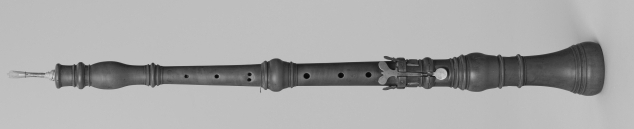
\includegraphics[width=0.9\textwidth]
{F4_09somePngOboeBaroqueDennerMIR370}%.png
}
\caption{\label{fig:asIsPng}Some PNG-picture, directly included }
\end{figure}

Note that in DVI/XDV mode all usual latex converter 
can include BMP-pictures, whereas in PDF mode only \texttt{xelatex} 
can do that, maybe because it creates XDV internally in any case. 
In contrast, \texttt{lualatex} and \texttt{pdflatex} can not. 
% The following works for lualatex but not for pdflatex 
% And still the same picture, Figure~\ref{fig:asIsPng} shows the oboe 
% as bmp-file. 

% \begin{figure}[htb]
%   \centering
%   \IfPackageLoadedTF{tex4ht}{%
%   should be a picture 
%   }{
%   \includegraphics[width=0.9\textwidth]
%   {F4_10someBmpOboeBaroqueDennerMIR370.bmp}%.bmp
%   }
%   \caption{\label{fig:asIsBmp}Some bmp-picture, directly included }
%   \end{figure}
  


\chapter{Processing of \LaTeX{} Main Files}\label{chap:latexMainConversions}

Given graphics in formats includable in TEX files, 
which may require preprocessing described in 
Chapter~\ref{chap:GraphConversions}, 
this section describes the conversions of \LaTeX{} main files 
into target files in detail. 
The most important target file format is \gls{pdf}. 
Conversion into this format is described in Section~\ref{sec:tex2pdf}. 
Note that \gls{pdf} also occurs as source format 
for included pictures and as intermediate files. 
Specific for \LaTeX{} is the \gls{dvi} format, 
which is supported mainly for historical reasons. 
% FIXME\@: nowhere described. 

Almost independent of the format created, 
inclusion of bibliographies, indices and glossaries 
requires additional conversions 
done by several auxiliary programs. 
Bibliographies are described in Section~\ref{sec:bibtex}, 
indices in Section~\ref{sec:indices} 
and glossaries in Section~\ref{sec:glossaries}. 
Only at the first sight different 
but behind the scenes quite analogous 
is inclusion of results of code evaluations, 
code in python and other languages described in Section~\ref{sec:pythontex}. 
Here, an auxiliary program essentially invokes the language interpreter. 

Sections~\ref{sec:runRerunAux} and~\ref{sec:rerunLatex} 
describe running and rerunning auxiliary programs 
like \texttt{makeindex} and the \LaTeX{} engine, respectively. 
The latter may be necessary if certain lists are present 
like table of contents list of figures or list of tables. 
Section~\ref{sec:runRerunAux} clarifies the exchange of information  
between the \LaTeX{} engines and auxiliary programs, 
whereas Section~\ref{sec:rerunLatex} 
essentially describes the exchange of information 
between individual runs of the \LaTeX{} engine. 

Section~\ref{sec:chkReprod} is special in that it is not related with conversion 
but with checking reproducibility. 
This \LaTeX{} builder has some built-in build algorithm, 
but one can also use \tool{latexmk} as a build tool 
in a way that invokes all tools with parameters given by the configuration. 
Note that \tool{latexmk} has a different build algorithm, 
but the results should be the same. 
This is mainly to integrate document development more seamlessly. 
For details on motivation and implementation see Section~\ref{sec:latexmk}. 

Besides the output formats traditional for \LaTeX, 
\gls{pdf} and \gls{dvi} describing e.g.\@ books, 
Section~\ref{sec:tex2html} describes creation of 
\gls{html}, Section~\ref{sec:tex2odt} the creation of \gls{odt} and 
Section~\ref{sec:tex2doc} creation of MS Word formats like \gls{docx}. 
Finally, also pure text can be generated 
as described in Section~\ref{sec:tex2txt}. 

\newpage


\section{Transforming \LaTeX{} files into PDF files}\label{sec:tex2pdf}

The next step is to create a PDF file from the TEX files. 
\LaTeX{} distinguishes master TEX files from TEX files intended to be inputted
from elsewhere. 
Not taking comments and that like into account, 
master TEX files roughly have the form 
%
%\lstset{language=tex, basicstyle=\small}
\begin{lstlisting}[language=tex, basicstyle=\small]
\RequirePackage[l2tabu, orthodox]{nag} % optional 
\documentclass{...}

\begin{document}
...
\end{document}
\end{lstlisting}

The core of conversion of a TEX file into a PDF file 
is running a \LaTeX{} engine \texttt{latex2pdf} 
to a master TEX file \texttt{xxx.tex}.
The \LaTeX{} engine \texttt{latex2pdf} 
is configurable via the parameter \texttt{latex2pdfCommand}. 
Possible values are \lualatex{}, \xelatex{} and \pdflatex, 
where the first is the default for which this software is also tested. 
It is also possible to pass parameters to the \LaTeX{} engine. 
Besides conversion into \gls{pdf} format, 
all engines offer conversion to the older \gls{dvi} format 
via option \texttt{-{}-output-format} as \lualatex{} and \pdflatex, 
or the alternative \gls{xdv} generalizing \gls{dvi} 
as \xelatex{} does with the option \texttt{-{}-no-pdf}. 

In fact, the engine \texttt{latex2pdf} 
does much more than converting TEX files to PDF files. 
Figure~\ref{fig:tex2pdf} shows for \texttt{latex2pdf} set e.g.~to \lualatex{}, 
that besides the PDF file also a LOG file and an AUX file is created. 
The LOG file contains logging information on the run of the conversion 
and the AUX file transports information from one run to the next, 
writing in one run and reading in the next run. 
Thus, conversion goes without it, but it is read if present. 
This is why it is depicted at input side in dashed lines. 

Optionally, an FLS file is created containing paths to the files 
the converted \LaTeX{} file depends on 
and a file with ending \texttt{synctex.gz} 
with information for mapping locations at the created PDF file 
to the according input files. 
This is to support backward search, meaning click on a place in the PDF viewer 
opens an editor in the source file. 

What is in fact in the AUX file depends on the package. 
Among other information, 
also citations and the location of the bibliography file with ending bib 
are present. 
This cannot be used directly in the next \texttt{latex2pdf} run 
to create the bibliography, 
because the entries referenced in the document must be extracted from the BIB file 
and sorted. 
This is done by invoking \texttt{bibtex} between two \texttt{latex2pdf} runs. 
Based on the AUX file, \texttt{bibtex} creates a BBL file 
containing the bibliography, which is read in the next \texttt{latex2pdf} run. 
For details see Section~\ref{sec:bibtex}. 

Alternatively to \texttt{bibtex} a bibliography can be created 
with the package \pkg{biblatex} in conjunction with the auxiliary program \texttt{biber}. 
Running a \LaTeX{} engine with package \pkg{biblatex} loaded 
creates a \gls{bcf} file read by \texttt{biber}. 
At time of this writing, this software does not support that option. 
Nevertheless, for sake of completeness we added this data path to Figure~\ref{fig:tex2pdf}. 

If an index is demanded, 
in addition \texttt{latex2pdf} creates a \gls{idx} file. 
As the citations, it cannot be used directly to create an index in
the next \texttt{latex2pdf} run, 
because the index entries must be collected and sorted before. 
This is done by invoking \texttt{makeindex} 
between the two \texttt{latex2pdf} runs. 
Based on the \gls{idx} file, \texttt{makeindex} creates a \gls{ind} file 
containing the index, which is read in the next \texttt{latex2pdf} run. 
For details see Section~\ref{sec:indices}. 

If more than one index is demanded, 
we suggest using \texttt{splitindex} instead of \texttt{makeindex} 
which creates one \gls{ind} file per index. 

A more modern technique to create an index is via \texttt{xindy}, 
but at time of this writing, this software does not support \texttt{xindy} yet. 

If a glossary is demanded, this can be read off the \gls{aux} file 
and a \gls{glo} file containing the index entries 
is created and a file with style information. 
Depending on the configuration, 
this may be a \gls{ist} file or a \gls{xdy} file. 
As for the index the \gls{idx} file, 
the \gls{glo} file cannot be used directly to create a glossary in
the next \texttt{latex2pdf} run, 
because the glossary entries must be collected and sorted before. 
This is done by invoking \texttt{makeglossaries} 
between the two \texttt{latex2pdf} runs. 
Based on the \gls{glo} file, \texttt{makeglossaries} creates a \gls{gls} file 
containing the glossary, which is read in the next \texttt{latex2pdf} run. 
For details see Section~\ref{sec:glossaries}. 

Besides \texttt{makeglossaries}, there is a more modern tool, 
\texttt{bib2gls}, which is not yet supported by this software 
at time of this writing. 

The package \pkg{pythontex} allows including python code or related 
in the \gls{tex} file and to evaluate it. 
The first \texttt{latex2pdf} run creates a \gls{pytxcode} file 
which contains essentially the code parts of the \LaTeX{} file. 
Invoking \texttt{pythontex} creates by default 
a folder \texttt{pythontex-files-xxx} 
with material where code is already evaluated. 
In the next \texttt{latex2pdf} run, this material is included in the document. 
The \pkg{pythontex} comes with a second command line utility, 
\texttt{depythontex}, eliminating all python code from the original TEX file. 
Optionally, \texttt{latex2pdf} also creates a \gls{depytx} file 
with all information to replace python code in the original TEX file 
with evaluated material from \texttt{pythontex-files-xxx}. 
Replacement is done by \texttt{depythontex} 
which by default, sends the result to stdout, 
but there is an option to write into another \LaTeX{} file. 
Converting this new \LaTeX{} file 
yields the same result as converting the original one. 
Depythonization is a feature needed e.g.~for papers 
when the publisher does not accept included code. 
For details see Section~\ref{sec:pythontex}. 

In addition, if
a table of contents, a list of figures, a list of tables 
or a list of listings is required, 
also a TOC file, a LOF file, a LOT file and a LOL file is created,
respectively, 
collecting the according information. 
Also, if hyper-references are built, an \gls{out} file 
containing bookmarks is created. 
If such a file is present, it is read in and is used
to create a table of contents, a list of figures, of tables and of listings 
or bookmarks in the second run of \texttt{latex2pdf}. 

To summarize, 
if a table of contents, a list of figures, a list of tables, a list of listings or 
a bibliography, an index or a glossary is present, 
or if code must be replaced by their evaluation, 
a second \LaTeX{} run is required to make that material appear in the PDF output. 

If a table of contents and at the same time 
a bibliography, an index or a glossary is present, 
even two further \LaTeX{} runs are required: 
After the first one, the bibliography, the index or the glossary 
occurs in the PDF file but not yet in the table of contents. 
This happens after the second additional \LaTeX{} run. 
As described in Sections~\ref{sec:runRerunAux} and~\ref{sec:rerunLatex}, 
further runs of auxiliary programs mainly to create index or glossaries, 
but also under certain circumstances bibliographies and inserting invoked code, 
followed by invocation of the \LaTeX{} engine \texttt{latex2pdf} may be necessary. 

\begin{figure}[htb]
\centering
\IfPackageLoadedTF{tex4ht}{%
should be a picture 
}{
\import{}{F5_01tex2pdf.ptx}
}
\caption{\label{fig:tex2pdf}Conversion of a TEX file into a PDF, DVI, XDV file }
\end{figure}

\section{Bibliographies}\label{sec:bibtex}

For each occurrence 
of a command \cmd{cite} in the TEX file, 
referring to a document with given key,
\texttt{latex2pdf} writes an according entry \cmd{citation} with that key 
into an AUX file. 
Note that, 
if the \LaTeX{} main file includes other TEX files with \cmd{include}, 
and the \cmd{cite}-command is invoked in the included TEX file, 
the \cmd{citation} commands go into the AUX file of that TEX file. 
Moreover, a \cmd{bibliography}-command in the TEX file 
writes a link to the BIB files containing the bibliography data 
into the (top level) AUX file as \cmd{bibdata}. 
Note that \cmd{bibliography} accepts a list of BIB files, not only a single one, 
as maybe suggested by the singular name\footnote%
{In fact, cmd{bibliography} does not only specify the (source) BIB files, 
it \cmd{input}s the (singular) bibliography to be created.}. 
The key given by \cmd{cite} commands must refer to exactly one key in the BIB files. 
Last not least, a \cmd{bibliographystyle}-command in the TEX file 
writes a link to the bibliography style file 
which determines the appearance of the bibliography 
and also the labels and the ordering 
into the AUX file as \cmd{bibstyle}. 
Typically, the style file comes from the \TeX{} distribution rather than the user. 
Its ending is \gls{bst}. 

To create a bibliography, 
a \texttt{bibtexCommand} must be run after the \LaTeX{} run. 
The default command is the traditional \tool{bibtex}, 
but there are more modern alternatives also supported
like \tool{bibtexu} and \tool{bibtex8} supporting utf8 encoding 
and others. 
Among the tools which are not supported are \tool{biber} and \tool{mlbibtex}. 

We run \texttt{bibtexCommand} if either \cmd{bibliography} or \cmd{bibliographystyle} 
is in the top level AUX file. 
If there is no \cmd{cite}-command, \tool{bibtex} yields an error. 
If neither \cmd{bibliography}-command nor \cmd{bibliographystyle}-command 
are present, then presence of \cmd{cite} yields an error when running the \LaTeX{} engine. 
So, there is an error if not either all three ingredients are present or neither. 

Essentially, \tool{bibtex} extracts the citations in the AUX files, 
unifies them, i.e.\@ a citation is listed once even if it is used more than once, 
retrieves the according entries from the BIB files specified, 
sorts and formats these entries 
according to the \gls{bst} file and writes all into a \gls{bbl} file 
which can be included in the next run of \texttt{latex2pdf}. 
Formatting includes associating a label with each key 
and sorting is based typically on the label. 
The \gls{bbl} file consists essentially in a \env{thebibliography} environment 
listing the \cmd{bibitem}s. 
These relate the key and the label given by the BST file 
and show the text of the bibliography entry. 

Note that after a \tool{bibtex}-run, 
two \LaTeX{} runs are required: 
The first one just puts the bibliography found in the \gls{bbl} file \texttt{xxx.bbl}
into the PDF file at place of \cmd{bibliography} as \cmd[\{xxx.bbl\}]{input} would do 
(which shows why \cmd{bibliography} is singular, although a list of BIB files may serve as source)
and the labels of the citations into the AUX file 
as \cmd{bibcite}-commands. 
The second run places the labels of the citations found in the AUX file 
at the citations given by \cmd{cite}. 
The package \pkg{tocbibind} described in~\cite{TocBibIndP}, 
then writes the headline of the bibliography 
into the table of contents\index{table of contents} 
if option \texttt{numbib}
% The package \pkg{rerunfilecheck} described in~\cite{RerunFChkP110}, 
% ensures that \texttt{latex2pdf} is rerun if needed, 
% provided loaded with option \texttt{aux}. 

% TBD: One could do some postprocessing to bibtex 
% writing 


This software presupposes, that \tool{bibtex} reads the AUX file 
and creates a \gls{bbl} file and also a \gls{blg} file with logging output 
as illustrated by Figure~\ref{fig:aux2bbl}. 
From the BLG file this software may determine 
whether \tool{bibtex} emitted an error or warnings. 


\begin{figure}[htb]
\centering
\IfPackageLoadedTF{tex4ht}{%
should be a picture 
}{
\import{}{F5_02aux2bbl.ptx}
}
\caption{\label{fig:aux2bbl}
Conversion of an AUX file into a \gls{bbl} file using bibliographies}
\end{figure}

Vital information on \tool{bibtex} is found in~\cite{BibPat} 
and in~\cite{BibMar}. 
Also,~\cite{Gra}, Chapter 10 is worth reading in this context. 

Note that in the master AUX file one can find also entries \cmd{bibcite} 
relating the labels for bibliography entries to the representations 
to be inserted for the \cmd{cite} commands, 
but it is the \LaTeX{} engine which extracts these mappings 
from the \cmd{bibitem} entries in the BBL file written by \tool{bibtex}. 

The package \pkg{tocbibind} described in~\cite{TocBibIndP}, 
then writes the headline of the index into the table of contents, 
if the option \texttt{numibib} is given.\index{table of contents}

% Note that also multiple bibliographies are possible: 
% for each occurrence of \cmd[\{\dots\}]{bibliography} 
% a separate bibliography is inserted furnished from the given BIB files. 
% See: latex companion \cite{LatComp2}, Section~12.6. 
% Seemingly, this is not possible with \tool{bibtex}, but I have latex companion only 2nd edition. 


\section{Indices}\label{sec:indices}

If an index is wanted, the command \cmd{makeindex} must be issued
before any index entry is requested. 
In fact, this does nothing but opening \texttt{xxx.idx} 
given a \LaTeX{} main file \texttt{xxx.tex}. 
The \gls{idx} file collects all index information extracted from \texttt{xxx.tex}. 



% \makeindex after splitindex 
% This document is an example for multiple index, 
% whereas useBeamer.tex ... (\cite needed) is an example for single index. 
% At the moment, only the perl version of splitindex is supported, not lua. 

Let us first assume that only a single index is wanted. 
For each occurrence 
of a command \cmd{index} in the TEX file, 
specifying an index entry,
\texttt{latex2pdf} writes an according entry \cmd{indexentry} 
into the \gls{idx} file 
which relates the entry with the page number where it occurred. 

For example \cmd[\{ant-task\}]{index} occurring on page 3 creates an entry 
%
\begin{lstlisting}[language=TeX]
\indexentry{ant-task}{3}
\end{lstlisting}
%
in the IDX file. 
Caution: If the IDX file is not open, 
\cmd{index} has no significant impact and in particular no index is created, 
without any warning. 

To create an index, 
a \texttt{makeIndexCommand} must be run after the \LaTeX{} run. 
The default command and the only one currently supported by this software, 
is the traditional \tool{makeindex}. 
Similar but based on unicode are \tool{upmendex} and \tool{xindex}. 
Whereas in the context of glossaries \tool{xindy} is still used, 
for pure index creation for which \tool{xindy} has been designed originally, 
it seems widely abandoned. 

Note that entries in the IDX file can occur more than once, 
even with the same page number. 
% possible to create \indexentry with section() number)s instead of page numbers? 
The task of \tool{makeindex} and related is, 
to sort the index entries given in the IDX file 
and within each entry to sort the page numbers 
unifying same page numbers and simplifying by using ranges 
and writing the result to an \gls{ind} file, 
which essentially consists of an \env{theindex} environment 
listing \cmd{item}s and \cmd{subitem}s. 


The behavior of the various \texttt{makeIndexCommand}-tools varies 
if the IDX file is empty: \tool{upmendex} does not create an \gls{ind} file at all, 
\tool{makeindex} creates and empty one and only \tool{xindex} 
creates an \gls{ind} file with an empty \env{theindex} environment. 


% In case the \LaTeX{} engine writes index information, 
% into its \gls{idx} file, at least one index must be generated. 
% Since the \gls{idx} file contains nothing but index information, 
% an index is created if and only if the \gls{idx} file is created. 
% % Well, this is not really the truth: it is needed only if ...
% Essentially, 



Then the \texttt{makeindex}-command is applied to the \gls{idx} file 
which sorts keywords and for each keyword collects the according page numbers, 
sorts it and writes the result into a \gls{ind} file. 
In the next run of \texttt{latex2pdf}, 
the \cmd{printindex}-command in the TEX file includes the index much like \cmd[xxx.ind]{input}. 
The most basic package to provide this command 
is \pkg{makeidx} described in~\cite{MkidxShIdxP}. 
In addition, \pkg{makeidx} provides the command \cmd{see} 
which is for cross-reference within an index. 
The package \pkg{tocbibind} described in~\cite{TocBibIndP}, 
then writes the headline of the index into the table of contents, 
if the option \texttt{numindex} is given.\index{table of contents}
% The package \pkg{rerunfilecheck} described in~\cite{110}, 
% ensures that \texttt{latex2pdf} is rerun if needed, 
% provided loaded with option \texttt{aux}. 

The same document,~\cite{MkidxShIdxP} 
also describes the package \pkg{showidx} 
which prints index entries at the margin of the document. 
This is for debugging only. 



This software presupposes, that \texttt{makeindex} converts the \gls{idx} file 
into an ind file containing the index 
and creating also an \gls{ilg} file with logging output 
as shown in Figure~\ref{fig:idx2ind}. 
From the \gls{ilg} file this software may determine 
whether \texttt{makeindex} emitted an error or warnings. 

\begin{figure}[htb]
\centering
\IfPackageLoadedTF{tex4ht}{%
should be a picture 
}{
\import{}{F5_03idx2ind.ptx}
}
\caption{\label{fig:idx2ind}Conversion of an \gls{idx} file into an \gls{ind} file}
\end{figure}
\medskip


The main restriction of the package \pkg{makeidx} is, 
that only a single index can be created. 
The reason is that, \texttt{latex2pdf} creates a single \gls{idx} file 
and \texttt{makeindex} creates a single ind file from that, 
representing a single index. 

To overcome this restriction, 
replace package \pkg{makeidx} and \tool{makeindex} 
with package \pkg{splitidx} and \tool{splitindex} 
both described in~\cite{SplitidxP}. 

Using package \pkg{splitidx} instead of \pkg{makeidx}, 
still the commands \cmd{index} and \cmd{printindex} can be used 
and both work as for package \pkg{makeidx}. 
Thus, also the tool \tool{makeindex} can be combined with package \pkg{splitidx}. 
This shows that \pkg{splitidx} is a full replacement of \pkg{makeidx}, 
if a single index is required besides supporting multiple indices. 

To support multiple indices, 
\pkg{splitidx} offers the command \cmd[{[\dots]}\{\dots\}]{newindex} 
to define a new index with given identifier and optional headline. 
Besides indexing command \cmd{index}, 
there is the command \cmd[{[\dots]\{\dots\}}]{sindex}, 
with optional index identifier. 

Also command \cmd{printindex} has additional variants, 
among those write all indices or write the index of a given identifier \cmd[{[\dots]}]{printindex}. 
Note that there is a special identifier, \texttt{idx} referring to the main index. 
So \cmd[{[idx]}\{\dots\}]{sindex} mainly behaves as \cmd[\{\dots\}]{sindex}. 

% TBD: clarify whether this option is for splitidx or for makeidx 
Option \texttt{split} of \pkg{splitidx} makes \texttt{latex2pdf} 
creating \gls{idx} files \texttt{xxx-y.idx} directly. 
Here \texttt{y} represents the identifier of an individual index 
which is \texttt{idx} for entries created by 
\cmd[{[idx]}\{\dots\}]{sindex}, \cmd[\{\dots\}]{sindex} and \cmd[\{\dots\}]{index}. 
These \gls{idx} files can be transformed individually with \texttt{makeindex} 
into \gls{ind} files creating log files \gls{ilg} 
as illustrated in Figure~\ref{fig:idx2indMult}. 
Since \texttt{latex2pdf} can keep open only up to 16 output streams at once, 
not all of which can be used to create a file \texttt{xxx-y.idx}, 
this approach allows a limited number of indices 
and is thus not recommended and not supported by this software. 
% Another reason is, that this approach undermines 
% the package \pkg{rerunfilecheck} described in~\cite{RerunFChkP110}, 
% and so it is not guaranteed that \texttt{latex2pdf} is rerun if needed. 
% This explains why option \texttt{split} is not allowed. 
% **** check? 

\begin{figure}[htb]
  \centering
  \IfPackageLoadedTF{tex4ht}{%
  should be a picture 
  }{
  \import{}{F5_04idx2indMult.ptx}
  }
  \caption{\label{fig:idx2indMult}
  Not supported: Conversion of \gls{idx} files into ind files}
\end{figure}
  

Instead, \pkg{splitidx} is supported without option \texttt{split}. 
Then \texttt{latex2pdf} creates a single \gls{idx} file 
but \cmd[{[y]}\{\dots\}]{sindex} 
creates lines \cmd[{[y]}\{\dots\}]{indexentry} in the IDX file 
which allow to identify the index \texttt{y}. 
For example \cmd[{[Packages]}\{pkg\}]{newindex} defines a new index of \LaTeX{} packages 
and \cmd[{[pkg]}\{splitidx\}]{sindex} on page 3 indicates 
that index there shall be an entry \texttt{splitidx} referring to page 3. 
The according entry in the IDX file is as follows: 
%
\begin{lstlisting}[language=TeX]
  \indexentry[pkg]{splitidx}{3}
\end{lstlisting}
%
Note that both \cmd[\{\dots\}]{sindex} and \cmd[\{\dots\}]{index} 
create entries \cmd[\{\dots\}]{indexentry} as with a single index. 

The program \tool{splitindex} splits up the single file \texttt{xxx.idx} 
into several \gls{idx} files \texttt{xxx-y.idx}. 
Besides the lines \cmd[{[idx]}\{\dots\}]{indexentry} 
also the lines \cmd[\{\dots\}]{indexentry} go into \texttt{xxx-idx.idx}. 
Then \tool{splitindex} applies \tool{makeindex} to each of these IDX files separately 
creating files \texttt{xxx-y.ind} and according \gls{ilg} files, 
as illustrated in Figure~\ref{fig:idx2indSplit}. 

Note that \tool{splitindex} itself does not create any kind of log file. 
Strictly speaking, there are at least two variants of \tool{splitindex} 
implemented in different languages and with slightly different behavior. 
At time of this writing, only the main variant in Perl is supported, 
but it may be interested to generalize this to the version in the Lua language. 

\begin{figure}[htb]
  \centering
  \IfPackageLoadedTF{tex4ht}{%
  should be a picture 
  }{
  \import{}{F5_05idx2indSplit.ptx}
  }
  \caption{\label{fig:idx2indSplit}Conversion of an \gls{idx} file into ind files}
  \end{figure}
  \medskip




The package \pkg{splitidx} is intended to be used 
in conjunction with the program \tool{splitindex}, 
but it can also create a single index and if so, it is better to use it in conjunction with 
\tool{makeindex} or that like. 
This software can decide on the IDX file whether there is a line specifying an index like so, 
%
\begin{lstlisting}[language=TeX]
  \indexentry[pkg]{splitidx}{3}
\end{lstlisting}
%
or neither has an explicit index, i.e.\@ like so 
%
\begin{lstlisting}[language=TeX]
  \indexentry[pkg]{splitidx}{3}
\end{lstlisting}
%
In the first case \tool{splitindex} is invoked, in the second \tool{makeindex} is invoked. 
\medskip


For usage of further packages supporting multiple indices 
which are not intended to be used with this software, 
see Chapter~\ref{chap:gaps}. 


It is possible to configure the makeindex-command 
and to pass arbitrary options. 
CAUTION\@: For the usual \texttt{makeindex}-command, 
the options \texttt{-o} specifying an output file 
and \texttt{-t} (transcript) specifying the logging file are not allowed, 
because this breaks the expectation to find the sorted index 
in file \texttt{xxx.ind} 
and bypasses the detection of errors and warnings of this software, 
respectively. 
Also specifying a style file via option \texttt{-s} 
is not recommended because this is used to create a glossary 
and so breaks glossary creation 
as described in Section~\ref{sec:glossaries}. 

Information on the makeindex program can be found in~\cite{MkIdxMoe} 
and in~\cite{MkIdxLam}. 
Also, there is a site~\cite{MakeIdxOpts} 
describing all available options for \texttt{makeindex}. 

As indicated above, the program \texttt{splitindex} 
invokes \texttt{makeindex}. 
Its options are described in~\cite{SplitidxP}, Section~3.10. 
Since the long option names are not understood in all environments, 
only the short options are recommended. 

Since \texttt{splitindex} must satisfy the interface 
given by Figure~\ref{fig:idx2indSplit}, 
the option \texttt{--help} and its shortcut \texttt{-h} are not allowed. 
Likewise for option \texttt{--version} and its shortcut \texttt{-V}. 
The option \texttt{--makeindex <makeindex>}, resp.~\texttt{-m <makeindex>}, 
is used with the \texttt{makeindex} command used for single indices. 
Thus, this may not be given explicitly but is specified implicitly. 
Also, the option \texttt{--identify <regex>}, resp.~\texttt{-i <regex>} 
must be set implicitly because it must be the same expression 
as used to ***** 
Then \texttt{splitindex.tlu} is not allowed, 
because this has another expression. 

Only allowable seems \texttt{-V}, the shortcut for \texttt{--verbose}. 

Then comes the name of the index file to be processed 
without suffix. 

The program \texttt{splitindex} invokes \texttt{makeindex}. 
The option \texttt{--} coming after the filename, 
indicates that all following options are passed to \texttt{makeindex} 



\section{Glossaries}\label{sec:glossaries}

CAUTION\@: The method described here, 
has at least two severe bugs: 
The number of reruns of the \LaTeX{} engine and also of \texttt{makeglossaries} 
is not guaranteed as a consequence of a bug in \pkg{rerunfilecheck} 
and the fact, that it does not fit current versions of \pkg{makeglossaries}. 
In addition, entries of the glossaries not mentioned directly in the document 
but must be included because they are used in the explanation of entries to be included 
are not treated properly. 

As a consequence, this document, or to be more precise its glossary, 
could not always be reproduced and so the author excluded the glossary until the problem is fixed. 

In addition, it is a conceptual weakness that a glossary data base 
shall be centralized and shall thus not be included in a \LaTeX{} document 
and not even be written in \LaTeX. 
All weaknesses, bugs and conceptual shortcomings are overcome 
by the package \pkg{glossaries-extra} in conjunction with the auxiliary program \texttt{bib2gls} 
which will replace \pkg{glossaries} and \texttt{makeglossaries}. 
For the time being, use glossaries with caution. 
\medskip


Creating glossaries 
requires the package \pkg{glossaries} described in~\cite{GloP4_54}. 
By default, package \pkg{glossaries} creates a single ``main glossary'', 
which can be switched off specifying the option \texttt{nomain} 
described in Section~2.6. 
In this case at least, more specific glossary types with according headline must be specified. 
As specified in~\cite{GloP4_54}, Section~2.6, 
\pkg{glossaries} offers \texttt{acronyms}, \texttt{symbols},
\texttt{numbers} and \texttt{index}. 
To avoid collision with indexing as described in Section~\ref{sec:indices}, 
this software does not allow the latter. 
Moreover, the package \pkg{glossaries} even supports user-defined glossary types, 
but this software does not, 
mainly to keep the internal build in line with build using \tool{latexmk}. 
For details see Section~\ref{sec:gapGlossaries}. 

Also, the package \pkg{glossaries} offers sorting and unifying 
either via \texttt{makeindex} as for indices or via \texttt{xindy}, 
and it offers also to do without external programs. 
In contrast, this software supports only the variant using \texttt{makeindex}. 





As for creating indices there is a \LaTeX-command \cmd{makeindex}, 
to create a glossary there is a \LaTeX-command \cmd{makeglossaries}, 
but the latter is not built-in as \cmd{makeindex} 
but provided by the package \pkg{glossaries}. 
If \texttt{xxx.tex} is the \LaTeX{} main file, 
\cmd{makeglossaries} opens the glo file \texttt{xxx.glo} 
containing glossary entries for writing. 
As the built-in command \cmd{index} 
writes entries into the \gls{idx} file defining the index, 
the command \cmd{gls} defined by the package \pkg{glossaries} 
writes an entry into the glo file. 
Note that \texttt{xxx.glo} typically contains entries more than once 
and that the entries are not sorted. 

To perform sorting, formatting and typically also unification, 
the package \pkg{glossaries} allows three mechanisms. 
This software supports two of them: 
via the shell command \texttt{makeindex}, which is also used for indices, 
and via the shell command \texttt{xindy}. 
Using \texttt{makeindex} is the default but can also be activated through 
\cmd[{[makeindex]}\{glossaries\}]{usepackage}. 
Using \texttt{xindy} instead of \texttt{makeindex} is triggered through 
\cmd[{[xindy]}\{glossaries\}]{usepackage}. 
Accordingly, for option \texttt{makeindex} the AUX file receives lines 
%
\begin{lstlisting}[language=TeX]
\providecommand\@istfilename[1]{}
\@istfilename{manualLMP.ist}
\end{lstlisting}
%
whereas for option \texttt{xindy}, there are lines 
%
\begin{lstlisting}[language=TeX]
\providecommand\@istfilename[1]{}
\@istfilename{manualLMP.xdy}
...
\providecommand\@xdylanguage[2]{}
\@xdylanguage{main}{english}
\providecommand\@gls@codepage[2]{}
\@gls@codepage{main}{}
\end{lstlisting}



This software neither invokes \texttt{makeindex} nor \texttt{xindy} directly. 
Instead, it invokes the shell command \texttt{makeglossaries}
invoked without file ending  
which determines from the AUX file 
whether to invoke \texttt{makeindex} nor \texttt{xindy}. 
Accordingly, it writes the style definition 
by creating an ist file \texttt{xxx.ist} or an xdy file \texttt{xxx.xdy} 
if \texttt{makeindex} or \texttt{xindy} is specified as package option, 
respectively. 

Seemingly, \texttt{makeglossaries} relies on the AUX file 
to determine whether to invoke \texttt{makeindex} or \texttt{xindy} 
for sorting and unification. 
Then it invokes the according command and writes a LOG file 
with ending \texttt{glg}, 
redirecting the logging output of \texttt{makeindex} or \texttt{xindy} 
adding own output so that a glg file may be written, 
even if e.g.~\texttt{makeindex} is invoked and does not. 
In any case, if the glg file is written, 
\texttt{makeglossaries} writes text matching 
%
\begin{verbatim}
(^\*\*\* unable to execute: )
\end{verbatim}
%
in the glg file if an error occurs, 
no matter whether \texttt{makeindex} or \texttt{xindy} is invoked. 
Possibly, there are cases where an error causes no glg file to be written. 
If no error occurs, a glg file is written 
and if warnings are emitted, 
they either come from \texttt{makeindex} or from \texttt{xindy}. 
Thus warnings may be detected with the patterns 
defined by \texttt{makeindex} and by \texttt{xindy}. 

The style \texttt{list} (which is the default) is set in the form 
%
\begin{lstlisting}[language=TeX]
\usepackage[style=list]{glossaries}
\end{lstlisting}
%
where~\cite{GloP4_54}, Section~13 lists predefined styles. 
So, the style determines the content of the style definition, 
whereas the options \texttt{makeindex} and \texttt{xindy} 
specify the form in which the style is encoded 
and thus the ending of the style file, 
which is either \texttt{ist} or \texttt{xdy}. 

Sorting the glo file, as said above, 
currently is only supported using the command \texttt{makeglossaries}. 
The allowed options are essentially those 
making sense for \texttt{makeindex} and those making sense for \texttt{xindy}. 
If the shell command \texttt{makeglossaries} 
invokes \texttt{makeindex} of course only the according options 
are passed supplemented by additional options 
\texttt{-s}, \texttt{-t}, \texttt{-o}, to specify the
ist file, the glg file (the transcript file) and the gls file,
respectively, 
which is the result of sorting, the output file, 
and contains the entries of the glo file 
just sorted, formatted and unified.
So for a tex main file \texttt{xxx.tex} the program 
\texttt{makeglossaries} invokes
%
\begin{verbatim}
makeindex  -s "xxx.ist" -t "xxx.glg" -o "xxx.gls" "xxx.glo"
\end{verbatim}
%
Accordingly, if the shell command \texttt{makeglossaries} 
invokes \texttt{xindy} of course only the according options 
are passed supplemented by additional options 
\texttt{-M}, \texttt{-t}, \texttt{-o}. 
This is illustrated in Figure~\ref{fig:glo2gls}. 


\begin{figure}[htb]
\centering
\IfPackageLoadedTF{tex4ht}{%
should be a picture 
}{
\import{}{F5_06glo2gls.ptx}
}
\caption{\label{fig:glo2gls}Conversion of a glo file into a gls file 
using \texttt{makeglossaries}}
\end{figure}


\section{Including code via \texttt{pythontex}}\label{sec:pythontex}

The package \pkg{pythontex}, described in~\cite{PythonTexP} 
originally allowed including Python code into a latex document. 
Later on, further languages were added, most notably octave or Matlab, 
and the user can easily extend it to further languages 
as sketched in~\cite{PythonTexP}. Section 7. 
Of course, to that end, the interpreter for the desired language must be installed.\index{pythontex}
The meaning of the term ``including'' used above 
ranges from mere listing to pure execution and comprises also inserting results of execution. 
A field of application is also creating figures. 

Note that like the package \pkg{splitindex}, also \pkg{pythonindex} 
comes with an according auxiliary program, 
in this case, besides \texttt{pythontex} also \texttt{depythontex}. 
Consequently,~\cite{PythonTexP} is not only on the package 
but also on the corresponding command line tools. 
Since~\cite{PythonTexP} is quite detailed, 
there is an introduction~\cite{PythonTexQ} and a gallery~\cite{PythonTexG}. 
For background on the intentions of package \pkg{pythontex}, consult~\cite{PythonTexRepr}. 
Information required to integrate pythontex into this software 
partially goes much beyond the official documentation and is collected in~\cite{PyTexInOut}. 
It could also be interesting for the user for debugging. 

Running the \LaTeX{} engine on a file \texttt{xxx.tex} 
with package \pkg{pythontex} loaded 
yields a file \texttt{xxx.pytxcode} 
and if the package is loaded with option \texttt{depythontex} 
also a file \texttt{xxx.depytx}.
If the file \texttt{xxx.pytxcode} is present, 
this software invokes the command line tool \texttt{pythontex} 
(same name as the according package) 
to \texttt{xxx.pytxcode} (without ending) 
which converts this into a variety of output files, 
which are, without further configuration, 
all in the folder \texttt{pythontex-files-xxx}
as shown in Figure~\ref{fig:py2dir}, 
which is described in more detail in~\cite{PyTexInOut}, Section~3. 
Note that this software uses the wrapper \texttt{pythontexW}\index{pythontexW} 
of \texttt{pythontex} described in Section~\ref{subsec:pythontexW}, 
instead of \texttt{pythontex} itself. 
The figure reflects this. 

% TBD: later on, if \texttt{xxx.depytx} after \texttt{pythontex} also \texttt{pythontex} is invoked, 
% creating a TEX file without python code. 
% TBD: clarify what if input files or include files are present. 

Running the \LaTeX{} engine again, 
includes all the output files \texttt{*.stdout} 
in the PDF file or whatever output file created. 

% Note that if depythontex is invoked, it is immaterial whether the subsequent run of LaTeX-to-pdf converter 
% is on the original TEX file or on the TEX file created by depythontex. 

An important remark is that \lualatex{} is the preferred engine, 
because files \texttt{*.stdout} can impose heavy memory usage 
and currently \lualatex{} is the only engine allocating memory dynamically. 

As one can see, \texttt{pythontex} cooperates with \lualatex{} in a way 
also \texttt{bibtex} or the other auxiliary programs do. 
Although \texttt{pythontex}, at time of this writing in version 0.18, 
is quite mature, it refrains from writing a log file and indicates errors and warnings 
just on standard output or error output. 
This is unlike all the other auxiliary programs in a line with \texttt{pythontex}. 
As a consequence, in particular warnings are difficult to detect 
and cannot be detected in a uniform way. 
Thus, the author wrote a little wrapper, called \texttt{pythontexW} 
and place it where it can be found, e.g.~in the folder of \texttt{pythontex}. 

Accordingly, \texttt{depythontex} behaves in a non-standard way: 
Firstly, by default, it does not output a result file but outputs on standard output. 
This can be changed using the option \texttt{--output} or \texttt{-o} for short. 
Also, \texttt{depythontex} changes into interactive mode 
if the output file is already present. 
To avoid this, the option \texttt{--overwrite} is required. 
Overwriting without asking is the standard behavior of all other auxiliary programs. 
As \texttt{pythontex} also \texttt{depythontex} does not write a log file 
but just prints its errors and warnings. 
Thus, the author wrote a little wrapper, 
called \texttt{depythontexW} and described in Section~\ref{subsec:pythontexW}, 
and place it where it can be found, e.g.~in the folder of \texttt{depythontex}\index{depythontexW}. 
% TBD: evaluate: maybe it is a better solution to enable this software itself to write the output to a log file. 
\medskip


The package \pkg{pythontex} and the according auxiliary programs are highly configurable, 
more than this software allows. 

In particular, in the \LaTeX{} document, 
the commands \cmd{setpythontexoutputdir} setting the output directory 
and \cmd{setpythontexworkingdir} setting the working directory shall not be used, 
because this software assumes the default, that the working directory is the directory 
containing the \LaTeX{} main file \texttt{xxx.tex}
and the output directory is in the working directory 
and its name is \texttt{pythontex-files-xxx}. 

Further, the package \pkg{pythontex} can be configured with package options when loading the package. 
Since this software is designed for reproducibility, 
most appropriate would be to specify \texttt{runall=true} meaning that even if no python code is modified 
the auxiliary program \texttt{pythontex} executes the python code in the document. 
Also, it is appropriate to specify \texttt{rerun=always}. 
Note that the defaults are \texttt{runall=false} and \texttt{rerun=errors}. 
This behavior makes sense to speed up creation of the document, 
but it differs from the behavior of all other auxiliary programs 
and causes the check for update of output files to fail. 
Moreover, reproducibility is not as easily shown. 

The package documentation~\cite{PythonTexP} suggests, 
that this makes a difference between \texttt{runall=true/false} 
and \texttt{rerun=always/errors} if external sources are modified, 
but as is proved in~\cite{PyTexInOut}, Section 2.1, 
the package translates package option \texttt{runall=true/false} into key value pair \texttt{rerun=always/errors} 
and this is the only information \texttt{pythontex} obtains from the package, 
so there is no difference. 

Also, the auxiliary program \texttt{pythontex} itself can be configured via command line arguments. 
For the package options \texttt{runall} and \texttt{rerun}, 
there are according command line options \texttt{-{}-runall} and \texttt{-{}-rerun} with the same scope. 
Whereas the package merges options \texttt{runall} and \texttt{rerun} silently, 
the auxiliary program \texttt{pythontex} emits an error, if both are combined. 
Essentially one can forget about \texttt{runall} and stick to \texttt{rerun}. 

Strange enough, according to~\cite{PythonTexP}, Section 4.1, package options overwrite command line options. 
This software shall invoke \texttt{pythontex} 
with the option \texttt{-{}-rerun=always} which is thus specified as the default. 
To force unconditional update, this is not sufficient. 
Instead, this software relies on an undocumented feature of auxiliary program \texttt{pythontex} 
which is likely not to change: 
If one of the expected output files is missing, it recreates all output files, independent of command line options and package options. 
Thus, this software deletes one output file if present, before executing \texttt{pythontex}. 

When this software invokes \texttt{pythontex} 
the exit codes may not be changed via \texttt{-{}-error-exit-code}, 
i.e.~if specified then with value \texttt{true}. 
Neither the options \texttt{-{}-interactive}, \texttt{-h}, \texttt{-{}-help} or \texttt{-{}-version} are allowed. 
Currently, this software does not check for options which are not allowed. 
Fortunately, the latter two command line options have no counterpart in the package configuration. 




If we place some code, e.g.~python code as inline code using \cmd{pyc}
%
\begin{lstlisting}[basicstyle=\footnotesize]
  \usepackage[depythontex]{pythontex}
  ...
  \pyc|print(rf'Python inside latex says: "Hello World; 1+1={1+1}"')|
\end{lstlisting}
%
the code is really evaluated, and the string result is included at proper place 
as illustrated by the following text which is created by python: 
%
\begin{quote}
  \texttt{\pyc|print(rf'Python inside latex says: "Hello World; 1+1={1+1}"')|}. % chktex 26  chktex 18 chktex 36
\end{quote}
%
Note that the typewriter font is not created by python, 
it is explicitly set to highlight the string created by python, 
but it is python which evaluates the little computation 
and which prints the string. 

Since \texttt{pythontex} is written in python, 
including python code in the \LaTeX{} document 
uses the python interpreter already installed, as a prerequisite of \texttt{pythontex}. 
To use another language, the according interpreter must be installed in addition to python. 



% TBD: create a figure 


% TBD: depythontex


\begin{figure}[!htb]
  \centering
  \IfPackageLoadedTF{tex4ht}{%
  should be a picture 
  }{
  \import{}{F5_07py2dir.ptx}
  }
  \caption{\label{fig:py2dir}Conversion of a \texttt{pytxcode} file using \texttt{pythontex}}
  \end{figure}


  Figure~\ref{fig:depy2out} shows the files converted by \texttt{depythontex}. 
  As for \texttt{depythontex}, this software uses the wrapper \texttt{depythontexW} 
  of \texttt{depythontex} instead of \texttt{depythontex} itself. 
  This is reflected in the figure. 


  \begin{figure}[!htb]
    \centering
    \IfPackageLoadedTF{tex4ht}{%
    should be a picture 
    }{
    \import{}{F5_08depy2out.ptx}
    }
    \caption{\label{fig:depy2out}Conversion of a \texttt{depytx} file using \texttt{depythontex}}
    \end{figure}
  
\section{Running and rerunning auxiliary programs}%
\label{sec:runRerunAux}

After describing the interface 
between the \LaTeX{} engine and the auxiliary programs 
in Section~\ref{subsec:latexAux}, 
Section~\ref{subsec:noRerunfilecheck} explains 
why we don't use the package \pkg{rerunfilecheck} 
to determine when to (re-) run auxiliary programs. 


\subsection{The interface between \LaTeX{} and auxiliary programs}%
\label{subsec:latexAux}

Auxiliary programs perform tasks which \LaTeX{} cannot carry out at all 
or only with bad performance, 
for example adding bibliographies which comprises sorting 
or executing program code. 

The interface between the \LaTeX{} engine and an auxiliary program 
is always implemented via files: 
In the first run, the \LaTeX{} engine writes a file or files 
specific for the auxiliary program 
or at least writes entries specific for the auxiliary program 
in a standard file or even both. 
Then the auxiliary program is run which creates other files 
which in turn must be read back, in a second run of the \LaTeX{} engine. 
So the run of an auxiliary program 
is always enclosed between two runs of a \LaTeX{} engine. 

Typically, the \LaTeX{} run needs a \LaTeX{} package 
associated with the auxiliary tool 
which performs reading and writing. 
An exception is \tool{bibtex} and friends 
for which \LaTeX{} engines support communication out of the box. 
An example with more complicated communication 
is \tool{makeglossaries} with associated package \pkg{makeglossaries} 
which writes lines into the AUX file 
and which typically writes the main glossary into a GLO file. 
The tool \tool{makeglossaries} which is invoked without ending, 
reads the AUX file, determines which other files to read, 
typically the GLO file also 
and writes the result into the GLS file. 
This is read back by the package \pkg{makeglossaries} 
in the next run of the \LaTeX{} engine. 


\subsection{When running an auxiliary program}\label{subsec:firstRunAux}

After the first run of the \LaTeX{} engine, 
one must decide which auxiliary programs to run. 
For each auxiliary program, there is a specific file it reads 
or at least specific entries in a general file, typically the AUX file. 
If this file or these entries exist, the auxiliary program must be run 
and after the \LaTeX{} engine must be rerun 
to read in the data created by the auxiliary program. 
As is discussed for each auxiliary program separately 
in Section~\ref{subsec:noRerunfilecheck}, 
this file or these entries may change after each run of the \LaTeX{} engine 
and as a result, the auxiliary program must be rerun as well. 
So, \LaTeX{} engine and auxiliary program maybe must be run alternately. 

Instead of checking whether the relevant data really changes, 
only the number of relevant lines and a hash is taken into account. 
% TBD: clarify: Does it really have advantages to take the number of lines into account? 
% latexmk uses the length instead. 
% is it advantageous to add length as additional identifier 
% or instead number of lines? 
% Maybe some discussion is in place 
This bears a minimal risk of not rerunning the auxiliary program although needed. 
Note that also package \pkg{rerunfilecheck} is based on hashes and bears the same risk. 
% TBD: could improve just compressing the entries losslessly. 
% Essentially, there is a whole spectrum between hashes with high overlap 
% and hashes with no overlap, i.e.\@ lossless. 
% Maybe even Hamming distance plays a role. 

It is an interesting detail, 
that deciding whether an auxiliary program must be run at all, 
i.e.\@ for the first time, 
is just based on the existence of a specific file 
or of a specific line in a file, 
not comprising all pieces of information read by the auxiliary program. 
Nevertheless, if it is decided that the auxiliary program must be run, 
it is clear that the \LaTeX{} engine must be run after also 
and so the information may change. 
So one must be prepared for a rerun check. 
For this, all the information in the file(s) %chktex 36
relevant for the auxiliary program must be hashed. 

From the second run of the \LaTeX{} engine on, 
only those auxiliary programs must be checked for rerun condition, 
for which a hash is present. 
\medskip

After these quite abstract considerations, 
let us apply these to the concrete auxiliary programs supported. 





% TBD: \pkg in headlines 
\subsection{Why \texttt{rerunfilecheck} is not used for auxiliary programs}%
\label{subsec:noRerunfilecheck}

As described in Section~\ref{sec:prerequisites}, 
package \pkg{rerunfilecheck} is used to check 
whether the \LaTeX{} engine must be rerun, 
and its authors also intended it to check 
for need of rerun of auxiliary programs. 
While this works satisfactory for a single index, 
it fails for multiple indices. 
Likewise, support for glossaries is buggy and works only in case of a single glossary, 
which in addition must be the main glossary. 
In contrast, the package \pkg{glossaries} supports multiple glossaries, 
with and without main glossary 
and even allows user-defined glossaries. 
It is awkward to implement rerun check 
for all this functionality with \pkg{rerunfilecheck}. 
% TBD: link to discussion for rerun check on bibliography and others.. 

It may be surprising, that there are situations 
where even bibliography processors need to be rerun, 
among these backlinks, and citations in headlines and glossaries. 
Package \pkg{rerunfilecheck} does not take this into account. 
Accordingly, even \texttt{pythontex} may need a rerun, 
e.g.\@ if code is executed in headlines or in captions of floating objects, 
because this may insert additional invocations and may change invocation order 
which may lead to different results. 

While many auxiliary programs depend only on a subset of entries 
in their source file, 
\pkg{rerunfilecheck} can take files into account only as a whole. 
As a consequence, even if no rerun is required 
because the relevant entries did not change, 
\pkg{rerunfilecheck} could trigger useless rerun, 
because irrelevant entries in the relevant file changed. 

Tanking all these aspects into account, 
we decided to provide an internal algorithm for rerun check of auxiliary programs, 
which is based on the ideas of \pkg{rerunfilecheck} 
but avoiding all its shortcomings. 

Note also, that besides whether to rerun an auxiliary program, 
there is also the question in which case to run it at all, i.e.\@ for a first time. 
Since package \pkg{rerunfilecheck} interprets a newly occurring file 
as a changed file, this case is addressed implicitly. 

Unfortunately, not all packages associated with auxiliary tools 
give a hint if the auxiliary program must be run. 
% TBD: talk with the maintainers 
\medskip


As described in Section~\ref{sec:tex2pdf}, 
running a \LaTeX{} engine as \texttt{latex2pdf} 
may detect the presence of a bibliography, an index and/or of a glossary 
and writes raw files to describe them. 
After that, an intermediate step is required, 
sorting, unifying and formatting the entries. 
This is always done by an external program, we call an auxiliary program. 
Similarly, the presence of code to be interpreted 
may be detected which is also written in a separate file 
and an external program, 
\tool{pythontex} must be run to run the code in sequence 
and in many cases to determine the result of invocation. 

In the next step, 
the \LaTeX{} processor must read in the results of the auxiliary programs again 
to write bibliography, indices and glossaries 
and to insert the results of code invocations. 
Also, except the code invocations, 
all other pieces of information typically go into the table of contents. 
If code is invoked in a headline or in a caption, 
the result of the code invocation goes into the TOC and in the list of captions, 
e.g.\@ the list of figures LOF also. 
So in any case, after an auxiliary program the \LaTeX{} processor must be rerun. 

Obviously, the run of a \LaTeX{} processor may change page numbers 
and thus invalidate the index or the glossary. 
So the auxiliary program to create the index or the glossary must be rerun 
if the \LaTeX{} processor changes the input file for the auxiliary program 
creating index or glossary and after that, 
the \LaTeX{} processor must be run again. 

What is less obvious is, that bibliographies may be invalidated also, 
e.g.\@ because of a backlink 
or because a bibliographic reference occurs in a glossary. 
Even code may be invalidated by a run of the \LaTeX{} processor 
if some code occurs in a floating object, e.g.\@ in the caption or in a glossary. 
So code invocations may change order 
and also there may be additional code 
occurring not before later runs of the \LaTeX{} processor. 
So also in this case, the according auxiliary program, \tool{pythontex} 
must be rerun after the run of the \LaTeX{} processor. 

Summarizing, a run of the \LaTeX{} processor 
may trigger invocation of each auxiliary program. 
This must be done if the according raw file changes. 
Note that various auxiliary programs share the AUX file to get information. 
So only the aspects relevant for the specific auxiliary program 
shall be taken into account. 
What makes things a bit more complicated is, 
that including TEX files yields included AUX files 
which must be taken into account also. 

To implement rerun check completely reliable, 
huge parts of text files, a lot of information must be stored. 
Thus, we go a way like package \pkg{rerunfilecheck}, 
detecting only the change of number of relevant lines and the according hash. 
In extremely rare cases, this software may fail to rerun a program although needed, 
because number of relevant lines or its hash don't change 
although contents change. 

Note that we only use the concept of \pkg{rerunfilecheck} 
to detect running and rerunning auxiliary programs, 
but we do not use the package \pkg{rerunfilecheck} itself for this task. 
This is because supporting all relevant auxiliary programs and also 
included AUX files would require considerable extensions on \pkg{rerunfilecheck} 
and would impact considerable dependencies. 
So, as described in Section~\ref{sec:rerunLatex}, 
\pkg{rerunfilecheck} is used to control rerunning the \LaTeX{} processor 
as far as auxiliary programs are not involved, 
whereas detecting auxiliary programs to be rerun is done internally 
while the algorithm is inspired by the package \pkg{rerunfilecheck}. 


\section{Rerunning the \LaTeX{} processor}\label{sec:rerunLatex}

CAUTION\: rework needed 

FIXME\@: a word on change in toc, lof, lot and lol. 

As indicated in the previous sections, 
\texttt{latex2pdf} must be rerun, 
if an auxiliary program like \texttt{bibtex}, \texttt{makeindex} 
or \texttt{makeglossaries} 
had been run. 

Likewise, if a toc file, a lof file, a lot file or a lol file
had been created in the first \texttt{latex2pdf} run, 
another run is needed to read in these files 
to create a table of contents, a list of figures or a list of tables, 
respectively. 
Note that for all these cases, 
the LOG file does not allow to detect that \texttt{latex2pdf} has to be rerun, 
by matching a fixed pattern. 

After the second run of \texttt{latex2pdf}, 
the table of contents,
the list of figures, the list of tables and the list of listings 
are included and a section with the bibliography, 
the index and the glossary are inserted. 
It takes a third run of \texttt{latex2pdf} 
to include the bibliography the index and the glossary 
into the table of contents. 
Also, it takes that third run to replace the citations 
with the proper labels given in the bibliography. 

Inserting the table of contents,
the list of figures, the list of tables and the list of listings 
may shift the subsequent text 
which may require another run of \texttt{latex2pdf} 
to get the page numbers right. 
As described in Section~\ref{sec:runRerunAux} 
intermediate runs of auxiliary programs like \texttt{makeindex} 
may be required 
and these also require another run of \texttt{latex2pdf} 
also to get the page numbers right. 

The package \pkg{rerunfilecheck} allows detecting file changes via a hash 
almost for sure, and writes an according message into the LOG file. 
This is offered for pure rerun control of \texttt{latex2pdf} 
based on TOC, LOL, LOF and LOT, but also on the OUT file written by package \pkg{hyperref}. 
Partially, it supports also the need to rerun auxiliary programs, 
but for sake of uniformity, we refrain from using this, 
and rely on in internal algorithm also based on hashes. 

Only for rerunning \texttt{latex2pdf} alone, we rely on package \pkg{rerunfilecheck}. 
This software just reruns texttt{latex2pdf} 
if it detects the pattern of warning written by \pkg{rerunfilecheck} into the LOG file. 



Note that there are several packages which require additional runs, 
such as the package \pkg{longtable}, 
which may vary dimensions of tables. 
This software presupposes, that all these reruns 
may be detected by matching a fixed pattern in the LOG file. 
Since packages are frequently changed and new packages are written, 
also the pattern cannot be fixed. 
Thus, it is configurable. 
 
Note that, if a package requires running other programs 
between two runs of \texttt{latex2pdf}, 
this may require a change in this software. 

\section{Checking reproducibility}\label{sec:chkReprod}

There are use cases, where it is extremely important 
that the according artifacts are really reproducible. 
One is when we have to deliver the sources 
and the receiver has to reconstruct the artifacts. 
Another obvious use case is integration test for this software 
by ensuring that each artifact created 
is equivalent with a confirmed version, 
although this software changed. 
Details are given in Section~\ref{chap:tests}. 


Currently, reproducibility checks are supported for PDF files only. 
% TBD: change that 
The problem with PDF files is, that besides visible contents 
they contain also metadata (see~\cite{Pdf17} or~\cite{Pdf20}, each Section 14.3), 
which depends on the run of the conversion. 
For example the timestamp and the timezone of conversion goes into 
and derived from these other values. 

There are two strategies to deal with the problem: 
%
\begin{itemize}
  \item 
  Make the build process reproducible. 
  The advantage of this approach is that diffing is quite simple, 
  fast and reproducible: it is byte by byte. 
  This is easily done with a fixed installation 
  but tends to break with update of tools. 
  % TBD: allow own version check. 
  % Also, at time of this writing, 
  % the different latex engines cannot be treated uniformly. 
  % TBD: a feature request to hyperref is already posted. 
  % let us keep an eye on that. 
  \item 
  Use diff tools implementing a weaker notion of equivalence, 
  in a sense visibility equivalence of some degree. 
  One approach is the script \texttt{vmdiff} 
  described in Section~\ref{subsec:pythontexW} 
  which combines visibility equivalence 
  with equivalence of part of metadata. 
\end{itemize}%

Since the first one works very well, it is the one we describe here, 
but it is always possible to configure a diff tool with a weaker equivalence check. 

The first question is, whether reproducibility is requested. 
It is, if there is according magic comment in the \LaTeX{} main file requires this 
as described in Section~\ref{subsubsec:openingMagComm}. 
If there is no such magic comment is present, if the setting \texttt{chkDiff} specifies so. 
If in this section settings are given without explicit reference, 
they are described in Table~\ref{tab:paramDiffPdf} on page~\pageref{tab:paramDiffPdf} 
in Section~\ref{sec:paramRepro}. 

Since date and time both visible and in the metadata of a PDF document 
is given relative to a timezone, 
for reproducible builds compilers must run with a fixed timezone 
and, as reproducibility shall not break if changing a timezone 
or if the country running the build changes between daylight saving time and standard time, 
we chose a uniform timezone namely UTC\@. 

If a \LaTeX{} main file is already under reproducibility control, 
then there is an according original PDF file in \texttt{diffDirectory} or in a subfolder 
to be compared with a newly created PDF file 
which occurs in a subfolder of the TEX source directory \texttt{texSrcDirectory} 
described in Table~\ref{tab:paramGen} on page~\pageref{tab:paramGen}. 
The PDF file for comparison has the same path relative to \texttt{diffDirectory} 
as the created PDF file relative to \texttt{texSrcDirectory}. 

First \texttt{pdfMetainfoCommand} is used 
to extract metadata \texttt{CreationTime} from the original PDF file. 
This comprises time and timezone which is UTC\@. 

The compilation to create the new PDF file is run in an environment 
with that timezone and with that creation time. 
In addition, there is an environment variable forcing 
that the timestamp does not only affect metadata but also visual data of the PDF file 
to be created, 
as e.g.\@ typically the date at the front page. 
Note that if the PDF file is created from TEX files via DVI/XDV files, 
both engines need the appropriate environment. 

After creating the new PDF file with this environment, 
coincidence with the original PDF file is checked 
using the tool given by setting \texttt{diffPdfCommand} described in Table~\ref{tab:paramDiffPdf}. 
If the actual artifact does not coincide with predefined one 
according to the chosen diff tool, 
a build exception is thrown as specified in Table~\ref{tab:TLP}. 
\medskip


If a \LaTeX{} main file is not already under reproducibility control, 
then no original PDF file exists. 
In this case, the environment for compilation only ensures the timezone UTC\@. 
Then the created PDF file is copies at proper place into \texttt{diffDirectory} 
-- that's all for setting a document under reproducibility control. 

Finally, if a \LaTeX{} main f8ile file is under reproducibility control 
but is to be changed in a way that also the according PDF file is affected, 
then before compilation just the original PDF file is deleted, 
and the workflow is as setting under reproducibility control. 
\medskip


Reproducibility is affected or even supported by various injections 
as defined in Section~\ref{sec:injFiles}. 
First, the generic header described in Section~\ref{subsec:header} 
affects metadata, above all because it loads the package \pkg{hyperref}. 
Part of this metadata is overwritten by another header 
described in Section~\ref{subsec:headerSuppressMetaPDF}, 
to improve security and privacy, 
but enough metadata remains to keep up reproducibility. 
Reproducibility is guaranteed with the full set of metadata 
or with somehow reduced metadata. 
The only piece of information needed for reproducibility is \texttt{CreationDate} 
and this is preserved by the headers. 
Removing this also has severe consequences 
so that we can assume it is preserved. 
On the other hand, removing metadata may stabilize reproducibility 
as this is true for the banner which identifies the latex compiler and its version 
and consequently breaks reproducibility in any version change. 
Details to reproducibility with a focus on metadata are given in~\cite{LatexGen}, Section 4. 

Obviously, reproducibility checks cause work 
when putting a document under check, 
i.e.\@ in the end phase of document development 
as defined in Section~\ref{sec:devel}
or if the source document changes, i.e.\@ if document development is entered again, 
or if the output PDF changes unintended 
normally, although the sources did not change in an obvious way, 
which triggers again document development searching the cause of the change in the sources. 

This \LaTeX{} builder is not the tool for document development. 
Instead, Section~\ref{subsec:develLatexmk} suggests to use \tool{latexmk} for, 
and describes how \tool{latexmk} is integrated in this \LaTeX{} builder: 
This builder writes a config file \texttt{.latexmkrc} 
reflecting the settings of this software, at least to some extent. 
The config file \texttt{.latexmkrc} is again written as an injection 
and is described in Section~\ref{subsec:latChkRc}. 
It supports reproducibility checks even reading magic comments, 
checking existence of original PDF file 
and reading its timestamp if the PDF file is present. 
Creation of the new PDF file takes timestamp and timezone into account. 

Two further injections may be helpful in the context of reproducibility checks, 
both described in Section~\ref{subsec:ntlatexVmdiff}: 
\tool{ntlatex} to create a PDF file and \tool{vmdiff} 
realizing a weaker variant of diffing tool as described above: 
It checks for visual equality and equality of metadata. 
% TBD: maybe not true: only in trailer directory of the PDF. 
\medskip


For updating metadata only, we suggest the following technique: 
Keep the original PDF file in \texttt{diffDirectory} 
and check with \tool{vmdiff} that visually, the PDf file remains the same 
and that the correct metadata is updated. 
Of course, a new timestamp is wanted. 
So in a second step, the original PDF file is deleted, 
compilation is repeated, e.g.\@ by \tool{ntlatex} and copied into \texttt{diffDirectory}. 
\medskip


There are rare occasions where the timestamp shall be set explicitly. 
This is not possible directly as it is read off from the original PDF file. 
We suggest to use \texttt{exiftool} to modify the \texttt{CreationDate} 
of the original PDF file in \texttt{diffDirectory} before compilation. 
This is done by something like
%
\begin{verbatim}
  exiftool -PDF:CreateDate=2020-01-01T00:01:02Z xxx.pdf 
\end{verbatim}
%
Here, the option \texttt{PDF:CreateDate} is in fact the name of the tag to be written. 
Note that the timezone must be UTC represented by the \texttt Z 
signifying zero time offset compared to UTC\@. 
The attentive reader may wonder why the option is \texttt{PDF:CreateDate} instead of \texttt{CreationDate}. 
One may check with \texttt{pdfinfo}, that really \texttt{CreationDate} is modified. 
Note that \tool{exiftool} writes the original PDF file into \texttt{xxx.pdf\_original}

Two important details are not so obvious: 
%
\begin{itemize}
\item
Not only the given metadata is changed but also all metadata depending on it, 
in this case the trailer ID\@. 
This is to keep the PDF file consistent. 
\item 
The metadata is not really overwritten, but it is hidden by new metadata. 
In fact, \texttt{exiftool} uses incremental update specified for the PDF format, 
adding a layer describing the modification. 
All modifications done can also be undone by 
%
\begin{verbatim}
  exiftool -PDF-update:All= xxx.pdf
\end{verbatim}
%
unless the PDF file has been linearized. 
\LaTeX{} to PDF compilers always create linearized PDF files and never update incrementally. 
\end{itemize}


To know that changing metadata is done by incremental update is important, 
insofar as a PDF file with modified timestamp and timezone  
differs from a PDF file compiled directly with the given timestamp and timezone; 
it is shorter. 
So, updating the timestamp of the PDF file in \texttt{diffDirectory} 
does not yield a PDF file which is reproduced. 
Compilation leads to another PDF file and only the updated timestamp is reproduced. 
This compiled PDF file is reproduced, so 
copying it the into \texttt{diffDirectory} solves the problem: 
Next compilation yields a PDF file with the correct timestamp and timezone, 
and it coincides with the PDF file in \texttt{diffDirectory}. 

When subjecting a document under reproduction control with a predefined timestamp, 
then initially there is no original PDF file. 
One could place any PDF file in \texttt{diffDirectory}, 
overwrite the timestamp and timezone by \tool{exiftool}. 
Is content is immaterial. 




\section{Alternative build process with \protect\tool{latexmk}}\label{sec:latexmk}%\protect\tool{latexmk}
\index{latexmk}

This section is on running the build process of \LaTeX{} main files 
with \tool{latexmk} or equivalent. 
Currently, that way only PDF files can be created. 
% TBD: at least DVI/XDV is possible as well 
% and also chk are possible. 
% what if magic comment specifies another target but a build using latexmk? 
% This shall be a warning. 
% currently, just setting latexmk is ignored. 
Although the functionality is readily explained, 
the intention is not so obvious: 
In Section~\ref{subsec:develLatexmk} 
describes the role of \tool{latexmk} as a build tool 
in the course of document development, 
whereas this \LaTeX{} builder is for final, quality checked build. 
So the two tools seem to be complementary. 
Section~\ref{subsec:latChkRc} describes that this \LaTeX{} builder 
can write its own configuration as 
a config file \texttt{.latexmkrc} for \tool{latexmk} 
so that builds with \tool{latexmk} are in line 
with final builds by this \LaTeX{} builder itself internally. 

So running \tool{latexmk} from within this \LaTeX{} builder 
seems superfluous at first sight. 
A closer look onto \texttt{.latexmkrc} unveils that this is just a Perl script 
which is very flexible realizing new or special functionality, 
whereas this \LaTeX{} builder is tied to a quite rigid configuration in the pom. 
So, for example if for building a document tools are needed 
which are not supported by this \LaTeX{} builder, 
their invocation can be implemented directly in \texttt{.latexmkrc}. 
Since this \LaTeX{} builder writes a single \texttt{.latexmkrc} 
in the root directory \texttt{texSrcDirectory}, 
which must be made available in each subfolder by adding a link, 
the config \texttt{.latexmkrc} by this \LaTeX{} builder 
may be replaced by a hand-crafted config file for each folder separately. 

Another advantage being able to run \tool{latexmk} from within this builder: 
It is conceivable, that the artifacts created in the course of document development 
using \tool{latexmk} cannot be reproduced by this builder. 
Most likely because \texttt{.latexmkrc} does not reimplement the internal functionality properly. 
Invoking \tool{latexmk} in a final build reduces this risk to a minimum. 

Further motivations for integrating latexmk in this builder, 
in particular for individual files: 
there are cases where the build process of latexmk works, 
but not the internal build process of this builder. 
Integrating latexmk offers the strengths of latexmk. 
Note that there are also cases 
where the built-in build process of this builder 
is mightier than that of latexmk. 
Another reason for integrating latexmk here, 
is the use case of source distribution: 
The document(s) may be passed to someone as the source, % chktex 36
not as a target, like PDF\@. 
It is not clear that the ``customer'' uses this latex builder, 
but maybe (s)he uses latexmk. % chktex 36
In this case it makes sense to check, 
whether the document can be built with latexmk alone. 

Having explained this, the question arises 
why this \LaTeX{} builder does not in general rely on \tool{latexmk} 
and invokes \LaTeX{} engines and other converters directly. 
One reason is that \LaTeX{} builder does not only invoke converters, 
it also checks return values and, depending on the converter, 
log files emitting errors and warnings if appropriate. 
So, delegating to \tool{latexmk} 
the user can no longer check that the build process passed without warning or error. 
A second aspect is, that the build algorithms differ: 
\tool{latexmk} runs the \LaTeX{} main file then detecting which files are missing 
and then tries to build these based on rules. 
The basic idea behind is ``backward discovery'' of dependencies, 
whereas this \LaTeX{} builder first builds the graphic files globally 
(\tool{latexmk} detects last) 
before for each \LaTeX{} main file is compiled. 
So this \LaTeX{} builder combines ``forward discovery'' and backwards discovery. 
Pure backward discovery is more elegant 
but as the \LaTeX{} compiler stops at each graphic file not present 
before creating it and rerunning compilation of the \LaTeX{} main file, 
it may result in excessive reruns of the \LaTeX{} engine 
if there are many created graphics in the document. 

So there are strong reasons to avoid \tool{latexmk}, 
but there are also reasons to allow in special cases. 
The parameter \texttt{\$latexmkUsage} described in Table~\ref{tab:paramGen} 
on page~\pageref{tab:paramGen} allows gradually use of \tool{latexmk}, 
not at all, fully or as backend where \tool{latexmk} is invoked 
after graphic files have been created with an internal process. 
As a rule, \tool{latexmk} shall be used as much as required and as little as possible. 

This shows also, that it is a good thing 
to be able to activate \tool{latexmk} in individual \LaTeX{} main files 
which is realized with the magic comment \texttt{latexmk}. 
It can take the form \texttt{latexmk=false}, \texttt{latexmk=true} or just \texttt{latexmk} 
which is the short form of the latter. 
Magic comments are described in Section~\ref{subsubsec:openingMagComm}. 
In general, they overwrite settings. 
Here, the situation is a bit more complicated. 
Whereas \texttt{\$latexmkUsage} allows three levels of usage, 
the magic comment can choose to use \tool{latexmk} or not. 
If \tool{latexmk} shall be used due to the magic comment, 
then it is used to compile the TEX file in any case, 
but it compiles graphic files only, if \texttt{\$latexmkUsage} takes the value \texttt{NotAtAll}. 
If \tool{latexmk} shall not be used due to the magic comment, 
then it will never compile the TEX file itself, 
and if \texttt{\$latexmkUsage} takes the value \texttt{Fully}, 
all required graphic files must be compiled for some reason, 
e.g.\@ there is none to be compiled. 
\medskip




% special: latexmk does not update pdf regularly provoking EEX03 false positive 
% We must find a way to prevent this. 
% Also: this is another disadvantage of build with latexmk: 
% It can be checked for update of files only if they were not present before. 
% One could remove pdf before running, but that way an advantage gets lost: 
% that latexmk does not compile anything if all is up to date. %


By the way, invoking \tool{latexmk} from within this software is the same as invoking manually. 
Both are based on \texttt{.latexmkrc}. 
The features supported are described in Section!\ref{subsec:latChkRc}. 
Among those are the supported targets, 
reading magic comments independently from internal implementations 
and support for reproducibility checks. 


% this is only for goal pdf 
% and maybe even only if pdfViaDvi is not set: LatexProcessor.processLatex2pdf
% changes for latexmk must be done in LatexProcessor.processLatex2dev
% bypassing processLatex2devCore... not clear whether also bypassing warnings. 
% maybe better not doing so: at least part of warnings. 
% on the other hand: misleading. 
% maybe warning that warnings are bypassed. 
% This could be done globally if \texttt{\$latexmkUsage} is not NotAtAll. 
% Also specifically if triggered by a magic comment. 

% make a note that still the return codes of latexmk are recorded resulting in EEX01 
% and also the presence of a pdf is monitored triggering EEC03 if not updated. 
% also the manual shows how to convert warnings into errors. 



% latexmk is never used for cleanup with latexmk -c or latexmk -C 

% on magic comments: 
% - target: currently, latexmk is applied only to pdf creation. 
%           the target is determined on a higher level, so it is taken into account 
% - program: taken into account. 




% preferred usage: 
% latexmkUsage=NotAtAll, but activation by magic comment shall be preferred usage. 
% this brings problems finding out whether really latexmk has been used. 
% an idea would be to include the fdb_latexmk file as this is specific for latexmk 
% But this has to be done in a way, that compilation still works if not present. 
% Only the diff to the original fails then. 
% In fact, even two \LaTeX{} main files are required: 
% - one for which latexmk is activated although latexmkUsage is set to the default NotAtAll
% - another one for which latexmk is not requested by magic comment. 
% This can be any document which is already present. 

% Maybe check that latexmk respects also the compiler given by magic comment. 
% Decision: no: is checked for one document once and this is suficient although later it is compiled generically. 
% This is decided because wrong compiler is detected quickly. 

% latexmk can be invoked as 
% SOURCE_DATE_EPOCH=0 FORCE_SOURCE_DATE=1 latexmk xxx.tex 
% as well. 
% That way all converters are invoked with the same environment variables. 
% The deceicive ones are xxxlatex and dvipdf 




% baglock: chkDiff as a magic comment. 
% this may be better in many cases than a global setting chkDiff (although this has applications also)
% extended patternLatexMainFile
% TBD: adapt manual. 
% This is part of preferred usage: both chkDiff setting in pom 
% and according magic comment. 
% unlike for latexmk, it is not possible to check both preferred usages: 
% for this project the setting chkDiff=true holds 
% so the magic comment must be checked outside the project. 





\section{Creating hypertext}\label{sec:tex2html}

To create HTML and XHTML from TEX files (more precise from \LaTeX{} files), 
a \texttt{tex4htCommand}-command is used 
Together with its parameters, 
it is described in Section!\ref{sec:settingsLatex2Html}. 
This may be \texttt{htlatex}, the default based on \texttt{latex} 
and \texttt{htxelatex} based on \xelatex. 

Figure~\ref{fig:tex2xml} shows the steps \texttt{htlatex} performs: 
From the input \LaTeX{} file \texttt{xxx.tex} 
another \LaTeX{} file \texttt{yyy.tex} is created 
which arises from \texttt{xxx.tex} by adding 
%FIXME\@: maybe instead: \RequirePackage which may be placed before documentclass
\begin{lstlisting}[language=TeX]
\usepackage[...]{tex4ht}. 
\end{lstlisting}
%
Then \texttt{htlatex} runs \texttt{latex} on \texttt{yyy.tex} 
which results in \texttt{yyy.dvi}. 
Note that this is in contrast to \lualatex{} 
which would create some \texttt{yyy.pdf} unless otherwise specified. 

Then comes the converter \pkg{tex4ht} into the game 
which creates several html files among those also \texttt{xxx.html}. 
The other files, \texttt{yyy.idv} and \texttt{yyy.lg}, 
are further processed by \texttt{t4ht} 
creating the stylesheet \texttt{xxx.css} and graphic files. 
\medskip


Let us make this more precise. 
The output of latex is a standard \gls{dvi} file 
interleaved with special instructions 
for the post-processor \pkg{tex4ht} to use. 
Note that \pkg{tex4ht} is the name both of the post-processor 
and of the \LaTeX-package. 
The special instructions come from implicit and explicit requests 
made in the source file through commands for TeX4ht. 

The utility \pkg{tex4ht} translates the dvi-code into standard text, 
while obeying the requests it gets from the special instructions. 
The special instructions may request the creation of files, 
insertion of html code, filtering of pictures, and so forth. 
In the extreme case that the source code contains no commands of TeX4ht, 
\pkg{tex4ht} gets pure dvi-code and it outputs (almost) plain text 
with no hypertext elements in it.

The special (\cmd{special}) 
instructions seeded in the dvi-code 
are not understood by dvi processors other than those of TeX4ht.

\texttt{t4ht}
This is an interpreter 
for executing the requests made in the \texttt{xxx.lg} script.

\texttt{xxx.idv}
This is a dvi file extracted from \texttt{xxx.dvi}, 
and it contains the pictures needed in the html files.

\texttt{xxx.lg}
This is a log file listing the pictures of \texttt{xxx.idv}, 
the \gls{png} files that should be created, CSS information, 
and user directives introduced 
through the ``\cmd{Needs}'' command.

\raggedbottom{}


\begin{figure}[!htb]
\centering
\IfPackageLoadedTF{tex4ht}{%
should be a picture 
}{
\import{}{F5_09tex2xml.ptx}
}
\caption{\label{fig:tex2xml}Conversion of a TEX file into an xml file}
\end{figure}

% LTeX: enabled=false
\begin{Verbatim}[fontsize=\tiny]
(/usr/local/texlive/2014/texmf-dist/tex/generic/tex4ht/tex4ht.4ht
version 2009-01-07-07:11
--------------------------------------
Note --- for additional information, use the command line option `info'
--------------------------------------

(/usr/local/texlive/2014/texmf-dist/tex/generic/tex4ht/html4.4ht

Note: to remove the <?xml version=...?> processing instruction 
use the command line option `no-VERSION'

Note: to remove the DOCTYPE declaration 
use the command line option `no-DOCTYPE'
)

--------------------------------------
Note: for marking of the base font, use the command line option `fonts+'
Note: for non active _, use the command line option `no_'
Note: for _ of catcode 13, use the command line option `_13'
Note: for non active ^, use the command line option `no^'
Note: for ^ of catcode 13, use the command line option `^13'
--------------------------------------

(/usr/local/texlive/2014/texmf-dist/tex/generic/tex4ht/html4.4ht
--------------------------------------
Note: For section filenames that reflect on their titles 
use the command line option `sec filename'

Note: for alternative charset, use the command line option `charset=...'

Note: to ignore CSS font decoration, use the `NoFonts' command line option

Note: for jpg bitmaps of pictures, 
use the `jpg' command line option. 
(Character bitmaps are controled only by `g' 
records of tex4ht.env and `-g' switches of tex4ht.c) 

Note: for gif bitmaps of pictures, use the `gif' command line option. 
(Character bitmaps are controled only by `g' 
records of tex4ht.env and `-g' switches of tex4ht.c) 

Note: for content and toc in 2 frames, 
use the command line option `frames'

Note: for content, toc, and footnotes in 3 frames, 
use the command line option `frames-fn'

Note --- for file extension name xht, use the command line option `xht'
--------------------------------------
TeX4ht package options: xhtml,uni-html4,2,pic-tabular,html
--------------------------------------
Note: to ignore CSS code, use the command line option `-css

Note: for inline CSS code, use the command line option `css-in'

Note: for pop ups on mouse over, use the command line option `mouseover'

Note: for addressing images in a subdirectory, 
use the command line option `imgdir:.../'
)

Note --- for back links to toc, use the command line option `sections+'

Note --- for linear crosslinks of pages, use the command line option `next'

(/usr/local/texlive/2014/texmf-dist/tex/generic/tex4ht/latex.4ht
version 2009-05-21-09:32
--------------------------------------
Note --- for links into captions, instead of float heads, use the command l
ine option `refcaption'
--------------------------------------

(/usr/local/texlive/2014/texmf-dist/tex/generic/tex4ht/html4.4ht
--------------------------------------
Note --- For mini tocs immediately aftter the header 
use the command line option `minitoc<'

Note --- for enumerated list elements with valued data, 
use the command line option `enumerate+'

Note --- for enumerated list elements li's with value attributes, use the c
ommand line option `enumerate-'

Note --- for CSS2 code, use the command line option `css2'

Note --- for bitmap fbox'es, use the command line option `pic-fbox'

Note --- for bitmap framebox'es, use the command line option `pic-framebox'

Note --- for inline footnotes use command line option `fn-in'

Note --- for tracing of latex font commands, 
use the command line option `fonts'
--------------------------------------
--------------------------------------
Note --- for width specifications of tabular p entries, 
use the `p-width' command line option 
or a configuration similar to 
\Configure{HColWidth}{\HCode{style="width:\HColWidth"}}
--------------------------------------
)
(/usr/local/texlive/2014/texmf-dist/tex/generic/tex4ht/html4-math.4ht
version 2009-05-18-23:01
--------------------------------------
Note --- for pictorial eqnarray, use the command line option `pic-eqnarray'

Note --- for pictorial array, use the command line option `pic-array'

Note --- for pictorial $...$ environments, 
use the command line option `pic-m' (not recommended!!)

Note --- for pictorial $...$ and $$...$$ environments with latex alt, 
use the command line option `pic-m+' (not safe!!)

Note --- for pictorial array, use the command line option `pic-array'
)
(/usr/local/texlive/2014/texmf-dist/tex/generic/tex4ht/unicode.4ht
version 2010-12-18-17:40
)
(/usr/local/texlive/2014/texmf-dist/tex/generic/tex4ht/html4-uni.4ht))


(/usr/local/texlive/2014/texmf-dist/tex/generic/tex4ht/html4.4ht
--------------------------------------
Note --- for tocs without * entries, use command line option `notoc*'

Note --- for tocs without * entries, use command line option `notoc*'

Note --- to eliminate mini tables of contents, 
use the command line option `nominitoc'

Note --- for frames-like object-based table of contents, 
use the command line option `obj-toc'

Note --- for files named derived from section titles, 
use the command line option `sec filename'

Note --- for i-columns index, 
use the command line option `index=i' (e.g., index=2)
--------------------------------------
)

(/usr/local/texlive/2014/texmf-dist/tex/generic/tex4ht/html4.4ht

Note --- if included graphics are of degraded quality, 
try the command line options `graphics-num' or `graphics-'. 
The `num' should provide the density of pixels in the bitmaps (e.g., 110). 

Note --- for key dimensions try the option `Gin-dim'; 
for key dimensions when bounding box is unavailable 
try `Gin-dim+'; neither is recommended
)

(/usr/local/texlive/2014/texmf-dist/tex/generic/tex4ht/html4.4ht
Note --- for URL encoding within href use the command line option `url-enc'
)

(/usr/local/texlive/2014/texmf-dist/tex/generic/tex4ht/html4.4ht

Note --- for pictorial longtable, 
use the command line option `pic-longtable'
)

(/usr/local/texlive/2014/texmf-dist/tex/generic/tex4ht/html4.4ht

Note --- to ensure proper alignments use fixed size fonts (see listings.dtx
)
)
\end{Verbatim}
% LTeX: enabled=true

\pkg{tex4ht} yields 

\begin{Verbatim}[fontsize=\scriptsize]
----------------------------
tex4ht.c (2012-07-25-19:36 kpathsea)
tex4ht 
--- error --- improper command line
tex4ht [-f<path-separator-ch>]in file[.dvi]
   [-.<ext>]            replacement to default file extension name .dvi
   [-c<tag name>]       choose named segment in env file
   [-e<env file>]
   [-f<path-separator-ch>]        remove path from the file name
   [-F<ch-code>]        replacement for missing font characters; 0--255; default 0
   [-g<bitmap file-ext>]
   [-h(e|f|F|g|s|v|V)]  trace: e-errors/warnings, f-htf, F-htf search
                            g-groups, s-specials, v-env, V-env search
   [-i<htf-font-dir>]
   [-l<bookkeeping file>]
   [-P(*|<filter>)]     permission for system calls: *-always, filter
   [-S<image-script>]
   [-s<css file-ext>]   default: -s4cs; multiple entries allowed
   [-t<tfm-font-dir>]
   [-u10]               base 10 for unicode characters
   [-utf8]              utf-8 encoding for unicode characters
   [-v<idv version>]    replacement for the given dvi version
   [-xs]           ms-dos file names for automatically generated gifs
\end{Verbatim}


\texttt{t4ht} yields 

\begin{Verbatim}[fontsize=\footnotesize]
--------------------------------------------------------------------
t4ht [-f<dir char>]filename ...
  -b     ignore -d -m -M for bitmaps
  -c...  choose named segment in env file
  -d...  directory for output files       (default:  current)
  -e...  location of tex4ht.env
  -i     debugging info
  -g     ignore errors in system calls
  -m...  chmod ... of new output files (reused bitmaps excluded)
  -p     don't convert pictures           (default:  convert)
  -r     replace bitmaps of all glyphs    (default:  reuse old ones)
  -M...  chmod ... of all output files
  -Q     quit, if tex4ht.c had problems
  -S...  permission for system calls: *-always, filter
  -X...  content for field %%3 in X scripts
  -....  content for field %%2 in . scripts

Example: 
   t4ht name -d/WWW/temp/ -etex4ht-32.env -m644
--------------------------------------------------------------------
\end{Verbatim}

\flushbottom

\section{Creating odt files}\label{sec:tex2odt}

\section{Creating MS word files}\label{sec:tex2doc}

The best way to convert \LaTeX{} files into MS word files is via ODT files. 
Conversion from \LaTeX{} to odt 
is already described in Section~\ref{sec:tex2odt}. 
The last step can be done by \texttt{odt2doc} which can create both 
doc-format and docx-format and many others 
which is illustrated in Figure~\ref{fig:tex2doc}. 


\begin{figure}[htb]
\centering
\IfPackageLoadedTF{tex4ht}{%
should be a picture 
}{
\import{}{F5_10tex2doc.ptx}
}
\caption{\label{fig:tex2doc}Conversion of a TEX file into a docx file}
\end{figure}



\section{Creating plain text files}\label{sec:tex2txt}

Why should one create plain text from \LaTeX{} files? 
Maybe this is the minimal format the receiver can work with. 
Another common application is word-count, 
in particular if writing a paper for a journal. 

Plain text files can be created from \LaTeX{} files 
just by stripping off the tex-commands. 
The disadvantage is, 
that references, bibliography, index, glossary, 
table of contents, list of figures, list of tables, \dots 
and symbols get lost. 
Thus, the first step we take is complete creation of a PDF file 
except display of warnings like bad boxes 
as described in Section~\ref{sec:tex2pdf}. 
This creates an appropriate pdf file, 
with correct numbering and links, 
possibly with overfull boxes and that like. 
As a final step, we convert the pdf file into a text file 
using, as a default \texttt{pdftotext} with ending \texttt{txt}. 
Figure~\ref{fig:tex2txt} illustrates the translation process. 

\begin{figure}[htb]
\centering
\IfPackageLoadedTF{tex4ht}{%
should be a picture 
}{
\import{}{F5_11tex2txt.ptx}
}
\caption{\label{fig:tex2txt}Conversion of a TEX file into a txt file}
\end{figure}

Note that \texttt{pdftotext} produces a text file with page numbers 
and signifies the end of a page 
(to see how, just have a look at the end of the file), 
so that one can identify page numbers as such. 
Thus references, index, glossary, table of contents and that like 
referring to page numbers carry valuable information. 
Also symbols available in utf8 encoding are preserved. 
In contrast, heavily stacked formulae become unreadable, 
because \texttt{pdftotext} displays them line by line 
and drops fraction bars completely. 
Also, formulae with complex subformulae in a root operator  
become unreadable because the root operator becomes just a root symbol. 
Likewise for integrals and that like. 

Aspects of figures kept are the captions of course but also the \LaTeX-texts. 
This is displayed line-wise. 
What gets lost is the postscript/pdf-parts, i.e.~the plain graphics. 

\raggedbottom{}


% !TEX root = manualLMP.tex

\chapter{Parameters resp. Settings}\label{chap:settings}

This section describes the parameters 
of both the ant-task and the maven-plugin. 
There are also general aspects, treated in Section~\ref{sec:genOnSettings}. 
% TBD: shall be integrated in this introduction maybe. 
% The advantage would be that so sections and tables are in a one to one relation. 
As this software mainly acts by invoking other converter and checker, 
most parameters refer to commands and options for invocations, 
but there are also parameters which cannot be associated to an individual invocation. 
Parameters referring to the conversion process or to checking 
as a whole are collected in Section~\ref{sec:settingsGen}. 
A special case is Section~\ref{sec:settingsGoalVrsInj} 
which collects the parameters for goals \texttt{vrs} and \texttt{inj}. 
All the other sections refer to one or more converters. 

The parameters are listed 
in Tables~\ref{tab:paramGen}~through~\ref{tab:paramDiffPdf} 
with names, default values and short explanations. 
Note that neither of the parameters is mandatory, 
as there are always valid default values. 

Each of the tables is described in a separate section, 
only the tables~\ref{tab:paramPythontex} and~\ref{tab:paramDePythontex} 
for \texttt{pythontex} and for \texttt{depythontex}, respectively, 
are collected in the single Section~\ref{sec:pythontex}. 

Table~\ref{tab:paramGen} 
shows parameters controlling the general conversion process 
described in detail in Section~\ref{sec:settingsGen}. 
These are directories with names \texttt{xxxDirectory} 
and further parameters not following a naming convention. 
The other tables show parameters after a certain naming scheme: 
Command names have the form \texttt{xxxCommand} 
and the parameter with the according options have the form \texttt{xxxOptions}. 
Here \texttt{xxx} represents a certain converter. 
This is one of 
%
\begin{itemize}
\item[fig2dev]
The converter of fig-files into mixed latex- and PDF-files. 
\item[gnuplot]
The converter of gnuplot-files into mixed latex- and PDF-files. 
\item[metapost]
The converter of MetaPost-files into mixed latex- and PDF-files.
\item[latex2pdf]
The converter of latex-files into PDF-files. 
\item[bibtex]
The creator of a bibliography from an aux-file.
\item[makeindex]
The makeindex utility creating an index. 
\item[makeglossaries]
The makeglossaries utility creating a glossary. 
\item[pythontex]
The utility to invoke python and other languages from within \LaTeX{} 
and to replace the code by its results dynamically. 
\item[depythontex]
The utility to replace code finally after a run of \texttt{pythontex}. 
\item[tex4ht]
The converter of latex into HTML and also into ODT, 
depending on the parameters. 
\item[latex2rtf]
The converter of latex-files into RTF-files. 
\item[odt2doc]
The converter of ODT-files into doc(x)-files. % chktex 36
\item[pdf2txt]
The converter of PDF-files into TXT-files. 
\item[chktex]
A code-checker converting in a sense a latex main file into a log-file 
containing errors, warnings and further messages. 
\item[diffPdf]
A diff tool comparing the PDF file created with an expected PDF file. 
This is relevant only if a PDF file has been created 
and if the comparison is activated, which is not true by default. 
\end{itemize}

It is a little more complicated 
with the parameters in Section~\ref{sec:settingsLatex2Html}. 

The command name and the list of options describes the invocation of the command. 
This \LaTeX{} builder supervises also the return value frequently and the log file is supervised. 

There are some parameters of the form \texttt{patternXxxYyy}, 
referring to a pattern in the log-file of the converter \texttt{Xxx} 
indicating an event \texttt{Yyy} which is one of the following: 
%
\begin{itemize}
\item[ReRun]
indicates that \texttt{Xxx} needs to be rerun.
\item[Err]
indicates that \texttt{Xxx} had an error. 
\item[Warn]
indicates that \texttt{Xxx} had a warning. 
\end{itemize}

Besides the abovementioned patterns, describing events in log files, 
there are further patterns. 
The maybe the most prominent one, \texttt{patternLatexMainFile}, 
is devoted a separate section, Section~\ref{subsec:patternLatexMainFile}. 
All patterns, i.e.\@ all parameters of the form \texttt{patternZZZ} 
are interpreted as regular expressions 
in a variant slightly generalizing the default implementation for java. 
We owe \href{https://github.com/florianingerl/com.florianingerl.util.regex}{description} 
and implementation to Florian Ingerl. 

Essentially, there are two kinds of parameters: 
Most are just passed to the converters invoked by this software. 
The parameters of this software 
are so that the choice of the converter, i.e.\@ the name of the application 
can be configured, 
and also each converter can be almost freely configured. 

Parameters not passed to an application, 
are either really crucial 
or are included to allow also development of latex files. 

\section{Generalities on parameters}\label{sec:genOnSettings}

As pointed out in the introduction of this chapter, 
this software acts mainly by invoking various converters. 
The converters are grouped in so-called \emph{categories}. 
The converters of a category have the same (file-)interface, %chktex 36
means read and write the same files and, 
mostly but not strictly necessarily, have the same options. 
For each category there is an option \texttt{xxxCommand}, 
where \texttt{xxx} is the name of the category in lowercase letters\footnote%
{In fact there are exceptions to this rule: E.g.\@ for category \texttt{LaTeX} 
the command is called \texttt{latex2pdf} referring to the common output format \gls{pdf}, 
although also \gls{dvi} and \gls{xdv} are possible}. 
The value of the option is the command to invoke the converter of the category. 
Also, there is a default converter in each category, 
and sometimes there is just a single converter possible. 
For example, \lualatex{} is the default converter in the category \texttt{latex}. 

This software knows about converters and registers the ones approved for this software. 
Among the advantages are, that it is ensured that the converter is really in that category 
and that this software checks whether a converter used is in the right category, 
and it checks whether it is installed in an approved version. 
On the other hand, there are cases, where the user needs to invoke a custom converter. 
In this case, the command name shall be given in the form 
%
\begin{verbatim}
  <categoryCommand>commandName:category</categoryCommand>
\end{verbatim}
%
to make sure, that the user is really aware that the converter (s)he uses % chktex 36
is in the correct category, i.e.\@ has the required interface. 
Since neither of the registered converters has a \texttt{:} in its name, 
This form is identified by the occurrence of a colon. 
Since the categories neither have colons in their names, 
separation of command name and category is by the last colon occurring. 
That way, command names may contain colons also. 

For most categories of converters, in fact at the time of this writing with a single exception, 
one can specify command line options, specified in the form 
%
\begin{verbatim}
  <categoryOptions></categoryOptions>
\end{verbatim}
%
In fact, only for \texttt{diffPdfCommand} there is no option at all, 
and for some converters with more complex options, the options are split over more than one setting, 
e.g.\@ for converter category \texttt{fig2dev} converting \gls{fig}-files, 
there are general settings given by \texttt{fig2devGenOptions}
and settings specific for the output language: 
\LaTeX{} (\texttt{fig2devPtxOptions}) and \gls{eps} (\texttt{fig2devPdfEpsOptions}. 
In any case, options are trimmed, i.e.\@ leading and trailing white spaces are removed 
before being processed. 
There are cases, where the options as given are not directly passed to the converter 
but is further processed. 
In this case, the processing is documented. 

% log, patterns warn, err. 




\section{General parameters }\label{sec:settingsGen}

This section describes the general parameters given in Table~\ref{tab:paramGen}. 


%TODO\@: do this. 

\begin{longtable}{|ll|}
\toprule
Parameter        & Default  \\
\multicolumn2{|l|}{Explanation }  \\
\midrule
\midrule
\endfirsthead%
\bottomrule
\caption{\label{tab:paramGen} General parameters}
\endlastfoot%

\texttt{texSrcDirectory}  & \texttt {src/site/tex}  \\
\multicolumn2{|l|}{
\begin{minipage}{0.95\linewidth}
The latex source directory as a string 
relative to \texttt{\$baseDirectory}, 
containing \texttt{\$texSrcProcDirectory}. 
This directory determines also the subdirectory of 
\texttt{\$outputDirectory} to lay down the generated artifacts. 
The default value is ``\texttt{src/site/tex}'' on Unix systems. 
\end{minipage}
} \\
\texttt{texSrcProcDirectory}  & \texttt {.}  \\
\multicolumn2{|l|}{
\begin{minipage}{0.95\linewidth}
The latex source processing directory as a string 
relative to \texttt{\$texSrcDirectory}
containing all tex main documents 
and the graphic files to be processed 
and also to be cleaned. 
Whether this is done recursively in sub-folders 
is specified by \texttt{\$readTexSrcProcDirRec}. 
The default value is ``\texttt{.}''. 
\end{minipage}
} \\
\texttt{readTexSrcProcDirRec}  & \texttt{true}  \\
\multicolumn2{|l|}{
\begin{minipage}{0.95\linewidth}
Whether the tex source directory \texttt{\$texSrcProcDirectory} 
shall be read recursively for creation of graphic files, 
i.e.\@ including the sub-directories recursively. 
This is set to \texttt{false} only during development of documentation. 
%The default value is 'true'.
\end{minipage}
} \\
\texttt{outputDirectory}  & \texttt{.}             \\
\multicolumn2{|l|}{
\begin{minipage}{0.95\linewidth}
The generated artifacts will be copied to \texttt{outputDirectory}
relative to \texttt{\$targetSiteDirectory} 
which is by default '\texttt{\$targetDirectory/site}' on Unix systems. 
%The default value is '\texttt{.}'.  
\end{minipage}
} \\
\texttt{targets}          & \texttt{chk, pdf, html}     \\
\multicolumn2{|l|}{
\begin{minipage}{0.95\linewidth}
A comma separated list of targets without blanks to be stored in \texttt{\$targetSet}. 
Allowed values are \texttt{chk}, \texttt{dvi}, \texttt{pdf}, \texttt{html}, 
\texttt{odt}, \texttt{docx}, \texttt{rtf} and \texttt{txt}. 

The targets are mostly related to output formats. 
One exception is \texttt{chk} which represents a check, i.e.\@ linting of the source. 

While in general target \texttt{dvi} represents creation of output in DVI format, 
if \texttt{\$latex2pdfCommand} is set to \xelatex, 
the target \texttt{dvi} yields an output in extended DVI format, i.e.\@ in XDV\@. 
Also target \texttt{html} may represent creation of HTML files and of XHMTL files. 
Analogously \texttt{docx} corresponds with DOCX format by default, 
but can also be configured to mean DOC\@. 

Independent of the order given, the given targets are created 
in an internal ordering. 

CAUTION\@: These targets are the default targets for any latex main file, 
but depending on the document class, there may be further restrictions 
given by setting '\texttt{\$docClassesToTargets}'. 
Currently, only the class \texttt{beamer} used for presentations has restrictions. 
Moreover, these targets may be overwritten for individual \LaTeX{} main files 
using magic comments as described in Section~\ref{subsec:sourcesLatex}. 

%The default value is '\texttt{chk, pdf, html}'. 
\end{minipage}
} \\
\texttt{convertersExcluded}          & empty     \\
\multicolumn2{|l|}{
\begin{minipage}{0.95\linewidth}
A comma separated list of excluded {Converter}s 
given by their command. 
Excluded converters need not be installed, but their names must be known. 
They don't show up in the version check of target \texttt{vrs} 
and of course they are not allowed to be used. 
% By default, this list is empty. 
\end{minipage}
} \\
\texttt{patternLatexMainFile} & see Section~\ref{subsec:patternLatexMainFile}\\
\multicolumn2{|l|}{
\begin{minipage}{0.95\linewidth}
The pattern to be applied to the beginning of the contents of TEX-files 
which identifies a \LaTeX{} main file, i.e.\@ a file to be compiled. 
If the file is really a \LaTeX{} main file, 
the pattern contributes to finding the targets for compilation. 
This may be done either directly via a magic comment 
or via the document class. 

The default value for the pattern is chosen to match quite exactly the start of 
the \LaTeX{} main files. 
Here we assume that the latex main file should contain 
the declaration ``\cmd{documentclass}'' 
or the old-fashioned ``\cmd{documentstyle}'' 
preceded by a few constructs and followed by the document class. 
Among the few constructs are also comments and in particular magic comments. 

Strictly speaking, a tight match is not necessary, 
only separation of \LaTeX{} main files from other files is 
and so is extraction of the document class. 
For a more thorough discussion, 
and for an alternative approach, consult the manual. 

Since the pattern is chosen 
according to documentation collected from the internet, 
one can never be sure whether the pattern is perfect. 

If the current default value is not appropriate, 
please overwrite it in the configuration 
and notify the developer of this plugin of the deficiency. 
In any case, matching of the group named \texttt{class} must be retained 
so that the document class is matched. 
\end{minipage}
} \\
\texttt{docClassesToTargets} & see description below  \\
\multicolumn2{|l|}{
\begin{minipage}{0.95\linewidth}
Assigns to document classes their allowed `\texttt{targets}'. 
The map expression is a list of chunks separated by a single blank. 
Each chunk is divided by a single colon 
in a comma separated list of document classes, 
and a comma separated list of targets. 

A chunk means that all given document classes are compiled for the given targets. 
Thus, the set of document classes may not be empty, 
i.e.\@ the colon may not be at the first place of its chunk. 
In contrast, a colon at the last place of a chunk indicates an empty target set, 
meaning that documents of the given class are not processed at all. 

The document classes of the chunks may not overlap. 
A document of a class is compiled for a target if this is specified so by a chunk. 

As a side effect, compilation of document classes cause warnings if not registered here. 
The default value consists of two chunks: 
\begin{itemize}
  \item
  `\small{\texttt{article,report,book,minimal:chk,dvi,pdf,html,odt,docx,rtf,txt}}' 
  ensures that article and book and others allow all targets. 
  \item
  `\small{\texttt{beamer,leaflet,scrlttr2:chk,pdf,txt}}' beamer 
  allows mainly \texttt{pdf} and derived from that \texttt{txt}.  
  Checking with \texttt{chk} does not depend on the document class. 
  Note that maybe leaflets or letters may work for DVI or XDV also, even for word formats and related, 
  we restrict ourselves to the given output for simplification. 
\end{itemize}

CAUTION\@: Due to a 
\href{https://issues.apache.org/jira/projects/MNG/issues/MNG-7927?filter=reportedbyme}{bug in maven}, 
setting this to the empty string is ignored. 

CAUTION\@: This setting is ignored, if targets are specified for individual \LaTeX{} main files 
using magic comments as described in Section~\ref{subsec:sourcesLatex}. 
\end{minipage}
} \\
\texttt{mainFilesIncluded}          &  empty string        \\
\multicolumn2{|l|}{
\begin{minipage}{0.95\linewidth}
  The list of names of latex main files 
  without extension \texttt{.tex} separated by whitespace 
  which shall be included for creating targets, 
  except if this is empty in which cases all are included. 
  It is assumed that the names of the latex main files 
  do not contain whitespace. 
  Note that leading and trailing whitespace are trimmed. 
  Currently, names of latex main files 
  should better have pairwise different names, 
  even if in different directories. 
  The empty string is the default, i.e.\@ including all. 
  See parameter \texttt{mainFilesExcluded}. 
\end{minipage}
} \\
\texttt{mainFilesExcluded}          &  empty string        \\
\multicolumn2{|l|}{
\begin{minipage}{0.95\linewidth}
  The list of names of latex main files 
  without extension \texttt{.tex} 
  separated by whitespace 
  which shall be excluded for creating targets. 
  It is assumed that the names of the latex main files 
  do not contain whitespace. 
  Note that leading and trailing whitespace are trimmed. 
  Currently, names of latex main files 
  should better have pairwise different names, 
  even if in different directories. 
  Together with \texttt{mainFilesExcluded}, 
  this is used for document development 
  to build the PDF-files of a subset of documents 
  and e.g.\@ because for a site one needs all documents, 
  but with the software only the manual is shipped. 
  The empty string is the default, i.e.\@ excluding no file. 
  See parameter \texttt{mainFilesIncluded}. 
\end{minipage}
} \\
\texttt{texPath}          &  empty string        \\
\multicolumn2{|l|}{
\begin{minipage}{0.95\linewidth}
Path to the TeX scripts or null. 
In the latter case, the scripts must be on the system path. 
Note that in the pom, \texttt{$<$texPath/$>$} 
and even \texttt{$<$texPath$>$\ \ \ \ $<$/texPath$>$} represent the null-File. 
The default value is null.
\end{minipage}
} \\
\texttt{cleanUp}             & \texttt{true}             \\
\multicolumn2{|l|}{
\begin{minipage}{0.95\linewidth}
Clean up the working directory in the end? 
May be used for debugging when setting \texttt{false}. 
%The default value is '\texttt{true}'. 
\end{minipage}
} \\
\texttt{patternCreatedFromLatexMain} & 
see Section~\ref{subsec:patternCreatedFromLatexMain} \\
\multicolumn2{|l|}{
\begin{minipage}{0.95\linewidth}
This pattern is applied to file names 
and matching shall accept all the files 
which were created from a latex main file `\texttt{xxx.tex}'. 
It is neither applied to directories 
nor to `\texttt{xxx.tex}' itself. 
It shall comprise neither graphic files to be processed 
nor files created from those graphic files. 

This pattern is applied 
in the course of processing graphic files 
to decide which graphic files should be processed 
(those rejected by this pattern) 
and to log warnings if there is a risk, 
that graphic files to be processed 
are skipped or that processing a latex main file overwrites 
the result of graphic preprocessing. 

When clearing the \LaTeX{} source processing directory 
\texttt{\$texSrcProcDirectory}, 
i.e.\@ all generated files should be removed, 
first those created from latex main files. 
As an approximation, 
those are removed which match this pattern. 

The sequence `\texttt{T\$T}' 
is replaced by the prefix `\texttt{xxx}'. 
The sequence `\texttt{T\$T}' must always be replaced: 
The symbol `\texttt{\$}' occurs as end-sign as `\texttt{)\$}' % chktex 9
or as literal symbol as `\texttt{\$}'. 
Thus, `\texttt{T\$T}' is no regular occurrence 
and must always be replaced with `\texttt{xxx}'. 
		 
Spaces and newlines are removed 
from that pattern before matching. 

This pattern may never be ensured to be complete, 
because any package 
may create files with names matching its own patterns 
and so any new package may break completeness. 
Nevertheless, the default value aims completeness 
while be tight enough not to match names of files not created. 
% TBD: link to injected header.tex also backlink: 
% if header.tex is injected, and no further package is loaded, 
% then this guarantees that this pattern is appropriate 

If the current default value is not appropriate, 
please overwrite it in the configuration 
and notify the developer of this plugin of the deficiency. 
\end{minipage}
} \\ % chktex 9 chktex 10 (bug) 
\end{longtable}


\subsection{The parameter \texttt{patternLatexMainFile}}%
\label{subsec:patternLatexMainFile}

Before reading the details given in this section, 
the user is advised to at least skim 
through Section~\ref{subsec:sourcesLatex} and~\ref{sec:outputFormats} 
for intuitive understanding. 

The regular expression pattern \texttt{patternLatexMainFile} 
matches exactly the files to be compiled, 
the so called \LaTeX{} main files, and for latex main files 
it extracts the following pieces of information, 
all by named capturing groups which have the form \texttt{(!<name>pattern)} 
but in the pom \texttt{<} and \texttt{>} must be escaped 
and so capturing groups take the form \texttt{(!\&lt;name\&gt;pattern)}. 
The capturing group named \texttt{docClass} extracts the document class 
from the command \cmd{documentclass}. 
If \texttt{patternLatexMainFile} matches, 
then also capturing group \texttt{docClass} must match, 
so that for latex main files the document class is always known. 
All other capturing groups are defined though magic comments. 
They may not match anything, 
which means that the according piece of information is not available. 

Whether a capturing group must match or not, 
the regular expression pattern \texttt{patternLatexMainFile} 
must contain each of the following named capturing groups, 
because the software asks for it. 

\emph{The above conditions are to be satisfied also for any pattern defined by the user. }

\begin{description}
  \item[docClass] the document class given by the command \cmd{documentclass}. 
  \item[programMagic] the \LaTeX{} converter to be used 
  specifically for the according document. 
  This is optional and is intended to be specified only 
  if the required converter for the given document deviates 
  from what is specified 
  globally as setting \texttt{latex2pdfCommand} described in 
  Table~\ref{tab:paramLatex2pdf} on page~\pageref{tab:paramLatex2pdf}. 
  \item[targetsMagic] the targets to be built. 
  This is optional and is intended to be specified only 
  if the targets for the given document deviate from what is specified 
  globally as setting \texttt{targets} and \texttt{docClassesToTargets}, 
  both given in 
  Table~\ref{tab:paramGen} on page~\pageref{tab:paramGen}. 
\end{description}

The default pattern for identifying \LaTeX{} main files 
and to extract the above pieces of information 
is given by Listing~\ref{lst:patternLatexMainFile}. 


\lstinputlisting[language=XML, basicstyle=\scriptsize,
numbers={left}, %stepnumber={5},
linerange={166-179}, % chktex 8 TBD: why is this not covered by .chktexrc? 
breaklines,
%float,
captionpos=b, label={lst:patternLatexMainFile},
caption={The default pattern of the latex main file in a form as in a pom configuration}]
{../../main/resources/rawPoms/pom4pdf.xml}% chktex 11 

% \begin{Verbatim}[fontsize=\scriptsize]
  % \A
  % (%\s*!\s*T[eE]X (TXS|spellcheck|encoding|root).*\R)*
  % (%\s*!\s*T[eE]X program\s*=\s*(?&lt;programMagic&gt;[^} ]+)\R)?
  % (%\s*!\s*T[eE]X .*\R)*
  % (%\s*!\s*LMP targets=(?&lt;targetsMagic&gt;(\p{Lower}|,)+)\R)?
  % (\s*(
  % \\RequirePackage\s*(\[(\s|\w|,)*\])?\s*\{(\w|-)+\}\s*(\[(\d|[.-/])+\])?|
  % \\PassOptionsToPackage\s*\{(\s|\w|,)*\}\s*\{(\w|-)+\}|
  % \\newbool\s*\{\w+\}|
  % \\setbool\s*\{\w+\}\{(true|false)\}|
  % \\DocumentMetadata(?&lt;brace&gt;\{(?:[^{}]|(?'brace'))*\})|
  % \\input\s*\{[^{}]*\}
  % )?\s*(%.*)?\R)*
  % \\(documentstyle|documentclass)\s*(\[[^]]*\])?\s*\{(?&lt;docClass&gt;[^} ]+)\}
% \end{Verbatim}

Let us trace through line by line: 
%
\begin{description}
  \item[1] The \cmd{A} indicates the start of the file. 
  \item[2--4] These lines match magic comments \texttt{\%~!TEX}, 
  which are used by other tools. 
  Line 3 extracts \texttt{programMagic} 
  from the first magic comment of the form \texttt{\%~!TEX program=\dots}. 
  This is the behavior of the other tools also. 
  The other lines are to skip information from magic comments \texttt{\%~!TEX} 
  which are not needed. 
  \item[5] This line matches a sole magic comment \texttt{\%~!LMP} 
  which is specific for this software. 
  It defines optionally \texttt{docClassMagic} and \texttt{targetMagic}. 
  \item[6--11] Except for magic comments, 
  this defines material which may precede the command \cmd{documentclass}. 
  Besides lines with specific commands, it matches empty lines and comment lines. 
  Also, a line may start with whitespace may contain a command and end in a comment. 
  This section is likely to be modified by the user. 
  This segment is the only one without a magic comment. 
  \item[11] Matches the command \cmd{documentclass} 
  and extracts \texttt{docClass}. 
\end{description}




Between magic comments and 
\cmd{documentclass} or \cmd{documentstyle} 
only the following material is allowed: 
%
\begin{itemize}
\item
the command \cmd{RequirePackage} specifying packages to be loaded 
before \cmd{documentclass}, 
in contrast to \cmd{usepackage} which is used after, 
\item
the command \cmd{PassOptionsToPackage} 
allowing to pass one or more options to a package, 
although including with \cmd{usepackage} is without options, 
\item 
\cmd{newbool} and \cmd{setbool} to define and set a boolean value 
defining variants (preceeded by \cmd{RequirePackage\{etoolbox\}}), 
\item 
the command \cmd{DocumentMetadata} allowing arbitrarily nested braces, 
\item
the command \cmd{input}, and 
\item
whitespace, empty lines, comment lines even magic comments, 
although for this tool they are ignored. 
\end{itemize}
%
This may be too restrictive and here is the point, 
where the use has freedom to change the pattern. 
On the other hand, \cmd{input} offers a quick workaround 
to add material if a user is not familiar with regular expressions. 

In the long run it must be thought of weakening the pattern: 
It is not necessary, that exactly the correct files are parsed, 
because incorrect files are detected by the \LaTeX{} converter anyway. 
Instead, among the correct files the latex main files shall be detected. 

As a workaround for very special \LaTeX{} main files, 
it is a good idea to let it indicate in a magic comment. 
Then the pattern as a whole must match, even not matching a \cmd{documentclass}. 
From the point of view of this software, 
it makes sense to specify the document type in the magic comment then. 
Thinking one step further, also specifying the target 
or the latex converter in a magic comment 
indicates already a latex main file. 
Whereas the target set makes the document class superfluous, 
this is not the case for the magic comment specifying the latex converter. 


% From the point of view of the \LaTeX{} converter, 
% \cmd{documentclass} is not required in the main file, 
% it could be hidden in some \cmd{input}-file. 
% If we stick to the wise convention to open and to close the same environment 
% in the same file and to have \cmd{documentclass}, 
% \cmd{begin\{document\}} and \cmd{end\{document\}} 
% in the same file also, 
% then a latex main file without \cmd{documentclass} 
% cannot contain very much material. 

% So it is almost no restriction to the user to have \cmd{documentclass} 
% declared in the latex main file. 
% As explained above, this is necessary for this \LaTeX{} builder to find out the document class. 
% % TBD: explain why: link to support of various classes. 
% % Partially, this is not yet documented. 



The latex extension latex workshop for VS Code offers two similar 
\href{https://github.com/James-Yu/LaTeX-Workshop/wiki/Compile#multi-file-projects}%
{alternatives to identify \LaTeX{} main files}: 
Occurrence of \cmd{documentclass} without checking preceding material and 
absence of first line \texttt{\%~!TEX root=} declaring a TEX file as depending on a latex main file 
which must be given explicitly. 
The first alternative risks that a TEX file is recognized as main file, 
just because it deals with document classes, 
whereas the second alternative is inconvenient 
and does not work if a file has two potential latex main files 
as is suggested for \texttt{beamer} presentations in Section~\ref{sec:sources} 
and realized in~\cite{PresBeamer}. 
Although presence of \texttt{\%~!TEX root=} indicates that the according file 
is no \LaTeX{} main file, this software ignores this magic comment. 

Emacs with package \auctex, uses an alternative
to the current technique to determine the latex main files: 
Latex main files are marked with an end section as this file: 
%
\begin{Verbatim}[fontsize=\footnotesize]
%%% Local Variables: 
%%% mode: latex
%%% TeX-command-extra-options: "-recorder -shell-escape" 
%%% TeX-master: t
%%% End: 
\end{Verbatim}
% 
The vital line in this context is \texttt{\%\%\% TeX-master: t}. 
In contrast to this, a non-master file 
either has no end-section at all or has an end section 
declaring the according master file (if it is unique) 
explicitly as the following one from \texttt{header.tex}: 
%
\begin{verbatim}
%%% Local Variables:
%%% mode: latex
%%% TeX-master: "manualLMP"
%%% End:
\end{verbatim}

Unlike the document class to be extracted from \cmd{documentclass} 
and unlike other magic comments to be taken into account, 
those of \auctex{} are at the end of the file. 

Although the author considers this approach charming, 
this software ignores \auctex-style magic comments, 
since otherwise the whole file is to be parsed. 
Sticking to regular expressions, 
the parsing engine must then keep the whole file in memory. 
All this would push down performance. 



\subsection{The parameter \texttt{patternCreatedFromLatexMain}}%
\label{subsec:patternCreatedFromLatexMain}

The files created from a latex main file 
depend strongly on the compiler options 
and on packages used in the latex main file 
and in the TEX-files inputted. 
The default value 
`\texttt{\^{}T\$T\textbackslash.$[$\^{}.$]*$}' 
is appropriate for most parameters and packages: 
Most packages create files with names only 
which coincide with the name of the latex main file, except the suffix. 
This is all sufficient even for programs doing post-processing 
such as \texttt{bibtex}, \texttt{makeindex}, \texttt{xindy} and 
\texttt{makeglossaries}. 

% TBD: take bib2gls into account 
The program \texttt{splitindex} requires in addition 
`\texttt{\^{}T\$T-.+\textbackslash.(idx|ind|ilg)}'. % chktex 36 

The utility \texttt{pythontex} requires 
`\texttt{\^{}T\$T\.depytx(\textbackslash.tex)?}' % chktex 36 
and creates a bunch of further files all in a folder of the form 
`\texttt{pythontex-files-T\$T}' which must also be added to the regular expression. 

Whereas typically \texttt{latexmk} creates only `\texttt{\^{}T\$T\.fdb\_latexmk}' 
which is included in the very first expression, 
during its run it creates `\texttt{\^{}(pdf|xe|lua)?latex\textbackslash d+\textbackslash.fls}', % chktex 36 
where the digits represent the process number. 
If interrupting \texttt{latexmk}, these files may remain, 
so it is appropriate to add them to the regular expression. 

Package `\pkg{srcltx}' or also \texttt{synctex} requires in addition 
`\texttt{\^{}T\$T\textbackslash.synctex(\textbackslash.gz)?}' depending on the setting % chktex 36 
\texttt{synctex=1} or \texttt{synctex=-1}. 
For long files the synctex may create a busy file 
`\texttt{\^{}T\$T\textbackslash.synctex\textbackslash(busy\textbackslash)?}'. 
Even if the \LaTeX{} process is interrupted regularly, 
at the end the busy file is erased, 
but still if interrupted from outside it may remain, 
so we add also the busy variant to the regular expression. 
Strictly speaking, 
`\texttt{\^{}T\$T\textbackslash.synctex(\textbackslash(busy\textbackslash))?(\textbackslash.gz)?}' % chktex 36 
is not precisely what may occur, but is a good approximation. 

% TBD: clarify out\\.ps 
The class beamer creates a lot of additional files 
but finally in addition to what we already have, 
it needs an additional \texttt{\^{}T\$T\textbackslash.run\textbackslash.xml} 
and at times \texttt{\^{}T\$T\textbackslash.\textbackslash d+\textbackslash.vrb}. 

Finally, package `\pkg{tex4ht}' is for all the rest of the cases, created by packages. 


The pattern is designed 
to match quite exactly the created files, 
not much more and at any case not less. 
In particular, it has to comprise the files matching pattern 
\texttt{\$patternT4htOutputFiles}. 
Nevertheless, since any new package may break the pattern, 
and not every package is well documented, 
this pattern cannot be guaranteed to be final. 
% TBD: This is one of the places where normation of packages comes into the game. 

If the current default value is not appropriate, 
please overwrite it in the configuration 
and notify the developer of this plugin of the deficiency. 

The default value for this pattern is currently: 
%
\begin{verbatim}
^(
T$T                      (\.([^.]*|
                             synctex(\(busy\))?(\.gz)?|
                             out\.ps|run\.xml|\d+\.vrb|
                             depytx(\.tex)?)|
    (-|ch|se|su|ap|li)?\d+\.x?html?|
                      \d+x\.x?bb|
                     \d+x?\.png|
                      -\d+\.svg|
                       -.+\.(idx|ind|ilg))|
      pythontex-files-T$T|
      zzT$T\.e?ps|
      (cmsy)\d+(-c)?-\d+c?\.png|
      (pdf|xe|lua)?latex\d+\.fls)$
\end{verbatim}

\section{Parameters for goals \texttt{vrs} and \texttt{inj} }\label{sec:settingsGoalVrsInj}
 
This section describes the parameters for the goals \texttt{vrs} and \texttt{inj} 
given in Table~\ref{tab:paramVrsInj}. 
As illustrated in Listing~\ref{lst:executions} of the part of the pom 
referring to this plugin, 
in general parameters are configured in a \texttt{settings} element 
contained in a general \texttt{configuration} element. 
In contrast to this, the parameters for the goals \texttt{vrs} and \texttt{inj} 
are given in configurations within executions specific for these goals. 

\begin{longtable}{|ll|}
  \toprule
  Parameter        & Default  \\
  \multicolumn2{|l|}{Explanation }  \\
  \midrule
  \midrule
  \endfirsthead%
  \bottomrule
  \caption{\label{tab:paramVrsInj} Parameters for goals \texttt{vrs} and \texttt{inj} }
  \endlastfoot%
  \texttt{versionsWarnOnly}  & \texttt {false}  \\
  \multicolumn2{|l|}{
  \begin{minipage}{0.95\linewidth}
  Indicates whether the goal \texttt{vrs} displays warnings only 
  or also creates pieces of info. 
  Info refers to the version of this plugin and also on its git commit, 
  but also on the versions of the converters found 
  and lists the converters excluded, 
  i.e.\@ those not used and thus not tested on version.
  
  Warnings are emitted e.g.\@ if the version of a converter does not fit the expectations,
  the version of a converter could not be retrieved,
  e.g.\@ because it is not installed 
  or if the converter specified is unknown altogether. 
  This defaults to \texttt{false} displaying also info.
  
  The latter is appropriate for using in command line 
  \texttt{mvn latex:vrs}, whereas in builds by default 
  the pom overwrites this to have output only 
  in case something goes wrong.
  \end{minipage}
  }\\ % chktex 9 chktex 10 (bug) 
  \texttt{injections}  & \texttt {latexmkrc,chktexrc}  \\
  \multicolumn2{|l|}{
  \begin{minipage}{0.95\linewidth}
Indicates the files injected by the goal \texttt{inj}. 
This is a comma separated list of \texttt{injections} without blanks. 
For further description see Section~\ref{sec:injFiles}. 
\end{minipage}
}\\ % chktex 9 chktex 10 (bug) 
\end{longtable}




\section{Parameters for graphical preprocessing}\label{sec:settingsGraph}

This section describes the parameters for graphical preprocessing 
given in Table~\ref{tab:paramGraphics}. 

TODO\@: do this. 


\begin{longtable}{|ll|}
\toprule
Parameter        & Default  \\
\multicolumn2{|l|}{Explanation }  \\
\midrule
\midrule
\endfirsthead%
\bottomrule
\caption{\label{tab:paramGraphics} Parameters for graphics preprocessing}
\endlastfoot%
\texttt{fig2devCommand}   & \texttt{fig2dev}\index{fig2dev}     \\
\multicolumn2{|l|}{
\begin{minipage}{0.95\linewidth}
The fig2dev command for conversion of fig-files into various formats. 
Currently, only \texttt{PDF} combined with \texttt{ptx} is supported. 
%The default value is '\texttt{fig2dev}'. 
\end{minipage}
} \\
\texttt{fig2devGenOptions}   & \makeEmptyExplicit{\figToDevGenOptions}     \\
\multicolumn2{|l|}{
\begin{minipage}{0.95\linewidth}
The options for the command \texttt{\$fig2devCommand} 
common to both output languages. 
For the options specific for the two output languages 
`\texttt{pdftex}' and `\texttt{pdftex\_t}', 
see the explanation of the parameters 
\texttt{\$fig2devPtxOptions} and \texttt{\$fig2devPdfEpsOptions}, 
respectively. 
% The default value is the empty string. 
\end{minipage}
} \\
\texttt{fig2devPtxOptions}   & \makeEmptyExplicit{\figToDevPtxOptions}     \\
\multicolumn2{|l|}{
\begin{minipage}{0.95\linewidth}
The options for the command \texttt{\$fig2devCommand} 
specific for the output language `\texttt{pdftex\_t}'. 
Note that in addition to these options, 
the option `\texttt{-L pdftex\_t}' specifies the language, 
\texttt{\$fig2devGenOptions} specifies the options 
common for the two output languages 
`\texttt{pdftex}' and `\texttt{pdftex\_t}' 
and `\texttt{-p xxx.pdf}' specifies the PDF-file to be included. 
% The default value for this option is the empty string. 
\end{minipage}
} \\
\texttt{fig2devPdfEpsOptions}   & \makeEmptyExplicit{\figToDevPdfEpsOptions}     \\
\multicolumn2{|l|}{
\begin{minipage}{0.95\linewidth}
The options for the command \texttt{\$fig2devCommand} 
specific for the output language `\texttt{pdftex}'. 
Note that in addition to these option1s, 
the option `\texttt{-L pdftex}' specifies the language and 
\texttt{\$fig2devGenOptions} specifies the options 
common for the two output languages 
`\texttt{pdftex}' and `\texttt{pdftex\_t}'. 
% The default value for this option is the empty string. 
\end{minipage}
} \\
\midrule
\texttt{gnuplotCommand}   & \texttt{gnuplot}\index{gnuplot}     \\
\multicolumn2{|l|}{
\begin{minipage}{0.95\linewidth}
The command for conversion of gnuplot-files 
into various formats. 
Currently, only \texttt{pdf} (graphics) 
combined with \texttt{pdf\_t} (latex-texts) is supported. 
% The default value is 'gnuplot'. 
\end{minipage}
} \\
\texttt{gnuplotOptions}   & \makeEmptyExplicit{\gnuplotOptions}    \\
\multicolumn2{|l|}{
\begin{minipage}{0.95\linewidth}
The options specific for \texttt{\$gnuplotCommand}'s 
output terminal ``cairolatex'', 
used for mixed latex/pdf-creation. 
Note that the option `\texttt{pdf|eps}' 
of the terminal `\texttt{cairolatex}' is not available, 
because it is set internally. 
% The default option string is empty. 
\end{minipage}
} \\
\midrule
\texttt{metapostCommand} & \texttt{mpost}\index{metapost}\index{mpost}     \\
\multicolumn2{|l|}{
\begin{minipage}{0.95\linewidth}
The command for conversion of gnuplot-files 
into metapost's postscript. 
% The default value is 'mpost'. 
\end{minipage}
} \\
\texttt{metapostOptions} & see Section~\ref{subsec:metapostOptions} \\
\multicolumn2{|l|}{
\begin{minipage}{0.95\linewidth}
The options for the command \texttt{\$metapostCommand}.
Leading and trailing blanks are ignored. 
A sequence of at least one blank separate the proper options. 
%The default value is 
%'\texttt{-interaction=nonstopmode -recorder -s prologues=2}'. 
\end{minipage}
} \\
\texttt{patternErrMPost} & \texttt{(\^{}!\ )} \\% chktex 37
\multicolumn2{|l|}{
\begin{minipage}{0.95\linewidth}
The pattern is applied line by line to the log-file of \texttt{\$metapostCommand} 
and matching indicates an error 
emitted by the command \texttt{\$metapostCommand}. 

The default value is chosen to match quite exactly 
the latex errors in the log file, no more no less. 
Since no official documentation was found, 

The default pattern may be incomplete. 
In fact, it presupposes, that \texttt{\$metapostOptions}  
does not contain `\texttt{-file-line-error-style}'.   

If the current default value is not appropriate, 
please overwrite it in the configuration 
and notify the developer of this plugin of the deficiency. 
%The default value is `<code>(^! )</code>' (note the space).  
\end{minipage}
} \\
\texttt{patternWarnMPost} & \texttt{\^{}([Ww]arning: )} \\% chktex 36 chktex 37
\multicolumn2{|l|}{
\begin{minipage}{0.95\linewidth}
The pattern is applied line by line to the log-file of \texttt{\$metapostCommand} 
and matching indicates a warning 
emitted by the command \texttt{\$metapostCommand}. 

This pattern may never be ensured to be complete, 
because any library may indicate a warning 
with its own pattern any new package may break completeness. 
Nevertheless, the default value aims completeness 
while be restrictive enough 
not to indicate a warning where none was emitted. 

If the current default value is not appropriate, 
please overwrite it in the configuration 
and notify the developer of this plugin of the deficiency. 
The default value is given below. 
%The default value is `<code>(^! )</code>' (note the space).  
\end{minipage}
} \\
\midrule
\texttt{svg2devCommand} & \texttt{inkscape} \\
\multicolumn2{|l|}{
\begin{minipage}{0.95\linewidth}
The command for conversion of SVG-files into a mixed format. 
%The default value is 'inkscape'. 
\end{minipage}
} \\
\texttt{svg2devOptions} & \makeEmptyExplicit{\svgToDevOptions} \\
\multicolumn2{|l|}{
\begin{minipage}{0.95\linewidth}
The options for the command \texttt{\$svg2devCommand} 
for exporting SVG-figures into latex compatible files. 
For more details see Section~\ref{subsec:svg2devOptions}. 
\end{minipage}
} \\
\midrule
\texttt{createBoundingBoxes} & \texttt{false} \\
\multicolumn2{|l|}{
\begin{minipage}{0.95\linewidth}
   Whether for pixel formats like JPG and PNG 
   command \texttt{\$ebbCommand} is invoked to determine the bounding box. 
   This is relevant, if at all, only in dvi-mode. 
   Note that the package \texttt{bmpsize} is an alternative 
   to invoking \texttt{ebb}, 
   which seems not to work for \texttt{xelatex}. 
   Moreover, all seems to work fine with neither of these techniques. 
   The \texttt{\$dvi2pdfCommand} given by the default, \texttt{dvipdfmx}, 
   seems the only which yields the picture sizes as in PDF mode 
   which fit well. 
   Note also that \miktex{} offers neither package \pkg{bmpsize} 
   nor \texttt{ebb}. 
   This alone requires to switch off invocation of \texttt{ebb} by default. 
   So the default value is \texttt{false}. 
  \end{minipage}
} \\
\texttt{ebbCommand} & \texttt{ebb} \\
\multicolumn2{|l|}{
\begin{minipage}{0.95\linewidth}
The command to create bounding box information 
from JPG-files and from PNG-files. 
This is run twice: 
once with parameter `\texttt{-m}' 
to create `.bb'-files for driver `\texttt{dvipdfm}' and 
once with parameter `\texttt{-x}' 
to create `.xbb'-files for driver `\texttt{dvipdfmx}'. 
% The default value is 'ebb'. 
\end{minipage}
} \\
\texttt{ebbOptions} & \texttt{-v} \\
\multicolumn2{|l|}{
\begin{minipage}{0.95\linewidth}
The options for the command \texttt{\$ebbCommand} 
except `\texttt{-m}' and `\texttt{-x}' 
which are added automatically. 
% The default value is `-v'. 
\end{minipage}
} \\
\end{longtable}

\subsection{The parameter \texttt{metapostOptions}}%
\label{subsec:metapostOptions}

The options of the (sole standalone) metapost compiler 
are given in the metapost manual~\cite{MPost24}, Appendix B.2.1. 
The current default option line for this software is as follows: 
%
\begin{center}
  {\scriptsize\texttt{\metapostOptions}}
\end{center}
%-interaction=nonstopmode -recorder -s prologues=2 -s outputtemplate="%j.mps"

The details are as follows: 
%
\begin{description}
  \item[-interaction=nonstopmode] To avoid user interaction in case of an error 
  This seems mandatory. 
  \item[-recorder] Strictly speaking not necessary at the current stage, 
    but for later versions of this software, to allow dependencies tracking. 
  \item[-s prologues=2] In general the \texttt{-s} assigns an internal key a value. 
  Here it is the kind of the prologue. 
  The value 2 is a compromise between safe quality of output and length of artifact. 
  As described in detail in~\cite{MPost24}, Section 8.2, 
  a value of 0 is sufficient for PDF output. 
  Also, if no \LaTeX{} is used to typeset labels, the prologue value is irrelevant. 
  The value 1 is deprecated, 2 yields a prologue only slightly longer than with 0, 
  whereas the safest setting 3 yields a huge prologue. 
  So the compromise is 2 and if 3 is needed in individual cases, 
  this setting can be overwritten in the MP file. 
  \item[outputtemplate="\%j.mps"] determines the name of the output file. %chktex 18
  The default given here uses the ``jobname'' and the canonical ending. 
  Unlike the default value of \texttt{mpost}, 
  no number of the figure within the metapost file is given. 
  This comes from the fact that we assume a single figure only 
  and ignore the number of the figure. 
  \end{description}

  % TBD: here one could add the options which are excluded. 
  % -dvitopm, -help, -version, -troff, -halt-on-error, ...

  % better the useful options: 
  % -numbersystem=⟨string⟩ Set arithmetic mode to one of scaled, double, binary, decimal

\subsection{The parameter \texttt{svg2devOptions}}%
\label{subsec:svg2devOptions}

The following options are mandatory: 
%
\begin{description}
\item[--export-area-drawing] 
Export the drawing (not the page). 
\item[--export-latex] 
Export into PDF/PS/EPS format without text. 
Besides the PDF/PS/EPS files, a \LaTeX-file \texttt{latexfile.tex} is exported,
putting the text on top of the PDF/PS/EPS file, 
i.e.\@ including the according pure graphic file. 
Include the result in \LaTeX{} as: \cmd{input\{latexfile.tex\}}. 

Note that the latter option is necessary, 
to create the expected files. 
It is also conceivable to export text as pdf/eps 
\end{description}

\noindent
The following options are prohibited, 
because they are automatically added by the software or interfers with: 
%
\begin{description}
\item[--export-filename=FILENAME] Export document to a file with type given by the extension. 
This is used both to export into PDF and into EPS format. 
The extension is always given explicitly. 
\item[--export-type=TYPE] Overwrites the type given by \texttt{--export-filename}. 
If no extension is given, this is to determine the export type. 
\end{description}
% The default value is the minimal value, `- -export-area-drawing - -export-latex'. 


\section{Parameters for the \LaTeX-to-pdf Conversion}%
\label{sec:settingsLatex2pdf}

This section describes the parameters 
of the \LaTeX-to-pdf converter 
which are given in Table~\ref{tab:paramLatex2pdf}. 

TODO\@: do this. 


\begin{longtable}{|ll|}
\toprule
Parameter        & Default  \\
\multicolumn2{|l|}{Explanation }  \\
\midrule
\midrule
\endfirsthead%
\bottomrule
\caption{\label{tab:paramLatex2pdf} The \LaTeX-to-pdf-converter}
\endlastfoot%
\texttt{latex2pdfCommand}       & \lualatex{}      \\
\multicolumn2{|l|}{
\begin{minipage}{0.95\linewidth}
The \LaTeX{} command to create above all a PDF-file with. 
Further formats are DVI and XDV and also other formats based on these. 
Expected values are \lualatex, \xelatex{} and \pdflatex. 
CAUTION\@: This setting may be overwritten for individual \LaTeX{} main files 
using magic comments as described in Section~\ref{subsec:sourcesLatex}. 

Note that for \xelatex{} dvi mode 
(creating xdv-files instead of DVI-files) is not supported, 
even not creating PDF or other formats via XDV\@. 
See also the according options \texttt{\$latex2pdfOptions} and \texttt{\$pdfViaDvi}. 
In particular, this maven plugin does not allow goal \texttt{dvi} and related 
for \xelatex. 
Consequently, '\texttt{\$targets}' may not contain any of these goals. 
%The default value is '\lualatex{}'. 
\end{minipage}
} \\
\texttt{latex2pdfOptions}   & see Section~\ref{subsec:latex2pdfOptions} \\
\multicolumn2{|l|}{
\begin{minipage}{0.95\linewidth}
The options for the command \texttt{\$latex2pdfCommand}.
Leading and trailing blanks are ignored. 
A sequence of at least one blank separate the proper options. 
\end{minipage}
} \\
\texttt{patternErrLatex} & \texttt{(\^{}!\ )} \\% chktex 37
\multicolumn2{|l|}{
\begin{minipage}{0.95\linewidth}
The pattern is applied line-wise to the log-file 
and matching indicating an error 
emitted by the command \texttt{\$latex2pdfCommand}. 

The default value is chosen to match quite exactly 
the latex errors in the log file, no more no less. 
Since no official documentation was found, 
the default pattern may be incomplete. 
In fact, it presupposes, that \texttt{\$latex2pdfOptions} 
does not contain ``\texttt{-file-line-error-style}''.   

If the current default value is not appropriate, 
please overwrite it in the configuration 
and notify the developer of this plugin of the deficiency. 
\end{minipage}
} \\
\texttt{patternWarnLatex} & see Section~\ref{subsec:patternWarnLatex} \\
\multicolumn2{|l|}{
\begin{minipage}{0.95\linewidth}
The pattern is applied line-wise to the log-file 
and matching indicates a warning 
emitted by the command \texttt{\$latex2pdfCommand}, 
disregarding warnings on bad boxes 
provided \texttt{\$debugWarnings} is set. 

This pattern may never be ensured to be complete, 
because any package may indicate a warning 
with its own pattern any new package may break completeness. 
Nevertheless, the default value aims completeness 
while be restrictive enough 
not to indicate a warning where none was emitted. 

If the current default value is not appropriate, 
please overwrite it in the configuration 
and notify the developer of this plugin of the deficiency. 
% The default value is given below. 
\end{minipage}
} \\
\texttt{debugBadBoxes}    & \texttt{true}          \\
\multicolumn2{|l|}{
\begin{minipage}{0.95\linewidth}
Whether debugging of overfull/underfull hboxes/vboxes is on: 
If so, a bad box occurs in the last \LaTeX{} run, a warning is displayed. 
For details, set \texttt{\$cleanUp} to false, 
rerun \LaTeX{} and have a look at the log-file.
%The default value is '\texttt{true}'. 
\end{minipage}
} \\
\texttt{debugWarnings}    & \texttt{true}          \\
\multicolumn2{|l|}{
\begin{minipage}{0.95\linewidth}
Whether debugging of warnings is on: 
If so, a warning in the last \LaTeX{} run is displayed. 
For details, set \texttt{\$cleanUp} to false, 
rerun \LaTeX{} and have a look at the log-file. 
%The default value is '\texttt{true}'. 
\end{minipage}
} \\
\texttt{pdfViaDvi}    & \texttt{false}          \\
\multicolumn2{|l|}{
\begin{minipage}{0.95\linewidth}
Whether creation of PDF-files from \LaTeX-files 
goes via dvi-files. 

If \texttt{\$pdfViaDvi} is set 
and the latex processor needs repetitions, 
these are all done creating dvi 
and then pdf is created in a final step 
invoking the command \texttt{\$dvi2pdfCommand}. 
If \texttt{\$pdfViaDvi} is not set, 
latex is directly converted into pdf. 

Currently, not only conversion of \LaTeX-files is affected, 
but also conversion of graphic files 
into graphic formats which allow inclusion in the tex-file. 
If it goes via latex, 
then the formats are more based on (encapsulated) postscript; 
else on pdf. 

In the dvi-file for jpg, png and svg 
only some space is visible and only in the final step 
performed by \texttt{\$dvi2pdfCommand}, 
the pictures are included using the bounding boxes 
given by the \texttt{.bb} or the \texttt{.xbb}-file. 
These are both created by \texttt{\$ebbCommand}. 

Of course, the target dvi is not affected: 
This uses always the dvi-format. 
What is also affected are the tasks 
creating HTML, ODT or docs: 
Although these are based on \texttt{htlatex} which is always dvi-based, 
the preprocessing is done in dvi or in pdf. 
Also the task TXT is affected. 

As indicated in \texttt{\$latex2pdfCommand}, 
the processor \xelatex{} does not create \texttt{dvi} 
but \texttt{xdv} files. 
In a sense, the \texttt{xdv} format is an extension of \texttt{dvi} 
but as for he \texttt{xdv} format there is no viewer, 
no way \texttt{htlatex} or other applications (except the \xelatex-internal \texttt{xdvidpfmx}) 
and also no according mime type, 
we refrained from subsumming this under ``kind of dvi''. 
Thus, with \xelatex{} the flag \texttt{\$pdfViaDvi} may not be set. 

%The default value is '\texttt{false}'. 
\end{minipage}
} \\
\texttt{dvi2pdfCommand}   & \texttt{dvipdfmx}         \\
\multicolumn2{|l|}{
\begin{minipage}{0.95\linewidth}
The driver to convert dvi into PDF-files. 
Note that this must fit the options 
of the packages `\pkg{xcolor}', `\pkg{graphicx}' and, provided no autodetection, \pkg{hyperref}. 
Sensible values are `\texttt{dvipdfm}', `\texttt{dvipdfmx}' and `\texttt{dvipdft}', 
which are all the same in my implementation 
and `\texttt{dvipdft}' 
(which is roughly a wrapper around `\texttt{dvipdfm}' with option \texttt{-t} using `\texttt{gs}'). 
Note that `\texttt{dvipdf}' is just a script around `\texttt{dvips}' using `\texttt{gs}', 
but does not provide proper options; so not allowed. 
%The default value is `dvipdfmx'. 
\end{minipage}
} \\
\texttt{dvi2pdfOptions}   & the empty string          \\
\multicolumn2{|l|}{
\begin{minipage}{0.95\linewidth}
The options for the command \texttt{\$dvi2pdfCommand}. 
The default value is '\texttt{-V1.7}' specifying the PDF version to be created. 
The default version for PDF format for \texttt{\$dvi2pdfCommand} is version 1.5. 
The reason for using version 1.7 is \texttt{\$fig2dev} which creates PDF figures in version 1.7 
and forces \texttt{\$latex2pdfCommand} in DVI mode to include PDF version 1.7 
and finally \texttt{\$dvi2pdfCommand} to use that also to avoid warnings. 

Using \texttt{\$latex2pdfCommand} if used to create PDF directly, 
by default also PDF version 1.5 is created. 
For sake of uniformity, it is advisable to create PDF version 1.7 also. 
In future this will be done uniformly through \texttt{\textbackslash{}DocumentMetadata} command. 
%The default value is '-V1.7' but should be the empty string.
\end{minipage}
} \\
\texttt{patternReRunLatex} &  see Section~\ref{subsec:patternReRunLatex} \\
\multicolumn2{|l|}{
\begin{minipage}{0.95\linewidth}
The pattern is applied line-wise to the log file 
and matching triggers rerunning \texttt{\$latex2pdfCommand} 
if \texttt{\$maxNumReRunsLatex} is not yet reached 
to ensure termination. 

This pattern may never be ensured to be complete, 
because any package 
may indicate the need to rerun \texttt{\$latex2pdfCommand} 
with its own pattern and so any new package may break completeness. 
Nevertheless, the default value aims completeness 
while be tight enough not to trigger a superfluous rerun. 

If the current default value is not appropriate, 
please overwrite it in the configuration 
and notify the developer of this plugin of the deficiency. 
\end{minipage}
} \\
\texttt{maxNumRerunsLatex}        & \texttt{5}               \\
\multicolumn2{|l|}{
\begin{minipage}{0.95\linewidth}
The maximal allowed number of reruns of the \LaTeX{} process. 
This is to avoid endless repetitions. 
%The default value is 5. 
This shall be non-negative 
or -1 which signifies that there is no threshold. 
\end{minipage}
} \\
\end{longtable}


\subsection{The parameter \texttt{latex2pdfOptions}}%
\label{subsec:latex2pdfOptions}

An overview over the options supported by the usual latex engines in distribution \texlive{} 
is given in~\cite{LatexGen}, Section 2. 
In particular, there is a table with the options occurring in any latex converter 
and columns indicating for each option for which converters it is valid. 
Note that unlike the other engines, \lualatex{} defines options starting with \texttt{-{}-}, 
it works on according options starting with single dash also. 
To support all engines with the same parameters, 
the default options are among the ones common to all supported converters. 
Currently, default option line is as follows: 
%
\begin{center}
  \texttt{\latexToPdfOptions}
\end{center}
%
The details are as follows: 
%
\begin{description}
  \item[-interaction=nonstopmode] To avoid user interaction in case of an error 
  This seems mandatory. 
  \item[-synctex=1] to create \texttt{.synctex.gz} files needed for interaction between editor and viewer. 
  \item[-recorder] Strictly speaking not necessary at the current stage, 
    but for later versions of this software, to allows tracking dependencies. 
  \item[-shell-escape] allows the TEX engine to access the shell to execute. 
  This is needed for some reason for driver \texttt{dvipdfmx} 
  which seems to be the sole one supporting 
  PDF-pictures in DVI-mode and PDF-pictures in PDF-mode. 

  An alternative would be \texttt{-shell-restricted}. 
  CAUTION\@: In \miktex{} this is \texttt{--enable-write18} instead. 
\end{description}

% According to~\cite{LatexGen}, Section 3 with the exeption of \texttt{-shell-escape}, 
% these options are also available in MiKTeX distribution, 
% up to the fact that options start with \texttt{-{}-}. 
% Instead of \texttt{-shell-escape}, one has to write \texttt{-{}-enable-write18}. 
% Note that besides \texttt{-{}-enable-write18} and \texttt{-{}-disable-write18}, 
% MiKTeX offers also \texttt{-{}-restrict-write18}. 
% It must be clarified, how MiKTeX treats options starting with single dash. 

Note that part of the default values is mandatory, in particular \texttt{nonstopmode}, 
but there are also options which are not allowed. 
In most of the cases, the problem is that the latex engine does not create an output 
or does not create it in the expected location or in the expected form. 
This may apply to the main artifact, i.e.\@ PDF or DVI or XDV, 
but it may also apply to log files and other files. 

The following list of prohibited options is illustrative but not complete: 
%
\begin{description}
  \item[-draftmode] switch on draft mode (generates no output PDF which causes an error) 
  \item[-output-directory=dir] to specify the output directory 
  \item[-aux-directory=dir] to specify the auxiliary output directory 
  \item[-job-name=name] effectively changes the output file name 
  \item[-quiet] makes the log quiet and 
      so circumvents error and warning detection 
  \item[-fmt=FMTNAME] use FMTNAME instead of program name or a \%\& line 
  \item[--luaonly] run a lua file, then exit 
  \item[-output-format=FORMAT] use FORMAT for job output; FORMAT is `dvi' or `pdf'
                   pdf is the only allowed \dots. 
                   This is not supported by \xelatex. 
  \item[-no-pdf] generate XDV (extended DVI) output rather than PDF\@. 
   This is specific for \xelatex. 
  \item[-progname=STRING] set program (and fmt) name to STRING
    only names also without -progname are possible 
  \item[-help] display this help and exit
  \item[-version] output version information and exit
\end{description}

Note that the default value of \texttt{\$patternErrLatex} 
excludes option \texttt{-file-line-error-style} 
and its synonym \texttt{--file-line-error-style}. 
Nevertheless, these options can be used 
if the pattern \texttt{\$patternErrLatex} is adapted. 

Also option \texttt{-halt-on-error} is not strictly forbidden, but not recommended, 
because it prevents operation as intended for this software. 


Two options deserve particular notification, both specifying the output format: 
%
\begin{description}
  \item[-no-pdf] which is specific to \xelatex, makes \xelatex{} create XDV files 
  which currently cannot be further processed by this software. 
  As soon as this software supports XDV files, this option is set by this software, 
  not by the user. 
  \item[-output-format=FORMAT], which this software uses to set the output format, 
  either to \texttt{dvi} or to \texttt{pdf}. 
  Strictly speaking, this option is supported by all converters, except for \xelatex. 
  For \xelatex, this software only supports \texttt{pdf}, 
  which \xelatex{} creates because \texttt{-no-pdf} is not given. 
  The option \texttt{-output-format=pdf} does no harm, because it is ignored. 
  As soon as this software supports XDV creation, 
  it will no longer pass \texttt{-output-format} to \xelatex. 
\end{description}


In general, there are two forms of options, one starting with double dash, \texttt{-{}-}, 
and the other form with single dash. 
In \texlive, \pdflatex{} and \xelatex{} use single dash, 
whereas \lualatex{} uses double dash according to the help text. 
But using the single dash always is ok, 
because \lualatex{} understands single dash also. 

In \miktex, all options of all converters are double dash. 
It must be clarified, whether they understand single dash. 
If not one has to clarify whether in \texlive{} all converters understand double dash. 
If so all must be changed into double dash. 


\subsection{The parameter \texttt{patternWarnLatex}}%
\label{subsec:patternWarnLatex}

The patterns given below are just by (unwritten) convention. 
As a consequence, the pattern has a comprehensive default value 
covering all warnings known to the author, 
while not detecting a warning, where there is none. 
To that end, the pattern requires 
that the warning text starts with the line of the log file. 
Still the pattern has to be configurable 
to allow the user to overwrite the default value 
not being forced to wait for the developer 
to change it. 

For the current default value, we distinguish 
%
\begin{itemize}
\item
\LaTeX-warnings emitted directly by \LaTeX{} 
starting with \texttt{LaTeX Warning: }, 
\item
\LaTeX-font-warnings related with fonts/font selection 
starting with \texttt{LaTeX Font Warning: }, 
\item
Package warnings emitted by a package. 
By convention, a package emitting a warning identifies itself 
by its name \texttt{<name>}
emitting a warning starting with \texttt{Package <name> Warning: }, 
\item
Class warnings emitted by a package. 
By convention, a class emitting a warning identifies itself 
by its name \texttt{<name>}
emitting a warning starting with \texttt{Class <name> Warning: }, 
\item
pdf\TeX-warning starting with \texttt{pdfTeX warning} 
and being specific for the compiler \pdflatex, 
\item 
Warnings on inclusion of a PDF file, 
e.g.\@ inclusion of PDF files with incompatible version, 
starting with \texttt{warning  (file <filename>) (pdf inclusion)}, 
\item
Font specification warnings starting with \texttt{* fontspec warning}\footnote%
{Please note the leading character ``\texttt{*}''. }, 
\item
Further warnings not identifying themselves as warnings 
as the word ``warning'' does not occur. 
Still they are treated as warning 
because they all indicate some imperfection in the output. 
\end{itemize}

The resulting default pattern is 
%
\begin{Verbatim}
^(LaTeX Warning: |
LaTeX Font Warning: |
(Package|Class) .+ Warning: |
pdfTeX warning( \((\d|\w)+\))?: |
\* fontspec warning: |
Non-PDF special ignored!|
Missing character: There is no .* in font .*!$|
A space is missing\. (No warning)\.)
\end{Verbatim}
%$ for emacs only 


\subsection{The parameter \texttt{patternReRunLatex}}%
\label{subsec:patternReRunLatex}

TODO\@: rework based on comments in class Settings. 

For the package \pkg{rerunfilecheck} an analysis of the code is possible, 
and the warnings emitted by this package indicating the need for rerun 
are taken into account for the pattern. 

Besides this package, also other packages may require rerun, 
but these are not analyzes systematically. 
A first step would be to analyze those given in \texttt{header.tex} 
created by injection. % TBD: add reference and some indication in that section 

As a consequence, the pattern has a comprehensive default value 
covering all warnings known to the author, 
while not detecting a warning, where there is none. 
To that end, the pattern requires 
that the warning text starts with the line of the log file. 
Still the pattern has to be configurable 
to allow the user to overwrite the default value 
not being forced to wait for the developer to change it. 


The resulting default pattern is 
%
\begin{Verbatim}[fontsize=\scriptsize]
^(LaTeX Warning: Label\(s\) may have changed\. Rerun to get cross-references right\.$|
Package \w+ Warning: .*Rerun( .*|\.)$|
Package rerunfilecheck Info: Checksums for |
Package \w+ Warning: .*$^\(\w+\) .*Rerun( .*|\.)$|
LaTeX Warning: Etaremune labels have changed\.$|
\(rerunfilecheck\)                Rerun to get outlines right$|
\(rerunfilecheck\)                Rerun LaTeX)
\end{Verbatim}

There is one \texttt{Info} message in there, also indicating the need for rerun. 
This is inserted because another rerun warning may fail to apply 
because it contains the file name and if this is too long, 
then the required sequence ``\texttt{Rerun.}'' is cut off 
and is not on the current line. 

Still what is good, if such a warning is not recognized 
as a pattern indicating the need for rerun, 
it occurs in the final LOG file and is recognized as a warning. 
So it is merely impossible to get a result with not enough reruns 
and without warning. 

FIXME\@: There is a bug in this pattern. See Section~\ref{chap:bugs}. 


\section{Parameters for creation of the bibliography}\label{sec:settingsBibTeX}

This section describes the parameters 
or creation of the bibliography
which are given in Table~\ref{tab:paramBibTeX}. 

TODO\@: do this. 

\begin{longtable}{|ll|}
\toprule
Parameter        & Default  \\
\multicolumn2{|l|}{Explanation }  \\
\midrule
\midrule
\endfirsthead%
\bottomrule
\caption{\label{tab:paramBibTeX} The BibTeX-utility }
\endlastfoot%
\texttt{bibtexCommand}    & \texttt{bibtex}        \\
\multicolumn2{|l|}{
\begin{minipage}{0.95\linewidth}
The BibTeX command to create a bbl-file 
from an aux-file and a bib-file (using a bst-style file). 
%The default value is '\texttt{bibtex}'. 
\end{minipage}
} \\
\texttt{bibtexOptions}    & empty        \\
\multicolumn2{|l|}{
\begin{minipage}{0.95\linewidth}
The options for the command \texttt{\$bibtexCommand}. 
% The default value is the empty string.
\end{minipage}
} \\
\texttt{patternErrBibtex}    & \texttt{error message}        \\
\multicolumn2{|l|}{
\begin{minipage}{0.95\linewidth}
The pattern is applied line-wise to the blg-file 
and matching indicates that \texttt{\$bibtexCommand} failed. 
The default value is chosen 
according to the `\texttt{bibtex}' documentation. 
\end{minipage}

} \\
\texttt{patternWarnBibtex}    & \texttt{\^{}Warning-{}-}        \\
\multicolumn2{|l|}{
\begin{minipage}{0.95\linewidth}
The pattern is applied line-wise to the blg-file 
and matching indicates a warning \texttt{\$bibtexCommand} emitted. 
The default value is chosen 
according to the `\texttt{bibtex}' documentation. 
\end{minipage}
} \\
\end{longtable}

\section{Parameters for creation of the indices}%
\label{sec:settingsMakeIndex}

This section describes the parameters 
or creation of the indices
which are given in Table~\ref{tab:paramMakeIndex}. 

TODO\@: do this. 


\begin{longtable}{|ll|}
\toprule
Parameter        & Default  \\
\multicolumn2{|l|}{Explanation }  \\
\midrule
\midrule
\endfirsthead%
\bottomrule
\caption{\label{tab:paramMakeIndex} 
The utilities MakeIndex and SplitIndex}
\endlastfoot%
\texttt{makeIndexCommand} & \texttt{makeindex}     \\
\multicolumn2{|l|}{
\begin{minipage}{0.95\linewidth}
The MakeIndex command to create an ind-file from an idx-file 
logging on an ilg-file. 
%The default value is '\texttt{makeindex}'. 
\end{minipage}
} \\
\texttt{makeIndexOptions} & the empty string     \\
\multicolumn2{|l|}{
\begin{minipage}{0.95\linewidth}
The options for the MakeIndex command. 
% The default value is the empty string. 
\end{minipage}
} \\
\texttt{patternErrMakeIndex} 
& \texttt{(!! Input index error\ )} \\% chktex 36 % chktex 37
\multicolumn2{|l|}{
\begin{minipage}{0.95\linewidth}
The pattern is applied line-wise to the ilg-file 
and matching indicates that \texttt{\$makeIndexCommand} failed. 
The default value is chosen 
according to the `\texttt{makeindex}' documentation.
\end{minipage}
} \\
\texttt{patternWarnMakeIndex} & \texttt{(\#\# Warning )} \\% chktex 37
\multicolumn2{|l|}{
\begin{minipage}{0.95\linewidth}
The pattern is applied line-wise to the ilg-file 
and matching indicates a warning \texttt{\$makeIndexCommand} emitted. 
The default value is chosen 
according to the `\texttt{makeindex}' documentation.
\end{minipage}
} \\
\texttt{patternReRunMakeIndex} & see Section~\ref{subsec:patternReRunMakeIndex} \\
\multicolumn2{|l|}{
\begin{minipage}{0.95\linewidth}
The pattern is applied line-wise to the log-file 
and matching triggers rerunning \texttt{\$makeIndexCommand} 
followed by \texttt{\$latex2pdfCommand}. 

This pattern only matches a warning 
emitted by the package `\pkg{rerunfilecheck}' 
e.g.\@ used with option `\texttt{index}'. 
The default value 
is chosen according to the package documentation. 

If the current default value is not appropriate, 
please overwrite it in the configuration 
and notify the developer of this plugin of the bug. 
\end{minipage}
} \\
\texttt{splitIndexCommand} & \texttt{splitindex}     \\
\multicolumn2{|l|}{
\begin{minipage}{0.95\linewidth}
The SplitIndex command to create ind-files 
from an idx-file logging on ilg-files. 
This command invokes \texttt{\$makeIndexCommand}. 
%The default value is `splitindex'. 
\end{minipage}
} \\
\texttt{splitIndexOptions} & \texttt{-V}     \\
\multicolumn2{|l|}{
\begin{minipage}{0.95\linewidth}
The options for \texttt{\$splitIndexCommand}. 
Here, one has to distinguish between the options 
processed by \texttt{\$splitIndexCommand} 
and those passed to \texttt{\$makeIndexCommand}. 
The second category cannot be specified here, 
it is already given by \texttt{\$makeIndexOptions}. 
In the first category is the option `\texttt{-m}' 
to specify the \texttt{\$makeIndexCommand}. 
This is used automatically and cannot be specified here. 
Since \texttt{\$splitIndexCommand} is used 
in conjunction with package `\texttt{splitidx}', 
which hardcodes various parameters 
which are the default values for \texttt{\$splitIndexCommand} 
and because the option may not alter certain interfaces, 
the only option which may be given explicitly 
is `\texttt{-V}', the short cut for `\texttt{--verbose}'. 
Do not use `\texttt{--verbose}' either for sake of portability. 
%The default value is `-V'; it could also be empty. 
\end{minipage}
} \\
\end{longtable}


\subsection{The parameter \texttt{patternReRunMakeIndex}}%
\label{subsec:patternReRunMakeIndex}

As shown in~\cite{RerunFChkP}, Section 2.3, Listing line 166, 
the pattern is 
%
\begin{Verbatim}
(^\(rerunfilecheck\) +Rerun LaTeX/makeindex to get index right\.$)
\end{Verbatim}
%$ for emacs only 


\section{Parameters for creation of the Glossary}%
\label{sec:settingsMakeGlossaries}

This section describes the parameters 
or creation of the glossary
which are given in Table~\ref{tab:paramMakeGlossaries}. 

TODO\@: do this. 



\begin{longtable}{|ll|}
\toprule
Parameter        & Default  \\
\multicolumn2{|l|}{Explanation }  \\
\midrule
\midrule
\endfirsthead%
\bottomrule
\caption{\label{tab:paramMakeGlossaries} The MakeGlossaries-utility }
\endlastfoot%
\texttt{makeGlossariesCommand} & \texttt{makeglossaries}         \\
\multicolumn2{|l|}{
\begin{minipage}{0.95\linewidth}
The MakeGlossaries command to create a gls-file 
from a glo-file (invoked without file ending) 
also taking ist-file or xdy-file 
into account logging on a glg-file. 
\end{minipage}
} \\
\texttt{makeGlossariesOptions} & the empty string          \\
\multicolumn2{|l|}{
\begin{minipage}{0.95\linewidth}
The options for the \texttt{\$makeGlossariesCommand}. 
These are the options for `\texttt{makeindex}' (not for \texttt{\$makeIndexCommand}) 
and for `\texttt{xindy}' (also hardcoded). 
The aux-file decides on whether program is executed 
and consequently which options are used. 
		 
The default value is the empty option string. 
Nevertheless, `\texttt{xindy}' is invoked as `\texttt{xindy -L english  -I xindy -M\ldots}'. 
With option `\texttt{-L german}', this is added. 
Options `\texttt{-M<}' for `\texttt{xindy}' 
`\texttt{-s}' for `\texttt{makeindex}' and `\texttt{-t}' and `\texttt{-o}' for both, 
`\texttt{xindy}' and `\texttt{makeindex}'. 
\end{minipage}
} \\
\texttt{patternErrMakeGlossaries} & 
\texttt{(\^{}\textbackslash*\textbackslash*\textbackslash* unable to execute:\ )} \\% chktex 37
\multicolumn2{|l|}{
\begin{minipage}{0.95\linewidth}
The pattern is applied line-wise to the `glg'-file 
and matching indicates that \texttt{\$makeGlossariesCommand} failed. 
The default value `\texttt{(\^\*\*\* unable to execute:~)}' 
is chosen according to the \texttt{makeindex} documentation. 
If the default value is not appropriate, please modify 
and notify the developer of this plugin. 
\end{minipage}
} \\
\texttt{patternErrXindy} & \texttt{(\^{}ERROR:\ )} \\% chktex 36 chktex 37
\multicolumn2{|l|}{
\begin{minipage}{0.95\linewidth}
The pattern in the \gls{glg}-file 
which indicates an error when running `\texttt{xindy}' 
via \texttt{\$makeGlossariesCommand}. 
If the default value is not appropriate, please modify 
and notify the developer of this plugin. 
\end{minipage}
} \\
\texttt{patternWarnXindy} & \texttt{(\^{}WARNING:\ )}         \\% chktex 37
\multicolumn2{|l|}{
\begin{minipage}{0.95\linewidth}
The pattern is applied line-wise to the `glg'-file 
and matching indicates a warning when running `\texttt{xindy}' 
via \texttt{\$makeGlossariesCommand}. 

The default value `\texttt{(\^{}WARNING:~)}' 
(note the space and the brackets) 
is chosen according to the '\texttt{xindy}' documentation. 

If the current default value is not appropriate, 
please overwrite it in the configuration 
and notify the developer of this plugin of the deficiency. 
\end{minipage}
} \\
\texttt{patternReRunMakeGlossaries}  
& see Section~\ref{subsec:patternReRunMakeGlossaries}   \\
\multicolumn2{|l|}{
\begin{minipage}{0.95\linewidth}
The pattern is applied line-wise to the log file 
and matching triggers rerunning \texttt{\$makeGlossariesCommand} 
followed by \texttt{\$latex2pdfCommand}. 

This pattern only matches a warning 
emitted by the package `\pkg{rerunfilecheck}' 
e.g.\@ used with option `\texttt{glossary}'. 
The default value 
is chosen according to the package documentation. 

If the current default value is not appropriate, 
please overwrite it in the configuration 
and notify the developer of this plugin of the bug. 
\end{minipage}
} \\
\end{longtable}

\subsection{The parameter \texttt{patternReRunMakeGlossaries}}\label{subsec:patternReRunMakeGlossaries}

As shown in~\cite{RerunFChkP}, Section 2.3, Listing line 210, 
the pattern is 
%
\begin{Verbatim}
(^\(rerunfilecheck\) +Rerun LaTeX/makeindex to get index right\.$)
\end{Verbatim}
%$ for emacs only 

This holds even if \texttt{splitindex} is used. 

\section{Parameters for including code via \texttt{pythontex}}%
\label{sec:settingsPythontex}

This section describes the parameters for invoking 
\texttt{pythontex} and parameters for invoking \texttt{depythontex} 
which are given in Table~\ref{tab:paramPythontex} 
and in Table~\ref{tab:paramDePythontex}, 
respectively. 


\begin{longtable}{|ll|}
\toprule
Parameter        & Default  \\
\multicolumn2{|l|}{Explanation }  \\
\midrule
\midrule
\endfirsthead%
\bottomrule
\caption{\label{tab:paramPythontex} Injecting output of code via \texttt{pythontex} }
\endlastfoot%
\texttt{pythontexCommand}       & \texttt{pythontex}  \\
\multicolumn2{|l|}{
\begin{minipage}{0.95\linewidth}
The PythonTeX command which creates a folder \texttt{pythontex-files-xxx} 
with various files inside 
from a \gls{pytxcode}-file (invoked without file ending) 
and logging in a \gls{plg}-file. 
The default value is \texttt{pythontex} 
but as long as this does not write a log file this software really needs, 
we have to configure it with \texttt{pythontexW} 
which is a simple wrapper of \texttt{pythontex} writing a log file. 
CAUTION\@: Since \texttt{pythontexW} is not registered with this software, 
one has to specify it with its category as \texttt{pythontexW:pythontex}. 
\end{minipage}
} \\
\texttt{pythontexOptions}    & \texttt{--rerun=always}  \\
\multicolumn2{|l|}{
\begin{minipage}{0.95\linewidth}
The options for the command \texttt{\$pythontexCommand}. 

For the possibilities see the manual of the pythontex package 
or the help dialog of \texttt{pythontex}. 
CAUTION\@: \texttt{-{}-rerun} and \texttt{-{}-runall} cannot be specified both in one invocation. 
In the context of this software, the option
\texttt{-{}-interactive} is not appropriate. 
CAUTION\@: For many options of the command line tool, 
there is an according package option and the latter overrides the former. 
CAUTION\@: This software overwrites settings \texttt{-{}-rerun} and \texttt{-{}-runall} anyway, 
and forces setting \texttt{-{}-rerun=always}. 
The default value is \texttt{-{}-rerun=always}. 
\end{minipage}
} \\
\texttt{patternErrPyTex}    & see Section~\ref{sec:settingsPythontex} \\
\multicolumn2{|l|}{
\begin{minipage}{0.95\linewidth}
The pattern in the \gls{plg}-file 
indicating that running \texttt{pythontex}, 
resp.\@ \texttt{pythontexW} via \texttt{\$pythontexCommand} failed.
%The default value is essentially
%
%\begin{Verbatim}[showspaces=true, fontsize=\small, commentchar=!]
%!(PythonTeX:  .+ -|    - Current: ) [1-9][0-9]* error\\(s\\), [0-9]+ warning\\(s\\)
%\end{Verbatim}
%
%but due to a bug in \texttt{pythontex} it is slightly more complicated.
The pattern would fit into a single line but because of a bug in \texttt{pythontex}, 
it is a bit more complicated. 
If this is not appropriate, please modify and notify the developer of this plugin. 
\end{minipage}
} \\
\texttt{patternWarnPyTex}    & see Section~\ref{sec:settingsPythontex} \\
\multicolumn2{|l|}{
\begin{minipage}{0.95\linewidth}
The pattern in the \gls{plg}-file 
indicating a warning when running \texttt{pythontex}, 
resp.\@ \texttt{pythontexW} via \texttt{\$mpythontexCommand}.
If this is not appropriate, please modify and notify the developer of this plugin. 
\end{minipage}
} \\
\end{longtable}

\begin{longtable}{|ll|}
  \toprule
  Parameter        & Default  \\
  \multicolumn2{|l|}{Explanation }  \\
  \midrule
  \midrule
  \endfirsthead%
  \bottomrule
  \caption{\label{tab:paramDePythontex} Replacing code by its output via \texttt{depythontex} }
  \endlastfoot%
  \texttt{depythontexCommand}       & \texttt{depythontex}  \\
  \multicolumn2{|l|}{
  \begin{minipage}{0.95\linewidth}
    The Depythontex command invoked with no file ending 
    to create a file \texttt{xxx.depytx.tex} filefrom a tex-file, 
    a \gls{depytx}-file taking the output of \texttt{pythontex} into account 
    and logging on a \gls{dplg}-file. 
    The default value is \texttt{depythontex} 
    but as long as this does not write a log file this software really needs, 
    we have to configure it with \texttt{depythontexW} 
    which is a simple wrapper of \texttt{depythontex} writing a log file. 
    CAUTION\@: Since \texttt{depythontexW} is not registered with this software, 
    one has to specify it with its category as \texttt{depythontexW:depythontex}. 
  \end{minipage}
  } \\
  \texttt{depythontexOptions}    & the empty string  \\
  \multicolumn2{|l|}{
  \begin{minipage}{0.95\linewidth}
  \end{minipage}
  } \\
  \end{longtable}

The pattern \texttt{patternErrPyTex} is by default 
%
\begin{Verbatim}[showspaces=true, fontsize=\small]
\* PythonTeX error|...
\end{Verbatim}
substituting the dots by 
%
\begin{Verbatim}[showspaces=true, fontsize=\footnotesize]
(PythonTeX:  .+ -|    - Current: ) [1-9][0-9]* error\(s\), [0-9]+ warning\(s\)
\end{Verbatim}

Accordingly, the pattern texttt{patternWarnPyTex} is by default 
%
\begin{Verbatim}[showspaces=true, fontsize=\footnotesize]
(PythonTeX:  .+ -|    - Current: ) [0-9]+ error\\(s\), [1-9][0-9]* warning\(s\)
\end{Verbatim}
   

\section{Parameters for conversion \LaTeX{} to HTML}%
%\section{Parameters for the \LaTeX-to-html Conversion}
\label{sec:settingsLatex2Html}

This section describes the parameters 
of the \LaTeX-to-html converter 
which are given in Table~\ref{tab:paramLatex2Html}. 

%TODO\@: do this. 



\begin{longtable}{|ll|}
\toprule
Parameter        & Default  \\
\multicolumn2{|l|}{Explanation }  \\
\midrule
\midrule
\endfirsthead%
\bottomrule
\caption{\label{tab:paramLatex2Html} The \LaTeX-to-html-converter }
\endlastfoot%
\texttt{tex4htCommand}       & \texttt{htlatex}  \\
\multicolumn2{|l|}{
\begin{minipage}{0.95\linewidth}
\end{minipage}
} \\
\texttt{tex4htStyOptions}    & \texttt{xhtml,uni-html4,2,svg,pic-tabular}  \\
\multicolumn2{|l|}{
\begin{minipage}{0.95\linewidth}
\end{minipage}
} \\
\texttt{tex4htOptions}       & \texttt{' -cunihtf -utf8'}         \\
\multicolumn2{|l|}{
\begin{minipage}{0.95\linewidth}
\end{minipage}
} \\
\texttt{t4htOptions}         & the empty string              \\%-cvalidate
\multicolumn2{|l|}{
\begin{minipage}{0.95\linewidth}
The options for `\texttt{t4ht}' which converts idv-file and lg-file 
into css-files, tmp-file and, 
by need and if configured accordingly into \gls{png}-files. 
The value `\texttt{-p}' prevents creation of \gls{png}-pictures.
%The default value is the empty string. 
\end{minipage}
} \\
\texttt{patternT4htOutputFiles} & 
see Section~\ref{subsec:patternT4htOutputFiles}\\
\multicolumn2{|l|}{
\begin{minipage}{0.95\linewidth}
The pattern is applied to file names 
and matching shall accept 
exactly the target files of goal `\texttt{html}' 
for a given latex main file `\texttt{xxx.tex}'. 
Matching triggers copying those files to \texttt{\$outputDirectory}. 

The patterns for the other targets 
are hardcoded and take the form 
`\texttt{\^{}T\$T\textbackslash.yyy\$}', where `\texttt{yyy}' 
may be an ending or an alternative of endings. 
This pattern is neither applied to directories 
nor to `\texttt{xxx.tex}' itself. 
 
For an explanation of the pattern `\texttt{T\$T}' 
see \texttt{\$patternCreatedFromLatexMain}. 
Spaces and newlines are removed 
from that pattern before processing. 

The pattern is designed to match quite exactly 
the files to be copied to \texttt{\$targetSiteDirectory}, 
for the goal `\texttt{html}', 
not much more and at any case not less. 
Since \texttt{\$tex2htCommand} is not well documented, 
and still subject to development, 
this pattern cannot be guaranteed to be final. 

If the current default value is not appropriate, 
please overwrite it in the configuration 
and notify the developer of this plugin of the bug. 
\end{minipage}
} \\
\end{longtable}


\subsection{The parameter \texttt{patternT4htOutputFiles}}%
\label{subsec:patternT4htOutputFiles}



The default value has the following components: 
%
\begin{itemize}
\item
`\texttt{\^{}T\$T\textbackslash.x?html?\$}' is the main output file. 
\item
`\texttt{\^{}T\$Tli\textbackslash d+\textbackslash.x?html?\$}' are lists: 
toc, lof, lot, indices, glossaries, NOT the bibliography. 
\item
'\texttt{\^{}T\$T(ch|se|su|ap)\textbackslash d+\textbackslash.x?html?\$}' % chktex 36
are chapters, sections and subsections or below 
and appendices. 
\item
`\texttt{\^{}T\$T\textbackslash d+\textbackslash.x?html?\$}' are footnotes. 
\item
`\texttt{\^{}T\$T\textbackslash.css\$}' are cascaded stylesheets. 
\item
`\texttt{\^{}T\$T-\textbackslash d+\textbackslash.svg\$}' and 
`\texttt{\^{}T\$T\textbackslash d+x\textbackslash.png\$}' 
are svg/png-files representing figures. 
\item
`\texttt{\^{}T\$T\textbackslash d+x\textbackslash.x?bb}' % chktex 15 chktex 9
are the bounding boxes 
(suffix \texttt{.bb}  for \texttt{dvipdfm} and 
 suffix \texttt{.xbb} for \texttt{dvipdfmx}). 
\item
`\texttt{\^{}(cmsy)\textbackslash d+(-c)?-\textbackslash d+c?\textbackslash.png\$}' % chktex 36
represents special symbols. 
\end{itemize}
		 
Note that the patterns for the html-files can be summarized as 
%
\begin{Verbatim}
^T$T((ch|se|su|ap|li)?\d+)?\.x?html?\$
\end{Verbatim}
%$ for emacs 

This altogether constitutes the default value for this pattern: 
%
\begin{verbatim}
^(T$T(((ch|se|su|ap|li)?\d+)?\.x?html?|
\.css|
\d+x\.x?bb|
\d+x\.png|
-\d+\.svg)|
(cmsy)\d+(-c)?-\d+c?\.png)$
\end{verbatim}

The pattern is designed to match quite exactly 
the files to be copied to \texttt{\$targetSiteDirectory}, 
for the goal ``html'', 
not much more and at any case not less. 
since \texttt{\$tex2htCommand} is not well documented, 
and still subject to development, 
this pattern cannot be guaranteed to be final. 


\section{Parameters for further conversions}\label{sec:settingsExt}

This section describes the parameters 
of the converter from and to further formats 
which are given in Table~\ref{tab:paramExt}. 

These converters convert latex into RTF directly, 
they convert ODT into doc-like documents and pdf into pure text. 
A special case is the code-checker 
in a sense converting latex into a log-file. 
For each of them, the name of the command can be specified 
and also the options. 
Since neither of them, except the code checker, write a log-file, 
there are no further parameters necessary. 


\begin{longtable}{|ll|}
\toprule
Parameter        & Default  \\
\multicolumn2{|l|}{Explanation }  \\
\midrule
\midrule
\endfirsthead%
\bottomrule
\caption{\label{tab:paramExt} The parameters of further converters }
\endlastfoot%
\texttt{latex2rtfCommand}    & \texttt{latex2rtf}        \\
\multicolumn2{|l|}{
\begin{minipage}{0.95\linewidth}
The latex2rtf command to create RTF from latex directly. 
%The default value is '\texttt{latex2rtf}'. 
\end{minipage}
} \\
\texttt{latex2rtfOptions}    & the empty string        \\
\multicolumn2{|l|}{
\begin{minipage}{0.95\linewidth}
The options of the command \texttt{\$latex2rtfCommand}. 
% The default value is the empty string. 
\end{minipage}
} \\
\texttt{odt2docCommand}      & \texttt{odt2doc}          \\
\multicolumn2{|l|}{
\begin{minipage}{0.95\linewidth}
The odt2doc command to create MS word-formats from otd-files. 
%The default value is '\texttt{odt2doc}'. 
\end{minipage}
} \\
\texttt{odt2docOptions}      & \texttt{-fdocx}          \\
\multicolumn2{|l|}{
\begin{minipage}{0.95\linewidth}
The options of the command \texttt{\$odt2docCommand}. 
Above all specification of output format 
via the option '-f'. 
Invocation is '\texttt{odt2doc -f$<$format$>$ $<$file$>$.odt}'. 
All output formats are shown by `\texttt{odt2doc --show}' 
but the formats interesting in this context 
are the following: 
\texttt{doc}, \texttt{doc6}, \texttt{doc95}, \texttt{docbook}, \texttt{docx}, 
\texttt{docx7}, \texttt{ooxml} and \texttt{rtf}. 
Interesting also the verbosity options 
`\texttt{-v}', `\texttt{-vv}', `\texttt{-vvv}' 
the timeout `\texttt{-T=secs}' and `\texttt{--preserve}' 
to keep permissions and timestamp of the original document. 
%The default value is '\texttt{-fdocx}'. 
\end{minipage}
} \\
\texttt{pdf2txtCommand}      & \texttt{pdftotext}        \\
\multicolumn2{|l|}{
\begin{minipage}{0.95\linewidth}
The pdf2txt-command for converting PDF-files 
into plain text files. 
%The default value is '\texttt{pdftotext}'. 
\end{minipage}
} \\
\texttt{pdf2txtOptions}      & the empty string  \\
\multicolumn2{|l|}{
\begin{minipage}{0.95\linewidth}
The options of the command \texttt{\$pdf2txtCommand}. 
%The default value is the empty string. 
\end{minipage}
} \\
\end{longtable}





FIXME\@: 
Note that \texttt{pdftotext -h} prints a usage message. 
This is a way to obtain not the specified output. 
It shows that \texttt{pdftotext -q} does not print any messages or errors. 
This indicates that \texttt{pdftotext} normally does display error messages 
on the standard output. 
These may be led to a log file to indicate errors and warnings. 
Here, further research is required. 

The option \texttt{-htmlmeta} seems not approprate. 
The option resolution \texttt{-r} seems sensible only in conjunction 
with the crop area defined by \texttt{-x} and \texttt{-y} 
which does not make sense in our context. 
The same holds for specification of the first and the last page 
via \texttt{-f} and \texttt{-l}. 
What does make sense is specifying the encoding via \texttt{-enc} 
with possible values given by \texttt{pdftotext -listenc}. 
What makes sense most is \texttt{UTF-8}. 




\section{Parameters for the code checker \texttt{chktex}}\label{sec:chkTex}

Among the applications used by this software, 
the codechecker plays a special role: 
it is not really a converter, 
unless we interprete the log file as artifact. 
Like for the most converters also for the codechecker 
we can specify the command ant its options, both given in Table~\ref{tab:paramChkTex}. 

\begin{longtable}{|ll|}
  \toprule
  Parameter        & Default  \\
  \multicolumn2{|l|}{Explanation }  \\
  \midrule
  \midrule
  \endfirsthead%
  \bottomrule
  \caption{\label{tab:paramChkTex} The parameters of the code checker }
  \endlastfoot%
  \texttt{chkTexCommand}      & \texttt{chktex}        \\
  \multicolumn2{|l|}{
  \begin{minipage}{0.95\linewidth}
  The chktex-command for checking latex main files. 
  %The default value is 'chktex'. 
  \end{minipage}
  } \\
  \texttt{chkTexOptions}      & \texttt{-q -b0}  \\
  \multicolumn2{|l|}{
  \begin{minipage}{0.95\linewidth}
  The options of the command \texttt{\$chkTexCommand}, 
  except ``\texttt{-o output-file}'' 
  specifying the output file which is added automatically. 
  For further details see the options below. 
  %The default value is '\texttt{-q -b0}'. 
  \end{minipage}
  } \\
\end{longtable}

The options of \texttt{chktex} 
are described in detail in~\cite{ChkTeX22}, Section 6.1.2. 

Here is a list of options useful in this context. 
The first group of these are muting options: 
%
\begin{itemize}
\item '-w', '-e', '-m', 
Make the message number passed as parameter 
a warning/an error/a message and turns it on. 
Messages are not counted. 
\item '-n'
Turns the warning/error number passed as a parameter off. 
\item '-L'
Turns off suppression of messages on a per line basis. 
\end{itemize}

The next group of interesting options are for output control: 
%
\begin{itemize}
\item['-q']
Shuts up about copyright information.
\item['-o output-file']
Specifies the output file. This is added automatically 
and shall thus not be specified by the user. 
\item['-b0/1']
If you use the -o switch, and the named output-file exists,
it will be renamed to `filename.bak' for option \texttt{-b1} 
and not for \texttt{-b0}.
\item['-f format']
Specifies the format of the output 
via a format similar to ``\texttt{printf()}'. %chktex 36
For details consult the manual~\cite{ChkTeX22}, Section 6.1.2. 
The codes are listed below. 
\item['-vd']
Verbosity level followed by a number `d' 
specifying the format of the output according to the listing below. 
The verbosity number is resolved as a pattern 
as if given by the option `-f format'. 
Thus the option `-v' is ignored 
if the option `-f format' is specified. 
\end{itemize}

The default value \texttt{-q -b0} 
avoids verbose output and backing up the output log-file. 

Code
%
\begin{itemize}
\item[\%b]
String to print between fields (from -s option).
\item[\%c]
Column position of error.
\item[\%d]
Length of error (digit).
\item[\%f]
Current file-name.
\item[\%i]
Turn on inverse printing mode.
\item[\%I]
Turn off inverse printing mode.
\item[\%k]
kind of error (warning, error, message).
\item[\%l]
line number of error.
\item[\%m]
Warning message.
\item[\%n]
Warning number.
\item[\%u]
An underlining line (like the one which appears when using '-v1').
\item[\%r]
Part of line in front of error ('S'-1).
\item[\%s]
Part of line which contains error (string).
\item[\%t]
Part of line after error ('S'+1).
\end{itemize}



FIXME\@: to be inserted. 
See~\cite{ChkTeX22}, Section~6.1.6. 
From \texttt{chktexrc}: 
\begin{verbatim}
OutFormat
{
# -v0; silent mode
%f%b%l%b%c%b%n%b%m!n

# -v1; normal mode
"%k %n in %f line %l: %m!n%r%s%t!n%u!n"

# -v2; fancy mode
"%k %n in %f line %l: %m!n%r%i%s%I%t!n!n"

# -v3; lacheck mode
"!"%f!", line %l: %m!n"

# -v4; verbose lacheck mode
"!"%f!", line %l: %m!n%r%s%t!n%u!n"

# -v5; no line number, ease auto-test
"%k %n in %f: %m!n%r%s%t!n%u!n"

# -v6; emacs compilation mode
"!"%f!", line %l.%c:(#%n) %m!n"
}
\end{verbatim}

Note that ``\texttt{!}'' is to escape quotes and newline. 
More than these can be added to \texttt{chktexrc}. 


This document is checked with options deviating from the default value: 
%
\begin{verbatim}
-q -b0 -v1 -g0 -l ${basedir}/src/site/tex/chktexrc
\end{verbatim}
%
The default is \texttt{-q -b0}, 
option \texttt{-g0} means that the global \texttt{chktexrc} is not used 
and option 
%
\begin{verbatim}
-l ${basedir}/src/site/tex/chktexrc
\end{verbatim}
%
specifies a record file tailored to the needs of this project. 
In particular, the pattern for \texttt{-v1} is slightly modified: 
It is 
%
\begin{verbatim}
# -v1; normal mode
"%k %n in %f line %l: %m!n %r%s%t!n %u!n"
\end{verbatim}
%
which adds a blank to all lines but the headlines. 
That way, the kind of issue (\%k) is easily parsed. 
This could be used for emitting an error instead of a warning 
when processing goal \emph{check}. 

Although the return code of \texttt{chktex} is not documented, 
a bit of reverse engineering shows the following distinction: 
%
\begin{enumerate}\setcounter{enumi}{-1}
  \item Successful execution and found neither an error nor a warning. 
  \item Execution as such did not succeed, 
  e.g.\@ because of an invalid option like \texttt{-exx}. 
  \item An error occurred and in particular execution as such suceeded. 
  \item A warning occurred but no error and in particular execution as such suceeded. 
\end{enumerate}

On this behavior this software bases its failure messages. 


\section{Parameters for ensuring reproducibility}\label{sec:paramRepro}

For a general description of the reproducibility check 
see Section~\ref{sec:chkReprod}. 
Here we go into the details and identify the parameters 
controlling the check 
and specified in great detail in Table~\ref{tab:paramDiffPdf}. 
As already mentioned in Section~\ref{sec:chkReprod}, 
currently, checks are performed for artifacts in pdf format only; 
more formally, if the target 
(which is in parameter \texttt{target} described in Table~\ref{tab:paramGen}) 
is \texttt{pdf}. 
% TBD: this may change. 

But if so, the parameter \texttt{chkDiff} 
decides whether a check is performed at all. 
Note that checking is off by default. 
Then a diffing tool given by \texttt{diffPdfCommand} 
expects the blueprints in the directory \texttt{diffDirectory}. 
In contrast, the actual artifacts to be checked are in \texttt{outputDirectory}, 
whereas the sources are in \texttt{texSrcDirectory}. 

The location of a source tex file relative to \texttt{texSrcDirectory} 
is the location of the artifact relative to \texttt{outputDirectory}. 
This path relative to \texttt{diffDirectory} is the location of the blueprint. 
With the actual artifact in \texttt{outputDirectory} 
and the blueprint in \texttt{diffDirectory} 
the diff-tool determines whether the both are equivalent. 
If so, equivalence is logged as an info, 
else an exception described in Table~\ref{tab:TLP} is thrown. 

Note that the choiced of the diff tool \texttt{diffPdfCommand} 
determines the notion of equivalence of the pdf artifacts, 
ranging from byte equivalence to some kind of visual equivalence. 


\begin{longtable}{|ll|}
  \toprule
  Parameter        & Default  \\
  \multicolumn2{|l|}{Explanation }  \\
  \midrule
  \midrule
  \endfirsthead%
  \bottomrule
  \caption{\label{tab:paramDiffPdf} The parameters of the pdf differ }
  \endlastfoot%
  \texttt{diffDirectory}      & \texttt{.}        \\
  \multicolumn2{|l|}{
  \begin{minipage}{0.95\linewidth}
    Diff directory relative to \texttt{\$baseDirectory} 
    used for diffing actually created artifact against prescribed one inthis directory. 
    This is relevant only if \texttt{\$chkDiff} is set. 
    The default value is \texttt..
  \end{minipage}
  } \\
  \texttt{chkDiff}      & \texttt{false}  \\
  \multicolumn2{|l|}{
  \begin{minipage}{0.95\linewidth}
    Indicates whether after creating artifacts 
		and copying them to the output directory \texttt{\$outputDirectory} 
		the artifacts are checked by diffing them against preexisting artifacts 
		in \texttt{\$diffDirectory} 
		using the diff command given by \texttt{\$diffPdfCommand}. 
    If this is set, the system time is set to $0$ indicating 1970--01--01. 
		Note that currently, only pdf files are checked. 
		This is \texttt{false} by default and is set to \texttt{true} only 
		in the context of tests. 
  \end{minipage}
  } \\
  \texttt{diffPdfCommand}      & \texttt{diff}  \\
  \multicolumn2{|l|}{
  \begin{minipage}{0.95\linewidth}
    The diff-command for diffing PDF-files strictly or just visually 
    to check that the created pdf files are equivalent with prescribed ones. 
    CAUTION\@: There are two philsophies: 
    Either the latex source files are created in a way that they reproduce strictly. 
    Then a strict diff command like \texttt{diff} is appropriate. 
    Else another diff command is required which checks for a kind of visual equality. 
    The default value is a mere \texttt{diff}. 
    Alternatives are \texttt{diff-pdf} and \texttt{diff-pdf-visually} 
    both implementing a visual diff. 
    Note that unlike for other tools, no options can be passed in this case explicitly. 
  \end{minipage}
  } \\
\end{longtable}

The options of \texttt{chktex} are described in detail 
in~\cite{ChkTeX22}, Section 6.1.2. % chktex 17 bug: rest but in 1674

\chapter{Exceptions and Logging}\label{chap:exceptionLogging}

If during execution of this software something goes wrong, 
and it is possible to detect that, the user shall be notified. 

Maven foresees a mechanism to abort the whole build, i.e.~lifecycle phase 
or a single goal and accordingly ant allows to abort a task. 
In both cases, abortion is implemented by throwing an exception. 


A maven plugin aborts a goal throwing a 
%
\begin{verbatim}
org.apache.maven.plugin.MojoFailureException
\end{verbatim}
%
and a 
%
\begin{verbatim}
org.apache.maven.plugin.MojoExecutionException 
\end{verbatim}
%
to abort the life-cycle phase. 
Since this plugin is just for documentation, 
there is no need to abort site creation altogether, 
so only the former exception occurs. 

An ant-task aborts an ant-build throwing a
%
\begin{verbatim}
org.apache.tools.ant.BuildException
\end{verbatim}
%
without further distinction. 

This software provides both a maven plugin and an ant task 
built on the same code base. 
Thus, the maven plugin throws a \texttt{MojoFailureException} 
if and only if the according ant-task throws an \texttt{BuildException} 
in the same situation. 

Section~\ref{sec:exception} describes 
the philosophy of throwing an exception and 
defines in detail under what circumstances which exception is thrown. 

Roughly speaking, an exception is thrown only if something is really wrong, 
e.g.~a non-recoverable error or an indication 
that the build system is out of control or if this plugin/task 
is likely to destroy the work of another plugin/task. 

If something went wrong, but no exception is thrown, 
the user must be notified by logging 
and the build process to go on, 
skipping a section of a task as small as possible. 
Both, maven and ant provide a logging mechanism 
with the levels error, warning, info and debug. 
Section~\ref{sec:logWarnErr} describes the errors and warnings; 
the lot of infos and debugging output are not described here. 

Verbosity is chosen by the following command line options: 
%
\begin{itemize}
\item[\texttt{-e}] shows error messages, 
\item[\texttt{-X}] shows debug-messages, 
\item[\texttt{-q}] quiet hides the info-level and shows \emph{only} errors. 
\end{itemize}
%
There seems no way to get warnings only. 

Each exception offers a message and also each warning has a warning message. 
The messages are endowed with a unique identifier of the form 
\texttt{KCCDD}, where \texttt{K} is the kind which is one of 
%
\begin{itemize}
\item[T] Throwable, 
which results in a \texttt{MojoFailureException} for the maven-plugin 
and \texttt{BuildException} for the ant-task. 
This is described in detail in Section~\ref{sec:exception} 
\item[E] logging as ERROR, 
\item[W] logging as WARNING 
\item[I] logging as INFO which occurs frequently
\item[D] logging as DEBUGGING output, which is lengthy 
\end{itemize}

The shortcut \texttt{CC} describes the class where the exception is thrown 
or the warning is logged: 
%
\begin{itemize}
\item[EX] CommandExectutorImpl: 
a class executing applications on a command line. 
\item[PP] LatexPreProcessor: preprocessing of \LaTeX-files: 
Processing of graphic files and detection of latex main files. 
\item[LP] LatexProcessor: processing of \LaTeX-main files: 
conversion into various output formats. 
\item[SS] Settings: A container holding the values of all parameters. 
These are either default or read from the configuration 
in the pom for the maven plugin and in the build file for the ant task. 
\item[MI] MetaInfo: offering meta information
  as expected and actual versions of converters. 
\item[FU] TexFileUtilsImpl: a class providing access to files. 
\end{itemize}
%
Finally, \texttt{DD} is a two digit number enumerating the messages.


\begin{longtable}{|ll|}
\toprule
Identifier        & Message  \\
\multicolumn2{|l|}{Explanation }  \\
\midrule
\midrule
\endfirsthead%
\bottomrule
\caption{\label{tab:LogMI} The logging for MetaInfo   }
\endlastfoot%
\texttt{\footnotesize WMI01} 
& \texttt{\footnotesize Version string from converter \$conv did not match expected form:      } \\
& \texttt{\footnotesize \$conv: 'version'not?in\$interv } \\% chktex 32
\multicolumn2{|l|}{
\begin{minipage}{0.95\linewidth}
  Indicates that the version string coming from the converter \$conv
  is not as expected.
  Programming error excluded, this means that the version does not fit,
  i.e.~is not in \texttt{\$interv}.
\end{minipage}
} \\
\texttt{\footnotesize WMI02} 
& \texttt{\footnotesize \$conv: '\$actVersion'not in\$interv} \\
\multicolumn2{|l|}{
\begin{minipage}{0.95\linewidth}
  Indicates that the version of converter \$conv can be detected
  and is \$actVersion but does not fit the expectation which is \$expVersion. 
\end{minipage}
}
\end{longtable}




\begin{longtable}{|ll|}
\toprule
Identifier        & Message  \\
\multicolumn2{|l|}{Explanation }  \\
\midrule
\midrule
\endfirsthead%
\bottomrule
\caption{\label{tab:LogFU} The logging for TexFileUtils   }
\endlastfoot%
\texttt{\footnotesize WFU01} 
& \texttt{\footnotesize Cannot read directory '\$dir';  } \\
& \texttt{\footnotesize build may be incomplete. } \\
\multicolumn2{|l|}{
\begin{minipage}{0.95\linewidth}
TBD 
\end{minipage}
} \\
\texttt{\footnotesize XFU02} 
& \texttt{\footnotesize  TBD} \\
\multicolumn2{|l|}{
\begin{minipage}{0.95\linewidth}
TBD
\end{minipage}
} \\
\texttt{\footnotesize WFU03}  & \texttt{\footnotesize Cannot close '\$file'.} \\
\multicolumn2{|l|}{
\begin{minipage}{0.95\linewidth}
TBD
\end{minipage}
} \\
\texttt{\footnotesize EFU05}  & \texttt{\footnotesize Cannot delete file '\$file'.} \\
\multicolumn2{|l|}{
\begin{minipage}{0.95\linewidth}
TBD
\end{minipage}
} \\
\texttt{\footnotesize EFU06}  & \texttt{\footnotesize Cannot move file '\$src'
                                to '\$dest'.} \\
\multicolumn2{|l|}{
\begin{minipage}{0.95\linewidth}
TBD
\end{minipage}
} \\
\texttt{\footnotesize EFU07}  & \texttt{\footnotesize File '\$srcFile' to be filtered cannot be read.} \\
\multicolumn2{|l|}{
\begin{minipage}{0.95\linewidth}
  WORKAROUND for \texttt{inkscape}
  filtering \texttt{eps\_tex}-file into \texttt{ptx} file:
  The former is not a readable regular file. 
\end{minipage}
} \\
\texttt{\footnotesize EFU08}  & \texttt{\footnotesize Destination file '\$destFile' for filtering cannot be written.} \\
\multicolumn2{|l|}{
\begin{minipage}{0.95\linewidth}
 WORKAROUND for \texttt{inkscape}
  filtering \texttt{eps\_tex}-file into \texttt{ptx} file:
  The latter is not a writable regular file. 
\end{minipage}
} \\
\texttt{\footnotesize EFU09}  & \texttt{\footnotesize Cannot filter file '\$srcFile' into '\$destFile'. } \\
\multicolumn2{|l|}{
\begin{minipage}{0.95\linewidth}
 WORKAROUND for \texttt{inkscape}
  filtering \texttt{eps\_tex}-file into \texttt{ptx} file:
  Either reading a line or writing a line failed. 
\end{minipage}
} \\
\texttt{\footnotesize WFU10}  & \texttt{\footnotesize Cannot overwrite/clean file '\$aFile' } \\
                              & \texttt{\footnotesize because it is not self-created. } \\
\multicolumn2{|l|}{
\begin{minipage}{0.95\linewidth}
May occur if a file, e.g.\@ \texttt{.latexmkrc} is present in the latex source directory 
and is not created by this software. 
To avoid the risk of overwriting or deleting user-written files, 
only config files written by this software can be overwritten in goal \texttt{inj} 
or deleted in goal \texttt{clr}. 
\end{minipage} 
} \\
\texttt{\footnotesize WFU11}  & \texttt{\footnotesize Refuse to overwrite/clean file '\$aFile' } \\
                              & \texttt{\footnotesize because it may be not self-created or has dangling reader.  } \\
\multicolumn2{|l|}{
\begin{minipage}{0.95\linewidth}
To avoid the risk of overwriting or deleting user-written files, 
this software checks whether it was this software which wrote the files 
by reading the headline. 
If this is not possible or if the reader to read that headline could not be closed after reading, 
this warning is emitted. 
Neither is the file overwritten in goal \texttt{inj} nor is it deleted in goal \texttt{clr}. 
\end{minipage}
}
\end{longtable}
TBD\@: check whether workaround still necessary. 
TBD\@: complete list
TBD\@: add missing lists 


\section{Exceptions}\label{sec:exception}

Exceptions are thrown only if no substantial part of 
this maven-goal or this ant-task may be completed 
as if the tex source directory does not exist or is no directory 
or if a failure occurs which indicates 
that the underlying system does not work properly, 
as if the tex source directory or a subdirectory is not readable 
or if execution of an external program fails. 
The latter does not mean that the program returns with an error code, 
but it means that execution from within java fails.

\begin{longtable}{|ll|}
\toprule
Identifier        & Message  \\
\multicolumn2{|l|}{Explanation }  \\
\midrule
\midrule
\endfirsthead%
\bottomrule
\caption{\label{tab:TEX} The \texttt{BuildFailureException}s of the class
\texttt{CommandExecutorImpl} }
  % TBD: find out why the above texttt does not show up in the text. 
\endlastfoot%
\texttt{\footnotesize TEX01} & \texttt{\footnotesize Error running \$command. }  \\
\multicolumn2{|l|}{
\begin{minipage}{0.95\linewidth}
Compare with EEX01 in Table~\ref{tab:WarnCEI}: 
Error execution means 
%
\begin{itemize}
\item
the file expected to be the working directory 
does not exist or is not a directory. 
\item
method \texttt{Runtime.exec(String, String[], File)} fails % chktex 36
throwing an \texttt{IOException}. 
\item
an error inside systemOut parser occurs 
\item
an error inside systemErr parser occurs 
\item
Wrapping an \texttt{InterruptedException} 
on the process to be executed thrown by \texttt{Proces.waitFor()}. % chktex 36
\end{itemize}
%
whereas for EEX01 just a failure code is returned. 
\end{minipage}
} \\
\end{longtable}



\begin{longtable}{|ll|}
\toprule
Identifier        & Message  \\
\multicolumn2{|l|}{Explanation }  \\
\midrule
\midrule
\endfirsthead%
\bottomrule
\caption{\label{tab:TSS} The \texttt{BuildFailureException}s of the class \texttt{Settings} }
\endlastfoot%
\texttt{\footnotesize TSS01} 
& \texttt{\footnotesize The tex source directory '\$texSrcDirectoryFile'} \\
& \texttt{\footnotesize should be an existing directory, but is not. } \\
\multicolumn2{|l|}{
\begin{minipage}{0.95\linewidth}
The tex source directory is given in the pom/build-file 
with default value \texttt{./src/site/tex}. 
It contains or is \texttt{\$texSrcProcDirectoryFile}. 
Thus is must be a directory. 
\end{minipage}
} \\
\texttt{\footnotesize TSS02} 
& \texttt{\footnotesize The tex source processing directory '\$texSrcProcDirectoryFile'} \\
& \texttt{\footnotesize should be an existing directory, but is not. } \\
\multicolumn2{|l|}{
\begin{minipage}{0.95\linewidth}
The tex source processing directory is given in the pom/build-file 
relative to \texttt{\$texSrcDirectoryFile}
with default value \texttt{.}. 
It contains all files to be processed. 
Thus is must be a directory. 
\end{minipage}
} \\
\texttt{\footnotesize TSS03}  & \texttt{\footnotesize The output directory '\$outputDirectory'} \\
& \texttt{\footnotesize should be a directory if it exists, but is not. } \\
\multicolumn2{|l|}{
\begin{minipage}{0.95\linewidth}
The output directory is given in the pom/build-file 
with default value \texttt{./target/site/.}. 
The output directory is where the result of the goal/task 
are copied to. 
If it does not yet exist, it is created 
but if it exists and is a regular file, it cannot be created anymore. 
\end{minipage}
} \\
\texttt{\footnotesize TSS04}  & \texttt{\footnotesize The target set '\$targetsStr' } \\
                              & \texttt{\footnotesize contains the invalid target '\$targetStr'.  } \\
\multicolumn2{|l|}{
\begin{minipage}{0.95\linewidth}
Indicates that a target \texttt{\$targetStr} in a target set given in a context \texttt{\$context} 
is unknown, e.g.\@ because it is misspelled. 
The context is either the setting \texttt{\$targets} 
or the target set in a chunk of setting \texttt{\$docClassesToTargets} 
or in a magic comment specifying \texttt{\$targets}. 

For a description of the settings see Table~\ref{tab:paramGen} on page~\pageref{tab:paramGen}. 
See also the Exception \texttt{TSS11} in this table. 

For each target, there is an according goal 
and so it can be given on the command line
as e.g.~via \texttt{mvn latex:pdf} and also in this case,
the validity of the target is checked, so that e.g.~\texttt{mvn latex:invalid}
throws an exception, but the mechanism relies directly on maven's ability
to check the targets of this plugin. 
\end{minipage}
} \\
\texttt{\footnotesize TSS05}  & \texttt{\footnotesize The excluded converters '\$convertersExcluded' } \\
& \texttt{\footnotesize should form a subset of the registered converters '\ldots'. } \\
\multicolumn2{|l|}{
\begin{minipage}{0.95\linewidth}
From the possible ``registered'' converters the ones not used may be excluded
to avoid that they cause errors when trying to check correctness of version in
target \texttt{vrs} accessed via \texttt{mvn latex:vrs}.
These converters may not even be installed. 
\end{minipage}
} \\
\texttt{\footnotesize TSS06}  & \texttt{\footnotesize Tried to use converter '\$convStr' } \\
& \texttt{\footnotesize although not among the registered converters '\ldots' as expected. } \\
\multicolumn2{|l|}{
\begin{minipage}{0.95\linewidth}
Only registered converters may be used. 
\end{minipage}
} \\
\texttt{\footnotesize TSS07}  & \texttt{\footnotesize Tried to use converter '\$convStr' } \\
& \texttt{\footnotesize although among the excluded converters '\ldots'. } \\
\multicolumn2{|l|}{
\begin{minipage}{0.95\linewidth}
Among the registered converters only those may be used,
which are not excluded, i.e.~listed in configuration in section \texttt{convertersExcluded}.
\end{minipage}
} \\
\texttt{\footnotesize TSS08}  & \texttt{\footnotesize Tried to use converter '\$convStr' } \\
 & \texttt{\footnotesize in configuration '\ldots' instead of configuration '\ldots'. } \\
 \multicolumn2{|l|}{
 \begin{minipage}{0.95\linewidth}
   Each converter may occur in a specified configuration only.
   So e.g.\@ \lualatex{} is only allowed in configuration
   '\texttt{latex2pdfCommand}'.
   If used in configuration '\texttt{makeIndexCommand}' this causes this exception,
   because in that configuration, e.g \texttt{makeindex} is allowed. 
 \end{minipage}
 } \\
 \texttt{\footnotesize TSS09}  & \texttt{\footnotesize The diff directory '\$diffDirectoryFile' } \\
 & \texttt{\footnotesize should be a directory if it exists, but is not.  } \\
 \multicolumn2{|l|}{
 \begin{minipage}{0.95\linewidth}
   The \texttt{\$diffDirectoryFile} shall exist and be a directory. 
   In it shall be stored the artifacts the actually created shall be compared with 
   if \texttt{chkDiff} is set using the command \texttt{diffPdfCommand}. 
   As the name suggests, currently only pdf-files are compared. 
 \end{minipage}
 } \\
 \texttt{\footnotesize TSS10}  & \texttt{\footnotesize Specified unregistered converter '\$convStrProper'} \\
 & \texttt{\footnotesize with invalid category '\$catStr'; should be '\dots'.} \\
 \multicolumn2{|l|}{
 \begin{minipage}{0.95\linewidth}
  The converter \texttt{convName} 
  is specified in the setting \texttt{<catCommand>} 
  in the form \texttt{convName:notCat} 
  with category \texttt{notCat} not coinciding with \texttt{cat} as required. 
 \end{minipage}
 } \\
 \texttt{\footnotesize TSS11}
 & \texttt{\footnotesize The target set '\$targetsStr' in \$context } \\
 & \texttt{\footnotesize repeats target '\$target'.  } \\
 \multicolumn2{|l|}{
 \begin{minipage}{0.95\linewidth}
 Indicates that a target \texttt{\$targetStr} in a target set given in a context \texttt{\$context} 
 is repeated,  despite sets contain elements only once. 
 The context is either the setting \texttt{\$targets} 
 or the target set in a chunk of setting \texttt{\$docClassesToTargets} 
 or in a magic comment specifying \texttt{\$targets}. 
 

For a description of the settings see Table~\ref{tab:paramGen} on page~\pageref{tab:paramGen}. 
See also the Exception \texttt{TSS04} in this table. 

 \end{minipage}
 } \\
\texttt{\footnotesize TSS12} 
& \texttt{\footnotesize Invalid mapping '\$chunk' of document classes to targets. } \\
\multicolumn2{|l|}{
\begin{minipage}{0.95\linewidth}
Indicates that the chunk \texttt{\$chunk} in parameter \texttt{docClassesToTargets} 
is syntactically not allowed. 

For a description of the syntax see Table~\ref{tab:paramGen} 
on page~\pageref{tab:paramGen}. 
\end{minipage}
} \\

 \texttt{\footnotesize TSS13} 
 & \texttt{\footnotesize For document class '\$cls' target set is not unique.  } \\
 \multicolumn2{|l|}{
 \begin{minipage}{0.95\linewidth}
 Indicates that in parameter \texttt{docClassesToTargets} a class
 defines its targets more than once. 
 \end{minipage}
 } \\
 




\end{longtable}


\begin{longtable}{|ll|}
\toprule
Id.        & Message  \\
\multicolumn2{|l|}{Explanation }  \\
\midrule
\midrule
\endfirsthead%
\bottomrule
\caption{\label{tab:TMI} The \texttt{BuildFailureException}s of the class \texttt{MetaInfo} }
\endlastfoot%
\texttt{\footnotesize TMI01} 
& \texttt{\footnotesize Cannot get stream to file '\$fileName'. }  \\
\multicolumn2{|l|}{
\begin{minipage}{0.95\linewidth}
  Stream to file within jar.
  This may be the manifest file, pom.properties or git.properties. 
\end{minipage}
} \\
\texttt{\footnotesize TMI02} 
& \texttt{\footnotesize Cannot load properties from file '\$fileName'.  }  \\
\multicolumn2{|l|}{
\begin{minipage}{0.95\linewidth}
  Provided the stream to the file is ok,
  could not load property.
  This may occur for pom.properties or git.properties. 
\end{minipage}
} \\
\texttt{\footnotesize TMI03} 
& \texttt
{\footnotesize IOException reading manifest. } \\
\multicolumn2{|l|}{
\begin{minipage}{0.95\linewidth}
Provided the stream to the manifest file is ok, could not read completely.
\end{minipage}
} \\
\end{longtable}

\begin{longtable}{|ll|}
\toprule
Id.        & Message  \\
\multicolumn2{|l|}{Explanation }  \\
\midrule
\midrule
\endfirsthead%
\bottomrule
\caption{\label{tab:TFU} The \texttt{BuildFailureException}s of the class \texttt{TexFileUtilsImpl}  }
\endlastfoot%
\texttt{\footnotesize TFU01} 
& \texttt{\footnotesize Cannot create destination directory '\$targetDir'. }  \\
\multicolumn2{|l|}{
\begin{minipage}{0.95\linewidth}
This is mainly because of writing permissions. 
\end{minipage}
} \\
\texttt{\footnotesize TFU04} 
& \texttt{\footnotesize Cannot overwrite directory '\$destFile'. }  \\
\multicolumn2{|l|}{
\begin{minipage}{0.95\linewidth}
Because this plugin shall not turn directories into regular files 
and vice versa. 
This failure indicates that another plugin/task disturbs this one. 
\end{minipage}
} \\
\texttt{\footnotesize TFU06} 
& \texttt
{\footnotesize Cannot copy file '\$srcFileName' to directory '\$targetDir'. } \\
\multicolumn2{|l|}{
\begin{minipage}{0.95\linewidth}
This is mainly because of writing permissions. 
\end{minipage}
} \\
\end{longtable}

\begin{longtable}{|ll|}
  \toprule
  Id.        & Message  \\
  \multicolumn2{|l|}{Explanation }  \\
  \midrule
  \midrule
  \endfirsthead%
  \bottomrule
  \caption{\label{tab:TLP} The \texttt{BuildFailureException}s of the class \texttt{LatexProcessor} }
  \endlastfoot%
  \texttt{\footnotesize TLP01} 
  & \texttt{\footnotesize Artifact '\$pdfFileAct' from '\$texFile' could not be reproduced. }  \\
  \multicolumn2{|l|}{
  \begin{minipage}{0.95\linewidth}
  Processing \$texFile' yields \$pdfFileAct which is not ``alike'' the stored version. 
  Currently, that kind of check can be performed for \texttt{pdf} files only. 
  Also the diff check is executed only if parameter \$chkDiff described in Section~\ref{sec:paramRepro} is set. 
  Then the diff command \$diffPdfCommand is performed to determine whether the artifacts are equivalent
  in the sense given by the diff command. 
  The concrete meaning of that equivalence 
  may range from strict equivalence to some kind of visual equivalence. 
  \end{minipage}
  } \\
  \texttt{\footnotesize TLP02} 
  & \texttt{\footnotesize  No file '\$pdfFileCmp' to compare with artifact from '\$texFile'. }  \\
  \multicolumn2{|l|}{
  \begin{minipage}{0.95\linewidth}
  The PDF file '\$pdfFileCmp' expected for comparison with the PDF file created from '\$texFile' does not exist. 
  It is expected only if a diff check is configured according to \$chkDiff described in Section~\ref{sec:paramRepro}. 
  Currently, that kind of check can be performed for \texttt{pdf} files only. 
  \end{minipage}
  } \\
  \texttt{\footnotesize TLP03} 
  & \texttt{\footnotesize  Failure while writing file '\$fileName' or closing in-stream.  }  \\
  \multicolumn2{|l|}{
  \begin{minipage}{0.95\linewidth}
  Failure while performing goal \texttt{inj} while writing file '\texttt{\$fileName}' or closing in-stream. 
  The file is created from a template replacing parameter names by their actual values. 
  A reason may be that the template cannot be read or its in-stream cannot be closed. 
  The result is written into the latex source directory. 
  \end{minipage}
  }
\end{longtable}
  
  



FIXME\@: to be added. 


\section{Logging of warnings and errors}\label{sec:logWarnErr}

The rules for logging warnings and errors is, 
that the user must be notified, 
if something went wrong, but the run is not aborted, 
by a warning or an error. 
It is not required that for each detail going wrong, 
there is a separate notification, 
but the user must be sure, that all is ok, 
if no warning and no error occurs. 

To decide whether it is an error or a warning to be logged, 
one has to distinguish, 
whether the problem occurs when running an external application 
or within internal code. 
In the first case, the decision whether it is an error or a warning 
is left to that application: 
%
\begin{itemize}
\item 
If the application returns an error code other than 0, 
it is an error. 
\item
If the application is expected to write a log file, 
but none is found, it is an error. 
The applications used here, 
return a nontrivial error code if no log file is written. 
\item
The applications used here, writing a log file 
distinguish between error and warning. 
If a log file is written both are logged in the log file 
and can be distinguished by the form of the entry via pattern matching. 
If no error occurs, the return code is 0, even if warnings occur. 
\item
If an application writes at least one error into the log file, 
this software logs an error. 
\item
If an application writes no error into the log file 
but at least one warning, principally this software logs a warning. 
There may be parameters to switch off warnings partially 
or all of them, 
but there must be also a configuration of parameter values 
that allow logging all warnings. 
\end{itemize}

If an application does not create the expected output file, 
this software logs an error. 
This may be because of an internal error as described above, 
but also because of wrong parameters. 
So, 
% LTeX: enabled=false
e.g.~\texttt{lualatex -v xxx.tex} 
% LTeX: enabled=true
does not create a pdf-file as expected. 


\begin{longtable}{|ll|}
\toprule
\small Id.        & \small Message  \\
\multicolumn2{|l|}{\small Explanation }  \\
\midrule
\midrule
\endfirsthead%
\bottomrule
\caption{\label{tab:WarnALP} The errors and warnings on running a command  }
\endlastfoot%
\texttt{\footnotesize EEX01} & \texttt{\footnotesize Running \$command 
			    failed with return code \$returnCode. } \\
\multicolumn2{|l|}{
\begin{minipage}{0.95\linewidth}
Compare with TEX01 in Table~\ref{tab:TEX}: 
Error execution means that there is even no valid return code. 
% Variables: 
% %
% \begin{itemize}
% \item \texttt{\$command}: The command executed. 
% \item \texttt{\$returnCode}: The failure code which is not $0$ in this case. 
% \end{itemize}
\end{minipage}
} \\
\texttt{\footnotesize EEX02} & \texttt{\footnotesize Running \$command failed: 
			  No target file '\$fileName' written. } \\
\multicolumn2{|l|}{
\begin{minipage}{0.95\linewidth}
FIXME
\end{minipage}
} \\
\texttt{\footnotesize EEX03} 
& \texttt{\footnotesize Running \$command failed: 
Target file '\$fileName' is not updated. } \\
\multicolumn2{|l|}{
\begin{minipage}{0.95\linewidth}
The command \texttt{\$command} is expected 
to write to the file '\texttt{\$fileName}' but this file is not updated. 
This indicates an error executing \texttt{\$command}. 
\end{minipage}
} \\
\texttt{\footnotesize WEX04} 
& \texttt
{\footnotesize Cannot read target file '\$fileName'; may be outdated. } \\
\multicolumn2{|l|}{
\begin{minipage}{0.95\linewidth}
FIXME
\end{minipage}
} \\
\texttt{\footnotesize WEX05} 
& \texttt{\footnotesize Update control may emit false warnings. } \\
\multicolumn2{|l|}{
\begin{minipage}{0.95\linewidth}
FIXME
\end{minipage}
} \\
\texttt{\footnotesize EAP02} & \texttt{\footnotesize Running \$command failed: 
No log file '\$logFileName' written. }  \\
\multicolumn2{|l|}{
\begin{minipage}{0.95\linewidth}
The command \texttt{\$command} is expected 
to write a log file '\texttt{\$logFileName}' but no such file exists. 
This indicates an error executing \texttt{\$command}. 
\end{minipage}
} \\
\texttt{\footnotesize EAP01}  & \texttt{\footnotesize Running \$command failed. 
Errors logged in '\$logFileName'. } \\
\multicolumn2{|l|}{
\begin{minipage}{0.95\linewidth}
The command \texttt{\$command} logged at least one error 
in the file '\texttt{\$logFileName}', 
where more details can be found. 
\end{minipage}
} \\
\texttt{\footnotesize WAP03} 
& \texttt{\footnotesize Running \$command emitted warnings 
logged in '\$logFileName'. }  \\
\multicolumn2{|l|}{
\begin{minipage}{0.95\linewidth}
The command \texttt{\$command} logged at least one warning 
in the file '\texttt{\$logFileName}', 
where more details can be found. 
Note that if \texttt{\$command} is a latex processor, 
this warning comes only iff the parameter \texttt{\$debugWarnings} is set. 
Note also that notifications on bad boxes are not counted as warnings here. 
\end{minipage}
} \\
\texttt{\footnotesize WLP03} 
& \texttt{\footnotesize Running \$command created bad boxes 
logged in '\$logFileName'. } \\
\multicolumn2{|l|}{
\begin{minipage}{0.95\linewidth}
Here, \texttt{\$command} is a latex processor. 
It logged at least one bad box, 
overfull or underfull, horizontal or vertical 
in \texttt{\$logFileName} where more details can be found. 
Note that 
this warning comes only iff the parameter \texttt{\$debugBadBoxes} is set. 
\end{minipage}
} \\
\texttt{\footnotesize WLP06} 
& \texttt{\footnotesize Running \$command 
found issues logged in '\$logFileName'. } \\
\multicolumn2{|l|}{
\begin{minipage}{0.95\linewidth}
\textbf{This warning does no longer occur. The following is the original explanation: }
Here, \texttt{\$command} is a checker tool. 
Strictly speaking, unlike the other warnings here, 
this does not signify that running \texttt{\$command} went wrong 
but uncovered an issue (warning/error/message) logged in a file. 
\end{minipage}
} \\
\texttt{\footnotesize WLP05} 
& \texttt{\footnotesize Use package \texttt{splitidx} 
without option \texttt{split} in \texttt{\$texFileName}. } \\
\multicolumn2{|l|}{
\begin{minipage}{0.95\linewidth}
This indicates that an extended idx-file ``\texttt{xxx-yy.idx}'' 
has been found without \texttt{xxx.idx} or without according entry 
\cmd{indexentry[yy]\{\dots\}\{\dots\}} 
in \texttt{xxx.idx}. 
\end{minipage}
} \\
\texttt{\footnotesize WLP07} 
& \texttt{\footnotesize Found both '\texttt{\$dviFile}' and '\texttt{\$xdvFile}'; 
convert the latter. } \\
\multicolumn2{|l|}{
\begin{minipage}{0.95\linewidth}
This indicates that for conversion to PDF there are a DVI-file and a XDV-file 
which may come from mixed application of \texttt{xelatex} and another converter. 
In this case, the \texttt{\$xdvFile} is converted. 
\end{minipage}
} \\
\end{longtable}


\begin{longtable}{|ll|}
\toprule
Id.        & Message  \\
\multicolumn2{|l|}{Explanation }  \\
\midrule
\midrule
\endfirsthead%
\bottomrule
\caption{\label{tab:WarnCEI} The errors and warnings on files/streams  }
\endlastfoot%
\texttt{\footnotesize WFU01} 
& \texttt{\footnotesize Cannot read directory '\$dir'; 
build may be incomplete. } \\
\multicolumn2{|l|}{
\begin{minipage}{0.95\linewidth}
FIXME
\end{minipage}
} \\
\texttt{\footnotesize WPP02} 
& \texttt{\footnotesize Cannot read tex file '\$texFile'; 
may bear latex main file. } \\
\multicolumn2{|l|}{
\begin{minipage}{0.95\linewidth}
FIXME
\end{minipage}
} \\
\texttt{\footnotesize WAP04} 
& \texttt{\footnotesize Cannot read log file '\$logFileName'; 
  may hide warnings/errors. } \\
\multicolumn2{|l|}{
\begin{minipage}{0.95\linewidth}
FIXME
\end{minipage}
} \\
\texttt{\footnotesize WLP02} 
& \texttt{\footnotesize Cannot read log/aux file '\$logFileName'; 
  \$kind may require rerun. } \\
\multicolumn2{|l|}{
\begin{minipage}{0.95\linewidth}
FIXME
\end{minipage}
} \\
\texttt{\footnotesize WLP04} 
& \texttt{\footnotesize Cannot read idx file '\$idxFileName'; 
skip creation of index. } \\
\multicolumn2{|l|}{
\begin{minipage}{0.95\linewidth}
FIXME
\end{minipage}
} \\
\texttt{\footnotesize WFU03} 
& \texttt{\footnotesize Cannot close '\$closeable'. } \\
\multicolumn2{|l|}{
\begin{minipage}{0.95\linewidth}
FIXME
\end{minipage}
} \\
\texttt{\footnotesize WFU04} 
& \texttt{\footnotesize Could not assign timestamp to target file \$file. } \\
\multicolumn2{|l|}{
\begin{minipage}{0.95\linewidth}
If either the parameter '\$chkDiff' described in Table~\ref{tab:paramDiffPdf} 
on page~\pageref{tab:paramDiffPdf} is set 
or the magic comment \texttt{chkDiff} 
described in Section~\ref{subsec:sourcesLatex} occurs, 
then the modification time of target files must be set explicitly. 
In this situation, this warning occurs if setting the modification time could not be set. 
\end{minipage}
} \\
\texttt{\footnotesize EFU05} 
& \texttt{\footnotesize Cannot delete file '\$delFile'. } \\
\multicolumn2{|l|}{
\begin{minipage}{0.95\linewidth}

\end{minipage}
} \\
\texttt{\footnotesize EFU06} 
& \texttt{\footnotesize Cannot move file '\$fromFile' to '\$toFile'. } \\
\multicolumn2{|l|}{
\begin{minipage}{0.95\linewidth}
FIXME
\end{minipage}
} \\
\end{longtable}


\begin{longtable}{|ll|}
\toprule
Id.        & Message  \\
\multicolumn2{|l|}{Explanation }  \\
\midrule
\midrule
\endfirsthead%
\bottomrule
\caption{\label{tab:WarnLPP} Miscellaneous errors and warnings  }
\endlastfoot%
\texttt{\footnotesize WPP03} 
& \texttt{\footnotesize Skipped processing of files with suffixes \$skipped. }\\
\multicolumn2{|l|}{
\begin{minipage}{0.95\linewidth}
FIXME
\end{minipage}
} \\
\texttt{\footnotesize WPP04} 
& \texttt{\footnotesize Skip processing \texttt{\$srcFile}: 
  interpreted as target of \texttt{\$lmFile}. } \\
\multicolumn2{|l|}{
\begin{minipage}{0.95\linewidth}
FIXME
\end{minipage}
} \\
\texttt{\footnotesize WPP05} 
& \texttt{\footnotesize Included latex files which are not latex main files: } \\
& \texttt{\footnotesize \texttt{\$includedNotMainFiles}. } \\
\multicolumn2{|l|}{
\begin{minipage}{0.95\linewidth}
In parameter \texttt{mainFilesIncluded} 
only latex main files shall be mentioned. 
The above message shows files specified 
which are not recognized as latex main files. 
This is also affected by parameter \texttt{patternLatexMainFile}. 
\end{minipage}
} \\
\texttt{\footnotesize WPP06} 
& \texttt{\footnotesize Excluded latex files which are not latex main files: } \\
& \texttt{\footnotesize \texttt{\$excludedNotMainFiles}. } \\
\multicolumn2{|l|}{
\begin{minipage}{0.95\linewidth}
In parameter \texttt{mainFilesExcluded} 
only latex main files shall be mentioned. 
The above message shows files specified 
which are not recognized as latex main files. 
This is also affected by parameter \texttt{patternLatexMainFile}. 
\end{minipage}
} \\
\texttt{\footnotesize WPP07} 
& \texttt{\footnotesize Included/Excluded latex main files not identified by their name: } \\
& \texttt{\footnotesize \texttt{\$inclExcl}. } \\
\multicolumn2{|l|}{
\begin{minipage}{0.95\linewidth}
This indicates that there are different latex main files 
with the same name (of course in different directories) 
and that \texttt{\$inclExcl} are those given in parameter 
\texttt{mainFilesIncluded} or \texttt{mainFilesExcluded}. 
\end{minipage}
} \\



\texttt{\footnotesize WLP01} 
& \texttt{\footnotesize LaTeX requires rerun 
but maximum number \$maxNumRerunsLatex reached. } \\
\multicolumn2{|l|}{
\begin{minipage}{0.95\linewidth}
FIXME
\end{minipage}
} \\
\texttt{\footnotesize ELP01} 
& \texttt{\footnotesize For command '\$command' 
found unexpected return code \$returnCode. } \\
\multicolumn2{|l|}{
\begin{minipage}{0.95\linewidth}
Here, \texttt{\$command} is a checker tool. 
The return codes are determined by reverse engineering. 
So possibly \texttt{\$returnCode} cannot be interpreted. 
\end{minipage}
} \\
\texttt{\footnotesize ELP02} 
& \texttt{\footnotesize Checker '\$command' logged an error in \$clgFile. } \\
\multicolumn2{|l|}{
\begin{minipage}{0.95\linewidth}
Indicates that the checker found an error. 
Note that errors are warnings declared explicitly as errors. 
There is also the case that warnings are declared as simple messages 
and thus causes neither a warning nor an error. 
\end{minipage}
} \\
\texttt{\footnotesize WLP08} 
& \texttt{\footnotesize Checker '\$command' logged a warning in \$clgFile. } \\
\multicolumn2{|l|}{
\begin{minipage}{0.95\linewidth}
Indicates that the checker found a warning. 
Implicitly it means that no error was found 
since this would cause EPL02. 
Note that warnings can be declared as simple messages 
and thus cause neither a warning nor an error. 
\end{minipage}
} \\
\texttt{\footnotesize WLP09} & \texttt{\footnotesize For file '\$texFile' targets are not restricted } \\
                             & \texttt{\footnotesize by document class '\$docClass'. } \\
 \multicolumn2{|l|}{
 \begin{minipage}{0.95\linewidth}
 Indicates that the latex main file \texttt{\$texFile} 
 has a document class other than one specified in parameter \texttt{docClassesToTargets} 
 described in Table~\ref{tab:paramGen}. 
 Since no restriction on targets are known, 
 \texttt{\$texFile} is compiled for all targets given in \texttt{\$targets} 
 given also in Table~\ref{tab:paramGen}. 
 To avoid this warning, just add \texttt{\$docClass} to \texttt{docClassesToTargets}. 
 \end{minipage}
 } \\
\end{longtable}








%\begin{longtable}
  
%\end{longtable}

FIXME\@: to be added. 

\chapter{Gaps}\label{chap:gaps}

This chapter collects some gaps, but not all and sorts them into categories. 

\section{Gaps in graphics}\label{sec:gapGraph}

Only figures created with \tool{xfig} and stored as files PDF and PTX 
may be integrated into a \LaTeX{} document. 
This could be extended to a broader variety of export file formats. 
The problem is, that fig-files to not contain information on the export
format. 
This has to be either given elsewhere in a config file 
or determined by pre-parsing the TEX files. 

There is no support for pictures in \gls{gif}-format 
but maybe a converter to \gls{png} is all needed. 

\section{Build mechanism}\label{sec:gapBuild}

There is no proper make-mechanism taking dependencies into account. 
Thus, all documents in all formats specified are remade, 
whether they changed or not. 

Also, if more than one target is created from one \LaTeX{} source, 
common steps are redone for each target. 
E.g.~if PDF and HTML are created, 
PDF creation is done twice and if PDF, HTML, ODT and DOCX are created, 
ODT is done twice (once for ODT second for DOCX) 
and PDF is done even trice: 
once for pv itself, once for ODT and once for DOCX. 

\section{Indices}\label{sec:gapIndices}

% This has to be removed. 
Creating more than one index is supported only 
via package \pkg{splitidx} in conjunction with \texttt{SplitIndex}. 
There are the following packages also supporting multiple indices 
but not supported officially: 
\pkg{index} described in~\cite{IndexP}, 
\pkg{amsmidx} described in~\cite{AmsmidxP} and 
\pkg{imakeidx} described in~\cite{ImakeidxP}.
Note that the package \pkg{multind} is obsolete. 

\section{Glossaries}\label{sec:gapGlossaries}

According to~\cite{GloP4_54}, Section~1.3, 
there are various options to create a glossary, 
whereas this software supports option two only described in Section~1.3.2, 
which uses \texttt{makeindex} for indexing. 
Currently, indexing with \texttt{xindy} is not supported. 
The last two options are available only with package \pkg{glossaries-extra} 
which this software will support in later versions. 
% planned in 2.2. 
% Then this technique is devoted a separate section and this becomes the preferred usage. 

By default, package \pkg{glossaries} creates a single ``main glossary'', 
which can be switched off specifying the option \texttt{nomain} 
described in Section~2.6. 
In this case at least, more specific glossary types must be specified. 
This can be done by options like \texttt{acronyms} described in Section~2.7 
or the \texttt{symbols},
\texttt{numbers} or \texttt{index} options described in Section~2.9. 
As the \texttt{index} option collides with indexing as performed by this software, 
the option \texttt{index} is not allowed. 

The package \pkg{glossaries} itself 
supports new glossary types via the command
%
\begin{lstlisting}[language=TeX, basicstyle=\small]
\newglossary[log-ext]{name}{in-ext}{out-ext}{title}[counter]
\end{lstlisting}
%
described in~\cite{GloP4_54}, Section~9. 
In fact, the glossary types accessible via options and even the main glossary 
are defined internally that way. 

Although the glossary algorithm of this software, 
in particular rerun management as described in Section~\ref{sec:runRerunAux}
can create any kind of glossaries created with \cmd{newglossary}, 
and it can also clean up files created in conjunction with glossaries 
as long as the file endings do not contain ``\texttt{.}'',
defining new glossary types is not recommended 
because \texttt{latexmk} cannot mimic this 
with a fixed \texttt{.latexmkrc} file, neither in creation rules 
nor in patter for files for deletion  
and because collision, e.g. with indexing, cannot be excluded. 

Reading~\cite{GloP4_54}, Section~13.1, the glossary option \texttt{index} 
seems to allow creating indices through the \pkg{glossaries} package 
making any index-package obsolete. 
This software does not support that technique offered by the package \pkg{glossaries}. 

For development given the \LaTeX{} main file \texttt{xxx.tex}, 
the files \texttt{xxx.pdf}, \texttt{xxx.pdf}, \texttt{xxx.synctex.gz} 
and \texttt{xxx.log} are vital. 
Thus, it would be fine to have a goal which touches these files 
or to have a parameter to touch these prior to creation 
to avoid that these are cleaned up after the run. 
This is an alternative to setting parameter \texttt{cleanup} to \texttt{false}. 
On the other hand, goal \texttt{grp} creating graphics 
in conjunction with a development tool like \tool{vscode}, 
allows to compile a \LaTeX{} main file in that tool 
and thus to access \texttt{xxx.log} and \texttt{xxx.pdf}. 

There are lots of possible improvements to be done on the goal \emph{check}. 


The ant-task does not allow creating single formats, e.g.~pdf selectively. 

The ant-build is not completed: tests are not run and 
test runs are no prerequisite for installation. 

This manual is not finished. 
To test the overall functionality of the maven-plugin and of the ant-task 
described here, this manual is created through plugin and task. 

Support for djvu via pdf2djvu: 
pdf2djvu -o output\_file input\_file

pdf2dsc
(ps with document structuring convention) 

pdf2svg is not so useful. 

pdftohtml -c is also not bad, 

consider also pdftocairo for creation of tiff and ps and many others. 

\chapter{Bugs}\label{chap:bugs}

Seemingly, indices and glossaries based on page numbers 
(there seems to be an alternative to this), 
may be out of date with the current algorithm: 
First \lualatex{} (or some other converter) is run to create the raw index. 
Then a sorting program like \texttt{makeindex} is called 
which creates the sorted, collected and formatted index. 
Then one \lualatex{} run is required to include this index 
into the created pdf-file. 
A second \lualatex{} run is required 
to write the index to the table of contents, as typically required. 
The problem with this procedure is, 
that the subsequent runs of \lualatex{} change the raw index 
which requires rerunning \texttt{makeindex} 
and after that again \lualatex. 

One way to solve that problem is to use the package \pkg{imakeidx} 
(improved makeidx) instead of the traditional package \pkg{makeidx}. 
This offers also multiple indices, which is another gap to be filled. 
Seemingly, \pkg{imakeidx} does not support glossaries 
and so for these, another solution is required, 
although the problem is the same. 

Packages \pkg{robustindex} and \pkg{robustglossaries} 
% **** reference? 
offer another solution. 
The advantage would be to have handled both index and glossary. 
Also support of hyperrefs within indices and glossaries seem to be expanded. 
On the other hand, the two packages seem experimental 
and seem to play with package \pkg{hyperref}. 

The current implementation is based on package \pkg{rerunfilecheck} 
which works for index but not for glossary. 

Check whether \pkg{glossaries} option \texttt{autorun} makes sense. 
Seems to run the command \texttt{makeglossaries} after each latex run. 
But how to find out whether to rerun latex??? 

Pattern to identify latex main file: 
Documentation: shall not include the environment 
\texttt{documentclass/documentstyle} in an input. 
Also check \texttt{RequiresPackage} 
and check whether \texttt{(re)newcommand} is possible % chktex 36
or makes sense. 

Maybe there is a bug in the number of reruns: 
I think, makeglossaries is like bibtex needing two latex reruns 
and not like makeindex, which requires a single rerun. 

Since this software heavily relies on \pkg{rerunfilecheck}, 
maybe a warning if not used is a good idea. 

Figures are missing in html output 
Formulae are missing in html output. 
Index is s missing in html output. 
Glossary occurs in the toc but is not numbered. 

Did not find a way to add a numbered entry for the glossary 
into the table of contents. 

The pattern \texttt{(!\ )} detects an error only % chktex 37
\texttt{-no-file-line-error} (which is the default) is set 
but does not work with option \texttt{-file-line-error}. 
This yields 
%
\begin{verbatim}
./manualLMP.tex:2500: Undefined control sequence.
l.2500 \bla
\end{verbatim}
%
instead of 
%
\begin{verbatim}
! Undefined control sequence.
l.2500 \bla
\end{verbatim}

I ask myself how to detect this error in file line error mode! 

%\bla

Pattern matching is line-wise. 
This is inappropriate for patternLatexMainFile 
but also for further patterns like multiline-warnings. 

Also there seems to be a bug in java's regex package, 
which leads to non-termination: 
pattern \texttt{\~(\textbackslash s*)*xx} seems not to terminate. % chktex 1

A problem is also that the ending ``\texttt{.svg}'' may occur as a source 
and as a target file of htlatex. 
Thus \texttt{mvn latex:clr} tries to delete the targets of the svg-files, 
although these are not sources but themselves targets. 

A way to solve this problem is, 
to apply the delete pattern to graphic source files 
and the files created. 
CAUTION\@: for svg, 
the files created by the latex run shall be taken into account. 
A warning shall be issued for each matching. 


Target html: references to figures are missing. 
jpg and png-pictures oddly represented. 
With option svg: problem. 
Leave away, then at least the formula occurs. 
But then, from the mixed pictures only the text occur, 
whereas the pdf is still missing. 
Maybe htlatex still relies on eps-format. 
Table is very wide. 
Umlauts and sz maybe also not properly represented. 

Still for target html: currently all aspects making problems 
are deactivated: 
Figures, index and glossary. 
For the index have a look at the log-file. 
These aspects must be re-integrated as soon as possible. 

For html: run package tex4ht with option \texttt{info} 
to obtain further options and their descriptions. 
Also add a proper description into this manual. 

For files \texttt{.directory} (``\texttt{.}'' first), 
the separation of root and suffix does not work. 
Maybe the best to ignore files like that. 

Target \texttt{txt}: seems as if index and glossary not up to date. 

target \texttt{pdf}: Idea to run \texttt{makeglossaries} 
always prior to \lualatex. 

Maybe this is more a gap than a bug: 
support for dvi-creation should be provided separately. 

For target dvi, 
neither png nor jpg-pictures are included. 
The other formats work with \texttt{\$pdfViaDvi} set. 
Note that the postscript-files must be in the same directory 
as the dvi, probably because it includes them 
only by link. 

For the other case, \texttt{\$pdfViaDvi} unset, this requires some research. 

Also for creation of the txt-format, 
\texttt{\$pdfViaDvi} must be set. 

FIXME\@: on bibliography, index and glossary 

The application \texttt{chktex} does not necessarily return an error code 
if something goes wrong, e.g.~reading \texttt{-l chktexrc}. 
Thus only in debug mode one can recognize the misbehavior. 
This knocks out detection of build failures. 

Also I would like to replace the global \texttt{chktexrc} by a local version, 
via `\texttt{-g0 -l chktexrc.my}'. 
The problem is, 
that the file is interpreted relative to the working directory. 

The application chktex has an option \texttt{-I} to specify, 
whether input files shall be read. 
If not, creation of graphics is immaterial. 
I can also imagine, that one wants to configure, 
whether graphics shall be created or not. 

It may make sense to define in \texttt{chktexrc} another verbosity level 
with format allowing to decide whether there is a warning/error/message. 
Now I modified the levels that all but the headlines start with blank. 
This makes it easy in -v1 and in -v2 to detect warning/error/message 
at the beginning of a line, 
without the risk of false error because a message is logged 
on a text starting with the word ``error''. 


Maybe this is not a bug 
but an inconsistency between \auctex{} and local config: 
Running with the plugin, e.g.~with \pdflatex, we obtain 
%
\begin{Verbatim}[fontsize=\tiny]
This is pdfTeX, Version 3.14159265-2.6-1.40.15 (TeX Live 2014) (preloaded format=pdflatex 2014.8.9)  30 JAN 2017 10:58
entering extended mode
 \write18 enabled.
 Source specials enabled.
 %&-line parsing enabled.
**test.tex
(./test.tex
\end{Verbatim}
%
whereas running from within Emacs with \auctex{} we obtain 
%
\begin{Verbatim}[fontsize=\tiny]
This is pdfTeX, Version 3.14159265-2.6-1.40.15 (TeX Live 2014) (preloaded format=pdflatex)
 restricted \write18 enabled.
entering extended mode
\end{Verbatim}
%
and also the behavior is slightly different, 
e.g.~on file 
% TBD: clarify why this does not work with lstlisting...
\begin{verbatim}
\documentclass{article}
\begin{document}
 äö¿
\end{document}
\end{verbatim}

The parameter \texttt{patternReRunLatex} 
treated in Section~\ref{subsec:patternReRunLatex} 
needs more careful investigation. 
This is done to some extent in class \texttt{org.m2latex.core.Settings}.  


\chapter{Preferred usage, Test Concepts and Tests}\label{chap:tests}

This software may be used in different environments, 
is highly configurable and 
also there is a huge amount of packages potentially in use. 

In order not to get lost in extensive tests for covering all and everything, 
the author applies the notion of\index{preferred usage} \emph{preferred usage}. 
This is essentially the way the author uses this software. 
This is also what is tested extensively. 
Other ways of usage are supported insofar as reported bugs are fixed in general, 
but since explicit tests lack, the quality is lower for these cases. 

The preferred usage is defined as follows: 
%
\begin{itemize}
  \item Linux, to be more precise, SuSE tumbleweed. 
  The author used this software frequently and always with success on Windows also. 
  As a shell use git shell. 
  \item \LaTeX{} Distribution \texlive, to be more precise the SuSE specific variant. 
  In the long run \miktex{} must be at least tried also. 
  As \miktex{} is available for Linux also, test will be under Linux. 
  \item 
  VS Code with the extensions installed by \texttt{instVScode4tex.sh} 
  which is described in Section~\ref{subsec:instExtVsCode}, 
  and the viewer \texttt{okular}. 
  This is defined here, although not going into the artifacts. 
  \item The VS Code extension \texttt{james-yu.latex-workshop}, 
  which is installed by \texttt{instVScode4tex.sh} is used only with build recipe 
  \texttt{latexmk (latexmkrc)}. 
  \item The maven plugin, rather than the ant task. 
  \item Configuration is the default setting of this plugin. 
  In particular, the latex processor is \lualatex. 
  \item If \tool{latexmk} is used, then with config file \texttt{.latexmkrc}, 
  whereas \texttt{chktex} is definitely used, 
  and it is configured with config file \texttt{.chktexrc}. 
  Both config files are injected by \texttt{inj} described in Section~\ref{subsec:latChkRc}. 
  \item Neither \tool{latexmk} nor \texttt{chktex} run from the command line is used with options. 
  This is the default option list for \tool{latexmk} but not for \texttt{chktex}. 
  % TBD: seems contradictuous. 
  \item Compilation with \tool{latexmk} but not by setting which is by default 
  %
  \begin{verbatim}
    <latexmkUsage>NotAtAll</latexmkUsage>
  \end{verbatim}
  %
  but activated by the magic comment 
  %
  \begin{verbatim}
    % !LMP latexmk
  \end{verbatim}
  \item Reproducibility checks both by setting although is by default 
  %
  \begin{verbatim}
    <chkDiff>false</chkDiff>
  \end{verbatim}
  %
  and also activated by the magic comment 
  %
  \begin{verbatim}
    % !LMP chkDiff
  \end{verbatim}
  %
  Note that this is exceptional in that the preferred usage deviates from the defaults: 
  Tests are based on reproducibility check setting \texttt{chkDiff} to true 
  and there are many internal projects where reproducibility checks are selectively triggered 
  by the magic comment. 
  % TBD: in the long run we need another test concept. 
  \item Document classes according to preferred usage which is by default 
  are \texttt{book}, \texttt{article}, 
  \texttt{beamer}, \texttt{leaflet}, \texttt{scrlttr2} and \texttt{minimal}. 
  For beamer documents, preferred usage are both, the presentation and the handout 
  as described in Section~\ref{subsubsec:openingNoMagComm}. 
  Note that, unlike most other aspects of preferred usage, 
  this is not tested through this manual 
  but with the beamer presentation and handout given by~\cite{PresBeamer}. 
  Also, the test for \texttt{leaflet} class is tested by document~\cite{LeafLeaf} 
  and the test for the letter class is tested in~\cite{LetScrlttr2}. 
  The \texttt{minimal} document checking the according document class has no reference. 

  Caution: Currently, the classes \texttt{letter} and \texttt{report} 
  are not preferred usage, 
  but the latter is accepted with default configuration without warning. 
  In the long run, the manual shall be a report, whereas there shall be a user guide 
  which shall be a book. 
  
  Among the document classes provided by KOMA script 
  described in~\cite{KomaAnl23}, 
  only \texttt{scrlttr2} is preferred usage. 
  It replaces \texttt{letter}. 
  \item \LaTeX{} packages are those given by \texttt{header.tex} 
  described in Section~\ref{subsec:header}. 
  \item Graphics are in the formats described and used in the manual. 
  \item Using tools pythontex, makeindex, splitindex, makeglossaries 
  belongs to the preferred usage. 
  This does not mean that these tools must be used, 
  but it means that the usage is restricted to these tools, not taking graphics into account. 
  \item Tools must be used with accepted version, 
  in the sense that \texttt{mvn latex:vrs} does not emit a warning. 
  \item The output format is PDF\@. 
  \item 
  Security issues are addressed by including a header described in Section~\ref{subsec:headerSuppressMetaPDF}. 
\end{itemize}


It is the ``founded conviction'' of the author, that in most of the use cases, 
restriction to the preferred usage is possible 
but when deviating, there is some increased risk 
that there is a bug in this \LaTeX{} builder. 

The set of documents coming with this software 
are compiled sticking to the preferred usage. 
Above all, this manual~\cite{LatexPlugin} not only describes all vital features, 
but also uses them, with one big exception: Its document class is \texttt{book}, 
and it cannot have other document classes of course. 
Most other documents are \texttt{article}s 
and~\cite{PresBeamer} refers to a presentation with class \texttt{beamer} 
and to the according handout which is again an article. 
So the build process for these documents altogether 
cover the preferred usage to a wide extent. 
Thus, a bug in this \LaTeX{} builder 
is likely to be reflected in a deficiency 
in the compiled version of one of these documents. 

This shows that testing the compiled documents is a reasonable test strategy. 
It is not feasible to do this manually for whole documents, 
and it is also technically close to impossible to do it automatically. 
What can be checked automatically is coincidence with the last document. 


So the strategy is to either change the (source of the) software 
or the \emph{source of the} documents, but never both at once. 
If the software is changed, the created documents must persist. 
Changes in the manual are locally in the sources 
and result in local changes in the compiled document, 
because the software was not changed. 
Thus, the compiled document can be checked manually. 
Since the only output format being part of the preferred usage is PDF, 
only compilations into PDF must be taken into account. 

Section~\ref{sec:chkReprod} describes how this \LaTeX{} builder 
can perform an equality check on PDF documents. 
There, both Section~\ref{sec:paramRepro} on parameters for equality check is referenced 
and Table~\ref{tab:TLP} comprising build failures if the documents do not coincide. 
We highlight the parameter \texttt{chkDiff} which determines whether the check is performed 
and build failures \texttt{TLP01} thrown if the documents differ. 
In tests, \texttt{chkDiff} is set \texttt{true}, the default is \texttt{false}. 
\medskip


Although this test concept seems appealing, 
it is not always easy to realize. 

Before explaining the difficulties, let us differentiate between the two ways 
the pom of this plugin uses this plugin itself. 
The pom for performing tests 
is based on \href{\urlSite fromMain/pom4pdf.xml}{pom4pdf.xml}, 
not on the actual \texttt{pom.xml} of the project 
a version of which is 
\href{https://github.com/Reissner/latex-maven-plugin/tree/master/maven-latex-plugin}%
{on github}. 
For \texttt{pom4pdf.xml}, the current version is determined by filtering, 
which remains correct even during the release process. 
In addition, the project \texttt{pom.xml} used for development 
contains another, explicit dependency to \texttt{latex-maven-plugin}. 
This one is used for creating the documents for the site 
and also for developer tests. 
Thus, during development \texttt{pom.xml} is kept close to \texttt{pom4pdf.xml}, 
and it has a snapshot version \texttt{x.y.0-SNAPSHOT}. 

Let us first consider the case of development 
in which the version of this plugin is a SNAPSHOT version. 
Then tests refer to the (snapshot) version under consideration. 
If a change is made to the documents and all tests pass, 
the changed documents are compiled with current software, 
and go into the next snapshot deployed. 
To be precise, the documents are compiled with deployed software, 
which is equivalent with the software compiled from the current sources. 

If in contrast the software is changed, keeping the manual unchanged, 
then still compilation of the documents and also check 
is performed with the deployed version of this \texttt{latex-maven-plugin}. 
So, to decide whether the documents remain the same after the software change, 
a second build must be performed, 
because this compiles with the newly deployed snapshot of this software. 



The situation is even more complicated 
if development is finished for the current version 
and a new release must be built. 
As is state of the art, 
for this task the \texttt{maven-release-plugin} is used. 
It requires for sake of reproducibility, 
that the pom of the project, not the pom  has dependencies and plugins only in release versions, 
no snapshot versions. 

As is state of the art, 
for release the \texttt{maven-release-plugin} is used. 
Whereas it has no explicit restrictions on the pom for tests \texttt{pom4pdf.xml}, 
it requires for sake of reproducibility, 
that the pom of the project \texttt{pom.xml} has dependencies and plugins 
only in release versions, no snapshot versions. 
This applies also to this plugin. 
For development, it has version \texttt{x.y.0-SNAPSHOT} 
to deploy \texttt{x.y.0}, and this is also the version one wants to create a site with, 
but this is the one to released at present. 
A possible fallback is always to deactivate the usage of this plugin. 
As a consequence, later a version \texttt{x.y.1} shall be released, 
which uses \texttt{x.y.0} for site creation. 
Better is to use the last release version and to configure it so 
that the documents can be compiled with the old version. 
This may require a creative release planning, including features used to compile documentation 
and maybe a change in the parameters or some other change in the environment, 
which must be compensated in later releases also. 

Let us give examples of creative realizations of the described test concept 
relying on thorough release planning. 
To release \texttt{2.0.0} starting with the prior version \texttt{1.8.0}, 
almost only injections are added. 
These can be done manually using \texttt{2.0.0-SNAPSHOT}. 
Then the injected files are checked in into version control 
and then the documentation can be compiled with old version \texttt{1.8.0} 
with the same result. 
In a release \texttt{2.0.1}, version \texttt{1.8.0} can be replaced by \texttt{2.0.0}. 

For version \texttt{2.1.0} it is planned, that this plugin can use \tool{latexmk}, 
and in the manual this is also described. 
In \texttt{2.1.0-SNAPSHOT} the manual may be compiled using \tool{latexmk}, 
but nevertheless, in \texttt{2.1.0} the manual is still compiled without \tool{latexmk}, 
using release \texttt{2.0.0} for creating the manual for the site. 
Only in \texttt{2.1.1}, also the manual is included in the site using \tool{latexmk}. 

For version \texttt{2.2.0} it is planned, to support \texttt{bib2gls} directly. 
Observe that \texttt{2.1.0} supports can treat \texttt{bib2gls} via \tool{latexmk}, 
but without all the monitoring \texttt{2.2.0} offers with direct support. 
Of course, the manual describes direct support and 
some \texttt{2.2.0-SNAPSHOT} is able to compile the manual using \texttt{bib2gls} directly. 
Nevertheless, close to release for site creation, 
\texttt{2.1.0} is used again relying on \tool{latexmk} to invoke \texttt{bib2gls}. 
In \texttt{2.2.1} then \texttt{2.2.0} can be used for site creation invoking \texttt{bib2gls} directly. 


Note that the test concept based on preferred usage has a considerable weakness: 
It cannot test warnings, errors and exceptions 
because they are not preferred usage. 
On the other hand, it is an important design goal, 
that the result of this software is trustable if no warning, error or exception occurs. 
This requires extensive tests also on imperfect runs. 
These must be supplemented in the future. 

FIXME\@: this chapter describes the tests to be performed. 

Missing are tests on logging, tests on various input formats, 
output formats, tests including several paths 
defined by invocation of auxiliary applications for index, glossary, \dots 




\bibliographystyle{alpha}
\bibliography{lit,litLMPpub,litTools}

\IfPackageLoadedTF{tex4ht}{%
  % no index and no glossaries with tex4ht 
}{
%\chapter{Indices}
  \printindex[idx]
  \printindex[pkg]
  \printglossaries%
}


%  "-src-specials -shell-escape -recorder" 
\end{document}

